\documentclass[cyan]{elegantnote}
\author{Yuyang Songsheng}
\email{songshengyuyang@gmail.com}
\zhtitle{物理}
\entitle{Physics}
\version{1.00}
\myquote{Do not ask what it is. Ask what you can say about it.}
\logo{logo.jpg}
\cover{cover.pdf}
%green color
   \definecolor{main1}{RGB}{210,168,75}
   \definecolor{seco1}{RGB}{9,80,3}
   \definecolor{thid1}{RGB}{0,175,152}
%cyan color
   \definecolor{main2}{RGB}{239,126,30}
   \definecolor{seco2}{RGB}{0,175,152}
   \definecolor{thid2}{RGB}{236,74,53}
%cyan color
   \definecolor{main3}{RGB}{127,191,51}
   \definecolor{seco3}{RGB}{0,145,215}
   \definecolor{thid3}{RGB}{180,27,131}


\usepackage{makecell}
\usepackage{lipsum}
\usepackage{amssymb}
\usepackage{float}
\usepackage{wrapfig}
\usepackage{latexsym}
\usepackage{hyperref}
\usepackage{feynmf}
\usepackage{exscale}
\usepackage{relsize}
\usepackage{slashed}
\usepackage{bm}%bold math, for vector


\begin{document}
\maketitle
\tableofcontents
\part{Classical Mechanics}
\documentclass{article}
\usepackage[left=1.5cm, right=1.5cm, top=3cm, bottom = 3cm]{geometry}
\usepackage{amsmath}
\usepackage{mathrsfs}
\usepackage{amsfonts}
\usepackage{amssymb}
\usepackage{graphicx}
\usepackage{float}
\usepackage{wrapfig}
\usepackage{latexsym}
\usepackage{hyperref}
\usepackage{feynmf}
\usepackage{exscale}
\usepackage{relsize}
\usepackage{bm}%bold math, for vector
\linespread{1.1}


\author{Yuyang Songsheng}
\title{Summary on Classical Mechanics}

\begin{document}
\maketitle
\section{Lagrangian Mechanics}
Lagrangian and Action:
\begin{equation}
S=\int_{t_1}^{t_2}L(q,\dot{q},t)dt
\end{equation}
Hamilton Principle:
\begin{equation}
\delta S=0
\end{equation}
Euler-Lagrangian equation:
\begin{equation}
\frac{d}{dt}(\frac{\partial L}{\partial \dot{q_i}}) - \frac{\partial L}{\partial q_i}=0
\end{equation}
The form of Lagrangian for a system of particles in inertial frame:
\begin{equation}
L=\sum_a \frac{1}{2}m_a v_a^2 -U(\vec{r_1},\vec{r_2},\cdots,)
\end{equation}
Notes: To get the form of Lagrangian for a system of interacting particles, we must assume:\\
(1) Space and time are homogeneous and isotropic in inertial frame;\\
(2) Galileo's relativity principle and Galilean transformation;\\
(3) Spontaneous interaction between particles;\\

\section{Symmetry and Conservation Laws}
\paragraph{Nother's theorem}
For $q_i \to q_i+\delta q_i$ and $L \to L+\delta L$, if $\delta L= \frac{d f(q,\dot{q},t)}{dt}$,then we get
\begin{equation}
\frac{d}{dt}(p_i \delta q_i-f)=0 \ \ \ (p_i=\frac{\partial L}{\partial \dot{q_i}})
\end{equation}
This can imply the conservation laws of momentum and angular momentum.
\paragraph{Homogeneity of time}
If $\frac{\partial L}{\partial t}=0$,then we get
\begin{equation}
\frac{dE}{dt}=0 \ \ \ (E=\sum_i \dot{q_i}p_i-L)
\end{equation}

\section{Hamilton Mechanics}
\subsection{Hamilton equation}
\begin{equation}
H(q,p,t)=\sum_i p_i \dot{q_i}-L
\end{equation}
\begin{equation}
\dot{p_i}=-\frac{\partial H}{\partial q_i} \ \ \ \ \ \ \dot{q_i}=\frac{\partial H}{\partial p_i}
\end{equation}
 
\subsection{Poisson Brackets}
Operation properties:
\[ \left\{f,g\right\}=-\left\{g,f\right\} \]
\[\left\{\alpha_1 f_1+\alpha_2 f_2,\beta_1 g_1+\beta_2 g_2\right\}=\alpha_1 \beta_1\left\{f_1,g_1\right\}
+\alpha_1 \beta_2\left\{f_1,g_2\right\}+\alpha_2 \beta_1\left\{f_2,g_1\right\}+\alpha_2 \beta_2\left\{f_2,g_2\right\}\]
\[\left\{f_1 f_2,g_1 g_2\right\}=f_1\left\{f_2,g_1\right\}g_2+f_1 g_1\left\{f_2,g_2\right\}+g_1\left\{f_1,g_2\right\}f_2 +\left\{f_1,f_2\right\}g_2 f_2 \]
\[\left\{f,\left\{g,h\right\}\right\}+\left\{g,\left\{h,f\right\}\right\}+\left\{h,\left\{f,g\right\}\right\}=0\]
Here, $f,g,h$ are functions of $p_i,q_i,t$.
If we assume that
\[ \left \{q_i,q_k\right \}=0,\left \{p_i,p_k\right \}=0,\left \{q_i,p_k\right \}=\delta_{ik}\]
we can deduce that 
\[ \left\{f,g\right\}=\sum_k(\frac{\partial f}{\partial q_k} \frac{\partial g}{\partial p_k} - \frac{\partial f}{\partial p_k} \frac{\partial g}{\partial q_k}  )\]
The Hamilton equation can be written as
\begin{equation}
\dot{p_i}=\left\{ p_i,H \right\} \ \ \ \ \dot{q_i}=\left\{ q_i,H \right\}
\end{equation}
\end{document}
\part{Classical Field Theory}
\documentclass[cyan]{elegantnote}
\author{Yuyang Songsheng}
\email{songshengyuyang@gmail.com}
\zhtitle{物理}
\entitle{Physics}
\version{1.00}
\myquote{Do not ask what it is. Ask what you can say about it.}
\logo{logo.jpg}
\cover{cover.pdf}
%green color
   \definecolor{main1}{RGB}{210,168,75}
   \definecolor{seco1}{RGB}{9,80,3}
   \definecolor{thid1}{RGB}{0,175,152}
%cyan color
   \definecolor{main2}{RGB}{239,126,30}
   \definecolor{seco2}{RGB}{0,175,152}
   \definecolor{thid2}{RGB}{236,74,53}
%cyan color
   \definecolor{main3}{RGB}{127,191,51}
   \definecolor{seco3}{RGB}{0,145,215}
   \definecolor{thid3}{RGB}{180,27,131}


\usepackage{makecell}
\usepackage{lipsum}
\usepackage{amssymb}
\usepackage{float}
\usepackage{wrapfig}
\usepackage{latexsym}
\usepackage{hyperref}
\usepackage{feynmf}
\usepackage{exscale}
\usepackage{relsize}
\usepackage{slashed}
\usepackage{bm}%bold math, for vector


\begin{document}
\maketitle
\tableofcontents
\chapter{Special relativity}
\section{The principle of relativity}
First, we assume there is an upper limit of velocity of propagation of interaction $c$. Second, we assume that inertial reference frame are all the same in describing the law of physics. Then, we can find the invariant intervals when transforming from one inertial reference frame to another, $ds^2 = -c^2 dt^2 + dx^2 + dy^2 + dz^2$. 
(In the following, we assume that $c=1$.)This transformation is called Lorentz transformation, which can be written as
\[\overline{x}^{\mu} = \Lambda^{\mu}_{\phantom{\mu}\nu} x^{\nu}\]
The invariant symbol of the vector representation of Lorentz transformation is $\eta^{\mu \nu}$
\[\Lambda^{\mu}_{\phantom{\mu}\rho}  \Lambda^{\nu}_{\phantom{\nu}\sigma}  \eta^{\rho \sigma} = \eta^{\mu \nu},\]
where,
\[\eta^{\mu \nu} \equiv \left[ 
\begin{matrix} 
-1& & & \\ 
& +1 & & \\
& & +1 & \\
& & & +1
\end{matrix} 
\right]\]
The inverse matrix of $\eta^{\mu \nu}$ is
\[\eta_{\mu \nu} = \left[ 
\begin{matrix} 
-1& & & \\ 
& +1 & & \\
& & +1 & \\
& & & +1
\end{matrix} 
\right]\]
We can use $\eta^{\mu \nu}$ and and its inverse $\eta_{\mu \nu}$ to raise and lower vector indices, 
\[x_{\mu} \equiv \eta_{\mu \nu} x^{\nu}\]
And we can verify the following equations,
\[\Lambda^{\mu}_{\phantom{\rho}\rho} \Lambda_{\nu}^{\phantom{\rho}\rho} = \delta^{\nu}_{\mu} \]
\[x^{\mu} = \eta^{\mu \nu} x_{\nu}\]
\[\overline{x}_{\mu} = \Lambda_{\mu}^{\phantom{\mu}\nu} x_{\nu}\]
\[\Lambda_{\mu}^{\phantom{\mu}\rho}  \Lambda_{\nu}^{\phantom{\nu}\sigma}  \eta_{\rho \sigma} = \eta_{\mu \nu},\]
In a special case when the new reference frame move along $\hat{1}$ direction with velocity $\beta$, we have
\[\overline{x}^{0} = \gamma x^0 - \gamma \beta x^1\]
\[\overline{x}^{1} = -\gamma \beta x^0 + \gamma x^1\]
Some physical quantity will behave like a tensor (vector,scalar) when transforming form one inertial frame to another. For example,
\paragraph{scalar} proper time: $d \tau$, mass: $m$, electrical charge $e$
\paragraph{vector} four velocity: $u^{\mu} = \frac{dx^{\mu}}{d \tau}$, four momentum: $p^{\mu} = m u^{\mu}$, four acceleration: $a^{\mu} = \frac{du^{\mu}}{d \tau}$, four force: $f^{\mu} = m a^{\mu}$.\\ \\
We can also define the corresponding three vector.
\paragraph{three velocity}: $\hat{v}^{i} = \frac{dx^i}{dt}$
\[u^0 = \gamma_v, u^i = \gamma \hat{v}^i\]
When the new reference frame move along $\hat{1}$ direction with velocity $\beta$, we have
\[\overline{\hat{v}}^1 = \frac{\hat{v}^1 - \beta}{1-\hat{v}^1 \beta}\]
\[\overline{\hat{v}}^2 = \frac{\hat{v}^2}{\gamma(1-\hat{v}^2 \beta)}\]
\[\overline{\hat{v}}^3 = \frac{\hat{v}^3}{\gamma(1-\hat{v}^3 \beta)}\]
\paragraph{three momentum}: $\hat{p}^{i} = p^i$
\paragraph{three acceleration}: $\hat{a}^{i} = \frac{dv^i}{dt}$
\paragraph{three force}: $\hat{f}^i = \frac{d\hat{p}^i}{dt}$
\[f^i = \gamma_v \hat{f}^i\]

\section{Relativistic Mechanics}
For a free particle, we have
\[\frac{dp^{\mu}}{d\tau} = 0\]
It can be formulated in several ways
\subsubsection{Lagrangian formulation}
\[S=-m\int_{a}^{b} d\tau, \ \ \ \ \delta x^{\mu}(a) = \delta x^{\mu}(b) = 0\]
\[\delta S = 0 \Rightarrow m\frac{du^{\mu}}{d\tau} = 0\]
\subsubsection{Hamiltonian formulation}
\[S = -m \int_{t_1}^{t_2} \sqrt{1-\dot{x}_i\dot{x}^i} dt\]
\[L = - m \sqrt{1-\dot{x}_i\dot{x}^i}\]
\[\pi^i = \frac{\partial L}{\partial \dot{x}_i} = \gamma m \eta^{ij}\dot{x}_j\]
\[H = \pi^i \dot{x}_i - L = \gamma m = \sqrt{m^2 + \pi^i \pi_i}\]
So, the Hamiltonian equations are
\[\dot{\pi}^i = 0, \ \ \ \ \dot{x_i} = \eta_{ij}\frac{\pi^j}{\sqrt{m^2 + \pi^k \pi_k}}\]
\subsubsection{Hamiltonian-Jacobi equation}
\[H = -\frac{\partial S}{\partial t}, \ \ \ \ \pi^i = \frac{\partial S}{\partial x_i}\]
If we define $p^0 = H$, $p^i = \pi^i$, then we can verify that $p^{\mu} = \frac{\partial S}{\partial x_{\mu}}$. So, $p^{\mu}$ is a vector under Lorentz transformation. The Hamiltonian-Jacobi equation can be written as
\[(\frac{\partial S}{\partial t})^2 = m^2 + (\frac{\partial S}{\partial x})^2 + (\frac{\partial S}{\partial y})^2 + (\frac{\partial S}{\partial z})^2\]\\ \\
For a non-free particle, we have the revised newton's second law:
\[f^{\mu} = \frac{dp^{\mu}}{d\tau}\]
The formula is the definition of the four force. It can also be written in three vector as
\[\hat{f}^i = \gamma_v m \hat{a}^i + \gamma_v^3 (\hat{a}^j \hat{v}_j) m \hat{v}^i\]\\ \\
If the system consists of more than one particles interacting with each other. We can derive the conservation laws from the symmetry.
\subsubsection{Translational symmetry and conservation of momentum}
\[\overline{x}^{\mu} = x^{\mu} + \delta x^{\mu}\]
\[\delta S = \sum mu_{\mu} \delta x^{\mu}|_a^b = 0 \]
$\sum p^{\mu}$ is conserved.
\subsubsection{Rotational symmetry and conservation of angular momentum}
\[\overline{x}^{\mu} = x^{\mu} + x_{\nu}\delta \Omega^{\mu \nu}\]
\[\delta S = \sum mu^{\mu} x^{\nu} \delta \Omega_{\mu \nu}|_a^b = 0 \]
$\sum M^{\mu \nu} $ is conserved, where $M^{\mu \nu} = x^{\mu}p^{\nu} - x^{\nu}p^{\mu}$.

\section{Relativistic Scattering}
\subsection{Distribution function}
The number of particles in the region $\bm{r}+d\bm{r}$ and $\bm{p} + d\bm{p}$ is $f(\bm{p},\bm{r})dp_x dp_y dp_z dx dy dz$. Then  $f(\bm{p},\bm{r})$ is called distribution function.\\
We first determine the properties of the "volume element" $dp_x dp_y dp_z$, with respect to Lorentz transformations. If we introduce a four-dimensional coordinate system, on whose axes are marked the components of the four-momentum of a particle, then $dp_x dp_y dp_z$, can be considered as the zeroth component of an element of the hypersurface defined by the equation $p^{\mu}p_{\mu} + m^2 = 0$. The element of hypersurface is a four-vector directed along the normal to the hypersurface; in our case the direction of the normal obviously coincides with the direction of the four-vector $p^{\mu}$. From this it follows that the ratio
\[\frac{dp_x dp_y dp_z}{E}\]
is an invariant quantity, since it is the ratio of corresponding components of two parallel four-vectors.\\
Then, we notice that $dVdt$ is invariant under Lorentz transformation and $dt = \frac{E}{m} d\tau $. So we can infer that
\[dx dv dz E\]
is an invariant quantity quantity. Putting all together, we know the phase volume
\[dp_x dp_y dp_z dx dy dz\]
is an invariant volume. So, we have
\[f(\bm{r},\bm{p}) = f'(\bm{r}',\bm{p}')\]
in coordinate transformation.

\subsection{Invariant cross section}
Recall the definition of cross section
\[\sigma \equiv \frac{\mbox{Number of Events per target}}{\mbox{Time} \times \mbox{Incident Flux}}\]
Here, the incident flux and time are measured in the frame of target particle.\\
Suppose that we have two colliding beams; we denote by $n_1$ and $n_2$ the particle densities in them and by $\bm{v}_1$ and $\bm{v_2}$ the velocities of the particles. In the reference system in which particle 2 is at rest, we are dealing with the collision of the beam of particles 1 with a stationary target. Then according to the usual definition of the cross-section $\sigma$, the number of collisions occurring in volume $dV$ in time $dt$ is 
\[dN = \sigma v_{rel} n_1 n_2 dV dt\]
,where $v_{rel}$ is the velocity of particle 1 in the rest system of particle 2 (which is just the definition of the relative velocity of two particles in relativistic mechanics). \\
The number $dN$ is by its very nature an invariant quantity. We would like to express it in a form which is applicable in any reference system: 
\[dN = A n_1 n_2 dV dt\] 
where $A$ is a number to be determined, for which we know that its value in the rest frame of one of the particles is $v_{rel} \sigma$. We shall always mean by $\sigma$ precisely the cross-section in the rest frame of one of the particles, i.e. by definition, an invariant quantity. From its definition, the relative velocity $v_{rel}$ is also invariant. The product dVdt is an invariant. Therefore the product $A n_1 n_2$ must also be an invariant. The law of transformation of the particle density n is
\[n = \frac{n_0}{\sqrt{1-v^2}} = n_0 E/m\]
so we can construct $A$ in an arbitrary frame as
\[A = -\sigma v_{rel} \frac{p_1^{\mu}p_{2\mu}}{E_1 E_2}\]
Note that
\[-p_1^{\mu}p_{2\mu} = \frac{m_1}{\sqrt{1-v_{rel}^2}}m_2 = m_1 m_2 \frac{1-\bm{v}_1\cdot\bm{v}_2}{\sqrt{(1-\bm{v}_1^2)\cdot(1-\bm{v}_2^2)}}\]
we can get the following expression for $v_{rel}$:
\[v_{rel} = \frac{\sqrt{(\bm{v}_1-\bm{v}_2)^2-(\bm{v}_1\times\bm{v}_2)^2}}{1-\bm{v}_1\cdot\bm{v}_2}\]
Finally, we have
\[dN = \sigma \sqrt{(\bm{v}_1-\bm{v}_2)^2-(\bm{v}_1\times\bm{v}_2)^2} n_1 n_2 dV dt\]
If the velocities $v_1$ and $v_2$ are collinear, then we have
\[dN = \sigma |\bm{v}_1 - \bm{v}_2| n_1 n_2 dV dt\]
If we have only one target, then
\[dN = \sigma |\bm{v}_1 - \bm{v}_2| n_1 dt\]

\subsection{Elastic scattering between two particles}
\[(E_1,\bm{p}_1,E_2,\bm{p}_2) \to (E_1',\bm{p}_1',E_2',\bm{p}_2')\]
In lab frame (L frame),
\[E_2 = m_2 \quad \bm{p}_2 = 0\]
By the conservation of momentum, we can derive that
\[\cos \theta_1 = \frac{E_1'(E_1+m_2)-E_1 m_2 - m_1^2}{p_1 p_1'}\]
\[\cos \theta_2 = \frac{(E_1+m_2)(E_2'-m_2)}{p_1 p_2'}\]
Here $\theta_1(\theta_2)$ is the angle between $\bm{p}_1'(\bm{p}_2')$ with $\bm{p}_1$.
In a special case where $m_1 =0$, we have
\[E_1' = \frac{m_2}{1-\cos\theta_1 + \frac{m_2}{E_1}}\]
Suppose in the center of mass frame (C frame), the scattering angle is $\chi$,then we can derive that
\[E_1' = E_1 - \Delta E \quad E_2' = m_2 + \Delta E\]
Here,
\[\Delta E = \frac{m_2(E_1^2-m_1^2)}{m_1^2 + m_2^2 + 2m_2E_1}(1-\cos\chi)\]
Next, suppose in L frame, let $x = p_1'\cos\theta_1$,$y = p_1'\sin\theta_1$,we can get that
\[\frac{(x-c)^2}{a^2}+\frac{y^2}{b^2}=1\]
Here,
\[a = \frac{p_1(E_1m_2+m_2^2)}{m_1^2 + m_2^2 + 2m_2 E_1} = \frac{m_2V}{\sqrt{1-V^2}} \quad b = \frac{m_2 p_1}{\sqrt{m_1^2 + m_2^2 + 2m_2 E_1}} = \frac{a}{\sqrt{1-V^2}} \quad c = \frac{ p_1(E_1m_2+m_1^2)}{m_1^2 + m_2^2 + 2m_2 E_1}\]
Here $V = \frac{p_1}{E_1 + m_2}$ is the velocity of particle 2 before scattering in C frame. And it is easy to see that $a + c = p_1$. The result above can be represented by a picture.
\begin{figure}[!h]
	\centering
	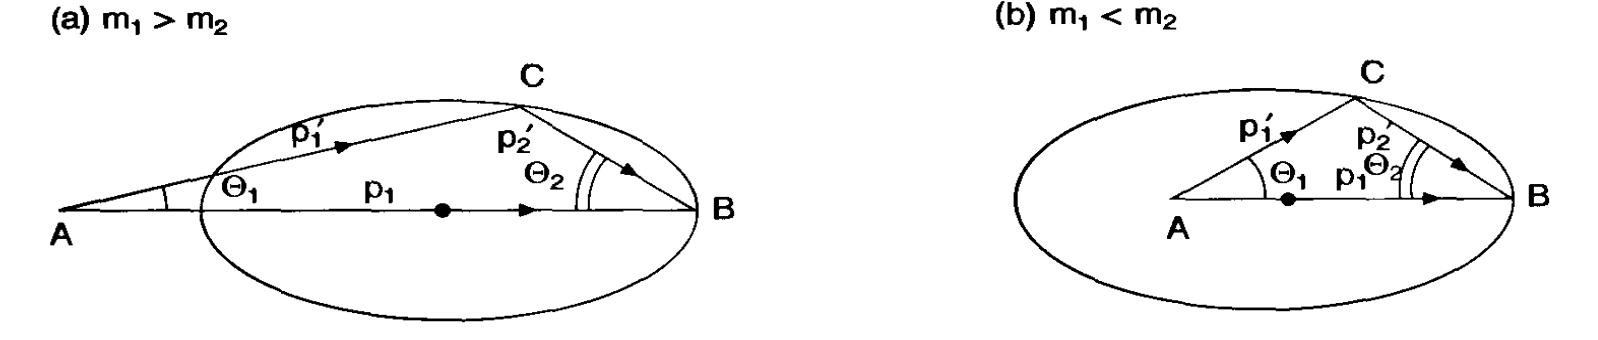
\includegraphics[height=3.4cm ,width=15.98cm]{CFT/scattering.png}
	\caption{Relativistic scattering}
\end{figure}

\chapter{Classical field theory}
\section{Lagrangian formulation}
\[S = \int \mathcal{L}(\phi_a,\dot{\phi}_a,\nabla \phi_a) d^4 x, \ \ \ \ \delta \phi_a |_{\Sigma} = 0\]
\[\delta S = 0 \Rightarrow \partial_{\mu} \left (\frac{\partial \mathcal{L}}{\partial (\partial_{\mu} \phi_a)} \right ) - \frac{\partial \mathcal{L}}{\partial \phi_a} = 0\]
\subsubsection{Locality of the theory}
There are no terms in the Lagrangian coupling $\phi(\bm{x},t)$ directly to  $\phi(\bm{y},t)$ with $\bm{x} \neq \bm{y}$. The closet we get for the $\bm{x}$ label is coupling between $\phi(\bm{x},t)$ and $\phi(\bm{x}+\delta\bm{x},t)$ through the gradient term $\bm{\nabla} \phi$.
\subsubsection{Lorentz invariance}

Scalar fields:
\[\overline{\phi}(x) = \phi(\Lambda^{-1} x)\]
Vector fields:
\[\overline{A}^{\mu}(x) = \Lambda^{\mu}_{\phantom{\mu}\nu} A^{\nu}(\Lambda^{-1}x)\]
\[\overline{A}_{\mu}(x) = (\Lambda^{-1})^{\nu}_{\phantom{\mu}\mu} A_{\nu}(\Lambda^{-1}x) = \Lambda_{\mu}^{\phantom{\mu}\nu}A_{\nu}(\Lambda^{-1}x)\]
\[\overline{\partial_{\mu}\phi}(x) = (\Lambda^{-1})^{\nu}_{\phantom{\mu}\mu} \partial_{\nu} \phi (\Lambda^{-1}x) = \Lambda_{\mu}^{\phantom{\mu}\nu} \partial_{\nu} \phi (\Lambda^{-1}x)\]
Lagrangian is a scalar, or more loosely, action is invariant under Lorentz transformation.

\section{Symmetry and conservation law}
\begin{newthem}[Noether's theorem]
	Every continuous symmetry of the Lagrangian gives rise to a conserved current $j^{\mu}(x)$ such that the equation of motion imply $\partial_{\mu} j^{\mu} = 0$.
	Suppose that the infinitesimal transformation is
	\[\phi_a \rightarrow \phi_a + \delta \phi_a\]
	\[\mathcal{L} \rightarrow  \mathcal{L} + \delta \mathcal{L} \]
	and if $\delta \mathcal{L} = \partial_{\mu} K^{\mu}$, we can get
	\[j^{\mu} = -\frac{\partial \mathcal{L}}{\partial (\partial_{\mu} \phi_a)} \delta \phi_a + K^{\mu}\]
\end{newthem}

\subsubsection{space-time translation}
$\overline{x} = x - a$ 
\[j^{\mu} = a_{\nu} T^{\mu \nu}\]
\[T^{\mu \nu} \equiv -\frac{\partial \mathcal{L}}{\partial(\partial_{\mu}\phi_a)} \partial^{\nu} \phi_a + \eta^{\mu \nu} \mathcal{L}\]
If we define $P^{\mu} \equiv \int T^{0 \mu} d^3 x$,then we have the law of momentum conservation:
\[\frac{d P^{\mu}}{dt} = 0\]

\subsubsection{Lorentz Transformation} 

$\overline{x}^{\mu} = x^{\mu} + \delta \omega^{\mu}_{\phantom{\mu}\nu} x^{\nu}$\\
The infinitesimal Lorentz transformation can be written as $I+\delta \omega^{\mu}_{\phantom{\mu}\nu}$
\[\delta \omega^{\mu}_{\phantom{\mu}\nu} = \left[ 
\begin{matrix} 
0       & \beta_1   & \beta_2   & \beta_3   \\ 
\beta_1 & 0         & -\theta_3 & \theta_2  \\
\beta_2 & \theta_3  & 0         & -\theta_1 \\
\beta_3 & -\theta_2 & \theta_1  & 0
\end{matrix} 
\right]\]
This time, we assume that
\[\overline{\phi}_a(x) = \mathcal{S}_{a}^{\phantom{a}b}\phi_b(\Lambda^{-1}x)\]
In the limit of infinitesimal Lorentz transformation, we have
\[\mathcal{S}_{a}^{\phantom{a}b} = \delta_{a}^{\phantom{a}b}+\frac{1}{2} \delta \omega_{\alpha \beta} (\Sigma^{\alpha \beta})_{a}^{\phantom{a}b} \]
\[j^{\mu} = \frac{1}{2} M^{\mu \nu \rho}  \delta \omega_{\nu \rho}\]
\[M^{\mu \nu \rho} \equiv x^{\nu}T^{\mu \rho} - x^{\rho} T^{\mu \nu} - \frac{\partial \mathcal{L}}{\partial (\partial_{\mu}\phi_a)}(\Sigma^{\nu \rho})_{a}^{\phantom{a}b}\phi_b\]
If we define $M^{\nu \rho} \equiv \int M^{0 \nu \rho} d^3 x$, then we have the law of angular momentum conservation:
\[\frac{dM^{\nu \rho}}{dt} = 0\]

\section{Functional derivatives}
\begin{newdef}[Functional derivatives]
	Given a manifold $M$ representing (continuous/smooth) functions $\rho$ (with certain boundary conditions etc.), and a functional $F$ defined as
	\[F\colon M\rightarrow \mathbb {R} \quad {\mbox{or}}\quad F\colon M\rightarrow \mathbb {C} \,,\]
	the functional derivative of $F[\rho]$, denoted $\frac{\delta F}{\delta \rho}$,is defined by
	\[{\begin{aligned}\int {\frac {\delta F}{\delta \rho }}(x)\phi (x)\;dx&=\lim _{\varepsilon \to 0}{\frac {F[\rho +\varepsilon \phi ]-F[\rho ]}{\varepsilon }}\\&=\left[{\frac {d}{d\epsilon }}F[\rho +\epsilon \phi ]\right]_{\epsilon =0},\end{aligned}}\]
	where $\phi$ is an arbitrary function. The quantity $\epsilon \phi$ is called the variation of $\rho$. 
\end{newdef}
Like the derivative of a function, the functional derivative satisfies the following properties, where $F[\rho]$ and $G[\rho]$ are functionals:\\
Linearity:
\[{\frac {\delta (\lambda F+\mu G)[\rho ]}{\delta \rho (x)}}=\lambda {\frac {\delta F[\rho ]}{\delta \rho (x)}}+\mu {\frac {\delta G[\rho ]}{\delta \rho (x)}},\]
where $\lambda$, $\mu$ are constants.\\
Product rule:
\[{\frac {\delta (FG)[\rho ]}{\delta \rho (x)}}={\frac {\delta F[\rho ]}{\delta \rho (x)}}G[\rho ]+F[\rho ]{\frac {\delta G[\rho ]}{\delta \rho (x)}}\,,\]
Chain rules:\\
If $F$ is a functional and $G$ an operator, then
\[{\displaystyle \displaystyle {\frac {\delta F[G[\rho ]]}{\delta \rho }(y)}=\int dx{\frac {\delta F[G[\rho]]}{\delta G[\rho]}}(x)\cdot {\frac {\delta G[\rho ]}{\delta \rho}(x,y)}\ }\]
If $G$ is an ordinary differentiable function $g$, then this reduces to
\[{\displaystyle \displaystyle {\frac {\delta F[g(\rho )]}{\delta \rho}(y)}={\frac {\delta F[g(\rho )]}{\delta g[\rho ]}(y)}\ {\frac {dg(\rho )}{d\rho }(y)}\ } \]
\begin{newprop}[Properties of functional derivatives]
	\[\frac{\delta F}{\delta \rho} (y) = \lim_{\epsilon \to \infty} \frac{1}{\epsilon} \{ F[\rho(x) + \epsilon \delta(x-y)] - F[\rho(x)] \}\]
	\[\frac{\delta f(x)}{\delta f(y)} = \delta(x-y)\]
	\[\frac{\delta}{\delta f(y)} \int g\left( f(x)\right) dx =  g'(f(y))\]
	\[\frac{\delta f'(x)}{\delta f(y)} = \frac{d}{dx}\delta(x-y)\]
	\[\frac{\delta}{\delta f(y)} \int g\left( f'(x)\right) dx = -\frac{d}{dy} g'(f'(y))\]
\end{newprop}

\section{Hamiltonian formulation}
\[\pi^a(x) = \frac{\partial \mathcal{L}}{\partial \dot{\phi_a}}\]
\[\mathcal{H}(\phi_a,\nabla \phi_a,\pi^a) = \pi^a \dot{\phi_a} - \mathcal{L}\]
\[H = \int \mathcal{H} d^3 x\]
Now, we can get the Hamilton equation form $\delta S =0$,
\[\dot{\phi_a}(\bm{x},t) = \frac{\delta}{\delta \pi^a(\bm{x},t)} H = \frac{\partial \mathcal{H}}{\partial \pi^a}\]
\[\dot{\pi^a}(\bm{x},t) = -\frac{\delta}{\delta \phi_a(\bm{x},t)} H = - \frac{\partial \mathcal{H}}{\partial \phi_a} + \left(\frac{\partial \mathcal{H}}{\partial \phi_{a,b}}\right)_{,b}\]

\subsection{Poission bracket}

First, we define that
\[[\phi_a(\bm{x}),\phi_b(\bm{y})] \equiv [\pi^a(\bm{x}),\pi^b(\bm{y})] \equiv 0\]
\[[\phi_a(\bm{x}),\pi^b(\bm{y})] \equiv \delta^{b}_{a} \delta(\bm{x}-\bm{y})\]
then, we demand that the bracket operation has the same properties as the Poission bracket in classical mechanics. And we also demand that
\[[\partial_x A(\bm{x}),B(\bm{y})] = \partial_x [A(\bm{x}),B(\bm{y})]\]
and
\[\left[\int d^3 x A(\bm{x}),B(\bm{y})\right] = \int d^3 x [A(\bm{x}),B(\bm{y})]\]
As a result, we can verify that
\[[W[\phi(\bm{x}),\pi(\bm{x})],Z[\phi(\bm{x}),\pi(\bm{x})]] = \int d^3x \left\{ \frac{\delta W}{\delta \phi(\bm{x})} \frac{\delta Z}{\delta \pi(\bm{x})} - \frac{\delta W}{\delta \pi(\bm{x})} \frac{\delta Z}{\delta \phi(\bm{x})} \right\}\]
Especially,
\[[\phi_a(\bm{x}),H] = \frac{\delta }{\delta \pi^a(\bm{x})} H, \ \ \ \ [\pi^a(\bm{x}),H] = -\frac{\delta }{\delta \phi_a(\bm{x})} H\]
So, the Hamilton equation can be written as
\[\dot{\phi_a} = [\phi_a,H], \ \ \ \ \dot{\pi^a} = [\pi^a,H]\]
Further more, we can prove that
\[\frac{dO(\phi,\pi,t)}{dt} = [O,H] + \frac{\partial O}{\partial t}\]
and
\[\frac{d[A,B]}{dt} = [A,\frac{dB}{dt}] + [\frac{dA}{dt},B]  \]

\subsection{Momentum}

It is easy to verify that
\[P^{0} = H, \ \ \ \ P^{i} = \int -\pi^a \partial^i \phi_a d^3 x\]
And we can get the Poisson bracket
\begin{eqnarray}
	\left[\phi_a,P^{\mu}\right] &=& -\partial^{\mu} \phi_a \nonumber \\
	\left[\pi^a,P^{\mu}\right] &=& -\partial^{\mu} \pi^a \nonumber \\
	\left[P^{\mu},P^{\nu}\right] &=& 0 \nonumber 
\end{eqnarray}


\subsection{Angular momentum}

It is easy to verify that
\[M^{\mu \nu} = \int (x^{\mu}T^{0\nu}-x^{\nu}T^{0\mu}-\pi^a(\Sigma^{\mu \nu})_{a}^{\phantom{a}b}\phi_b) d^3 x\]
We define that
\[M_{L}^{\mu \nu} \equiv \int (x^{\mu}T^{0\nu}-x^{\nu}T^{0\mu}) d^3 x \quad M_S^{\mu \nu} \equiv \int (-\pi^a(\Sigma^{\mu \nu})_{a}^{\phantom{a}b}\phi_b) d^3 x\]
\[(L^{\mu \nu})_a^{\phantom{a}b} \equiv -(x^{\mu}\partial^{\nu}-x^{\nu}\partial^{\mu})\delta_a^{\phantom{a}b} \quad (S^{\mu \nu})_a^{\phantom{a}b} \equiv -(\Sigma^{\mu \nu})_a^{\phantom{a}b}\]
So, we can get the Poisson bracket
\[[\phi_a,M_L^{\mu \nu}] = (L^{\mu \nu})_a^{\phantom{a}b} \phi_b \quad [\phi_a,M_S^{\mu \nu}] = (S^{\mu \nu})_a^{\phantom{a}b} \phi_b\]
\[[\pi^a,M_L^{\mu \nu}] = (L^{\mu \nu})_b^{\phantom{b}a}\pi^{b}  \quad [\pi^a,M_S^{\mu \nu}] = - (S^{\mu \nu})_b^{\phantom{b}a} \pi^b \]
Because $\frac{d M^{\mu \nu}}{dt} = 0$, $M^{\mu \nu}$ can commutate with $\frac{d}{dt}$, so
\[[[\phi(x),M^{\mu \nu}],M^{\rho \sigma}] = (L^{\mu \nu}+S^{\mu \nu})(L^{\rho \sigma}+S^{\rho \sigma})\phi(x)\]
At last, we can get the Poisson bracket 
\[[\phi(x),[M^{\mu \nu},M^{\rho \sigma}]] = (L^{\mu \nu}L^{\rho \sigma}-L^{\rho \sigma}L^{\mu \nu} + S^{\mu \nu}S^{\rho \sigma}-S^{\rho \sigma}S^{\mu \nu})\phi(x)\]
Since we can prove that
\[L^{\mu \nu}L^{\rho \sigma}-L^{\rho \sigma}L^{\mu \nu} = -\eta^{\nu \rho}L^{\mu \sigma} + \eta^{\sigma \mu}L^{\rho \nu} + \eta^{\mu \rho}L^{\nu \sigma} - \eta^{\sigma \nu}L^{\rho \mu}\]
if we demand that
\[S^{\mu \nu}S^{\rho \sigma}-S^{\rho \sigma}S^{\mu \nu} = -\eta^{\nu \rho}S^{\mu \sigma} + \eta^{\sigma \mu}S^{\rho \nu} + \eta^{\mu \rho}S^{\nu \sigma} - \eta^{\sigma \nu}S^{\rho \mu}\]
We will get get the Poisson bracket of the $M^{\mu \nu}$,
\[[M^{\mu \nu},M^{\rho \sigma}] = -\eta^{\nu \rho}M^{\mu \sigma} + \eta^{\sigma \mu}M^{\rho \nu} + \eta^{\mu \rho}M^{\nu \sigma} - \eta^{\sigma \nu}M^{\rho \mu}\]
up to the possibility of a term on the right-hand side that commutes with $\phi(x)$ and its derivatives.\\ \\
We now define $J_i \equiv \frac{1}{2} \epsilon_{ijk} M^{jk}$ and $K_i \equiv M^{i0}$, so we have
\[M^{\mu \nu} = \left[ 
\begin{matrix} 
0   & -K_1 & -K_2 & -K_3 \\ 
K_1 & 0    & J_3  & -J_2 \\
K_2 & -J_3 & 0    &  J_1 \\
K_3 & J_2  & -J_1 &  0
\end{matrix} 
\right] \quad \left( 
\delta \omega_{\mu\nu} = \left[
\begin{matrix} 
0       & -\beta_1   & -\beta_2   & -\beta_3   \\ 
\beta_1 & 0         & -\theta_3 & \theta_2  \\
\beta_2 & \theta_3  & 0         & -\theta_1 \\
\beta_3 & -\theta_2 & \theta_1  & 0
\end{matrix} 
\right] \right)\] 
the Poisson bracket can be written as
\begin{eqnarray}
	\left[J_i,J_j\right] &=& \epsilon_{ijk}J_k \nonumber \\
	\left[J_i,K_j\right] &=& \epsilon_{ijk}K_k \nonumber \\
	\left[K_i,K_j\right] &=& -\epsilon_{ijk}J_k \nonumber
\end{eqnarray}
We can use the similar method to derive that
\[[P^{\mu},M^{\rho \sigma}] = \eta^{\mu \sigma}P^{\mu} - \eta^{\mu \rho}P^{\sigma}\]
It can also be written as
\begin{eqnarray}
	\left[J_i,H\right] &=& 0 \nonumber \\
	\left[J_i,P_j\right] &=& \epsilon_{ijk}P_k \nonumber \\
	\left[K_i,H\right] &=& P_i \nonumber \\
	\left[K_i,P_j\right] &=& \delta_{ij}H \nonumber
\end{eqnarray}
At last, we define $L_i \equiv \frac{1}{2} \epsilon_{ijk} M_L^{jk}$ and $S_i \equiv \frac{1}{2} \epsilon_{ijk} M_S^{jk}$
we can demonstrate that
\begin{eqnarray}
	\left[L_i,S_j\right] &=& 0 \nonumber \\
	\left[S_i,P_j\right] &=& 0 \nonumber \\
	\left[L_i,P_j\right] &=& \epsilon_{ijk}P_k \nonumber
\end{eqnarray}

\chapter{Classical Electrodynamics}
\section{The formulation of classical electrodynamics}
\subsection{Maxwell equations and Lorentz force}

The Lagrangian of the EM field $A^{\mu}$ when coupling with current is
\[\mathcal{L} = -\frac{1}{4}F^{\mu\nu}F_{\mu\nu} + j^{\mu} A_{\mu}\]
Here
\[F_{\mu\nu} = \partial_{\mu}A_{\nu} - \partial_{\nu}A_{\mu} \quad j^{\mu} = \rho_{e0} u^{\mu}\]
$\rho_{e0}$ is the charge density measured in the frame of charge.
Then we can derive the Euler-Lagrange equation of EM field:
\[\partial_{\nu} F^{\mu\nu} = j^{\mu}\]
And we can derive the charge conservation equation
\[\partial_{\mu} j^{\mu} = 0\]
For a charged particle moving in EM field with orbit $x^{\mu}(\tau)$, we have
\[j^{\mu} =  e_a \delta(\bm{r}-\bm{r}_a(t)) \sqrt{1-\bm{v}_a^2} u_a^\mu \]
Then we can derive that
\[\int dV dt j^{\mu} A_{\mu} = \int dx^{\mu} e A_{\mu}\]
So, the action for a charged particle when coupling with EM field is
\[S = - m \int d\tau + e\int dx^{\mu} A_{\mu}\]
We can derive the Euler-Lagrangian equation of the particle:
\[ma_{\mu} = eF_{\mu \nu}u^{\nu}\]
The Hamiltonian formulation of electrodynamics will be discussed in detail in the Hamiltonian formulation of general relativity and canonical quantization formulation of quantum electrodynamics.\\
We now define the electric field and magnetic field as follows,
\[E^i \equiv F^{0i} = -\dot{A}^i - \nabla^i A^0 \quad B^i \equiv \epsilon_{ijk} \nabla^j A^k\]
We also define $\rho_e \equiv j^0$ and $J^i \equiv j^i$,so
the field equation can then be written
\begin{eqnarray}
	\bm{\nabla} \times  \bm{B} &=& \frac{\partial \bm{E}}{\partial t} +  \bm{J} \nonumber \\
	\bm{\nabla} \times \bm{E} &=& -\frac{\partial \bm{B}}{\partial t} \nonumber \\
	\bm{\nabla} \cdot \bm{E} &=& \rho_e \nonumber \\
	\bm{\nabla} \cdot \bm{B} &=& 0 \nonumber
\end{eqnarray}
That is the so-called Maxwell equation.\\
The equation of motion of the charged particle can be written as
\[\frac{d\bm{p}}{dt} = e(\bm{E} + \bm{v} \times \bm{B}) \quad \frac{d \mathcal{E}}{dt} = e \bm{E} \cdot \bm{v}\]
That is the so-called Lorentz force.\\
We note that the Field $A$ cannot be completely determined by Maxwell and Lorentz equation. If we make the transformation $A_{\mu} \to A_{\mu} + \partial_{\mu} \xi(x)$, $\mathcal{L}$ and $F^{\mu\nu}$ would be invariant, and the Maxwell and Lorentz equation is still valid. This arbitrariness of $\xi$ is called gauge invariance. The topic will be discussed in detail in QED.

\subsection{Lorentz transformation of fields}

In the new coordinate system $\overline{x}^{\mu} = \Lambda^{\mu}_{\phantom{\mu}\nu}x^{\nu}$, we have
\[\overline{A}^{\mu}(\overline{x}) = \Lambda^{\mu}_{\phantom{\mu}\nu}A^{\nu}(\Lambda^{-1}\overline{x})\]
In a special case when the new reference frame move along $\hat{1}$ direction with velocity $\beta$, we have
\[\overline{x}^{0} = \gamma x^0 - \gamma \beta x^1 \quad \overline{x}^{1} = -\gamma \beta x^0 + \gamma x^1\]
So, we have
\[\overline{A}^{0} = \gamma A^0 - \gamma \beta A^1 \quad \overline{A}^{1} = -\gamma \beta A^0 + \gamma A^1\]
We can further derive that
\[\overline{E}_1 = E_1 \quad \overline{E}_2 = \gamma E_2 - \gamma \beta B_3 \quad \overline{E}_3 = \gamma E_3 + \gamma \beta B_2\]
\[\overline{B}_1 = B_1 \quad \overline{B}_2 = \gamma B_2 + \gamma \beta E_3 \quad \overline{B}_3 = \gamma B_3 - \gamma \beta E_2\]
It can be written in the three vector form as
\[\bm{\overline{E}} = \gamma(\bm{E}_{\perp} + \bm{\beta} \times \bm{B}) + \bm{E}_{\parallel}\]
\[\bm{\overline{B}} = \gamma(\bm{B}_{\perp} - \bm{\beta} \times \bm{E}) + \bm{B}_{\parallel}\]
If $\beta \ll 1$, neglect the higher order of $\beta^2$, we have
\[\bm{\overline{E}} = \bm{E} + \bm{\beta} \times \bm{B}\]
\[\bm{\overline{B}} = \bm{B} - \bm{\beta} \times \bm{E}\]
We also note that $F_{\mu\nu}F^{\mu\nu}$ and $\epsilon_{\mu\nu\rho\sigma}F^{\mu\nu}F^{\rho\sigma}$ is invariant under Lorentz transformation. It can be represented by the electric and magnetic field as
\[E^2 - B^2 = \mbox{ inv } \quad \bm{E} \cdot \bm{B} = \mbox{ inv }\]

\subsection{Energy-momentum tensor}

For a free EM field, the energy-momentum tensor is
\[T_f^{\mu \nu} \equiv -\frac{\partial \mathcal{L}}{\partial(\partial_{\mu}A_{\rho})} \partial^{\nu} A_{\rho} + \eta^{\mu \nu} \mathcal{L} = \partial^{\nu}A^{\rho} F^{\mu}_{\phantom{\rho}\rho}-\frac{1}{4}\eta^{\mu\nu}F_{\rho\sigma}F^{\rho\sigma}\]
We note that the energy-momentum tensor defined above is not symmetric, so we define a modified energy-momentum tensor by adding a term $-\partial^{\rho}A^{\nu}F^{\mu}_{\phantom{\rho}\rho}$,so
\[T_e'^{\mu\nu} = F^{\nu\rho}F^{\mu}_{\phantom{\rho}\rho}-\frac{1}{4}\eta^{\mu\nu}F_{\rho\sigma}F^{\rho\sigma}\]
Note that for free EM field, $\partial^{\rho}A^{\nu}F^{\mu}_{\phantom{\rho}\rho} = \partial^{\rho}\left(A^{\nu}F^{\mu}_{\phantom{\rho}\rho}\right)$.So,
we can get that
\[\partial_{\mu}T_f'^{\mu\nu} = 0 \quad P_f'^{\mu} = P_f^{\mu}\]
So, from now on, we will use $T_f'$ as the energy-momentum tensor of EM field and omit the prime of $T_f'$ for simplicity.
The momentum of the free EM field is
\[P_f^{0} = \int dV \frac{1}{2}(\bm{E}^2+\bm{B}^2) \equiv \int dV w \quad P_f^{i} = \int dV \bm{E} \times \bm{B} \equiv \int dV \bm{S}\]\\
If there also exists charged particles in the system, i.e. the source of EM field, we must also include the energy-momentum tensor of the particles to get the right conservation equation. The energy-momentum tensor of particles is defined as
\[T_p^{\mu\nu} \equiv \sum_a m_a \delta(\bm{r}-\bm{r}_a) \sqrt{1-\bm{v}_a^2} u_a^\mu u_a^{\nu}\]
In this definition, we have
\[P_p^0 = \sum_a \frac{m_a}{\sqrt{1-\bm{v}_a^2}} \quad \bm{P}_p =  \sum_a \frac{m_a}{\sqrt{1-\bm{v}_a^2}} \bm{v}_a\]
So, our definition is consistent with the definition of four momentum in previous chapter.
Recall that
\[j^{\mu}_e = \sum_a e_a \delta(\bm{r}-\bm{r}_a) \sqrt{1-\bm{v}_a^2} u_a^\mu \]
We can define the mass current as
\[j^{\mu}_m \equiv \sum_a m_a \delta(\bm{r}-\bm{r}_a) \sqrt{1-\bm{v}_a^2} u_a^\mu \]
If there is no particle creation and annihilation, and the mass of the particle is constant during the motion, we would have
\[\partial_{\mu} j^{\mu}_{ma} = 0\]
Recall the Lorentz force equation $m a_{\mu} = eF_{\mu\nu}u^{\nu}$, it can be rewritten as
\[\rho_{m0a} \frac{du_{\mu}}{d\tau} = F_{\mu\nu}j_{ea}^{\nu}\]
Here, $\rho_{m0a} \equiv m_a \delta(\bm{r}-\bm{r}_a) \sqrt{1-\bm{v}_a^2}$ is the mass density measured in the rest frame of the particle. Then, on the one hand, we have
\[\partial_{\mu} T_p^{\mu\nu} = \sum_a \rho_{m0a}u^{\mu} \frac{\partial u_a^{\nu}}{\partial x^{\mu}} = \sum_a \rho_{m0a} \frac{d u_a^{\nu}}{d \tau} = F^{\nu}_{\phantom{\nu}\mu}j_e^{\mu}\]
On the other hand, we can derive that
\[\partial_{\mu} T_f^{\mu\nu} = - F^{\nu}_{\phantom{\nu}\mu}j_e^{\mu}\]
by implementing Maxwell equation.
Define
\[T^{\mu \nu} \equiv T_f^{\mu\nu} + T_p^{\mu\nu}\]
We have
\[\partial_{\mu} T^{\mu\nu} = 0\]
We define the Maxwell stress tensor as
\[f^{ij} \equiv -T_f^{ij} = E^{i}E^{j} + B^{i}B^{j} - w\delta^{ij}\]
Then, we can write down the conservation law of energy and momentum as
\[\frac{d}{dt}\left(P_p^0 + \int w dV \right) = -\oint \bm{S}\cdot d\bm{\sigma}\]
\[\frac{d}{dt}\left(\bm{P}_p + \int \bm{S} dV \right) = \oint \bm{f}\cdot d\bm{\sigma}\]
We assume there is no particle cross the boundary.\\
At last, because $T^{\mu\nu} = T^{\nu\mu}$, we have
\[\partial_{\mu}(x^{\nu}T^{\mu\rho}-x^{\rho}T^{\mu\nu}) = 0\]
It is easy to write down the conservation law of angular momentum as
\[\frac{d}{dt}\left(\bm{L}_p + \int \bm{r} \times \bm{S} dV \right) = \oint \bm{r} \times \bm{f}\cdot d\bm{\sigma}\]
Here,
\[\bm{L}_p = \sum_a \frac{m_a}{\sqrt{1-\bm{v}_a^2}} \bm{r}_a  \times \bm{v}_a \]

\subsection{Charged particles in a given EM field}
Now we suppose the EM field is given, i.e. we will neglect the EM field generated by the test charged particles. Then we have
\[S = \int_{t_1}^{t_2} (-\sqrt{1-v^2}m + e\bm{A}\cdot\bm{v}-e\phi)dt\]
So,
\[L = -\sqrt{1-v^2}m + e\bm{A}\cdot\bm{v}-e\phi\]
The canonical momentum is
\[\bm{\pi} = \frac{\partial L}{\partial \bm{v}} = \gamma m \bm{v} + e \bm{A}\]
The Hamiltonian is therefore
\[H = \bm{\pi} \cdot \bm{v} - L = \gamma m + e \phi = \sqrt{m^2+(\bm{\pi}-e\bm{A})^2}+e\phi\]
If $v \ll 1$, we would have
\[L = \frac{mv^2}{2} + e\bm{A}\cdot\bm{v}-e\phi \quad \bm{\pi} =  m \bm{v} + e \bm{A} \quad H = \frac{(\bm{\pi}-e\bm{A})^2}{2m}+e\phi\]
If the EM field is constant in time, we have
\[\bm{\nabla} \times \bm{E} = 0\]
we would choose the gauge that
\[\dot{\bm{A}} = 0 \quad \bm{E} = -\bm{\nabla} \phi\]
Because $\frac{\partial L}{\partial t}=0$, we can know that $\gamma m + e\phi$ is a constant.\\
Now we would list some special case.
\subsubsection{Motion in a uniform and constant electric field}
Suppose the the direction of electric field is  $\hat{x}$, the orbit is in the $x-y$ plane. So, the equation of motion is
\[\dot{p}_x = eE \quad \dot{p}_y = 0\]
The final solution is
\[x = \frac{1}{eE}\sqrt{\mathcal{E}_0^2 + (eEt)^2} \quad y = \frac{p_0}{eE} \mathrm{arcsinh} \frac{eEt}{\mathcal{E}_0}\]
Here, we assume when $t=0$, $p_x = 0$,$p_y=p_0$.
The orbit function is
\[x = \frac{\mathcal{E}_0}{eE}\cosh \frac{eEy}{p_0}\]
\subsubsection{Motion in a uniform and constant magnetic field}
Suppose the direction of magnetic field is $\hat{z}$. Note that particle's kinetic energy $\mathcal{E} = \gamma m$ is constant if there are no electric field, we can derive the equation of motion
\[\dot{v}_x = \omega v_y \quad \dot{v}_y = -\omega v_x \quad \dot{v}_z = 0\]
Here, $\omega = \frac{eB}{\gamma m}$. The final solution is
\[x = x_0 + r\sin(\omega t + \alpha) \quad y = y_0 + r\cos(\omega t + \alpha) \quad z = z_0 + v_{0z}t\]
Here, $x_0,y_0,z_0,r,\alpha,v_{0z}$ should be determined by initial condition.
\subsubsection{Motion in a uniform and constant EM field}
We only focus on the case that the velocity of particle is much smaller the velocity of light. Suppose the direction of magnetic field is $\hat{z}$, the direction of electric field is within $y-z$ plane. The equation of motion is
\[m\ddot{x} = eB\dot{y} \quad m\ddot{y} =eE_y - eB\dot{x} \quad m\ddot{z}=eE_z\]
The solution is
\[\dot{x} = a \cos \omega t + \frac{E_y}{B} \quad \dot{y} = -a\sin \omega t \quad \dot{z} = v_{0z} + \frac{eE}{m}t\]
Here, $\omega = \frac{eB}{m}$ , $a,v_{z0}$ is determined by initial condition. As we suppose that $v \ll 1$ is satisfied,we must have that
\[a \ll 1 \quad v_{0z} \ll 1 \quad \frac{eE_z t}{m} \ll 1 \quad E_y \ll B\]

\section{Constant electromagnetic field}
\subsection{Coulomb' law}
For constant electric field, the Maxwell equation take the form 
\[\bm{\nabla} \cdot \bm{E} = \rho_e \quad \bm{\nabla} \times \bm{E} = 0\]
So, we have
\[\bm{E} = -\bm{\nabla} \phi \quad \nabla^2 \phi = -\rho_e \]
The solution is
\[\phi(\bm{r}) = \int  \frac{\rho_e(\bm{r}')}{4\pi|\bm{r}-\bm{r}'|} dV'\]
If $\rho_e(\bm{r}') = Q \delta(\bm{r}')$, we have
\[\phi(\bm{r}) =  \frac{Q}{4\pi|\bm{r}|} \quad E(\bm{r}) = \frac{Q\bm{r}}{4\pi|\bm{r}|^3}\]
For a system of static charged particles, the total energy is
\[U = \frac{1}{2}\int E^2 dV = \frac{1}{2} \int \rho \phi dV = \frac{1}{2} \sum e_a \phi_a + \frac{1}{2}\sum e_a \Phi_a\]
Here, $\phi_a$ is the electric potential at the point where $e_a$ is located, produced by $e_a$ itself, while  $\Phi_a$ is the potential produced by other charges. It is obvious that $U_{self} = \frac{1}{2} e_a \phi_a$ is infinite, indicating that classical electrodynamics is no more valid in small distance. This problem will be solved in quantum electrodynamics: the mass of charged particle we measured is already renormalized to include the electromagnetic self energy. So, actually, we have
\[U = \frac{1}{2}\int E^2 dV - U_{self} = \frac{1}{2}\sum_{a \ne b} \frac{e_a e_b}{4\pi R_{ab}}\]
If the charged particle is moving with a constant velocity, we can derive the electric field it produced by Lorentz transformation, the final result is that
\[\bm{E} = \frac{e\bm{R}}{4\pi R^3} \frac{1-V^2}{(1-V^2\sin^2\theta)^{3/2}} \quad \bm{B} = \bm{V} \times \bm{E}\]
Here, $\bm{R}$ is the vector point from the particle to the point we measure the electric field, and $\theta$ is the angle between $\bm{V}$ and $\bm{R}$.If $V \sim 1$, the electric field will be concentrated in the direction perpendicular to the $\bm{V}$. If $\bm{V} \ll 1$, we have
\[\bm{E} = \frac{e\bm{R}}{4\pi R^3} \quad \bm{B} = \frac{e\bm{V} \times\bm{R}}{4\pi R^3}\]

\subsection{Multipole moments}
For a system of charged particles, the potential it produced at $\bm{R}$ is
\[\phi = \sum_a \frac{e_a}{4\pi|\bm{R} - \bm{r}_a|}\]
If $R \gg r_a$, we can expand the equation around $r_a=0$. Generally, we have
\[\frac{1}{|\bm{R} - \bm{r}|} = \sum_{l=0}^{\infty} \sum_{m=-l}^{l} \frac{r^l}{R^{l+1}} \frac{4\pi}{2l+1} Y^*_{lm}(\Theta,\Phi)Y_{lm}(\theta,\phi)\]
So,we have
\[\phi = \sum \phi^{(l)}\]
Here,
\[\phi^{(l)} = \frac{1}{4\pi R^{l+1}} \sum_{m=-l}^{l} \sqrt{\frac{4\pi}{2l+1}} Q_{m}^{(l)} Y^*_{lm}(\Theta,\Phi)\]
\[Q_m^{(l)} =\sum_a e_a r_a^l \sqrt{\frac{4\pi}{2l+1}} Y_{lm}(\theta_a,\phi_a)\]
Special case: 
\[\phi^{(0)} = \frac{Q}{4\pi R} \quad E^{(0)} = \frac{Q\bm{n}}{4\pi R^2} \quad Q = \sum_a e_a\]
\[\phi^{(1)} = \frac{\bm{d} \cdot \bm{n}}{4\pi R^2}  \quad E^{(1)} = \frac{3(\bm{d}\cdot\bm{n})\bm{n}-\bm{d}}{4\pi R^3} \quad \bm{d} = \sum_a e_a \bm{r}_a\]
\[\phi^{(2)} = \frac{\bm{n} \cdot \bm{D} \cdot \bm{n}}{8\pi R^3} \quad E^{(2)} = \frac{5(\bm{n} \cdot \bm{D} \cdot \bm{n})\bm{n} - (\bm{n} \cdot \bm{D} + \bm{D} \cdot \bm{n})}{8\pi R^4} \quad D_{ij} = \sum e(3x_ix_j-r^2\delta_{ij})\]
For a system of charged particles in the electric field $\phi(\bm{r})$, if all the particles is near the $r=0$, we can make the expansion
\[\phi(\bm{r}) = \sum_{l=0}^{\infty} r^l \sum_{m=-l}^{m=l} a_{lm} \sqrt{\frac{4\pi}{2l+1}} Y_{lm}(\theta,\phi)\]
So
\[U = \sum_{l=0}^{\infty} U^{(l)} \quad U^{(l)} = \sum_{m=-l}^{l} a_{lm}Q^{(l)}_m\]
Special case:
\[U^{(0)} = Q\phi_0 \quad F^{(0)} = Q\bm{E}_0\]
\[U^{(1)} = -\bm{d}\cdot \bm{E}_0 \quad F^{(1)} = \bm{d}\cdot \bm{\nabla}\bm{E}_0 \quad M^{(1)} = \bm{d} \times \bm{E}_0\]
\[U^{(2)} = -\frac{1}{6}\bm{D}\cdot \bm{\nabla}\bm{E}_0 \quad F^{(2)} = \frac{1}{6} \bm{D}\cdot \bm{\nabla}\bm{\nabla}\bm{E}_0 \quad M^{(2)} = \frac{1}{3} \bm{\nabla} \cdot (\bm{D} \times \bm{E}_0)\]

\subsection{Biot-Savart law}
Let us consider the magnetic field produced by charges which perform a finite motion, in which the particles are always within a finite region of space and the momenta also always remain finite. Consider the time average magnetic field $\overline{\bm{B}}$ , produced by the charges; this field will now be a function only of the coordinates and not of the time. We take the time average of the Maxwell equations
\[\bm{\nabla} \cdot \bm{B} = 0 \quad \bm{\nabla} \times \bm{B} = \frac{\partial \bm{E}}{\partial t} + \bm{j}\] 
Note that the average value of the derivative $\partial \bm{E} / \partial t$, like the derivative of any quantity which varies over a finite range, is zero. We can get
\[\bm{\nabla} \cdot \overline{\bm{B}} = 0 \quad \bm{\nabla} \times \overline{\bm{B}} =  \overline{\bm{j}}\]
Recall that $\bm{B} = \bm{\nabla} \times \bm{A}$. We impose the gauge condition $\bm{\nabla} \cdot \bm{A} = 0$, we have
\[\nabla^2 \overline{\bm{A}} = - \overline{\bm{j}}\]
The solution is
\[\overline{\bm{A}}(\bm{r}) = \frac{1}{4\pi} \int \frac{\overline{\bm{j}}(\bm{r}')}{|\bm{r}-\bm{r}'|} dV' = \frac{1}{4\pi} \sum \overline{\frac{e_a \bm{v}_a}{|\bm{r}-\bm{r}_a|}}\]
And the magnetic field is
\[\overline{\bm{B}}(\bm{r}) = \frac{1}{4\pi} \int \frac{\overline{\bm{j}}(\bm{r}') \times \bm{R}}{R^3} dV' \quad \bm{R} = \bm{r}-\bm{r}'\]

\subsection{Magnetic moment}
For a system of charged particles, the potential it produced at $\bm{R}$ is
\[\overline{\bm{A}} = \frac{1}{4\pi} \sum \overline{\frac{e_a \bm{v}_a}{|\bm{R}-\bm{r}_a|}}\]
If $R \gg r_a$, we can expand the equation around $r_a=0$ the first order,
\[4\pi \overline{\bm{A}} = \frac{1}{R} \sum e \overline{\bm{v}} - \sum \overline{e \bm{v} \left( \bm{r} \cdot \bm{\nabla} \frac{1}{R}\right)}\]
Firstly,
\[\sum e \overline{\bm{v}} = \overline{\frac{d}{dt} \sum e \bm{r}} = 0\]
Secondly,
\[-\sum \overline{e \bm{v} \left( \bm{r} \cdot \bm{\nabla} \frac{1}{R}\right)} = \frac{1}{R^3} \sum \overline{e\bm{v} (\bm{r} \cdot \bm{R})}\]
Note that
\[\sum e\bm{v} (\bm{r} \cdot \bm{R}) = \frac{1}{2} \frac{d}{dt} e\bm{r}(\bm{r}\cdot\bm{R}) + \frac{1}{2} \left(\sum e \bm{r} \times \bm{v}\right) \times \bm{R}\]
Define the magnetic moment as
\[\bm{m} \equiv \frac{1}{2} \left(\sum e \bm{r} \times \bm{v}\right)\]
We can get
\[\overline{\bm{A}} = \frac{\overline{\bm{m}} \times \bm{R}}{4\pi R^3} \quad \overline{\bm{B}} = \frac{3\bm{n}(\overline{\bm{m}} \cdot \bm{n})-\overline{\bm{m}}}{4\pi R^3}\]
If all the particles have the same charge-mass ratio, and the velocity of all the particles is much smaller than that of light, we have
\[\bm{m} = \frac{e}{2m} \sum m \bm{r} \times \bm{v} = \frac{e}{2m} \bm{M}\]
Let us consider a system of charges in an external constant uniform magnetic field. The time average of the force acting on the system, 
\[\bm{F} = \sum e \overline{\bm{v} \times \bm{B}} = \overline{\frac{d}{dt} \sum e \bm{r} \times \bm{B}} = 0\]
The average value of the moment of the forces is 
\[\overline{\bm{K}} = \sum e \overline{\bm{r} \times (\bm{v} \times \bm{B})}\]
We can derive that
\[\overline{\bm{K}} = \overline{\bm{m}} \times \bm{B}\]
Let us consider the change in the average angular momentum $\overline{\bm{M}}$ of the system. According to a well-known equation of mechanics, the derivative of $\bm{M}$ is equal to the moment $\bm{K}$ of the forces acting on the system. We therefore have
\[\frac{d \overline{\bm{M}}}{dt} = \overline{\bm{m}} \times \bm{B}\]
If the charge-mass ratio is the same for all particles of the system, the angular momentum and magnetic moment are proportional to one another, and we find:
\[\frac{d \overline{\bm{M}}}{dt} = - \bm{\Omega} \times \overline{\bm{M}} \quad \bm{\Omega} = \frac{e}{2m} \bm{B}\]
This equation states that the vector $\overline{\bm{M}}$ rotates with angular velocity $-\bm{\Omega}$ around the direction of the field, while its absolute magnitude and the angle which it makes with this direction remain fixed. This motion is called the Larmor precession.
Let us consider the Lagrangian for a system of charges in an external constant uniform magnetic field, it contains the additional term
\[L_H = \sum e \bm{A} = \sum e (\bm{B} \times \bm{r}) \cdot \bm{v} = \sum e (\bm{r} \times \bm{v}) \cdot \bm{B} = \bm{m} \cdot \bm{B}\]

\section{Electromagnetic waves}
\subsection{Electromagnetic waves}
electromagnetic fields occurring in vacuum in the absence of  charges are called electromagnetic waves. We choose the Coulomb's Gauge, i.e.
\[ \phi = 0 \quad \bm{\nabla} \cdot \bm{A} = 0\]
So,
\[\bm{E} = -\frac{\partial A}{\partial t} \quad \bm{B} = \bm{\nabla} \times \bm{A}\]
Then,from Maxwell equation we can derive that
\[\nabla^2 \bm{A} - \frac{\partial^2 \bm{A}}{\partial t^2} = 0\]
This is the equation which determines the potentials of electromagnetic waves. It is called the d'Alembert equation, or the wave equation. We can verify that the electric and magnetic fields $\bm{E}$ and $\bm{H}$ satisfy the same wave equation.\\ \\
We consider the special case of electromagnetic waves in which the fields depends only on one coordinates,say $x$,Such waves are said to be plane. In this case the equation for the field becomes
\[\frac{\partial^2 f}{\partial t^2}  - \frac{\partial^2 f}{\partial x^2} = 0\]
The solution is
\[f(t,x) = f_1(t-x) + f_2(t+x)\]
$f_1(t-x)$ represents a plane wave moving in the positive direction along the $x$ axis. $f_2(t-x)$ represents a plane wave moving in the negative direction along the $x$ axis. The Coulomb's gauge would imply that $A_x = 0$, and we can obtain
\[\bm{E} = -\bm{A}' \quad \bm{B} = -\bm{n} \times \bm{A}' = \bm{n} \times \bm{E}\]
where the prime denotes differentiation with respect to $t-x$ and $\bm{n}$ is a unit vector along the direction of propagation of the wave. We see that the electric and magnetic fields $\bm{E}$ and $\bm{B}$ of a plane wave are directed perpendicular to the direction of propagation of the wave. For this reason, electromagnetic waves are said to be transverse.\\
The energy density and flux of the plane waves are
\[W = \bm{E}^2 \quad \bm{S} = W\bm{n}\]

\subsection{Monochromatic wave}
A very important special case of electromagnetic waves is a wave in which the field is a simply periodic function of the time. Such a wave is said to be monochromatic. All quantities
(potentials, field components) in a monochromatic wave depend on the time through a factor of the form $\cos(\omega t + a)$. The quantity $\omega$ is called the cyclic frequency of the wave (we shall simply call it the frequency). For the monochromatic wave, the wave equation becomes
\[\frac{\partial^2 f}{\partial x^2} +	 \omega^2 f = 0\]
The vector potential of such a wave is most conveniently written as the real part of a complex expression
\[\bm{A} = \mathrm{Re}\left\{ \bm{A}_0 e^{i(\bm{k}\cdot\bm{r}-\omega t)}\right\} \quad \bm{k} = \omega \bm{n}\]
The electric and magnetic field are
\[\bm{E} = ik\bm{A} \quad \bm{B} = i\bm{k}\times\bm{A}\]
And we can verify that $(\omega,\bm{k})$ transform like a four-vector.\\ \\
Generally, the electric field can be  written as
\[E_y = A\cos(\phi) \quad E_z = B\cos(\phi + \delta) \quad \phi= kx -\omega t   \quad -\pi < \delta \leq \pi\]
The end of the vector $\bm{E}$ in $y-z$ plane will form an ellipse. The magnitudes of the semiaxes of the polarized ellipse are
\[|\sqrt{A^2+B^2+2AB\sin\delta} \pm \sqrt{A^2+B^2-2AB\sin\delta}|\]
The angle $\theta$ between the major axis and $y$ axis satisfies the equation
\[\tan 2\theta = \frac{2AB\cos\delta}{A^2-B^2}\]
If $-\frac{\pi}{2} < \delta < \frac{\pi}{2}$, major axis is in the second and forth quadrant. If $\delta > \frac{\pi}{2}$ or $\delta < -\frac{\pi}{2}$, major axis is in the first and third quadrant. If $\delta = \pm \frac{\pi}{2}$ and $A>B$, the major axis is $y$ axis. If $\delta = \pm \frac{\pi}{2}$ and $A<B$, the major axis is $z$ axis. If $\delta = \pm \frac{\pi}{2}$ and $A=B$, the ellipse becomes a circle.\\ 
If $0 < \delta < \pi$, the rotation is positive in the direction of $x$ axis (left handed). If $-\pi < \delta < 0$, the rotation is negative in the direction of $x$ axis(right handed). If $\delta = 0,\pi$, the ellipse becomes a line.\\ \\
Any field is expandable in a Fourier integral containing a continuous or discrete distribution of different frequencies. Such an expansion has the form
\[f(t) = \int_{-\infty}^{\infty} f_{\omega}e^{-i\omega t} \frac{d\omega}{2\pi}\]
where the Fourier components are given in terms of the function $f(t)$ by the integrals
\[f_{\omega} = \int_{-\infty}^{\infty} f(t)e^{i\omega t} dt\]
Because $f(t)$ must be real, so
\[f_{-\omega} = f_{\omega}^{*}\]
The total intensity of the wave is
\[\int_{-\infty}^{\infty} f^2 dt = \int_{-\infty}^{\infty} |f_{\omega}|^2 \frac{d\omega}{2\pi} = 2\int_{0}^{\infty} |f_{\omega}|^2 \frac{d\omega}{2\pi} \]

\subsection{Partially polarized light}
Every monochromatic wave is necessarily polarized. However we usually have to deal with waves which are only approximately monochromatic, and which contain frequencies in a small interval $\Delta \omega$. We consider such a wave, and let $\omega$ be some average frequency for it. Then its field at a fixed point in space can be written in the form
\[\bm{E_0}(t)e^{-i\omega t}\]
where the complex amplitude $\bm{E}_0$ is some slowly varying function of the time. Since $\bm{E}_0$ determines the polarization of the wave, this means that at each point of the wave, its polarization changes with time, such a wave is said to be partially polarized.\\
The polarization properties of electromagnetic waves are observed experimentally by passing the light to be investigated through various bodies and then
observing the intensity of the transmitted light. From the mathematical point of view this means that we draw conclusions concerning the polarization properties of the light from the values of certain quadratic functions of its field. Here of course we are considering the time averages of such functions.\\
Quadratic functions of the field are made up of terms proportional to the products $E_{\alpha} E_{\beta}$,
$E_{\alpha}^{*} E^{*}_{\beta}$ or $E_{\alpha}^* E_{\beta}$. Products of the form $E_{\alpha} E_{\beta}$ and
$E_{\alpha}^{*} E^{*}_{\beta}$ contain the rapidly oscillating factors $e^{-i2\omega t}$ and will give zero when the time average is taken. Thus we see that the polarization properties of the light are completely characterized by the tensor
\[J_{\alpha \beta} = E_{0\alpha} E_{0\beta}^{*}\]
The trace of the tensor
\[J \equiv J_{\alpha\alpha} = \bm{E}_0 \bm{E}^*_0\]
determines the intensity of the wave, as measured by the energy flux density.To eliminate this quantity which is not directly related to the polarization properties, we
introduce the tensor
\[\rho_{\alpha\beta} = \frac{J_{\alpha\beta}}{J}\]
we call it the polarization tensor.\\ \\
Generally, the polarization tensor is expressed as
\[\rho = \frac{1}{2} \left[ \begin{matrix} 1+p_{3}& p_1-ip_2\\ p_1+ip_2& 1-p_{3}\end{matrix} \right] \]
If we introduce the Pauli matrix, i.e.
\[\sigma_1 = \left[ \begin{matrix} 0& 1\\ 1& 0\end{matrix} \right] \quad \sigma_2 = \left[ \begin{matrix} 0& - i\\ i& 0\end{matrix} \right] \sigma_3 = \left[ \begin{matrix} 1& 0\\ 0& -1\end{matrix} \right] \]
The $\rho$ can be expressed as
\[\frac{1}{2} (1-P) I + \frac{1}{2} P(I + \bm{n} \cdot \bm{\sigma})\]
Here,
\[P = \sqrt{p_1^2 + p_2^2 + p_3^2} \quad \bm{n} = (\frac{p_1}{P},\frac{p_2}{P},\frac{p_3}{P})\]
For a totally polarized light with polarization state$ | E\rangle = (\cos \frac{\theta}{2} e^{-i\frac{\phi}{2}} , \sin \frac{\theta}{2} e^{i\frac{\phi}{2}})$, the polarization tensor $\rho = |E\rangle \langle E|$. We can verify that
\[P = 1 \quad \bm{n} = (\sin\theta \cos\phi, \sin\theta \sin\phi, \cos \theta)\]
So, for an arbitrary light,
\[\rho = (1-P)\rho_{n} + P \rho_{p} \quad \rho_n = \frac{1}{2}I \quad \rho_p = \frac{1}{2}(I + \bm{n} \cdot \bm{\sigma})\]
Thus, we call $P$ the Polarization degree. \\ \\
Suppose there is a polarizing filter,  which allow the light with polarization state
\[| D \rangle = (\cos \frac{\theta}{2} e^{-i\frac{\phi}{2}} , \sin \frac{\theta}{2} e^{i\frac{\phi}{2}})\]
to pass totally. If a light with polarization tensor $\rho$ pass through the device, the relative intensity will become
\[\langle D | \rho | D \rangle = \frac{1}{2} + \frac{1}{2} \bm{p} \cdot \bm{m}\]
Here, $\bm{p} = (p_1,p_2,p_3)$, $\bm{m} = (\sin\theta \cos\phi, \sin\theta \sin\phi, \cos \theta)$\\ \\
In optics, the Stokes vectors are defined as
The Stokes parameters are defined by
\begin{eqnarray}
I&\equiv& \langle E_{x}^{2}\rangle +\langle E_{y}^{2}\rangle \nonumber \\
&=& \langle E_{a}^{2}\rangle +\langle E_{b}^{2}\rangle \nonumber \\
&=& \langle E_{l}^{2}\rangle +\langle E_{r}^{2}\rangle \nonumber \\
Q&\equiv& \langle E_{x}^{2}\rangle -\langle E_{y}^{2}\rangle \nonumber \\
U&\equiv& \langle E_{a}^{2}\rangle -\langle E_{b}^{2}\rangle \nonumber \\
V&\equiv& \langle E_{l}^{2}\rangle -\langle E_{r}^{2}\rangle \nonumber
\end{eqnarray}
where the subscripts refer to three different bases of the space of Jones vectors: the standard Cartesian basis ${\hat {x}},{\hat {y}}$, a Cartesian basis rotated by 45° ${\hat {a}},{\hat {b}}$, and a circular basis ${\hat {l}},{\hat {r}}$. The symbols $\langle \cdot \rangle$ represent expectation values. The light can be viewed as a random variable taking values in the space $C^2$ of Jones vectors $(E_1,E_2)$. It is easy to verify that
\[Q = Ip_3 \quad U = Ip_2 \quad V = Ip_1\]
\end{document}

\part{General relativity}
\documentclass{article}
\usepackage[left=1.5cm, right=1.5cm, top=3cm, bottom = 3cm]{geometry}
\usepackage{amsmath}
\usepackage{mathrsfs}
\usepackage{amsfonts}
\usepackage{amssymb}
\usepackage{graphicx}
\usepackage{float}
\usepackage{wrapfig}
\usepackage{latexsym}
\usepackage{hyperref}
\usepackage{feynmf}
\usepackage{exscale}
\usepackage{relsize}
\usepackage{bm}%bold math, for vector
\linespread{1.1}

\usepackage{hyperref}
\hypersetup{
  pdfauthor={Yuyang Songsheng},
  pdftitle={Summary on General Relativity},
  pdfsubject={Summary on General Relativity},
  urlcolor=blue,
}




\author{Yuyang Songsheng}
\title{Summary on General Relativity}

\begin{document}
\maketitle
\section{Differential Geometry}
\subsection{Fundamental conception on differential manifolds}
\href{https://en.wikipedia.org/wiki/Manifold}{\textbf{Manifold}} 
Formally, a topological manifold is a second countable Hausdorff space that is locally homeomorphic to Euclidean space.\\
\href{https://en.wikipedia.org/wiki/Differentiable_manifold}{\textbf{Differentiable manifold}} 
In formal terms, a differentiable manifold is a topological manifold with a globally defined differential structure. \\
\href{https://en.wikipedia.org/wiki/Tangent_space}{\textbf{Tangent space}} 
In mathematics, the tangent space of a manifold facilitates the generalization of vectors from affine spaces to general manifolds, since in the latter case one cannot simply subtract two points to obtain a vector pointing from one to the other.\\
\href{https://en.wikipedia.org/wiki/Cotangent_space}{\textbf{Cotangent space}} 
Typically, the cotangent space is defined as the dual space of the tangent space at $x$.\\
\href{https://en.wikipedia.org/wiki/Submanifold}{\textbf{Submanifold}}\\
\textbf{Immersed submanifolds} An immersed submanifold of a manifold $M$ is the image $S$ of an immersion map $f:N \to M$; in general this image will not be a submanifold as a subset, and an immersion map need not even be injective (one-to-one) – it can have self-intersections.\\
\textbf{Injective immersion submanifolds} More narrowly, one can require that the map $f:N \to M$ be an inclusion (one-to-one), in which we call it an injective immersion, and define an immersed submanifold to be the image subset S together with a topology and differential structure such that S is a manifold and the inclusion f is a diffeomorphism: this is just the topology on N, which in general will not agree with the subset topology: in general the subset S is not a submanifold of M, in the subset topology.\\
\textbf{Open submanifolds}\\
\textbf{Closed submanifolds}\\
\textbf{Closed submanifolds of an open submanifold}\\
If an n dimensional injective immersed submanifold $N$ of a $m$ dimensional manifold $M$ is a closed submanifold of an open submanifold of $M$, then for every point $p \in f(N)$ there exists a chart ($U \subset M$,$\phi:U \to R_n $) containing $p$ such that $\phi(f(N) \cap U)$ is the intersection of a $n$-dimensional plane with $\phi(U)$.\\
\textbf{Embedded submanifolds} An embedded submanifold (also called a regular submanifold), is an immersed submanifold for which the inclusion map is a topological embedding. That is, the submanifold topology on $S$ is the same as the subspace topology. Given any embedding $f:N \to M$ of a manifold $N$ in $M$ the image $f(N)$ naturally has the structure of an embedded submanifold. That is, embedded submanifolds are precisely the images of embeddings. Closed submanifolds of an open submanifold are equal to embedded submanifolds.\\

\subsection{Multi linear algebra}
\textbf{Vector space}\ \ \ \ \textbf{Dual space}\\
\textbf{Tensor product}
\[V \otimes W = \mbox{ Span}\{ v \otimes w \} = \mathcal{L}(V^*,W^*;F)\]
\[V^* \otimes W^* = \mbox{ Span}\{ v^* \otimes w^* \} = \mathcal{L}(V,W;F)\]
\[\mathcal{L}(V,W;Z)=\mathcal{L}(V \otimes W;Z)\]
\[(\phi \otimes \psi)\otimes \xi = \phi \otimes (\psi \otimes \xi)\]
\textbf{Tensor}
\[V_s^r = V \otimes \cdots \otimes V \otimes V^* \otimes \cdots \otimes V^*\]
\[x=x^{i_1 \cdots i_r}_{\phantom{i_1 \cdots i_r} k_1 \cdots k_s} e_{i_1} \otimes \cdots \otimes e_{i_r} \otimes e^{*k_1} \otimes \cdots \otimes e^{*k_s}\]
\[(x \otimes y)^{i_1 \cdots i_{r_1+r_2}}_{\phantom{i_1 \cdots i_{r_1+r_2}} k_1 \cdots k_{s_1+s_2}} = 
x^{i_1 \cdots i_{r_1}}_{\phantom{i_1 \cdots i_{r_1}}k_1 \cdots k_{s_1}} \cdot y^{i_{r_1+1} \cdots i_{r_1+r_2}}_{\phantom{i_{r_1+1} \cdots i_{r_1+r_2}}k_{s_1+1} \cdots k_{s_1+s_2}}\]
\textbf{Permutation}($\sigma \in \mathcal{P}(r)$)
\[\sigma x(v^{*1},\cdots,v^{*r})=x(v^{*\sigma(1)},\cdots,v^{*\sigma(r)})\]
\textbf{Symmetric contra-variant tensor}
\[\sigma x =x\]
\textbf{Antisymmetric contra-variant tensor}
\[\sigma x =\mbox{ sgn }\sigma \cdot x\]
\textbf{Symmetrization operator}
\[S_r(x) = \frac{1}{r!} \sum_{\sigma \in \mathcal{P}(x)} \sigma x\]
\textbf{Antisymmetrization operator}
\[A_r(x) = \frac{1}{r!} \sum_{\sigma \in \mathcal{P}(x)} \mbox{ sgn }\cdot \sigma x\]
\textbf{Exterior vector space}
\[\Lambda^r(V) = A_r(T^r(V))\]
\[\Lambda^0(V)=F \ \ \ \Lambda^1(V)=V\]
\textbf{Wedge product}
\[\xi \wedge \eta \equiv \frac{(k+l)!}{k!l!}A_{k+l}(\xi \otimes \eta)\]
\[(\xi_1+\xi_2) \wedge \eta = \xi_1 \wedge \eta + \xi_2 \wedge \eta\]
\[\xi \wedge (\eta_1+\eta_2) = \xi \wedge \eta_1 + \xi \wedge \eta_2\]
\[\xi \wedge \eta = (-1)^{kl} \eta \wedge \xi\]
\[(\xi \wedge \eta) \wedge \zeta = \xi \wedge (\eta \wedge \zeta) = \frac{(k+l+h)!}{k!l!h!}A_{k+l+h}(\xi \otimes \eta \otimes \zeta)\]
\[e_{i_1} \wedge \cdots \wedge e_{i_r}(v^{*1},\cdots,v^{*r}) = \mbox{ det } \langle e_{i_{\alpha}},v^{*\beta} \rangle\]
\[e_{i_1} \wedge \cdots \wedge e_{i_r}(e^{*j_1},\cdots,e^{*j_r}) = \mbox{ det } \langle e_{i_{\alpha}},v^{*j_{\beta}} \rangle = \delta^{j_1 \cdots j_r}_{i_1 \cdots i_r}\]
\[\Lambda^r(V) = \mbox{ Span }\{e_{i_1} \wedge \cdots \wedge e_{i_r},1\leq i_1 < \cdots < i_r \leq n  \}\]
\[(\Lambda^r(V))^* = \Lambda^r(V^*)\]
\textbf{Pull-back mapping}
$f:V \to W$ is a linear mapping, we define $f^*:\Lambda^r(W^*) \to \Lambda^r(V^*)$ as
\[f^* \phi(v_1,\cdots,v_r) = \phi(f(v_1),\cdots,f(v_r)).\]
Theorem:
\[f^*(\phi \wedge \psi) = f^*\phi \wedge f^*\psi\]

\subsection{Vector Bundle}
\href{https://en.wikipedia.org/wiki/Fiber_bundle}{\textbf{Fiber bundle}} 
In mathematics, and particularly topology, a fiber bundle is a space that is locally a product space, but globally may have a different topological structure. Specifically, the similarity between a space E and a product space B × F is defined using a continuous surjective map $\pi :E \to B$ that in small regions of $E$ behaves just like a projection from corresponding regions of $B \times F$ to $B$. The map $\pi$, called the projection or submersion of the bundle, is regarded as part of the structure of the bundle. The space $E$ is known as the total space of the fiber bundle, $B$ as the base space, and $F$ the fiber.\\ \\
\href{https://en.wikipedia.org/wiki/Vector_bundle}{\textbf{Vector Bundle}} 
In mathematics, a vector bundle is a topological construction that makes precise the idea of a family of vector spaces parameterized by another space $X$ (for example $X$ could be a topological space, a manifold, or an algebraic variety): to every point $x$ of the space $X$ we associate (or "attach") a vector space $V(x)$ in such a way that these vector spaces fit together to form another space of the same kind as $X$ (e.g. a topological space, manifold, or algebraic variety), which is then called a vector bundle over $X$.\\ \\
\href{https://en.wikipedia.org/wiki/Tangent_bundle}{\textbf{Tangent bundle}} 
In differential geometry, the tangent bundle of a differentiable manifold $M$ is a manifold $TM$, which assembles all the tangent vectors in $M$. As a set, it is given by the disjoint union of the tangent spaces of $M$. That is,
\[
TM = \bigsqcup_{x \in M}T_xM = \bigcup_{x \in M} \{x\} \times T_xM = \bigcup_{x \in M}\{(x,y)| y \in T_xM \}
\]
where $T_xM$ denotes the tangent space to $M$ at the point $x$. So, an element of $TM$ can be thought of as a pair $(x,v)$ , where $x$ is a point in $M$ and $v$ is a tangent vector to $M$ at $x$. There is a natural projection $\pi : TM \to M$ defined by $\pi(x,v) = x$. This projection maps each tangent space $T_xM$ to the single point $x$.
The tangent bundle comes equipped with a natural topology. With this topology, the tangent bundle to a manifold is the prototypical example of a vector bundle (a fiber bundle whose fibers are vector spaces). A section of $TM$ is a vector field on $M$, and the dual bundle to $TM$ is the cotangent bundle, which is the disjoint union of the cotangent spaces of $M$. By definition, a manifold $M$ is parallelizable if and only if the tangent bundle is trivial. By definition, a manifold $M$ is framed if and only if the tangent bundle $TM$ is stably trivial, meaning that for some trivial bundle $E$ the Whitney sum $TM \oplus E$ is trivial. For example, the $n$-dimensional sphere $S_n$ is framed for all $n$, but parallelizable only for $n=1,3,7$ (by results of Bott-Milnor and Kervaire).\\
A smooth assignment of a tangent vector to each point of a manifold is called a vector field. Specifically, a vector field on a manifold $M$ is a smooth map $V: M \to TM$ such that the image of $x$, denoted $Vx$, lies in $T_xM$, the tangent space at $x$. In the language of fiber bundles, such a map is called a section. A vector field on $M$ is therefore a section of the tangent bundle of $M$.\\
Generalization:\\
\textbf{Cotangent bundle} $T^*M = \bigcup_{x \in M} T^*_{\phantom{*}x}M$ \\
\textbf{Tensor bundle} $T^r_sM = \bigcup_{x \in M} T^{r\phantom{x}}_{sx}M$ \\
\textbf{Exterior vector bundle} $\Lambda^rM = \bigcup_{x \in M} \Lambda^r(T_x)$\\
\textbf{Exterior form bundle} $\Lambda^rM^* = \bigcup_{x \in M} \Lambda^r(T^{*}_{\phantom{*}x})$

\subsection{Tangent vector field}
\textbf{Theorem 1} Let $M$ be a smooth manifold, and let $Y:M \to TM$ be a vector field. If $(U, (X_i))$ is any smooth coordinate chart on $M$, then $Y$ is smooth on $U$ if and only if its component functions with respect to this chart are smooth.\\
\textbf{Theorem 2} Let $M$ be a $m$ dimensional smooth manifold and $v$ a smooth tangent vector field on $M$. $v:C^{\infty}(M) \to C^{\infty}$ satisfy that\\
(1) $\forall f,g \in C^{\infty}(M),v(f+g)=v(f)+v(g)$;\\
(2) $\forall f \in C^{\infty}(M),\alpha \in \mathbf{R},v(\alpha f)=\alpha \cdot v(f)$;\\
(3) $\forall f,g \in C^{\infty}(M),v(f,g) = f \cdot v(g) + g \cdot v(f)$.\\
If $\alpha:C^{\infty}(M) \to C^{\infty}(M)$ satisfy the three conditions above, there exists a unique smooth vector field $v$ on $M$ that $\forall f \in C^{\infty}(M),v(f)=\alpha(f)$.\\ \\
\textbf{Theorem 3} $\forall X,Y \in \mathcal{H}(M),[X,Y]=X \circ Y -Y \circ X \in \mathcal{H}(M)$.\\ \\
\textbf{Useful formulas 1}\\
(1) $[aX+bY,Z]=a[X,Z]+b[Y,Z]$;$[Z,aX+bY]=a[Z,X]+b[Z,Y]$;\\
(2) $[X,Y]=-[Y,X]$;\\
(3) $[X,[Y,Z]] + [Y,[Z,Z]] +[Z,[X,Y]]=0$;\\
(4) $[X,Y]|_{U} = [X|_{U},Y|_{U}] = (X_i \frac{\partial Y^j}{\partial u^i} - Y^i \frac{\partial X^j}{\partial u^i}) \frac{\partial}{\partial u^j}$;\\
(5) $f_{*}[X,Y] = [f_{*}X,f_{*}Y]$;\\ \\
\textbf{definition 1} Let $M$ be a smooth manifold and $\phi:\mathbf{R} \times M \to M$ a smooth mapping, and $\forall (t,p) \in \mathbf{R} \times M$,denote $\phi_{t}(p) = \phi(t,p)$. If $\phi$ satisfy that\\
(1) $\phi_0 = \mathrm{id}:M \to M$;\\
(2) $\forall s,t \in \mathbf{R}, \phi_s \circ \phi_t = \phi_{s+t}$;\\
then $\phi$ is called a one parameter differentiable transformation group acting on $M$.\\
Trajectory of $\phi$ through $p$ on $M$:$\gamma_p(t) = \phi(t,p)$.\\
Vector field induced by $\phi$: $X_p(f) = \langle \gamma_p , f \rangle$.\\ \\
\textbf{Useful Formulas 2}\\
(1) $\gamma_q(t) = \phi(t,\phi(s,p)) = \phi(t+s,p) = \gamma_p(t+s)$;\\
(2) $(\phi_s)_{*}X_p = X_{\phi_s(p)}$;\\
(3) $\psi_{*} X_p = \tilde{X}_{\psi(p)}$ if $X$ is induced by $\phi$ and $\tilde{X}$ is induced by $\psi \circ \phi \circ \psi^{-1} $. $\psi$ is a smooth  homeomorphism.\\
(4) $[X,Y] = \lim_{t \to 0} \frac{Y_p-(\phi_t)_* Y_{\phi_{-t}(p)}}{t} = \lim_{t \to 0} \frac{(\phi_{-t})_*Y_{\phi_t(p)}- Y}{t}$ if $X$ is induced by $\phi$.\\ \\
\textbf{Lie derivative(1)}\\
\[\mathcal{L}_{X}Y= \lim_{t \to 0} \frac{(\phi_{-t})_*Y_{\phi_t(p)}- Y}{t} =[X,Y]\]
\[\mathcal{L}_{X}f = X(f)\]\\
\textbf{Useful Formulas 3}\\
\[\mathcal{L}_{X}(Y + \lambda Z) = \mathcal{L}_{X}Y + \lambda\mathcal{L}_{X}Z\]
\[\mathcal{L}_{X}(f \cdot Y) = \mathcal{L}_{X}(f) \cdot Y + f\mathcal{L}_{X}Y\]
\[\mathcal{L}_{X}([Y,Z]) = [\mathcal{L}_{X}Y,Z]+ [Y,\mathcal{L}_{X}Z]\]\\ \\
\textbf{Theorem 4} Let $M$ be a n-dimensional smooth manifold and $X \in \mathcal{H}(M)$. If $p \in M$ and $X_p \neq 0$, $\exists (V,x^i)$ and $p \in V$ that $X|_V = \frac{\partial}{\partial y^1 }$.\\ \\
\href{https://en.wikipedia.org/wiki/Distribution_(differential_geometry)}{\textbf{Distribution}} Let $M$ be a $C^{\infty }$  manifold of dimension $m$ , and let $n \leq m$ . Suppose that for each $x\in M$ , we assign an $n$-dimensional subspace $\Delta _{x}\subset T_{x}(M)$ of the tangent space in such a way that for a neighbourhood $N_{x}\subset M$ of $x$ there exist $n$ linearly independent smooth vector fields $X_{1},\ldots ,X_{n}$ such that for any point $y\in N_{x}$, $X_{1}(y),\ldots ,X_{n}(y)$ span $\Delta _{y}$. We let $\Delta$  refer to the collection of all the $\Delta_{x}$ for all $ x\in M$ and we then call $\Delta$ a distribution of dimension $n$ on $M$ , or sometimes a $C^{\infty }$ $n$-plane distribution on $M$. The set of smooth vector fields $\{X_{1},\ldots ,X_{n}\}$ is called a local basis of $\Delta$.\\ \\
\textbf{Involutive distributions} We say that a distribution $\Delta$ on $M$ is involutive if for every point $x \in M$ there exists a local basis $\{X_{1},\ldots ,X_{n}\}$ of the distribution in a neighbourhood of $x$ such that for all $1\leq i,j\leq n$ , $[X_{i},X_{j}]$  is in the span of $\{X_{1},\ldots ,X_{n}\}$.That is, if $[X_{i},X_{j}]$ is a linear combination of $\{X_{1},\ldots ,X_{n}\}$. Normally this is written as $ [\Delta ,\Delta ]\subset \Delta $.\\
Involutive distributions are the tangent spaces to foliations. Involutive distributions are important in that they satisfy the conditions of the Frobenius theorem, and thus lead to integrable systems.
A related idea occurs in Hamiltonian mechanics: two functions f and g on a symplectic manifold are said to be in mutual involution if their Poisson bracket vanishes.\\ \\
\textbf{Frobenius Theorem} If distribution $\Delta$ on $M$ is involutive, then $\forall p \in M$, $\exists (V,x^i)$ and $p \in V$ that $\Delta|_{V} = \mathrm{Span} \{ \frac{\partial}{\partial y^1} , \cdots, \frac{\partial}{\partial y^h}\}$.\\ \\
\textbf{Integrable manifold} Let $L^{h}$ be a smooth distribution on $M$. If $\phi:N \to M$ is an injective immersion manifold, and $\forall p \in N$, $\phi_{*}(T_pN) \subset L^h(\phi(p))$, then $(\phi,N)$ is called an integrable manifold of $L^h$.\\
If $\forall q \in M$, there is an integrable manifold of $L^h$ through it, we say that $L^h$ is completely integrable.\\ \\
\textbf{Theorem 5} Let
\[\tau: \underbrace{A^1(M) \times \cdots \times A^1(M)}_p \times \underbrace{\mathcal{H}(M) \times \cdots \times \mathcal{H}(M)}_q \to c^{\infty}(M)\] 
be a $p+q$ multi-linear mapping, if $\forall 1 \leq a \leq p,1 \leq b \leq q$ and $\mu \in C^{\infty}(M)$,
\begin{eqnarray}
&&\tau(\alpha^1,\cdots,\mu \alpha^{a},\cdots,\alpha^p,v_1,\cdots,v_q)\nonumber \\
&=&\tau(\alpha^1,\cdots,\alpha^p,v_1,\cdots,\mu v_{b},\cdots,v_q)\nonumber \\
&=&\mu \cdot \tau(\alpha^1,\cdots,\alpha^p,v_1,\cdots,v_q)\nonumber
\end{eqnarray}
then the mapping $\tau$ define a $(p,q)$ tensor for all $x \in M$ smoothly.\\ \\
\textbf{Lie derivatives(2)} Let $X$ be a smooth tangent vector field on $M$ and $\phi_t$ the one parameter differentiable transformation group inducing it. Denote the trajectory of $\phi_t$ through $x$ by $\gamma_x(t)$. So we have linear isomorphism
\[(\phi_t^{-1})_{*} = (\phi_{-t})_{*} : T_{\gamma_x(t)}M \to T_xM\]
\[(\phi_t)^* : T_{\gamma_x(t)}^* \to T_xM\]
So we can induce the linear isomorphism
\[\Phi_t: T^p_q(\gamma_x(t)) \to T^p_q(x)\]
If $S$ and $T$ are smooth tensor fields on $M$,\\
(1) for all $t$ which is small enough, $\Phi_tS$ is a smooth tensor field on $M$ which has the same type as $S$ ,and $\lim_{t \to 0} \Phi_t(S(\gamma_p(t))) = S(p),\forall p \in M$.\\
(2)$\Phi_t(S \otimes T) = \Phi_tS \otimes \Phi_tT$.\\
(3)$\Phi_t(C^a_b(S)) = C^a_b(\Phi_t(S))$, $C^a_b$ is a tag for contraction.\\
So,we can define the Lie derivative for smooth tensor field $\tau$ on $M$ as
\[\mathcal{L}_{X}(\tau) = \lim_{t \to 0}\frac{\Phi_t(\tau)-\tau}{t}\]\\
\textbf{Useful Formulas 4}
\[\mathcal{L}_X(\tau_1+\lambda \tau_2) = \mathcal{L}_X \tau_1 + \lambda \mathcal{L}_X \tau_2\]
\[\mathcal{L}_X(\tau_1 \otimes \tau_2) = \mathcal{L}_X\tau_1 \otimes \tau_2 + \tau_1 \otimes \mathcal{L}_X \tau_2\]
\[C^r_s(\mathcal{L}_X \tau) = \mathcal{L}_X(C^r_s(\tau))\]
\[(\mathcal{L}_X \omega)(Y) = X(\omega(Y)) - \omega([X,Y])\]
\[((\mathcal{L}_X \tau)|_U)^{\mu_1,\cdots,\mu_p}_{v_1,\cdots,v_q} = X^{\alpha} \partial_{\alpha} \tau^{\mu_1,\cdots,\mu_p}_{v_1,\cdots,v_q} - \sum_{i=1}^{p} \tau^{\mu_1,\cdots,\alpha,\cdots,\mu_p}_{v_1,\cdots,v_q} \partial_{\alpha} X^{\mu_i} + \sum_{j=1}^{q}\tau^{\mu_1,\cdots,\mu_p}_{v_1,\cdots,\alpha,\cdots,v_q} \partial_{v_j}X^{\alpha}\]
\[\mathcal{L}_{[X,Y]} = \mathcal{L}_X \circ \mathcal{L}_Y - \mathcal{L}_Y \circ \mathcal{L}_X \]
\[\mathcal{L}_{X+Y} = \mathcal{L}_{X} + \mathcal{L}_{Y}\]

\subsection{Exterior differential}
\textbf{Exterior form space} $A(M) = \sum_{r=0}^{m} A^{r}(M)$\\
For $\tau \in A^r(M)$,
\[\tau|_{U} = \frac{1}{r!} \tau_{i_1\cdots i_r} dx^{i_1} \wedge \cdots \wedge dx^{i_r} = \tau_{|i_1\cdots i_r|} dx^{i_1} \wedge \cdots \wedge dx^{i_r}\] 
\[ \tau_{i_1\cdots i_r} = \tau(\frac{\partial}{\partial x^{i_1}},\cdots,\frac{\partial}{\partial x^{i_r}}) \]
\begin{eqnarray}
\tau(v_1,\cdots,v_r)|_{U} &=& \tau_{|i_1\cdots i_r|}dx^{i_1} \wedge \cdots \wedge dx^{i_r} (v_1,\cdots,v_r) \nonumber \\
&=& \tau_{|i_1\cdots i_r|} \left| \begin{matrix} v_1^{i_1}& \cdots & v_r^{i_1}\\ \vdots & & \vdots \\ v_1^{i_r} & \cdots & v_r^{i_r} \end{matrix} \right| \nonumber
\end{eqnarray}
It is a $r$ multi-linear mapping, and for every variable, it is $C^{\infty}(M)$ linear.\\ \\
\textbf{Pull back mapping}\\
$f:M \to N \Rightarrow f_{*}:T_{p}M \to T_{f(p)}N \Rightarrow f^{*}:\wedge^{r}(T_{f(p)}^{*}N) \to \wedge^{r}(T_p^*M) $\\
\[f^* \phi(v_1,\cdots,v_r) = \phi(f_*v_1,\cdots,f_*v_r)\]
\[f^*\phi|_U = \frac{1}{r!}(\phi_{\alpha_1\cdots\alpha_r} \circ f) \cdot \frac{\partial f^{\alpha_1}}{\partial x^{i_1}} \cdots \frac{\partial f^{\alpha_r}}{\partial x^{i_r}} dx^{i_1} \wedge \cdots \wedge dx^{i_r}\]
\[f^*(\phi \wedge \psi) = f^*\phi \wedge f^* \psi\]\\
\textbf{Exterior differential} Let $M$ be a m-dimensional smooth manifold. Then $\exists$ a unique mapping $d:A(M) \to A(M)$ satisfy that\\
(1) $d(A^r(M)) \subset A^{r+1}(M)$\\
(2) $\forall \omega_1,\omega_2 \in A(M),d(\omega_1+\omega_2) = d\omega_1 +d\omega_2$\\
(3) if $\omega_1 \in A^r(M)$,then $d(\omega_1 \wedge \omega_2)=d\omega_1 \wedge \omega_2 +(-1)^r \omega_1 \wedge d\omega_2$\\
(4) $f \in A^0(M)$,$df$ is just the differential of $f$\\
(5) $\forall f \in A^0(M)$,$d(df)=0$\\
$d$ is called exterior differential.\\ \\
\textbf{Theorem 1}\\
$\forall \omega \in A^1(M),X,Y \in \mathcal{H}(M)$,
\[d\omega(X,Y) = X \langle Y,\omega \rangle -Y \langle X,\omega \rangle -\langle [X,Y],\omega \rangle \] 
$\forall \omega \in A^r(M)$, $X_1,\cdots,X_{r+1} \in \mathcal{H}(M)$,
\begin{eqnarray}
d\omega(X_1,\cdots,X_{r+1}) &=& \sum_{i=1}^{r+1}(-1)^{i+1} X_{i}(\langle X_1 \wedge \cdots \wedge \hat{X_i} \wedge \cdots \wedge X_{r+1},\omega \rangle) \nonumber \\
&+& \sum_{1 \leq i < j \leq r+1}(-1)^{i+j} \langle [X_i,X_j] \wedge \cdots \wedge \hat{X_i} \wedge \cdots \wedge \hat{X_j} \wedge \cdots X_{r+1},\omega \rangle
\end{eqnarray}\\
\textbf{Theorem 2} $f^{*}(d\omega) = d(f^* \omega)$\\ \\
\textbf{Poincare Lemma(1)} $d^2=0$ \\
\textbf{Poincare Lemma(2)} Let $U=B_0(r)$ be a spherical neighbourhood with center origin $O$ and radius $r$ in $R^n$. $\forall \omega \in A^r(U)$ and $d\omega =0$, $\exists \tau \in A^{r-1}(U)$,satisfy that $\omega = d\tau$.\\ \\
\textbf{Pfaff equation set} Let $\omega^{\alpha}(1 \leq \alpha \leq r) \in A^1(U)$ and $U$ is an open set of $m$-dimensional smooth manifold $M$. Differential equation set $\omega^{\alpha} = 0$ is called Pfaff equation set.\\ \\
\textbf{Integral manifold of Pfaff equation set} If there is an injective immersion submanifold $\phi:N \to U$ satisfying that $\phi^{*} \omega^{\alpha} = 0$,$(\phi,N)$ is called an integral manifold of Pfaff eqation set.\\
There is a set of first order partial differential equations
\[\frac{\partial y^{\alpha}}{\partial x^i} = f^{\alpha}_{i}(x^1,\cdots,x^{m},y^1,\cdots,y^{n}) \ \ \ (1 \leq i \leq m,1 \leq \alpha \leq n)\]
$f^{\alpha}_{i}(x,y)$ is a smooth function on the open set $U \times V \subset R^m \times R^n$. The equations sets can be written as Pfaff equations on $U \times V$
\[\omega^{\alpha} \equiv dy^{\alpha} - f^{\alpha}_{i}(x,y)dx^i = 0\]
If the partial differential equations have solution
\[y^{\alpha} = g^{\alpha}(x^1,\ldots,x^m)\]
then the submanifold $\phi:U \to U \times V$,
\[\phi(x^1,\ldots,x^m) = (x^1,\ldots,x^m,g^1(x),\ldots,g^n(x))\]
is an integral manifold of the Pfaff equations , i.e. $\phi^* \omega^{\alpha} =0$\\ \\
\textbf{Pfaff equation sets and distribution} Pfaff equation set $\omega^{\alpha}$ on open set $V \in M$ with rank $r$ is equivalent to a $h=m-r$ dimensional smooth distribution locally.
\[\Delta^h(p) = \{v \in T_pM:\omega^{\alpha}(v)=0,1 \le \alpha \le r \}\]
If $\phi:N \to V$ is an integral manifold of $\omega^{\alpha}$,$\forall X \in T_pN$,$\omega^{\alpha}(\phi_{*}X) = \phi^* \omega_{\alpha}(X) =0$. So $\phi_* X \in \Delta^h(p)$, and so $\phi:N \to V$ is an integral manifold of $\Delta^h$.\\ \\
\textbf{Frobenius condition} Frobenius condition for Pfaff equations $\omega^{\alpha} =0(1 \le \alpha \le r)$ is that
\[d\omega^{\alpha} \equiv 0(\mathrm{mod}(\omega^1,\ldots,\omega^r))\]
Pfaff equations satisfying Frobenius condition is completely integrable.\\ \\
\textbf{Frobenius Theorem} If Pfaff equations $\omega^{\alpha} = 0$, $\forall p \in U$, there exists a local coordinate $(V,x^i)$ that make Pfaff equations equivalent to
\[dx^{\alpha}=0 (1 \le \alpha \le r)\]\\ \\
\textbf{Orientation of manifold} Let $\alpha:[0,1] \to M$ be a path on $M$. $\forall t \in [0,1]$, assign an orientation for $T_{\alpha(t)}M$, denoted by $\mu_t$. If for $t_0 \in [0,1]$, there is a local coordinate $(U;x_i)$ of $\alpha(t_0)$ and a neighbourhood $[t_0-\delta_1,t_0+\delta_2]$ of $t_0$ that
\[\alpha([t_0-\delta_1,t_0+\delta_2]) \subset U\] 
and
\[\left\{ \frac{\partial}{\partial x^1},\ldots,\frac{\partial}{\partial x^m}\right\}|_{\alpha(t)} \in \mu_t,\forall t \in [t_0-\delta_1,t_0+\delta_2],\] 
$\mu$ is called a continuous topological orientation of $\alpha$.\\ \\
\textbf{The propagation of orientation} Let $p,q \in M$ and $\alpha:[0,1] \to M$ a path connecting $p,q$. Assign an orientation $\lambda$ of $T_pM$. If there is a continuous topological orientation of $\alpha$ $\mu$ satisfying that $\mu_0 = \lambda$, then orientation $\mu_1$ of $T_qM$ is called the propagation of orientation $\lambda$ along $\alpha$. The orientation of $\mu_1$ is unique.\\ \\
\textbf{Orientable manifold} Let $M$ be a $m$ dimensional smooth manifold. If there is an atlases $(\mathcal{A_0} = \{(U_{\alpha},\phi_{\alpha})\})$, making that if $U_{\alpha} \cap U_{\beta} \neq \emptyset$,the Jacobian of
\[\phi_{\beta} \circ \phi_{\alpha}^{-1} : \phi_{\alpha}(U_{\alpha} \cap U_{\beta}) \to \phi_{\beta}(U_{\alpha} \cap U_{\beta})\]
is positive. Then $M$ is called orientable manifold.\\ \\
\textbf{Theorem 3} Let $M$ be a orientable connected manifold. $\forall p \in M$,assign an orientation $\lambda$ for $T_pM$, then for all point $q \in M$, the propagation of $\lambda$ along an arbitrary path define a unique orientation $\mu$ for $T_q M$.\\ \\
\textbf{Manifold with boundary} A topological manifold with boundary is a Hausdorff space in which every point has a neighbourhood homeomorphic to an open subset of Euclidean half-space (for a fixed $n$):
\[\mathbb {R} _{+}^{n}=\{(x_{1},\ldots ,x_{n})\in \mathbb {R} ^{n}:x_{n}\geq 0\}\]\\ \\
\textbf{Boundary and interior} Let M be a manifold with boundary. The interior of $M$, denoted $Int \ M$, is the set of points in $M$ which have neighbourhoods homeomorphic to an open subset of $\mathbb {R} ^{n}$. The boundary of $M$, denoted $\partial M$, is the complement of $Int \ M$ in $M$. The boundary points can be characterized as those points which land on the boundary hyperplane ($x^n=0$) of $ \mathbb {R} _{+}^{n}$ under some coordinate chart.\\
If $M$ is a manifold with boundary of dimension $n$, then $Int \ M$ is a manifold (without boundary) of dimension $n$ and $\partial M$ is a manifold (without boundary) of dimension $n-1$.\\ \\
\textbf{Theorem 4} Let $M$ be a smooth manifold with boundary and $\partial M \neq \emptyset$. The differential structure of $\partial M$ can be deduced from the $M$, making $\partial M$ a $m-1$ dimensional smooth manifold and the inclusion map $i:\partial M \to M$ is embedding map. If $M$ is orientable, then $\partial M$ is also orientable.\\ \\
\textbf{Induced orientation} Let $M$ be an orientable $m$ dimensional smooth manifold with boundary and $\partial M \neq \emptyset$. $\mathcal{A}$ is the orientation of $M$. For local coordinates $(U;x^i) \in \mathcal{A}$, when 
\[\tilde{U} = U \cap \partial M = \{(x^1,\ldots,x^m) \in U:x^m=0 \} \neq \emptyset\]
assign a local coordinate system $((-1)^m \cdot x^1,x^2,\ldots,x^{m-1})$ on $\tilde{U}$. The orientation defined by this local coordinate system is called induced orientation of $\partial M$.\\ \\
\textbf{Support set} Let $M$ be a $m$ dimensional orientable smooth manifold. $\omega \in A^r(M)$, the support set of $\omega$ can be defined as
\[Supp \ \omega = \overline {\{ p \in M :\omega(p) \neq 0\}}\]\\
All the $r$-form with compact support set is denoted as $A^r_0(M)$.\\ \\
\textbf{Partition of unity} Let $\Sigma$ be an open cover of $M$. Then there is a family of smooth function $g_{\alpha}$ on $M$ that\\
(1) $\forall \alpha$,$0 \leq g_{\alpha} \leq 1$,$\mathrm{supp} \ g_{\alpha}$ is compact and there is an open set $W_i in \Sigma$ that $\mathrm{supp} \  g_{\alpha} \subset W_i$.\\
(2) $\forall p \in M$, it has a neighbourhood $U$ which intersect finite $\mathrm{supp} \ g_{\alpha}$.\\
(3) $\sum_{\alpha} g_{\alpha} = 1$\\ \\
\textbf{Integral of differential form with compact support on orientable manifold}\\
\[\phi = (\sum_{\alpha} g_{\alpha})\cdot \phi = \sum_{\alpha} (g_{\alpha} \cdot \phi)\]
\[\int_{M} g_{\alpha} \cdot \phi = \int_{W_i} g_{\alpha} \cdot \phi = \int_{W_i} f(u^1,\cdots,u^m) du^1 \wedge \cdots \wedge du^m = \int_{W_i} f(u^1,\cdots,u^m) du^1 \cdots du^m\]
\[\int_{M} \phi = \sum_{\alpha} \int_{M} g_{\alpha} \cdot \phi\]
\textbf{Stokes Theorem} Let $M$ be an orientable $m$ dimensional smooth manifold with boundary and $\omega \in A_0^{m-1}(M)$,then
\[\int_{M} d\omega = \int_{\partial M} i^* \omega\]
Here, $\partial M$ has an orientation induced by $M$ and $i$ is  embedding mapping.

\subsection{Connection}
\textbf{Connection} Let $M$ be a smooth manifold and $E$ a $q$ dimensional real vector bundle on $M$. $\Gamma(E)$ is the set of all smooth sections of $E$ on $M$. The connection on $E$ is a mapping:
\[D:\Gamma(E) \to \Gamma(T^*(M) \otimes E)\]
it satisfies that\\
(1) $\forall s_1 ,s_2 \in \Gamma(E)$,$D(s_1+s_2) = Ds_1+Ds_2$\\
(2) $\forall s \in \Gamma(E)$ and $\alpha \in C^{\infty}(M)$, $D(\alpha s) = d\alpha \otimes s + \alpha Ds$\\
If $X$ is a smooth tangent vector field on $M$, $s \in \Gamma(E)$,then
$D_{X}s = \langle X, Ds \rangle$, called absolute derivative of $s$ along $X$.\\ \\
\textbf{Local representation}\\
\[Ds_{\alpha} = \sum_{1 \leq i \leq m,1 \leq \beta \leq q} \Gamma^{\beta}_{\alpha i} du^i \otimes s_{\beta}\]
\[\omega^{\beta}_{\alpha} = \sum_{1 \leq i \leq m} \Gamma^{\beta}_{\alpha i} du^i\]
\[Ds_{\alpha} = \sum_{\beta=1}^{q} \omega^{\beta}_{\alpha} \otimes s_{\beta}\]
\[DS = \omega \otimes S\]\\
\textbf{Transformation of frame $s_{\alpha}$}\\
\[S' = A \cdot S\] 
\begin{eqnarray}
DS' &=& dA \otimes S + A \cdot DS \nonumber \\
&=& (dA + A \cdot \omega) \otimes S \nonumber \\
&=& (dA \cdot A^{-1} + A \cdot \omega \cdot A^{-1}) \otimes S' \nonumber
\end{eqnarray}
\[\omega' = dA \cdot A^{-1} + A \cdot \omega \cdot A^{-1}\]\\
\textbf{Theorem 1} For an arbitrary vector bundle, connection always exists.\\ \\
\textbf{Theorem 2} Let $D$ be a connection of vector bundle $E$. $\forall p \in M$, there exists a local frame field $S$ on the neighbourhood of $p$ that $\omega(p) =0$.\\ \\
\textbf{Curvature matrix}\\
\[\Omega = d\omega - \omega \wedge \omega\]
\[\Omega' = A \cdot \Omega \cdot A^{-1}\]\\
\textbf{Curvature operator}\\
\[s = \sum_{\alpha=1}^{q} \lambda^{\alpha} s_{\alpha|p}\]
\[R(X,Y)s = \sum_{\alpha,\beta=1}^{q} \lambda^{\alpha} \Omega^{\beta}_{\alpha}(X,Y)s_{\beta|p}\]
\[(R(X,Y)s)(p) = R(X_p,Y_p)s_p\]
\textbf{Theorem 3}\\
\[R(X,Y) = D_X D_Y - D_Y D_X -D_{[X,Y]}\]\\
\textbf{Bianchi equation}\\
\[d\Omega = \omega \wedge \Omega - \Omega \wedge \omega\]\\
\textbf{Induced connection}\\
\[d\langle s,s^* \rangle = \langle Ds,s^* \rangle + \langle s,Ds^* \rangle\]
\[\langle s_{\alpha},s^{*\beta} \rangle  = \delta^{\beta}_{\alpha}  \Rightarrow Ds^{*\beta} = -\sum_{\alpha=1}^{q} \omega^{\beta}_{\alpha} \otimes s^{*\alpha}\]
\[D(s_1 \oplus s_2) = Ds_1 \oplus Ds_2\]
\[D(s_1 \otimes s_2) = Ds_1 \otimes s_2 + s_1 \otimes Ds_2\]\\
\textbf{Affine connection} Connection on $T(M)$.\\
\[D\frac{\partial}{\partial u^i} = \omega^j_i \otimes \frac{\partial}{\partial u^j} = \Gamma^{j}_{ik} du^k \otimes \frac{\partial}{\partial u^j}\]
\[\Gamma'^{j}_{ik} = \Gamma^{q}_{pr} \frac{\partial w^j}{\partial u^q} \frac{\partial u^p}{\partial w^i} \frac{\partial u^r}{\partial w^k} + \frac{\partial^2 u^p}{\partial w^i \partial w^k} \frac{\partial w^j}{\partial u^p}\]
\[DX = (dx^i + x^j \omega^i_j)\otimes \frac{\partial}{\partial u^i} = (x^i_{,j} + x^k \Gamma^{i}_{kj}) du^j \otimes \frac{\partial}{\partial u^i} = x^i_{;j}du^j \otimes \frac{\partial}{\partial u^i} \]
\[D \alpha = (d\alpha_i - \alpha_j \omega^j_i)\otimes du^i = (\alpha_{i,j} -\alpha_k \Gamma^k_{ij})du^j \otimes du^i = \alpha_{i;j} du^j \otimes du^i \]\\
\textbf{Geodesic}
\[\frac{D(\frac{du^i(t)}{dt} \frac{\partial}{\partial u^i})}{dt} = 0 \]
\[\frac{d^2 u^i}{dt^2} + \Gamma^i_{jk} \frac{du^j}{dt} \frac{du^k}{dt} = 0\]\\
\textbf{Curvature Tensor}\\
\[\Omega^j_i = \frac{1}{2}R^j_{ikl} du^k \wedge du^l \]
\[R^j_{ikl} = \frac{\partial \Gamma^j_{il}}{\partial u^k} - \frac{\partial \Gamma^j_{ik}}{\partial u^l} + \Gamma^h_{il} \Gamma^j_{hk} - \Gamma^h_{ik} \Gamma^j_{hl}\] 
\[R'^j_{ikl} = R^q_{prs} \frac{\partial w^j}{\partial u^q} \frac{\partial u^p}{\partial w^i} \frac{\partial u^r}{\partial w^k}\frac{\partial u^s}{\partial w^l}\]
\[R^{j}_{ikl} = \langle R(\frac{\partial}{\partial u^k} \frac{\partial}{\partial u^l})\frac{\partial}{\partial u^i},du^j \rangle\]\\
\textbf{Torsion tensor}
\[T^j_{ik} = \Gamma^j_{ki} - \Gamma^j_{ik}\]
\[T = T^j_{ik} \frac{\partial}{\partial u^j} \otimes du^i \otimes du^k\]
\[T(X,Y) = T^k_{ij}X^i Y^j \frac{\partial}{\partial u^k}\]
\[T(X,Y) = D_X Y - D_Y X - [X,Y]\]
\textbf{Theorem 4} Let $D$ be an affine connection without torsion on $M$. $\forall p \in M$, there is a local coordinate system that $\Gamma^j_{ik}(p)$ vanishes.\\ \\
\textbf{Theorem 5} Let $D$ be an affine connection without torsion on $M$. Then we have Bianchi equation
\[R^j_{ikl;h} + R^j_{ihk;l} + R^j_{ilh;k} = 0\]

\subsection{Riemann manifold}
\textbf{Riemann manifold} Let $M$ be a smooth manifold equipped with a smooth non-degenerate symmetric second order covariant tensor field $G$, then $M$ is called general Riemann manifold and $G$ is called the metric tensor of $M$.\\
If $G$ is positive definite, then $M$ is called Riemann manifold.\\ \\
\textbf{Theorem 1} There must be a Riemann metric on $m$ dimensional manifold $M$.\\ \\
\textbf{Index lifting}\\
\[f:T_p(M) \to T^*_p(M) \ \ \alpha_X(Y) = G(X,Y)\]\\
\textbf{Adapted connection} Let $(M,G)$ be a general Riemann manifold and $D$ a connection on $M$. If $DG=0$,then $D$ is called adapted connection on $M$. \\ \\
\textbf{Christoffel-Levi-Civita connection} Let $M$ be a general Riemann manifold, then there is a unique adapted connection without torsion on $M$, called Christoffel-Levi-Civita connection.
\[\Gamma^{k}_{ij} = \frac{1}{2} g^{kl}(\frac{\partial g_{il}}{\partial u^j} + \frac{\partial g_{jl}}{\partial u^i} - \frac{\partial g_{ij}}{\partial u^l})\]\\
\textbf{Curvature tensor}\\
\[R_{ijkl} = -R_{jikl} = -R_{ijlk}\]
\[R_{ijkl}+R_{iklj}+R_{iljk}=0\]
\[R_{ijkl} = R_{klij}\]\\
\href{https://en.wikipedia.org/wiki/Normal_coordinates}{\textbf{Normal coordinates}}  In differential geometry, normal coordinates at a point $p$ in a differentiable manifold equipped with a symmetric affine connection are a local coordinate system in a neighbourhood of $p$ obtained by applying the exponential map to the tangent space at $p$. In a normal coordinate system, the Christoffel symbols of the connection vanish at the point $p$, thus often simplifying local calculations. In normal coordinates associated to the Levi-Civita connection of a Riemann manifold, one can additionally arrange that the metric tensor is the Kronecker delta at the point $p$, and that the first partial derivatives of the metric at $p$ vanish.\\
The properties of normal coordinates often simplify computations. In the following, assume that $U$ is a normal neighbourhood centred at $p$ in $M$ and ($x_i$) are normal coordinates on $U$.\\
Let $V$ be some vector from $T_pM$ with components $V^i$ in local coordinates, and $\gamma_V$ be the geodesic with starting point $p$ and velocity vector $V$, then $\gamma_V$ is represented in normal coordinates by $\gamma _{V}(t)=(tV^{1},...,tV^{n})$ as long as it is in $U$.\\
    The coordinates of $p$ are $(0, \cdots, 0)$\\
    In Riemann normal coordinates at p the components of the Riemann metric $g$ simplify to $\delta _{ij}$.\\
    The Christoffel symbols vanish at $p$. In the Riemann case, so do the first partial derivatives of $g_{ij}$.\\ \\
\textbf{Theorem 2} Let $M$ be a differentiable manifold equipped with a symmetric affine connection. $\forall x_0 \in M$, there is a neighbourhood $W$ that for every point in $W$, there is a neighbourhood equipped with a normal coordinate system which contains $W$. \\ \\
\textbf{Theorem 3} Let $M$ be a Riemann manifold. $\forall O \in M$,there is a neighbourhood with normal coordinates $W$ that:\\
(1) For every point in $W$, there is a neighbourhood equipped with a normal coordinates which contains $W$.\\
(2) The geodesic connecting $O$ and $p in W$ is the only shortest path connecting these two points in $W$.\\ \\
\textbf{Theorem 4} Let $U$ be the neighbourhood with normal coordinates of $O$. $\exists \epsilon >0, \forall \delta \in (0,\epsilon)$,the surface
\[\Sigma_{\delta} = {p \in U | \sum_{i=1}^{m}} (u^i(p))^2 = \delta^2\]
has following properties:\\
(1) $\forall p \in \Sigma_{\delta}$, there is a unique shortest geodesic connecting $p$ and $O$ in $U$.\\
(2) For all geodesics tangent to $\Sigma_{\delta}$, there is a neighbourhood of the cut point in which the geodesics lies outside of $\Sigma_{\delta}$ \\ \\
\textbf{Theorem 5} Let $M$ be a Riemann manifold and $\forall p \in M$, there is a $\eta$-spherical neighbourhood $W$ that for arbitrary two points in $W$, there is a unique geodesic connecting these two points.\\ \\
\textbf{Cross section curvature} \\
\[R(X,Y,Z,W) = R_{ijkl}X^iY^jZ^kW^l\]
\[R(X,Y,Z,W) = (R(Z,W)X) \cdot Y\]
\[G(X,Y,Z,W) = G(X,Z)G(Y,W) - G(X,W)G(Y,Z)\]
Let $E$ be a two dimensional subspace of $T_p(M)$ and $X,Y$ two linearly independent tangent vector of $E$,then
\[K(E) = -\frac{R(X,Y,X,Y)}{G(X,Y,X,Y)}\]
is a function of $E$, which is independent of the choice of $X,Y$,called cross section curvature.\\ \\
\textbf{Theorem 6} Let $M$ be a Riemann space. The curvature tensor of $p \in M$ is uniquely determined by the cross section curvature of all the two dimensional subspace of $T_p(M)$.\\ \\ 
\textbf{Constant curvature Riemann manifold} \\
Let $M$ be a Riemann manifold. If all of $K(E)$ on $p$ is constant, then $M$ is called isotropic on $p$. \\
If $M$ is isotropic every where and $K(p)$ is constant over $M$, then $M$ is called constant curvature Riemann manifold.\\ \\
\textbf{F.Schur Theorem} Let $M$ be a $m$-dimensional connected Riemann manifold that is isotropic every where. If $m \geq 3$, then $M$ is constant curvature Riemann manifold.

\section{A Geometrical Description of Newton Theory}
\subsection{Introduction}
We choose Euclidean coordinates for our absolute space and an absolute time $t$, than the equation of motion can be written as
\[\frac{d^2 t}{d\lambda^2} = 0\]
\[\frac{d^2 x^i}{d\lambda^2} + \frac{\partial \Phi}{\partial x^i} (\frac{d\lambda}{dt})^2=0\]
It is convenient to define that $\Gamma^i_{00} = \frac{\partial \Phi}{\partial x^i}$,and all other $\Gamma^{\alpha}_{\beta \gamma}$ vanish.Then we can write the equation of motion as
\[\frac{d^2 x^{\alpha}}{d\lambda^2} + \Gamma^{\alpha}_{\beta \gamma} \frac{dx^{\beta}}{d \lambda} \frac{dx^{\gamma}}{d \lambda}=0\]
Next, we can get the Riemann tensor given the connection above\[
R^i_{0j0} = -R^i_{00j} = \frac{\partial \Phi}{\partial x^i \partial x^j},
\]and all other terms vanish. It is straight forward to derive the expression of Ricci tensor,
\[R_{00} = \Phi_{ii} = \nabla^2\Phi,\]and all other terms vanish.
So, newton gravity law can be written as
\[R_{00} = 4\pi\rho\]

\subsection{Geometry structure of Newtonian Space-time}
\subsubsection*{Stratification of space-time}
Regard absolute time $t$ as a scalar field defined once and for all in Newtonian space-time $t=t(\mathcal{P})$.The layers of space-time are the slices of constant $t$-the "space slices"-each of which has an identical geometric structure: the old "absolute space."
\subsubsection*{Flat Euclidean space}
A given space slice is endowed with basis vectors $\mathbf{e}_i = \frac{\partial}{\partial x^i}$; and this basis has vanishing connection coefficients,$\Gamma^i_{jk} = 0$. Consequently,the geometry of each space slice is completely flat. Absolute space is Euclidean in its geometry.Each space slice is endowed with a three-dimensional metric, and its Galilean coordinate basis is orthonormal,$\mathbf{e}_i \cdot \mathbf{e}_j = \delta_{ij}$.
\subsubsection*{Curvature of space-time}
Parallel transport a vector around a closed curve lying entirely in a space slice; it will return to its starting point unchanged.But transport it forward in time by $\Delta t$, northerly in space by $\Delta x_k$, back in time by $-\Delta t$, and southerly by $-\Delta x_k$ to its starting point; it will return changed by
\[\delta \mathbf{A} = -\mathcal{R}(\Delta t \frac{\partial}{\partial t},\Delta x_k \frac{\partial}{\partial x_k}) \mathbf{A}\]
Geodesics of a space slice (Euclidean straight lines) that are initially parallel remain always parallel. But geodesics of space-time (trajectories of freely falling particles) initially parallel get pried apart or pushed together by space-time curvature,
\[\nabla_{\mathbf{u}} \nabla_{\mathbf{u}} \mathbf{n} + \mathcal{R}(\mathbf{n},\mathbf{u})\mathbf{u} = 0\]

\subsection{Geometry formulation of Newtonian gravity}
(1) There exists a function $t$ called "universal time", and a symmetric covariant derivative $\nabla$.\\
(2) The 1-form $\mathbf{d}t$ is covariant constant, i.e.,
\[\nabla_{\mathbf{u}} \mathbf{d}t = 0  \mbox{ for all } \mathbf{u}.
\]
[Consequence: if $\mathbf{w}$ is a spatial vector field, then $\nabla_{\mathbf{u}}\mathbf{w}$ is also spatial for every $\mathbf{u}$.]\\
(3) Spatial vectors are unchanged by parallel transport around infinitesimal closed curves; i.e.,
\[\mathcal{R}(\mathbf{n},\mathbf{u}) \mathbf{w}=0 \mbox{ if }\mathbf{w}\mbox{ is spatial, for every } \mathbf{u} \mbox{ and } \mathbf{n}.\]
(4) All vectors are unchanged by parallel transport around infinitesimal, spatial, closed curves; i.e.,
\[\mathcal{R}(\mathbf{v},\mathbf{w}) =0 \mbox{ for every spatial }\mathbf{v} \mbox{ and } \mathbf{w}.\]
(5) The Ricci curvature tensor has the form
\[\mathbf{Ricci} = 4 \pi \rho \mathbf{d}t \otimes \mathbf{d}t\]
where $\rho$ is the density of mass.\\
(6) There exists a metric $\mathbf{\cdot}$ defined on spatial vectors only, which is compatible with the covariant derivative in this sense: for any spatial $\mathbf{w}$ and $\mathbf{v}$, and for any $\mathbf{u}$ whatsoever,
\[\nabla_{\mathbf{u}}(\mathbf{w} \cdot \mathbf{v}) = (\nabla_{\mathbf{u}} \mathbf{w}) \cdot \mathbf{v} + \mathbf{w} \cdot (\nabla_{\mathbf{u}} \mathbf{v}).\]
[Note: axioms (1), (2), and (3) guarantee that such a spatial metric can exist.]\\
(7) The Jacobi curvature operator $\mathcal{J}(\mathbf{u},\mathbf{v})$, defined for any vectors $\mathbf{u},\mathbf{n},\mathbf{p}$ by
\[\mathcal{J}(\mathbf{u},\mathbf{n})\mathbf{p} = \frac{1}{2}[\mathcal{R}(\mathbf{p},\mathbf{n})\mathbf{u} + \mathcal{R}(\mathbf{p},\mathbf{u})\mathbf{n}]\]
is "self-ad-joint" when operating on spatial vectors,i.e.,
\[\mathbf{v} \cdot [\mathcal{R}(\mathbf{u},\mathbf{n})\mathbf{w}] = 
\mathbf{w} \cdot [\mathcal{R}(\mathbf{u},\mathbf{n})\mathbf{v}] \mbox{ for all spactial }\mathbf{v},\mathbf{w};\mbox{ and for any }\mathbf{u},\mathbf{n}. \]
(8) "Ideal rods" measure the lengths that are calculated with the spatial metric; "ideal clocks" measure universal time $t$ ( or some multiple thereof); and "freely falling particles" move along geodesics of $\nabla$.

\subsection{Standard formulation of Newtonian gravity}
(1) There exist a universal time $t$, a set of Cartesian space coordinates $x_i$ (called "Galilean coordinates"), and a Newtonian gravitational potential $\Phi$.\\
(2) The density of mass $\rho$ generates the Newtonian potential by Poisson's equation,
\[\nabla^2\Phi = \frac{\partial \Phi}{\partial x^i \partial x^i} = 4\pi\rho.\]
(3) The equation of motion for a freely falling particle is
\[\frac{d^2 x^i}{dt^2} + \frac{\partial \Phi}{\partial x^i} =0 .\]
(4) "Ideal rods" measure the Galilean coordinate lengths; "ideal clocks" measure universal time.

\subsection{Galilean coordinate system}
The features of Galilean coordinate systems are
\[x^0(\mathcal{P}) = t(\mathcal{P})\]
\[\frac{\partial}{\partial x^i} \cdot \frac{\partial}{\partial x^j} = \delta_{ij}\]
\[\Gamma^j_{00} = \Phi_{,j} \mbox{ for some scalar field }\Phi,\mbox{ and all other } \Gamma^{\alpha}_{\beta \gamma} \mbox{vanish.}\]
Consider following coordinate transformation:\\
(1)$x^{0'}=x^0=t$,both time coordinates must be universal time.\\
(2)at fixed $t$,both sets of space coordinates must be Euclidean, so they must be related by a rotation and a translation:
\[\bar{x}^{i'}(t) = A_{i'j}(t)x^j + \bar{a}^{i'}(t)\]
We can get
\[\bar{\Gamma}^{i'}_{0j'} = \bar{\Gamma}^{i'}_{j'0} = A_{i'l}\dot{A}_{j'l}\]
\[\bar{\Gamma}^{i'}_{00} = \Phi_{,i'} + A_{i'j}(\ddot{A}_{l'j}\bar{x}^{l'}-\ddot{a^{j}}), \mbox{   here, }a^{j} = \bar{a}^{l'}A_{l'j}\]
and all other terms vanish.So, new coordinates have the standard Galilean form  if and only if
\[\dot{A}_{i'j}=0,\ \ \Phi'=\Phi-\ddot{\bar{a}}^{i'}x^{i'}+C\]
Were all the matter in the universe concentrated in a finite region of space and surrounded by emptiness ("island universe"), then one could impose the global boundary condition $\Phi \to 0$ as $r \equiv (x^ix^i)^{\frac{1}{2}} \to \infty$. This would single out a subclass of Galilean coordinates ("absolute" Galilean coordinates), with a unique, common Newtonian potential. The transformation from one
absolute Galilean coordinate system to any other is called Galilean transformation.

\subsection{Coordinate transformation in space}
We now consider a coordinate transformation of Galilean coordinate system purely in space without any terms related with time. That means that $\bar{x}^{i'} = y^{i'}(x^{i})$ and $t'=t$. We can calculate the connection term in the new coordinate system.
\[\bar{\Gamma}^{i'}_{00} = \Gamma^{i}_{00} \frac{\partial y^{i'}}{\partial x^{i}}\]
\[\bar{\Gamma}^{i'}_{j'k'} = \frac{\partial^2 x^{m}}{\partial y^{i'}\partial y^{k'}} \frac{\partial y^{i'}}{\partial x^{m}}\]
The equation of motion of free fall body is that
\[\frac{d^2 t'}{d\lambda^2} = 0\]
\[\frac{d^2 \bar{x}^{i'}}{d\lambda^2} + \bar{\Gamma}^{i'}_{j' k'} \frac{d\bar{x}^{j'}}{d \lambda} \frac{d\bar{x}^{k'}}{d \lambda} + \bar{\Gamma}^{i'}_{0 0} \frac{dt'}{d \lambda} \frac{dt'}{d \lambda}=0\]
We can write it compactly as 
\[\frac{d^2 \bar{x}^{i'}}{dt^2} + \bar{\Gamma}^{i'}_{j' k'} \frac{d\bar{x}^{j'}}{dt} \frac{d\bar{x}^{k'}}{dt} + \bar{\Gamma}^{i'}_{0 0}=0\]
We can demonstrate that
\[\bar{\Gamma}^{i'}_{j'k'} = \frac{1}{2} \bar{g}^{i'p'}(\partial_{k'}\bar{g}_{j'p'}+\partial_{j'}\bar{g}_{k'p'}-\partial_{p'}\bar{g}_{j'k'})\]
and
\[\bar{\Gamma}^{i'}_{00} = \bar{g}^{i'j'}\partial_{j'}\Phi\]
Here,$\bar{g}$ is the metric of the space in new coordinate system.

\section{The Formulation of General Relativity}
\subsection{More on the manifold of space-time}
\textbf{Hodge dual}\\
The Hodge star operator on a vector space $V$ with a non-degenerate symmetric bilinear form (herein referred to as the inner product) is a linear operator on the exterior algebra of $V$, mapping $k$-vectors to ($n-k$)-vectors where $n = \text{dim} \ V$, for $ 0 \leq k \leq n$. It has the following property, which defines it completely: given two $k$-vectors $\alpha,\beta$,
\[\alpha \wedge (\star \beta )=\langle \alpha ,\beta \rangle \omega\]
where $\langle \cdot ,\cdot \rangle$ denotes the inner product on $k$-vectors and $\omega$ is the preferred unit n-vector.
The inner product $\langle \cdot ,\cdot \rangle$ on $k$-vectors is extended from that on V by requiring that
\[\langle \alpha ,\beta \rangle =\det \left[\left\langle \alpha _{i},\beta _{j}\right\rangle \right]\]
for any decomposable $k$-vectors $\alpha =\alpha _{1}\wedge \dots \wedge \alpha _{k}$ and $\beta =\beta _{1}\wedge \dots \wedge \beta _{k}$. The unit $n$-vector $\omega$ is unique up to a sign. The preferred choice of $\omega$ defines an orientation on $V$.\\ \\
Given an orthonormal basis $(e_{1},\cdots ,e_{n})$ ordered such that $\omega =e_{1}\wedge \cdots \wedge e_{n}$, we see that
\[\star (e_{i_{1}}\wedge e_{i_{2}}\wedge \cdots \wedge e_{i_{k}})=e_{i_{k+1}}\wedge e_{i_{k+2}}\wedge \cdots \wedge e_{i_{n}}\]
where $(i_{1},i_{2},\cdots ,i_{n})$ is an even permutation of $\{1,2,\cdots,n\}$.Of these $\frac{n!}{2}$, only $n \choose k$ are independent. The first one in the usual lexicographical order reads
\[\star (e_{1}\wedge e_{2}\wedge \cdots \wedge e_{k})=e_{k+1}\wedge e_{k+2}\wedge \cdots \wedge e_{n}\]\\ \\
\textbf{Levi-Civita tensor}\\
Let $\epsilon$ be a Levi-Civita symbol. We can define Levi-Civita tensor as 
\[\tilde{\epsilon}_{i_1,\cdots,i_n} = |g|^{\frac{1}{2}} \epsilon_{i_1,\cdots,i_n}\]
\[\tilde{\epsilon}^{i_1,\cdots,i_n} = g^{i_1j_1} \cdots g^{i_nj_n} \tilde{\epsilon}_{j_1,\cdots,j_n} = \frac{|g|^{\frac{1}{2}}}{g} \epsilon^{i_1,\cdots,i_n} = sgn(g) \frac{1}{|g|^{\frac{1}{2}}} \epsilon^{i_1,\cdots,i_n}\]\\
Using tensor index notation, the Hodge dual is obtained by contracting the indices of a k-form with the n-dimensional completely antisymmetric Levi-Civita tensor.Thus one writes
\[(\star \eta )_{i_{1},i_{2},\ldots ,i_{n-k}}={\frac {1}{(n-k)!}}\eta ^{j_{1},\ldots ,j_{k}} \tilde{\epsilon} _{j_{1},\ldots ,j_{k},i_{1},\ldots ,i_{n-k}}\]
where $\eta$ is an arbitrary antisymmetric tensor in $k$ indices. It is understood that indices are raised and lowered using the same inner product g as in the definition of the Levi-Civita tensor. Although one can apply this expression to any tensor, the result is antisymmetric, since the symmetric components of the tensor completely cancel out when contracted with the completely anti-symmetric Levi-Civita symbol.\\ \\
\textbf{Metric-induced properties of Riemann curvature tensor}\\
(1) In a $n$ dimensional manifold with torsion-free affine connection, the number of independent components of Riemann tensor is \[\frac{n^3(n-1)}{2} - \frac{n^2(n-1)(n-2)}{6} = \frac{(n^2-1)n^2}{3}\]
In a $n$ dimensional Riemann manifold,  the number of independent components of Riemann tensor is \[(\frac{n(n-1)}{2})^2 -\frac{n^2(n-1)(n-2)}{6} = \frac{(n^2-1)n^2}{12} \]
(2) The double dual of Riemann tensor
\[\bar{G}^{\alpha \beta}_{\phantom{\alpha \beta} \gamma \delta} = \frac{1}{2} \tilde{\epsilon}^{\alpha \beta \mu \nu} R_{\mu \nu}^{\phantom{\mu \nu} \rho \sigma} \frac{1}{2} \tilde{\epsilon}_{\rho \sigma \gamma \delta} = -\frac{1}{4} \delta^{\alpha \beta \mu \nu}_{\rho \sigma \gamma \delta} R_{\mu \nu}^{\phantom{\mu \nu} \rho \sigma} \]
contains precisely the same amount of information as
Riemann tensor, and satisfies precisely the same set of symmetries.\\
(3) The Einstein curvature tensor, which is symmetric
\[G^{\beta}_{\phantom{\beta}\delta} = \bar{G}^{\mu \beta}_{\phantom{\mu \beta} \mu \delta}; \ \ \ \ G_{\beta \delta}=G_{\delta \beta}\]
(4) The Bianchi identity takes a particularly simple form when rewritten in Bianchi identities terms of the double dual $\bar{G}$:
\[\bar{G}^{\alpha \beta \phantom{\gamma \delta};\delta}_{\phantom{\alpha \beta} \gamma \delta} = 0\]
and it has the obvious consequence
\[G_{\beta \delta}^{\phantom{\beta \delta};\delta} = 0\]
(5) The Ricci curvature tensor, which is symmetric, and the curvature scalar
\[R^{\beta}_{\phantom{\beta}\delta} = R^{\mu \beta}_{\phantom{\mu \beta} \mu \delta}; \ \ \ \ R_{\beta \delta}=R_{\delta \beta}; \ \ \  \ R = R^{\beta}_{\phantom{\beta}\beta}\]
which are related to the Einstein tensor by 
\[G^{\beta}_{\phantom{\beta}\delta} =  R^{\beta}_{\phantom{\beta}\delta} - \frac{1}{2} \delta^{\beta}_{\delta}R\]
(6) The Weyl conformal tensor
\[C^{\alpha \beta}_{\phantom{\alpha \beta} \gamma \delta} = R^{\alpha \beta}_{\phantom{\alpha \beta} \gamma \delta} -2 \delta^{[\alpha}_{\phantom{[\alpha}[\gamma} R^{\beta]}_{\phantom{\beta]}\delta]} + \frac{1}{3} \delta^{[\alpha}_{\phantom{[\alpha}[\gamma} \delta^{\beta]}_{\phantom{\beta]}\delta]} R \]
possesses the same symmetries as the Riemann tensor. 
Weyl tensor is completely "trace-free"; i.e., that
contraction of $C_{\alpha \beta \gamma \delta}$ on any pair of slots vanishes. Thus, $C_{\alpha \beta \gamma \delta}$ can be regarded as the trace-free part of Riemann, and $R_{\alpha \beta}$ can be regarded as the trace of Riemann. Riemann is determined entirely by its trace-free part $C_{\alpha \beta \gamma \delta}$ and
its trace $R_{\alpha \beta}$.\\ \\
\textbf{Riemann normal coordinates}
\[\Gamma^{\alpha}_{\phantom{\alpha} \beta \gamma}(\mathcal{P}_0) = 0\]
\[\Gamma^{\alpha}_{\phantom{\alpha} \beta \gamma,\mu}(\mathcal{P}_0) = -\frac{1}{3} (R^{\alpha}_{\phantom{\alpha} \beta \gamma \mu} + R^{\alpha}_{\phantom{\alpha} \gamma \beta \mu})\]
\[g_{\alpha \beta}(\mathcal{P}_0) = \eta_{\alpha \beta}\]
\[g_{\alpha \beta,\gamma}(\mathcal{P}_0) = 0\]
\[g_{\alpha \beta,\mu \nu}(\mathcal{P}_0) = -\frac{1}{3} (R_{\alpha \mu \beta \nu} +R_{\alpha \nu \beta \mu})\]
\[R_{\alpha \beta \gamma \delta}(\mathcal{P}_0) = g_{\alpha \delta, \beta \gamma} - g_{\alpha \gamma , \beta \mu}\]\\
\textbf{The proper reference frame of an accelerated observer}\\
(1) Let $\tau$ be proper time as measured by the accelerated observer's clock .Let $\mathcal{P} = \mathcal{P}_0(\tau)$ be the observer's world line.\\
(2) The observer carries with himself an orthonormal tetrad $\{\mathbf{e}_{\hat{\alpha}}\}$
with
\[\mathbf{e}_{\hat{0}} = \mathbf{u} = \frac{d \mathcal{P}_0}{d \tau}\]
and with
\[\mathbf{e}_{\hat{\alpha}} \cdot \mathbf{e}_{\hat{\beta}} = \eta_{\alpha \beta}\]
(3) The tetrad changes from point to point along the observer's world line, relative to parallel transport:
\[\nabla_{\mathbf{u}} \mathbf{e}_{\hat{\alpha}} = - \mathbf{\Omega} \cdot \mathbf{e}_{\hat{\alpha}} \]
\[\Omega^{\mu \nu} = a^{\mu} u^{\nu} - u^{\mu} a^{\nu} + u_{\alpha} a_{\beta}\epsilon^{\alpha \beta \mu \nu}\]
This transport law has the same form in curved space-time as in flat because curvature can only be felt over finite distances, not over
the infinitesimal distance involved in the "first time-rate of change of a vector" (equivalence principle).
\[\mathbf{a} = \nabla_{\mathbf{u}} \mathbf{u}\]
\[\mathbf{u} \cdot \mathbf{a} = \mathbf{u} \cdot \mathbf{\omega} = 0\]
If $\omega$ were zero, the observer would be Fermi-Walker-transporting his tetrad (gyroscope-type transport). If both $\mathbf{a}$ and $\mathbf{\omega}$ were zero, he would be freely falling (geodesic motion) and would be parallel-transporting his tetrad.\\
(4) The observer constructs his proper reference frame (local coordinate system) in a manner analogous to the Riemann-normal construction. From each event $\mathcal{P}_0(\tau)$ on his world line, he sends out purely spatial geodesics (geodesics orthogonal to $\mathbf{u}$), with affine parameter equal to proper length. The tangent vector has unit length, because the chosen affine
parameter is proper length.\\
(5) Each event near the observer's world line is intersected by precisely one of the geodesics $\mathcal{G}[\tau,\mathbf{n},s]$. [Far away, this is not true; the geodesics may cross, either
because of the observer's acceleration].\\
(6) Pick an event $\mathcal{P}$ near the observer's world line. The geodesic through it originated on the observer's world line at a specific time $\tau$, had original direction $\mathbf{n} = n^{\hat{j}} \mathbf{e}_{\hat{j}}$; and needed to extend a distance $s$ before reaching $\mathcal{P}$. Hence, the four numbers
\[(x^{\hat{0}},x^{\hat{1}},x^{\hat{2}},x^{\hat{3}}) \equiv (\tau,s n^{\hat{1}},s n^{\hat{2}},s n^{\hat{3}})\]
are a natural way of identifying the event $\mathcal{P}$. These are the coordinates of $\mathcal{P}$ in the observer's proper reference frame.\\ \\
Along the world line of observer:
\[\frac{\partial}{\partial x^{\hat{\alpha}}} = \mathbf{e}_{\hat{\alpha}}\]
\[g_{\hat{\alpha} \hat{\beta}} = \mathbf{e}_{\hat{\alpha}} \cdot \mathbf{e}_{\hat{\beta}} = \eta_{\hat{\alpha}\hat{\beta}}\]
\[\Gamma^{\hat{\beta}}_{\hat{\alpha} \hat{0}} = - \Omega^{\hat{\beta}}_{\hat{\alpha}} \]
\[\Gamma^{\hat{0}}_{\hat{0} \hat{0}} =0\]
\[\Gamma^{\hat{0}}_{\hat{j} \hat{0}} = \Gamma^{\hat{j}}_{\hat{0} \hat{0}} = a^{\hat{j}} \]
\[\Gamma^{\hat{j}}_{\hat{k} \hat{0}} = -\omega^{\hat{i}} \epsilon_{0 \hat{i} \hat{j} \hat{k}}\]
\[\Gamma^{\hat{\alpha}}_{\hat{j} \hat{k}} = 0 \]
\[g_{\hat{\alpha} \hat{\beta},\hat{0}} = 0\]
\[g_{\hat{j} \hat{k},\hat{l}} = 0\]
\[g_{\hat{0} \hat{0},\hat{j}} = -2 a^{\hat{j}}\]
\[g_{\hat{0} \hat{j},\hat{k}} = -\epsilon_{0 \hat{j} \hat{k} \hat{l}} \omega^{\hat{l}}\]
\subsection{Basic assumptions of general relativity}
(1) Space-time is a four dimensional pseudo-Riemann manifold.\\
(2) The metric of the manifold is governed by the Einstein field equation
\[\mathbf{G} = 8\pi\mathbf{T}.\]
(3) All special relativistic laws of physics are valid in local Lorentz frames of metric.\\
\end{document}



\part{Quantum Mechanics}
\documentclass[cyan]{elegantnote}
\author{Yuyang Songsheng}
\email{songshengyuyang@gmail.com}
\zhtitle{物理}
\entitle{Physics}
\version{1.00}
\myquote{Do not ask what it is. Ask what you can say about it.}
\logo{logo.jpg}
\cover{cover.pdf}
%green color
   \definecolor{main1}{RGB}{210,168,75}
   \definecolor{seco1}{RGB}{9,80,3}
   \definecolor{thid1}{RGB}{0,175,152}
%cyan color
   \definecolor{main2}{RGB}{239,126,30}
   \definecolor{seco2}{RGB}{0,175,152}
   \definecolor{thid2}{RGB}{236,74,53}
%cyan color
   \definecolor{main3}{RGB}{127,191,51}
   \definecolor{seco3}{RGB}{0,145,215}
   \definecolor{thid3}{RGB}{180,27,131}


\usepackage{makecell}
\usepackage{lipsum}
\usepackage{amssymb}
\usepackage{float}
\usepackage{wrapfig}
\usepackage{latexsym}
\usepackage{hyperref}
\usepackage{feynmf}
\usepackage{exscale}
\usepackage{relsize}
\usepackage{bm}%bold math, for vector


\begin{document}
\maketitle
\tableofcontents
\chapter{Linear Algebra}
\section{Linear Vector Space}
\subsection{Definition}
\begin{newdef}[Linear vector space]
A linear vector space is a set of elements, called vectors, which is closed under addition and multiplication by scalars. That is to say, if $\phi$ and $\psi$ are vectors then so is $a\phi+b\psi$, where $a$ and $b$ are arbitrary scalars. If the scalars belong to the field of complex (real) numbers, we speak of a complex (real) linear vector space. Henceforth the scalars will be complex numbers unless otherwise stated.
\end{newdef}

\begin{example}
\begin{enumerate}
\item Discrete vectors, which may be represented as columns of complex numbers.
\item Spaces of functions of some type, for example the space of all differentiable functions
\end{enumerate}
\end{example}

\subsection{Linear independence}
\begin{newdef}[Linear independence]
A set of vectors $\{\phi_n\}$ is said to be linearly independent if no non-trivial linear combination of them sums to zero; that is to say, if the equation $\sum_{n} c_n \phi_n$ can hold only when $c_n=0$ for all $n$. If this condition does not hold, the set of vectors is said to be linearly dependent, in which case it is possible to express a member of the set as a linear combination of the others.
\end{newdef}

\begin{newdef}[Dimension]
The maximum number of linearly independent vectors in a space is called the dimension of the space.
\end{newdef}

\begin{newdef}[Base]
A maximal set of linearly independent vectors is called a basis for the space. Any vector in the space can be expressed as a linear combination of the basis vectors.
\end{newdef}

\subsection{Inner product}
\begin{newdef}[Inner product]
An inner product (or scalar product) for a linear vector space associates a scalar $(\phi,\psi)$ with every ordered pair of vectors. 
It must satisfy the following properties:
\begin{enumerate}
\item $(\phi,\psi) = $ a complex number
\item $(\phi,\psi) = (\psi,\phi)^*$
\item $(\phi,c_1\psi_1 + c_2\psi_2) = c_1(\phi,\psi_1) + c_2(\phi,\psi_2)$
\item $(\phi,\phi) geq 0$,with equality holding if and only if $\phi=0$
\end{enumerate}
\end{newdef}

\begin{example}
\begin{enumerate}
\item If $\psi$ is the column vector with elements $a_1$, $a_2$, $\cdots$, and $\phi$ is the column vector with elements $b_1$, $b_2$, $\cdots$, then
\[(\psi,\phi) = a_1^*b_1 + a_2^*b_2 + \cdots\]
\item If $\psi$ and $\phi$ are functions of $x$, then
\[(\phi,\psi) = \int \phi^*(x) \psi(x) w(x) dx\]
where $w(x)$ is some non-negative weight function.
\end{enumerate}
\end{example}

\begin{newdef}[Norm]
\[|| \phi || = (\phi,\phi)^{\frac{1}{2}}\]
\end{newdef}

\begin{newthem}[Schwarz's inequality]
\[|(\psi,\phi)|^2 \leq (\psi,\psi)(\phi,\phi)\]
\end{newthem}

\begin{newthem}[triangle inequality]
\[||(\psi+\phi)|| \leq ||\phi|| + ||\psi||\]
\end{newthem}

\begin{newdef}[Orthonormal]
A set of vectors $\{\phi_n\}$ is said to be orthonormal if the vectors are pairwise orthogonal and of unit norm; that is to say, their inner products satisfy $(\psi_m,\phi_n) = \delta_{mn}$.
\end{newdef}

\subsection{Dual space}
\begin{newdef}[Dual vector]
Corresponding to any linear vector space $V$ there exists the dual space of linear functionals on $V$ . A linear functional $F$ assigns a scalar $F(\phi)$ to each vector $\phi$, such that
\[F(a\phi+b\psi) = aF(\phi) + bF(\psi)\]
for any vectors for $\phi$ and $\psi$, and any scalars $a$ and $b$. The set of linear functionals may itself be regarded as forming a linear space $V'$ if we define the sum of two functionals as
\[(F_1+F_2)(\phi) = F_1(\phi) + F_2(\phi)\]
\end{newdef}

\begin{newthem}[Riesz theorem] 
There is a one-to-one correspondence between linear functionals $F$ in $V'$ and vectors $f$ in $V$, such that all linear functionals have the form
\[F(\phi) = (f,\phi)\]
$f$ being a fixed vector, and $\phi$ being an arbitrary vector. Thus the spaces $V$ and $V'$ are essentially isomorphic.
\end{newthem}

\subsection{Dirac's bra and ket notation}
\noindent
In Dirac’s notation, which is very popular in quantum mechanics, the vectors in $V$ are called ket vectors, and are denoted as $|\phi \rangle$. The linear functionals in the dual space $V'$ are called bra vectors, and are denoted as $\langle F |$. The numerical value of the functional is denoted as
\[F(\phi) = \langle F | \phi \rangle\]
According to the Riesz theorem, there is a one-to-one correspondence between bras and kets. Therefore we can use the same alphabetic character for the functional (a member of $V'$) and the vector (in $V$ ) to which it corresponds, relying on the bra, $\langle F |$, or ket, $|F\rangle$, notation to determine which space is referred to.So
\[\langle F | \phi \rangle = (F,\phi)\]
Note that the Riesz theorem establishes, by construction, an antilinear correspondence between bras and kets. If $\langle F | \leftrightarrow  |F\rangle$, then
\[c_1^* \langle F_1 | + c_2^* \langle F_2 | \leftrightarrow  c_1 |F_1\rangle + c_2|F_2\rangle\]

\section{Linear Operators}
\begin{newdef}[Linear operators]
An operator on a vector space maps vectors onto vectors.
A linear operator satisfies
\[A (c_1 \psi_1 + c_2 \psi_2) = c_1 A(\psi_1) + c_2 A(\psi_2)\]
Define the sum and product of operators,
\begin{eqnarray}
(A+B)\psi &=& A\psi + B\psi \nonumber \\
A B \psi &=& A (B\psi) \nonumber
\end{eqnarray}
Define their action to the left on bra vectors as
\[(\langle \phi | A ) \psi \rangle = \langle \phi | ( A | \psi \rangle )\]
So we may define the operation of $A$ on the bra space of functionals as
\[A F_{\phi} (\psi) = F_{\phi}(A\psi)\]
According to the Riesz theorem there must exist a ket vector $\chi$ such that
\[AF_{\phi}(\psi) = (\chi, \psi) = F_{\chi}(\psi)\]
Define operator $A^{\dagger}$ as
\[AF_{\phi} = F_{A^{\dagger}\chi}\]
Therefore,
\[(A^{\dagger}\phi, \psi) = (\phi, A\psi)\]
\[\langle \psi | A^{\dagger} | \phi \rangle ^* = \langle \phi | A | \psi \rangle\]
\end{newdef}

\begin{newdef}[Outer product]
\[(| \psi \rangle \langle \phi |) | \lambda \rangle \equiv | \psi \rangle (\langle \phi | \lambda \rangle)\]
\end{newdef}

\begin{newdef}[Trace]
\[ \mathrm{Tr} A \equiv \sum \langle u_j | A | u_j \rangle \]
where $\{ u_j \}$ may be any orthonormal basis. It can be shown that the value of $\mathrm{Tr}A$ is independent of the particular orthonormal basis that is chosen for its evaluation.
\end{newdef}

\begin{newprop}
\begin{eqnarray}
(cA)^{\dagger} &=& c^* A^{\dagger} \nonumber \\
(A + B)^{\dagger} &=& A^{\dagger} + B^{\dagger} \nonumber \\
(AB)^{\dagger} &=& B^{\dagger}  A^{\dagger} \nonumber
\end{eqnarray}
\[(| \psi \rangle \langle \phi |) ^ {\dagger} = | \phi \rangle \langle \psi |\]
\end{newprop}

\section{Self-Adjoint operators}
\begin{newdef}[Self-Adjoint operators]
An operator $A$ that is equal to its adjoint $A^{\dagger}$ is called self-adjoint. This means that it satisfies
\[\langle \phi | A | \psi \rangle  = \langle \psi | A | \phi \rangle^*\]
and that the domain of $A$ coincides with the domain of $A^{\dagger}$. An operator that only satisfies above equation is called Hermitian.
\end{newdef}

\begin{newthem}
If $\langle \psi | A | \psi \rangle  = \langle \psi | A | \psi \rangle^*$ for all $| \psi \rangle$, then it follows that $\langle \phi_1 | A | \phi_2 \rangle  = \langle \phi_2 | A | \phi_1 \rangle^*$ for all $|\phi_1\rangle$ and $|\phi_2\rangle$, and hence that $A = A^{\dagger}$.\\
If an operator acting on a certain vector produces a scalar multiple of that same vector,
\[ A |\phi \rangle = a |\phi \rangle\]
we call the vector $| \phi \rangle$ an eigenvector and the scalar a an eigenvalue of the operator $A$. The antilinear correspondence between bras and kets, and the definition of the adjoint operator $A^{\dagger}$, imply that the left-handed eigenvalue equation
\[\langle \phi | A^{\dagger} = a^{*} \langle \phi |\]
\end{newthem}

\begin{newthem}
 If $A$ is a Hermitian operator then all of its eigenvalues are real.
\end{newthem}

\begin{newthem}
Eigenvectors corresponding to distinct eigenvalues of a Hermitian operator must be orthogonal.
\end{newthem}

\noindent
If the orthonormal set of vectors $\{ \phi_i \}$ is complete, then we can expand an arbitrary vector $|v\rangle$ in terms of it:
\[ |v\rangle = \sum | \phi_i \rangle (\langle \phi_i | v \rangle) = \left( \sum |\phi_i \rangle \langle \phi_i | \right) | v\rangle\]
So,
\[ \sum |\phi_i \rangle \langle \phi_i | = I\]
If $A |\phi_i \rangle = a_i |\phi_i\rangle$ and the eigenvectors form a complete orthonormal set, then the operator can be reconstructed in a useful diagonal form in terms of its eigenvalues and eigenvectors:
\[A = \sum a_i |\phi_i \rangle \langle \phi_i |\]
We can define a function of an operator
\[f(A) =  \sum f(a_i) |\phi_i \rangle \langle \phi_i |\]
The Hermitian operators in a finite N-dimensional vector space have complete sets of eigenvectors. But This statement does not carry over to infinite-dimensional spaces. A Hermitian operator in an infinite dimensional vector space may or may not possess a complete set of eigenvectors, depending upon the precise nature of the operator and the vector space. Instead, we have spectral theorem.

\begin{newthem}
To each self-adjoint operator $A$ there corresponds a unique family of projection operators, $E(\lambda)$, for real $\lambda$, with the properties:
\begin{enumerate}
\item If $\lambda_1 < \lambda_2$ then $E(\lambda_1)E(\lambda_2) = E(\lambda_2)E(\lambda_1)= E(\lambda_1) $
\item If $\epsilon > 0$, then $E(\lambda + \epsilon)|\psi\rangle \to E(\lambda)|\psi\rangle$ as $\epsilon \to 0$
\item $E(\lambda)|\psi\rangle \to 0$ as $\lambda \to -\infty$
\item $E(\lambda)|\psi\rangle \to |\psi\rangle$ as $\lambda \to \infty$
\item $\int_{-\infty}^{\infty} \lambda dE(\lambda) = A$
\end{enumerate}
\end{newthem}

\noindent
We can define a function of an operator
\[f(A) = \int_{-\infty}^{\infty} f(\lambda) dE(\lambda)\]
Following Dirac’s pioneering formulation, it has become customary in
quantum mechanics to write a formal eigenvalue equation for an operator such as $Q$ that has a continuous spectrum,
\[Q |q\rangle = q|q\rangle\]
The orthonormality condition for the continuous case takes the form
\[\langle q' | q'' \rangle = \delta(q-q')\]
Evidently the norm of these formal eigenvectors is infinite, since 
$\langle q | q \rangle \to \infty$. Instead of the spectral theorem for $Q$, Dirac would write
\[Q = \int_{-\infty}^{\infty} q |q\rangle\langle q| dq\]
Dirac’s formulation does not fit into the mathematical theory of Hilbert space, which admits only vectors of finite norm. The projection operator formally given by
\[E(\lambda) = \int_{-\infty}^{\lambda}  |q\rangle\langle q| dq\]
is is well defined in Hilbert space, but its derivative does not
exist within the Hilbert space framework.

\begin{newthem}
 If $A$ and $B$ are self-adjoint operators, each of which possesses a complete set of eigenvectors, and if $AB =BA$, then there exists a complete set of vectors which are eigenvectors of both $A$ and $B$.
\end{newthem}

Let $(A, B, \cdots)$ be a set of mutually commutative operators that possess a complete set of common eigenvectors. Corresponding to a particular eigenvalue for each operator, there may be more than one eigenvector. If, however, there is no more than one eigenvector (apart from the arbitrary phase and normalization) for each set of eigenvalues $(a_n, b_m, \cdots)$, then the operators $(A, B, \cdots)$ are said to be a complete commuting set of operators.

\begin{newthem}
Any operator that commutes with all members of a complete commuting set must be a function of the operators in that set.
\end{newthem}

\section{Rigged Hilbert space}
\begin{newdef}[Rigged Hilbert spece]
Formally, a rigged Hilbert space consists of a Hilbert space $\mathcal{H}$, together with a subspace $\Phi$ which carries a finer topology, that is one for which the natural inclusion $\Phi \subseteq \mathcal{H}$ is continuous. 
It is no loss to assume that $\Phi$ is dense in $\mathcal{H}$ for the Hilbert norm. We consider the inclusion of conjugate space $\mathcal{H}^X$ in $\Phi^X$. $\Phi^X$ is the space of $\tau_{\Phi}$ continuous antilinear functional on $\Phi$.\\
For any $\phi \in \Phi$, $F \in \Phi^X$,we define
\[\langle \phi | F \rangle \equiv F(\phi)\]
\[\langle F | \phi \rangle \equiv [F(\phi)]^*\]
Now by applying the Riesz representation theorem we can identify $\mathcal{H}^X$ with $\mathcal{H}$. Therefore, the definition of rigged Hilbert space is in terms of a sandwich:
\[\Phi \subseteq \mathcal{H} \subseteq \Phi^X\]
\end{newdef}
There may or may not exist any solutions to the eigenvalue equation $A|a_n\rangle = a_n |a_n\rangle$ for a self-adjoint operator $A$ on an infinite-dimensional vector space. However, the generalized spectral theorem asserts that if $A$ is self-adjoint in $\mathcal{H}$ then a complete set of eigenvectors exists in the extended space $\Phi^X$. The precise conditions for the proof of this theorem are rather technical, so the interested reader is referred to \emph{Gel'fand and Vilenkin (1964)} for further details.

There are many examples of rigged-Hilbert-space triplets. A Hilbert space $\mathcal{H}$ is formed by those functions that are square-integrable. That is, $\mathcal{H}$ consists of those functions $\psi(x)$ for which
\[\langle \psi | \psi \rangle = \int_{-\infty}^{\infty} |\psi(x)|^2 dx \mbox{ is finite }\]
A nuclear space $\Phi$ is made up of functions $\psi(x)$ which satisfy the infinite set of conditions,
\[\ \int_{-\infty}^{\infty} |\psi(x)|^2(1+|x|)^m dx \mbox{ is finite for } m = 0,1,2,\cdots\]
The functions $\psi(x)$) which make up $\Phi$ must vanish more rapidly than any inverse power of $x$ in the limit $|x| \to \infty$. The extended space $\Phi^X$, which is conjugate to $\Phi$, consists of those functions $\chi(x)$ for which
\[\langle \chi | \psi \rangle = \int_{-\infty}^{\infty} \chi^*(x)\psi(x) dx \mbox{ is finite for any } \psi \mbox{ in } \Phi\]

In addition to the functions of finite norm, which also lie in $\mathcal{H}$, $\Phi^X$ will contain functions that are unbounded at infinity provided the divergence is no worse than a power of $x$. Hence $\Phi^X$ contains $e^{ikx}$, which is an eigenfunction
of the operator $D = i \frac{d}{dx}$. It also contains the Dirac delta function, $\delta(x-\lambda)$, which is an eigenfunction of the operator $X$, defined by $X\psi(x) = x\psi(x)$.
These two examples suffice to show that rigged Hilbert space seems to be a more natural mathematical setting for quantum mechanics than is Hilbert space.

\section{Unitary operators}
\begin{newdef}[Unitary operator]
 A unitary operator is a bounded linear operator $U: H\to H$ on a Hilbert space $H$ that satisfies $UU^{\dagger} = U^{\dagger}U =I$, where $U^{\dagger}$ is the adjoint of $U$, and $I: H \to H$ is the identity operator.
\end{newdef}
\noindent
Consider a family of unitary operators, $U(s)$, that depend on a single continuous parameter $s$. 
Let $U(0) = I $ be the identity operator, and let $U(s_1+s_2) = U(s_1)U(s_2)$.
We can demonstrate that
\[\left. \frac{dU}{ds}\right|_{s=0} = iK \mbox{ with } K = K^{\dagger}\]
The Hermitian operator $K$ is called the generator of the family of unitary operators because it determines $U(s)$, not only for infinitesimal $s$, but for all $s$. This can be shown by differentiating
\[U(s_1+s_2) = U(s_1)U(s_2)\]
with respect to $s_2$ and we can get
\[\left. \frac{dU}{ds}\right|_{s=s_1} = U(s_1)iK \]
This first order differential equation with initial condition $U(0) = I$ has the unique solution
\[U(s) = e^{iKs}\]

\section{Antiunitary operators}
\begin{newdef}[Antiunitary operator]
In mathematics, an antiunitary transformation, is a bijective antilinear map
\[U:H_{1}\to H_{2}\,\]
between two complex Hilbert spaces such that
\[\langle Ux,Uy\rangle ={\overline {\langle x,y\rangle }}\]
for all $x$ and $y$ y in $H_{1}$, where the horizontal bar represents the complex conjugate. If additionally one has $H_{1}=H_{2}$ then $U$ is called an antiunitary operator.
\end{newdef}

\begin{newprop}
\begin{enumerate}
\item $\langle Ux,Uy\rangle =\overline {\langle x,y\rangle }=\langle y,x\rangle$ holds for all elements $x, y$ of the Hilbert space and an antiunitary $U$.
\item When $U$ is antiunitary then $U^{2}$ is unitary. This follows from
\[ \langle U^{2}x,U^{2}y\rangle =\overline {\langle Ux,Uy\rangle }=\langle x,y\rangle\]
\item For unitary operator $V$ the operator $VK$, where $K$ is complex conjugate operator, is antiunitary. The reverse is also true, for antiunitary $U$ the operator $UK$ is unitary.
\item For antiunitary $U$ the definition of the adjoint operator $U^{*}$ is changed into
\[\langle U^{*}x,y\rangle =\overline {\langle x,Uy\rangle }\]
\item The adjoint of an antiunitary $U$ is also antiunitary and $UU^{*}=U^{*}U=1$.
\end{enumerate}
\end{newprop}

\chapter{Formulation of quantum mechanics}
\section{Axioms of quantum mechanics}
\begin{enumerate}
\item  The properties of a quantum system are completely defined by specification of its state vector $|\psi\rangle$. The state vector is an element of a complex Hilbert space $\mathcal{H}$ called the space of states.
\item With every physical property $A$ (energy, position, momentum, angular momentum, ...) there exists an associated linear, Hermitian operator $A$ (usually called observable), which acts in the space of states. The eigenvalues of the operator are the possible values of the physical properties.
\item 
\begin{itemize}
\item  If $|\psi\rangle$ is the vector representing the state of a system and if $|\phi\rangle$ represents another physical state, there exists a probability $P(|\psi\rangle,|\phi\rangle)$ of finding $|\psi\rangle$ in state $|\phi\rangle$, which is given by the squared modulus of the scalar product on $\mathcal{H}: \, P(|\psi\rangle,|\phi\rangle) = |\langle \psi | \phi \rangle|^2$ (Born Rule)
\item If $A$ is an observable with eigenvalues $a_k$ and eigenvectors $|k\rangle$, given a system in the state $|\psi\rangle$, the probability of obtaining $a_k$ as the outcome of the measurement of $A$ is $|\langle k | \psi \rangle|^2$. After the measurement
the system is left in the state projected on the subspace of the eigenvalue $a_k$ (Wave function collapse).
\end{itemize}
\item The evolution of a closed system is unitary. The state vector $|\psi(t)\rangle$ at time $t$ is derived from the state vector $|\psi(t_0)\rangle$ at time $t_0$ by applying a unitary operator $U(t,t_0)$, called the evolution operator: $\psi(t)\rangle = U(t,t_0) |\psi(t_0)\rangle$.
\end{enumerate}

\section{Transformations of States}
A transformation of states can be described by $|\psi\rangle \to U(\tau) | \psi \rangle \equiv | \psi' \rangle$. And we demand that
\[|\langle \phi | \psi \rangle| = |\langle \phi' | \psi' \rangle|\]
\begin{newthem}[Wigner Theorem]
Any mapping of the vector space onto itself that preserves the value of $|\langle \phi | \psi \rangle|$ may be implemented by an operator $U$ with $U$ being either unitary (linear) or antiunitary (antilinear).
\end{newthem}

\subsubsection{Continuous transformation} 
Only linear operators can describe continuous transformations because every continuous transformation has a square root. Suppose, for example, that $U(l)$ describes a displacement through the distance $l$. This can be done by two displacements of $U(l/2)$, and hence $U(l) = U(l/2) U(l/2)$. The product of two antilinear operators is linear, since the second complex conjugation nullifies the effect of the first. Thus, regardless of the linear or antilinear character of $U(l/2)$, it must be the case that $U(l)$ is linear. A continuous operator cannot change discontinuously from linear to antilinear as a function of $l$, so the operator must be linear for all $l$.

\subsubsection{Transformations of observables}
\noindent
For an observable $Q$, 
\[\langle \phi' | Q | \phi' \rangle = \langle \phi | U^{-1}QU | \phi \rangle \]
If $U(\tau)^{-1}QU(\tau) = \tau Q$, we can prove that
\[U|q\rangle = |\tau q\rangle\]
Here, $|q\rangle$ is the eigenvector of $Q$ with eigenvalue $q$. 


\section{Schr\"{o}dinger equation}
\noindent
$U(t,t_0)$ is unitary and $U(t_2,t_0) = U(t_2,t_1)U(t_1,t_0)$. We can define $H(t_0)$ as
\[\left. \frac{d}{dt}U(t,t_0)\right|_{t=t_0} = -iH(t_0) \mbox{ with } H(t_0) = H(t_0)^{\dagger}\]
We can demonstrate that
\[\left. \frac{dU(t,t_0)}{dt}\right|_{t=t_1} = -iH(t_1)U(t_1,t_0) \]
The formal solution of the differential equation is
\[U(t,t_0) = I + (-i)^n \sum_{n=1}^{\infty} \int_{t_0}^{t}dt_1 \int_{t_0}^{t_1}dt_2 \cdots \int_{t_0}^{t_{n-1}} dt_n H(t_1)H(t_2)\cdots H(t_n)\]
Suppose that $T$ stands for time ordering, placing all operators evaluated at later times to the left, the above equation can be written as
\[U(t,t_0) = I + \frac{(-i)^n}{n!} \sum_{n=1}^{\infty} \int_{t_0}^{t}dt_1 \int_{t_0}^{t}dt_2 \cdots \int_{t_0}^{t} dt_n T\{H(t_1)H(t_2)\cdots H(t_n)\} \equiv \exp \left[ -i T\left\{ \int_{t_0}^{t} H(t')dt'\right\} \right] \]
If the Hamiltonian operator $H$ is time-dependent but the $H$'s at different times commute. The equation above can be simplified to
\[U(t,t_0) = \exp \left[ -i \int_{t_0}^{t} H(t')dt' \right] \]
If the $H$ is time-independent, then
\[U(t,t_0) = \exp \left[ -i H(t-t_0) \right] \]
Since $|\psi(t)\rangle = U(t,t_0) |\psi(t_0)\rangle$, we can derive the Schr\"{o}dinger equation
\[\frac{d |\psi(t)\rangle}{dt} = -iH(t) |\psi(t)\rangle\]
The expectation value of an observable $Q$ is $\langle \psi | Q | \psi \rangle$, denoted by $\langle Q \rangle$. We can then derive that
\[\frac{d\langle Q \rangle}{dt} = -i \left\{ \langle [Q,H] \rangle + \langle \frac{\partial Q}{\partial t} \rangle \right\}\]
This is called Ehrenfest's theorem. 

\section{Position operators}
\noindent
In three dimensional space, for a particle, we have three operators corresponding to the observations of its position in space, $\bm{X} = (X_1, X_2, X_3)$. If the particle has some other internal degrees of freedom, then $\bm{X}$ plus some other observables $S$'s will form  a complete commuting set of operators. The eigenstate state will be denoted by $| \bm{x},s \rangle$, satisfying that
\[X_i | \bm{x},s \rangle = x_i | \bm{x},s \rangle  \]
It describes a particle posited in $\bm{x}$ with internal state $s$. And we will normalize $| \bm{x},s \rangle $ by 
\[\langle \bm{x},s'| \bm{x},s \rangle = \delta_{ss'}\delta(\bm{x}-\bm{x}')\]

\section{Momentum operators and canonical quantization}
\noindent
Since $\bm{X}$ plus some other observables $S$'s form a complete commuting set of operators. So, the momentum operators can not be independent of them. Numerous experiments shows that the position and momentum of particles can not be measured simultaneously. So, we expect $[X,P] \neq 0$.
\paragraph{Guess} 
For a system which has a classical correspondence, the classical equation of motion of a particle is
\begin{eqnarray}
\dot{x} &=& [x,H_C(x,p,t)]_C \nonumber \\
\dot{p} &=& [p,H_C(x,p,t)]_C \nonumber
\end{eqnarray}
$[\quad]_C$ is the Poisson bracket in classical mechanics. In quantum mechanics,
\begin{eqnarray}
\frac{d\langle X \rangle}{dt} &=& -i \langle [X,H] \rangle \nonumber \\
\frac{d\langle P \rangle}{dt} &=& -i \langle [P,H] \rangle \nonumber
\end{eqnarray}
If we assume that the classical equation of motion of a particle is an approximation of quantum mechanics, we may expect
\[[\quad] = i [\quad]_C \]
Since the Poisson bracket in classical mechanics and commutation bracket in quantum mechanics have the same algebra structure. To get the right classical equation of motion of the particle, we demand that
\[[X_i,X_j] = 0 \quad [X_i,X_j] = 0 \quad [X_i,P_j] = i \delta_{ij}\]
and
\[H = H_C(X,P,t)\]
For a general system, we formally define momentum operator $\bm{P}$ by 
\[[X_i,P_j] = i \delta_{ij}\]
The form of $H$ can not be given as a priori, which can be specified only by the hints from classical theory and experiments.

\section{Momentum operators and translation of states}
\begin{newthem}
\[\exp(iG\lambda) A \exp(-iG\lambda) = A + i\lambda[G,A] + \cdots + \frac{i^n\lambda^n}{n!}[G,[G,[G,\cdots[G,A]]]\cdots]+\cdots\]
\end{newthem}
\noindent
Define $T(\bm{a}) \equiv e^{-i\bm{P \cdot a}}$
We can get
\[T(\bm{a})^{-1} \bm{X} T(\bm{a}) = \bm{X} + \bm{a}\]
\[T(\bm{a})|\bm{x}\rangle = |\bm{x}+\bm{a}\rangle\]
So, $T(\bm{a})$ is the space translation operator. 
Now, we can also define the momentum operator as the generator of space translation.

\section{Angular momentum operators and rotation of states}
\noindent
We define the angular momentum operators $\bm{J}$ as the generator of rotation.
\[R(\bm{\theta}) \equiv e^{-i\bm{J} \cdot \bm{n} \theta}\]
If the operator $\bm{M} = (M_1,M_2,M_3)$ is a vector in configuration space and can be rotated by $R$, then we can demonstrate that
\[[J_{i},M_{j}] = i \epsilon_{ijk}M_k\]
Especially, 
\[[J_i,J_j] = i\epsilon_{ijk}J_k\]

\subsubsection{Orbital angular momentum}
\noindent
Orbital angular momentum of a particle is defined as $\bm{L} = \bm{X} \times \bm{P}$. It is the generator of rotation of the position of the particle, since
\[[L_i,X_j] = i\epsilon_{ijk}X_k \quad [L_i,P_j] = i\epsilon_{ijk}P_k \quad [L_i,L_j] = i\epsilon_{ijk}L_k\]

\subsubsection{Spin angular momentum}
\noindent
Experiments show that some microscopic particles possess a property called spin. The state of the spin is denoted by $|s\rangle$. The corresponding operators are $\bm{S} = [S_1,S_2,S_3]$, which measure the spin along the $\bm{1},\bm{2},\bm{3}$ direction. Spin operator is the generator of rotation of the spin of the particle, so we have
\[[S_i,S_j]=i\epsilon_{ijk}S_k\]
And the rotation of position and spin is independent, so
\[[S_i,L_j] = 0\]

\subsubsection{Total angular momentum}
\noindent
The total angular momentum of the particle is 
\[\bm{J} = \bm{L} + \bm{S}\]
It is the generator of the rotation of the entire system, which is equivalent to the rotation of the coordinates in opposite direction.

\section{Heisenberg picture}
\noindent
Define
\[Q_H = U^{\dagger}(t,t_0)QU(t,t_0)\]
We can derive that
\[\frac{dQ_H(t)}{dt} = -i[Q_H(t),H_H(t)] + \left(\frac{\partial Q}{\partial t}\right)_H \]
Here, $H_H(t) = U^{\dagger}(t,t_0) H(t) U(t,t_0)$
If the state of the system at $t_0$ is $|\phi_0\rangle$, then
\[\langle Q \rangle_t = \langle \phi(t) | Q | \phi(t) \rangle = \langle \phi_0 | Q_H(t) | \phi_0 \rangle\]
If the state $|q\rangle$ is the eigenstate of the $Q$ with the eigenvalue $q$, then $U^{\dagger}(t,t_0)|q\rangle$ is the eigenstate of the $Q_H$ with eigenvalue $q$, which can be denoted by $|q_H(t)\rangle$, so we have
\[\langle q | \phi(t) \rangle = \langle q_H(t) | \phi_0 \rangle\]

\section{Symmetries and conservation laws}
\noindent
Let $U = e^{iKs}$ be a continuous unitary transformation with generator$K=K^{\dagger}$. To say that the Hamiltonian
operator $H$ is invariant under this transformation means that
\[U(s)^{-1} H(t) U(s) = H(t)\]
Then we can deduce that
\[[K,H(t)] = 0\]
Usually, $K$ does not depend on time explicitly. If the above equation hold for all $t$, then in Heisenberg picture, 
\[K_H(t) = K \quad |k_H(t) \rangle = | k \rangle\]
So, 
\[\langle K \rangle_t = \langle K \rangle_{t_0} \quad \langle k | \phi(t) \rangle = \langle k | \phi_0 \rangle\]
The probability distribution of the measurement of the observable $K$ will not change with time for an arbitrary initial state. We can assume that the $K$ is a constant of motion.

\begin{note}
The concept of a constant of motion should not be confused with the
concept of a stationary state. \\
Suppose that the Hamiltonian operator $H$ is independent of $t$, and that the initial state vector is an eigenvector of $H$, $|\phi_0\rangle = | E_n \rangle$ with $H |E_n\rangle = E_n | E_n \rangle$. This describes a state having a unique value of energy $E_n$. So
\[|\phi(t)\rangle = e^{-iE_nt} |\phi_0\rangle\]
From this result it follows that the average of any dynamical variable $R$,
\[\langle \phi(t) | R | \phi(t) \rangle = \langle E_n | R | E_n \rangle\]
is independent of $t$ for such a state. By considering functions of $R$ we can further show that the probability distribution is independent of time. In a stationary state the averages and probabilities of all dynamical variables are independent of time, whereas a constant of motion has its average and probabilities independent of time for all states.
\end{note}
\chapter{Coordinate and Momentum Representation}
\section{Coordinate representation}
To form a representation of an abstract linear vector space, one chooses a complete orthonormal set of basis vectors $\{|u_i\rangle\}$ and represents an arbitrary vector $|\psi\rangle$ by its expansion coefficients $\{c_i\}$, where $|\psi\rangle = \sum c_i |u_i\rangle$. 
The array of coefficients $\langle u_i | \psi \rangle$ can be regarded as a column vector (possibly of infinite dimension), provided the basis set is discrete.\\
Coordinate representation is obtained by choosing as the basis set the eigenvectors $\{|\bm{x}\rangle\}$ of the position operator . Since this is a continuous set, the expansion coefficients define a function of a continuous variable,
\[\psi(\bm{x})  \equiv \langle \bm{x} | \psi \rangle\]
We can show that the inner product of the state vector in coordinate representation is
\[\langle \phi | \psi \rangle = \int \phi^{*}(\bm{x})\psi(\bm{x}) d^3\bm{x} \]
It is a matter of taste whether one says that the set of functions forms a representation of the vector space, or that the vector space consists of the functions $\psi(\bm{x})$.\\
The action of an operator $A$ on the function space is related to its action on the abstract vector space by the rule
\[A \psi(\bm{x}) \equiv  \langle \bm{x} |A| \psi \rangle\]
The action of an position operator in coordinate representation is
\[\bm{X}\psi(\bm{x}) = \bm{x} \psi(\bm{x})\]
The action of an momentum operator in coordinate representation is
\[\bm{P}\psi(\bm{x}) = -i \bm{\nabla}\psi(\bm{x})\]
For a spin-less particle in the scalar potential $W(\bm{x})$,
$H = \frac{\bm{P}^2}{2M} + W(\bm{X})$. 
The equation of motion in the coordinate representation is
\[ \left[- \frac{1}{2M} \bm{\nabla}^2 + W(\bm{x}) \right] \psi(\bm{x},t) = i\frac{\partial}{\partial t}\psi(\bm{x},t)\]

\section{Galilei transformation of Schr\"{o}dinger equation}
For simplicity we shall treat only one spatial dimension. Let us consider two frames of reference: $F$ with coordinates $x$ and $t$, and $F'$ with coordinates $x'$ and $t'$. $F'$ is moving uniformly with velocity $v$ relative to $F$, so that
\[x = x' + vt' \quad t=t'\]
The potential energy is given by $W(x,t)$ in $F$ , and by $W'(x',t')$ in $F'$, with
\[W(x,t) = W'(x',t')\]
Because the requirement of invariance under Galilei transformation, we expect in $F'$ the  Schr\"{o}dinger equation has the form
\[ \left[- \frac{1}{2M} \frac{\partial^2}{\partial x'^2} + W'(x') \right] \psi'(x',t') = i\frac{\partial}{\partial t'}\psi'(x',t')\]
where $\psi'(x',t')$ is the wave function in $F'$.
The probability density at a point in space–time must be the same in the two frames of reference
\[|\psi(x,t)|^2 = |\psi'(x',t')|^2\]
and hence we must have
\[\psi(x,t) = e^{if}\psi'(x',t')\]
where $f$ is a real function of the coordinates.
Put all the conditions above together, we can derive
\[f(x,t) = Mvx - \frac{1}{2} Mv^2t\]
apart from an irrelevant constant term.

\section{Probability flux and conditions on wave functions}
\noindent
Define the probability flux vector
\[\bm{J}(\bm{x},t) = \frac{1}{M} \mathrm{Im}(\psi^*\bm{\nabla}\psi)\]
We can get a continuity equation
\[\frac{d}{dt} |\psi(\bm{x},t)|^2 + \bm{\nabla} \cdot \bm{J}(\bm{x},t) = 0\]
Applying the divergence theorem, we obtain
\[\frac{\partial}{\partial t} \int_{\Omega} |\psi(\bm{x},t)|^2 d^3x = - \oint_{\sigma} \bm{J} \cdot d\bm{s}\]
The equations of continuity require that the probability
flux $\bm{J}(\bm{x},t)$ be continuous across any surface, since otherwise the surface would contain sources or sinks. Although this condition applies to all surfaces, implying that $\bm{J}(\bm{x},t)$ must be everywhere continuous, its practical applications are mainly to surfaces separating regions in which the potential has different analytic forms.
Usually, we have the following conditions,
\begin{enumerate}
\item \[\psi(x)|_{x+0} = \psi(x)|_{x-0} \quad \frac{d\psi}{dx}|_{x+0} = \frac{d\psi}{dx}|_{x-0}\]
\item \[\psi(x)|_{x+0} = \psi(x)|_{x-0} = 0 \quad \frac{d\psi}{dx}|_{x+0} - \frac{d\psi}{dx}|_{x-0} \mbox{ is finite }\]
\end{enumerate}
\noindent
Consider next the behavior at a singular point, assumed for convenience to be the origin of coordinates. Let $S$ be a small sphere of radius $r$ surrounding the singularity. The probability that the particle is inside $S$ must be finite.
Suppose that $\psi = \frac{u}{r^{\alpha}}$, where $u$ is a smooth function that does not vanish at $r=0$. Then we must have $|\psi|^2 r^3$ convergent at the origin, which implies that $\alpha < \frac{3}{2}$.\\
The net outward flow through the surface $S$ is $F = \oint_{S} J \cdot dS$. It must vanish in the limit $r \to 0$, since otherwise the origin would be a point source or sink.
One has $\frac{\partial \psi}{\partial r} = r^{-\alpha} \frac{\partial u}{\partial r} - \alpha u r^{-\alpha-1}$. The second term does not contribute to the flux, so we obtain
\[F \propto r^{2-2\alpha}\]
where the integration is over solid angle. If the integral does not vanish, then we must have $\alpha <1$ in order for $F$ to vanish in the limit $r \to 0$. This is a stronger condition than that derived from the probability density. \\
Since $|\psi|^2$ is a probability density, it must vanish sufficiently rapidly at infinity so that its integral over all configuration space is convergent and equal to 1. \\
The conditions that we have discussed apply to wave functions $\psi(x)$ which represent physically realizable states, but they need not apply to the eigenfunctions of operators that represent observables. Those eigenfunctions, $\chi(x)$, which play the role of filter functions in computing probabilities, are only required to lie in the extended space, $\Phi^X$, of the rigged-Hilbert-space triplet. It has been suggested that $\psi(x)$ be restricted to the nuclear space $\Phi$, rather than merely to the Hilbert space $\mathcal{H}$. In many cases this would amount to requiring that $\psi(x)$ should vanish at infinity more rapidly than any inverse power of the distance. 

\section{Path integrals}
\begin{newthem}[Gaussian integration]
\[\int dx e^{-\frac{1}{2} ax^2 + Jx} = \left( \frac{2\pi}{a}\right)^{\frac{1}{2}} e^{\frac{J^2}{2a}}\]
\end{newthem}
The time evolution of a quantum state vector, $|\psi(t)\rangle = U(t,t_0)| \psi(t_0)\rangle$, can be regarded as the propagation of an amplitude in configuration space,
\[\psi(x,t) = \int G(x,t;x',t_0) \psi(x',t_0)dx'\]
where
\[G(x,t;x',t_0) = \langle x,t | U(t,t_0) | x',t_0 \rangle\]
is often called the propagator. \\
Making use of the multiplicative property of the time development operator, it follows that the propagator can be written as
\[G(x,t;x_0,t_0) = \int \cdots \int G(x,t;x_N,t_N) \cdots G(x_1,t_1;x_0,t_0) dx_N \cdots dx_1\]
The N-fold integration is equivalent to a sum over zigzag paths that connect the initial point $(x_0,t_0)$ to the final point $(x,t)$. If we now pass to the limit of $N \to \infty$ and $\Delta t = t_i - t_{i-1} \to 0$, we will have the propagator expressed as a sum (or, rather, as an integral) over all paths
that connect the initial point to the final point.
We can show that
\[\langle x | e^{-iH \Delta t} | x' \rangle = \sqrt{\frac{M}{2i\pi\Delta t}} \exp \left\{ i\left[ \frac{M(x-x')^2}{2\Delta t^2}   -V(x') \right] \Delta t \right\} \quad \Delta t \to 0 \]
So,
\[G(x,t;x_0,t_0) = \lim_{N \to \infty} \int \cdots \int \left(\frac{M}{2i\pi\Delta t}\right)^{\frac{N+1}{2}} \exp \left\{ i \sum_{j=0}^{N}\left[ \frac{M(x_{j+1}-x_{j})^2}{2\Delta t^2}   -V(x_{j+1}) \right] \Delta t \right\} dx_1 \cdots dx_N\]
The final result can be expressed as
\[G(x,t;x_0,t_0) = \int \mathcal{D}[x(\tau)] e^{iS[x(\tau)]}\]
Here, $S[x(\tau)]$ is the action associated with the path
\[S[x(\tau)] = \int_{x(\tau)} L(x,\dot{x}) d\tau\]
The integral is a functional integration over all paths $x(\tau)$ which connect the initial point $(x_0,t_0)$ to the final point $(x,t)$.\\
To conclude this section, let us generalize our path-integral formula to a more complicated systems. Consider a very general quantum system, described by arbitrary set of of coordinates $q_i$, conjugate momentum $p^i$, and Hamiltonian $H(q,p)$. 
We can show that
\[\langle q_{k+1} | e^{-i\epsilon H} | q_{k}\rangle = \left( \prod_i \int \frac{dp^i_k}{2\pi}\right) \exp \left[ -i\epsilon H \left( \frac{q_{k+1}+q_{k}}{2},p_k\right) \right] \exp \left[ i \sum_i p_k^i (q_{i,k+1} - q_{i,k})\right] \] 
so,
\[\langle q_{N} | U(t,t_0) | q_{0}\rangle = \left( \prod_{i,k} \int \frac{dp^i_k dq_{i,k}}{2\pi}\right) \exp \left[ i\sum_k \left( \sum_i p_k^i (q_{i,k+1} - q_{i,k})-\epsilon H \left( \frac{q_{k+1}+q_{k}}{2},p_k\right)\right) \right]\]
There is one momentum integral for each $k$ from $0$ to $N$, and on coordinate integral for each $k$ from $1$ to $N$.
The final result can be expressed as
\[\langle q_{N} | U(t,t_0) | q_{0}\rangle = \left( \prod_{i} \int \mathcal{D}q(t) \mathcal{D}p(t) \right) \exp \left[ i \int_0^T dt \left( \sum_i p^i \dot{q_i} - H \left( q,p\right)\right) \right]\]
where the functions $q(t)$ are constrained at the endpoints, but $p(t)$ are not. 
The details of this generalization can be found in  chapter 9.1 of \emph{An introduction to quantum field theory (M.E.Peskin \& D.V.Schroeder)}

\section{Momentum representation}
Momentum representation is obtained by choosing as the basis set the eigenvectors $\{|\bm{p}\rangle\}$ of the momentum operator. The orthonormality condition takes the form
\[\langle \bm{p} | \bm{p}' \rangle = \delta(\bm{p}-\bm{p}')\]
Then we can derive that
\[\langle \bm{x} | \bm{p} \rangle = \frac{1}{(2\pi)^{3/2}} e^{i\bm{p}\cdot\bm{x}}\]
and
\[\phi(\bm{p}) \equiv \langle \bm{p} | \psi \rangle = \frac{1}{(2\pi)^{3/2}} \int e^{-i\bm{p}\cdot\bm{x}} \langle \bm{x} | \psi \rangle d^3 x\]
The effect of position operator in momentum representation is
\[\bm{X}\phi(\bm{p}) = i\bm{\nabla} \phi(\bm{p})\]
\subsubsection{Bloch's Theorem}
A crystal is unchanged by translation through a vector displacement of the form
\[\bm{R}_n = n_1\bm{a}_1 + n_2\bm{a}_2 + n_3\bm{a}_3\]
where $n_1$, $n_2$ and $n_3$ are integers, and $\bm{a}_1$, $\bm{a}_2$ and $\bm{a}_2$ form the edges of a unit cell of the crystal. Corresponding to such a translation, there is a unitary operator, $U(\bm{R}_n) = \exp(-i\bm{P}\cdot \bm{R}_n)$, which leaves the Hamiltonian of the crystal invariant:
\[U^{-1}(\bm{R}_n) H U(\bm{R}_n) = H\]
These unitary operators for translations commute with each other, as well as with $H$, so there must exist a complete set of common eigenvectors for all of these operators,
\[H|\psi\rangle = E|\psi\rangle \quad U(\bm{R}_n)|\psi\rangle = c(\bm{R}_n)|\psi\rangle\]
By the composition relation of the translation operators, we can deduce that
\[c(\bm{R}_n) = \exp(-i\bm{p}\cdot\bm{R}_n)\]
So, in coordinate representation, we have
\[\psi(\bm{x} - \bm{R}_n) = U(\bm{R}_n) \psi(\bm{x}) = \exp(-i\bm{p}\cdot\bm{R}_n) \psi(\bm{x})\]
The vector $\bm{p}$ is called the Bloch wave vector of the state. If we expand a function of the Bloch form in a series of plane waves, 
\[\psi(\bm{x}) = \sum_{\bm{k}'} a(\bm{k}') e^{i\bm{k}'\cdot \bm{x}}\]
we can show that for all $\bm{R}_n$
\[\exp(i(\bm{k}' - \bm{k})\cdot \bm{R}_n) = 1 \]
So $\bm{G}_n \equiv \bm{k}' - \bm{k}$ is a vector of the reciprocal lattice. So, the expansion can be written as
\[\psi(\bm{x}) = \sum_{\bm{G}_m} a(\bm{k} + \bm{G}_m) e^{i(\bm{k} + \bm{G}_m)\cdot\bm{x}}\]

\section{Harmonic oscillator}
A harmonic oscillator is an object that is subject to a quadratic potential energy, which produces a restoring force against any displacement from equilibrium that is proportional to the displacement. The Hamiltonian for such an object whose motion is confined to one dimension is
\[H = \frac{1}{2M}P^2 + \frac{M\omega^2}{2}Q^2\]
where $P$ is the momentum, $Q$ is the position, and $M$ is the mass.
\subsection{Algebraic solution}
We have the commutation relation
\[[Q,P] = i\]
and the self-adjointness of the operators $P$ and $Q$,
\[P = P^{\dagger} \quad Q = Q^{\dagger}\]
Define
\[ p \equiv (M\omega)^{-1/2}P \quad q \equiv (M\omega)^{1/2}Q\]
So
\[[q,p] = i \quad H = \frac{1}{2}\omega(p^2+q^2)\]
We further define
\[a \equiv \frac{q+ip}{\sqrt{2}}\]
We can verify that
\[[a,a^{\dagger}] = 1 \quad H = \frac{1}{2}\omega(aa^{\dagger}+a^{\dagger}a) = \omega(aa^{\dagger}-\frac{1}{2}) = \omega(a^{\dagger}a+\frac{1}{2})\]
Introduce $N \equiv a^{\dagger}a$, we have
\[[N,a] = -a \quad [N,a^{\dagger} = a^{\dagger}]\]
Let $N|\nu\rangle = \nu|\nu\rangle $, with $\langle \nu | \nu \rangle \neq 1$. We have
\[Na|\nu\rangle = a(N-1)|\nu\rangle = (\nu-1)a|\nu\rangle\]
If $\nu \neq 0$, then $a|\nu\rangle$ cannot be $0$, $a|\nu\rangle$ must be an eigenvector of $N$ with eigenvalue $\nu - 1$.
On the other hand, we have
\[(\langle \nu | a^{\dagger})(a|\nu\rangle) = \langle \nu | N | \nu \rangle = \nu \langle \nu | \nu \rangle\]
Since the norm must be nonnegative, it follows that $\nu \geq 0$, and thus an eigenvalue cannot be negative. By applying the operator a repeatedly, it would appear that one could construct an indefinitely long sequence of eigenvectors
having the eigenvalues $\nu-1$, $\nu-2$, $\nu-3$ and so on.
The contradiction can be avoided only if the sequence terminates with the value $\nu=0$ and $a|0\rangle = 0$.\\
We also have that
\[Na^{\dagger}|\nu\rangle = a^{\dagger}(N+1)|\nu\rangle = (\nu+1)a^{\dagger}|\nu\rangle\]
The squared norm of the vector $a^{\dagger} |\nu\rangle$ is
\[(\langle \nu | a)(a^{\dagger} | \nu \rangle)= \langle \nu | N+1|\nu\rangle = (\nu+1) \langle \nu | \nu \rangle \]
which never vanishes because $\nu \geq 0$. Thus $a^{\dagger} | \nu \rangle$ is an eigenvector of $N$ with eigenvalue $\nu+1$. By repeatedly applying the operator $a^{\dagger}$, one can construct an unlimited sequence of eigenvectors, each having an eigenvalue one unit greater than that of its predecessor. The sequence begins with the eigenvalue $\nu=0$.
Therefore the spectrum of $N$ consists of the nonnegative integers, $\nu=n$. \\
The orthonormal eigenvectors of $N$ will be denoted as $|n\rangle$, and we can verify that
\[ |n\rangle = n^{-1/2} a^{\dagger} |n-1\rangle = (n!)^{-1/2} (a^{\dagger})^n |0\rangle\]
The matrix elements of $a^{\dagger}$ and $a$ are
\[\langle n' | a^{\dagger} |n \rangle = (n+1)^{1/2}\delta_{n',n+1} \quad  \langle n' | a |n \rangle = (n)^{1/2}\delta_{n',n-1}\]
Finally we note that the eigenvalues and eigenvectors of the harmonic oscillator Hamiltonian are
\[H |n\rangle = E_n |n\rangle \quad  E_n =(n+\frac{1}{2})\omega\]

\subsection{Solution in coordinate representation}
In the coordinate representation, we have
\[-\frac{1}{2M} \frac{d^2}{dx^2} \psi(x) + \frac{M\omega^2}{2}x^2 \psi(x) = E \psi(x)\]
Define
\[q \equiv (M\omega)^{1/2}x \quad \lambda \equiv \frac{2E}{\omega}\]
The differential equation becomes
\[\frac{d^2u}{dq^2} + (\lambda - q^2)u = 0\]
When $q \to \pm \infty$, we have $u(q) \sim e^{q^2/2}$ or $e^{-q^2/2}$. The first of these is unacceptable, because it
diverges so severely as to be outside of both Hilbert space and rigged Hilbert space. We would seek solutions of the form 
\[u(q) = H(q) e^{-\frac{1}{2}q^2}\]
We then have
\[H'' - 2qH' + (\lambda-1)H = 0\]
It is the so-called \href{http://mathworld.wolfram.com/HermiteDifferentialEquation.html}{Hermite differential equation}. When $\lambda - 1 = 2n$, we have regular solutions. Solutions are \href{http://mathworld.wolfram.com/HermitePolynomial.html}{Hermite polynomials}, and will be denoted as $H_n(q)$. After appropriate normalization, we have
\[\psi_n(x) = \left [ \frac{\alpha}{\pi^{1/2} 2^n n!} \right ]^{1/2} H_n(\alpha x) e^{-\frac{1}{2}\alpha^2 x^2} \quad E_n = (n+\frac{1}{2})\omega\]
where $\alpha \equiv (M\omega)^{1/2}$.

\subsection{Path integral solution}
The propagator of harmonic oscillator in terms of path integral are
\begin{eqnarray}
G(x_b,t_b;x_a,t_a) &=& \int \mathcal{D}[x(t)] e^{i\int_{t_a}^{t_b} (\frac{1}{2}M\dot{x}^2 - \frac{1}{2}M\omega^2 x^2)dt} \nonumber \\
&=& \lim_{N \to \infty} \int \left(\frac{M}{2i\pi\Delta t}\right)^{\frac{N+1}{2}} \exp \left\{ i \sum_{j=0}^{N}\left[ \frac{M(x_{j+1}-x_{j})^2}{2\Delta t^2}   - \frac{1}{2}M\omega^2 x_{j+1}^2 \right] \Delta t \right\} dx_1 \cdots dx_N \nonumber
\end{eqnarray}
where
\[x_0 = x_a \quad x_{N+1} = x_b \quad \Delta t = \frac{t_b-t_a}{N+1}\]
Suppose $x_c(t)$ is the classical path of harmonic oscillator and we define
\[\delta x(t) \equiv x(t) - x_c(t)\]
Substitute it into the equation above, the terms which is linear in $\delta x$ can be dropped, because
\[\frac{\delta S}{\delta x} |_{x(t) = x_c(t)}\]
And since $x_c(t_a) = x_a$, $x_c(t_b) = x_b$, we have
\[\delta x_{0} = \delta x_{N+1} = 0\]
At last, we have
\begin{eqnarray}
G(x_b,t_b;x_a,t_a) &=& e^{iS_c} \lim_{N \to \infty} \int \left(\frac{M}{2i\pi\Delta t}\right)^{\frac{N+1}{2}} \exp \left\{ i \sum_{j=1,k=1}^{N} \delta x_j S_{jk} \delta x_k\right\} d\delta x_1 \cdots d\delta x_N \nonumber \\
&=& e^{iS_c} \lim_{N \to \infty} \left(\frac{M}{2i\pi\Delta t}\right)^{\frac{N+1}{2}} \sqrt{\frac{\pi^N}{\det (-iS)}}
\end{eqnarray}
where
\[-iS = \frac{M}{2i\Delta t} \left( \begin{matrix} 2-\omega^2\Delta t^2 & -1& 0& \ldots \\ -1& 2-\omega^2\Delta t^2& -1& \ldots \\ 0& -1& 2-\omega^2\Delta t^2& \ldots \\ \vdots & \vdots & \vdots & \end{matrix} \right)\]
The details of the following calculation will be eliminated here, and some discussion can be found in section 2.1.4 of \emph{Quantum Field Theory of Many-body Systems (Xiao-Gang Wen)}. The final result is\\
\[G(x_b,t;x_a,0) = \left ( \frac{M\omega}{2\pi i \sin \omega t} \right )^{1/2}\exp \left [ \frac{iM\omega}{2\sin\omega t} \left ((x_a^2 + x_b^2)\cos\omega t - 2x_a x_b  \right ) \right ]\]
In the limit $\omega \to 0$, we have
\[G(x_b,t;x_a,0) = \left ( \frac{M}{2\pi i t} \right )^{1/2}\exp \left [ \frac{iM}{2t} \left ( x_b-x_a\right)^2 \right ]\]
This is just the propagator of free particle.

\chapter{Angular Momentum}
\section{Eigenvalues of angular momentum operator}
The commutation relations among the angular momentum operators are
\[[J_i,J_j] = \epsilon_{ijk} J_k\]
And these three operators are self-adjoint. We first introduce the operator $J^2 = J_x^2 + J_y^2 + J_z^2$. We can verify that $[J^2,\bm{J}] = 0$. Thus there exists a complete set of common eigenvectors of $J^2$ and any one component of $\bm{J}$. Particularly, we have the pair of eigenvalue equations
\[J^2 | \beta,m\rangle = \beta | \beta,m\rangle \quad J_z | \beta,m\rangle = m | \beta,m\rangle\]
Since
\[\langle \beta,m | J^2 | \beta,m \rangle = \langle \beta,m | J_x^2 | \beta,m \rangle + \langle \beta,m | J_y^2 | \beta,m \rangle + \langle \beta,m | J_z^2 | \beta,m \rangle\]
we have $m^2 \leq \beta$. Thus for a fixed value of $\beta$ there must be maximum and minimum values for $m$.\\
Define
\[J_+ \equiv J_x + iJ_y \quad J_- \equiv J_x - iJ_y\]
we have the commutation relations
\[[J_z,J_+] = J_+ \quad [J_z,J_-] = -J_- \quad [J_+,J_-] = 2J_z\]
So
\[J_z J_+ | \beta,m\rangle = J_+(J_z + 1)| \beta,m\rangle = (m+1)J_+| \beta,m\rangle\]
Therefore, either $J_+ | \beta,m\rangle$ is an eigenvector of $J_z$ with the raised eigenvalue $m+1$, or $J_+ | \beta,m\rangle = 0$. Now for fixed $\beta$ there is a maximum value of $m$, which we shall denote as $j$. It must be the case that
\[J_+ |\beta,j\rangle = 0\]
Since
\[J_+ J_- = J^2 - J_z^2 - J_z\]
it is obvious that $\beta = j(j+1)$. By similar method, we can show the minimum eigenvalue of $J_z$ for fixed $\beta$ satisfy that $\beta = k(k-1)$. So, we have $k = -j$. \\
We have thus shown the existence of a set of eigenvectors corresponding to integer spaced $m$ values in the range $-j \leq m \leq j$. Since the difference between the maximum value $j$ and the minimum value $-j$ must be an integer, it follows that $j = \mbox{ integer} / 2$. Henceforth we shall adopt the common and more convenient notation of labeling the eigenvectors by $j$ instead of by $\beta$. Thus the vector that was previously denoted as $|\beta,m\rangle$ will now be denoted as $|j,m\rangle$. 

\section{Orbital Angular Momentum and Spin}
Let $\psi(\bm{x})$ be a one-component state function in coordinate representation. When it is subjected to a rotation it is transformed into
\[\bm{R}\psi(\bm{x}) = \psi(R^{-1}\bm{x})\]
where $\bm{R}$ is the rotation operator generated by $\bm{R} = \exp(-i\bm{J}\cdot\bm{n}\theta)$. For a rotation through infinitesimal angle $\epsilon$ about the $z$ axis, we have
\[\bm{R}_z(\epsilon) \psi(x,y,z) = \psi(x+\epsilon y,y-\epsilon x,z) = \psi(x,y,x) + \epsilon (y \frac{\partial \psi}{\partial x} - x \frac{\partial \psi}{\partial y})\]
On the other hand, 
\[\bm{R}_z(\epsilon) = I - i\epsilon J_z\]
so, we have $J_z = -i(x \frac{\partial}{\partial y} - y \frac{\partial}{\partial x})$. This is just the $z$ component of the orbital angular momentum operator $L = \bm{X} \times \bm{P}$.\\
For a multicomponent state function, we have
\[\bm{R} \left( \begin{matrix} \psi_1(\bm{x}) \\ \psi_2(\bm{x}) \\  \vdots \end{matrix} \right) = D \left( \begin{matrix} \psi_1(R^{-1}\bm{x}) \\ \psi_2(R^{-1}\bm{x}) \\  \vdots \end{matrix} \right)\]
Thus the general form of the rotation operator will be
\[\bm{R}_{n}(\theta) = e^{-i\bm{L}\cdot\bm{n}\theta}D_n(\theta)\]
The two factors commute because the first acts only on the coordinate and the second acts only on the components of the column vector. The matrix $D$ must be unitary, and so it can be written as
\[D_n(\theta) = e^{-i\bm{S}\cdot\bm{n}\theta}\]
The angular momentum operator $\bm{J}$ has the form
\[\bm{J} = \bm{L} + \bm{S}\]
with $\bm{L} = \bm{X} \times \bm{P}$ and $[L_{\alpha},S_{\beta}] = 0$. In the particular representation used in this section, we have $\bm{L} = -i\bm{x}\times\bm{\nabla}$, and the components of $S$ are
discrete matrices. The operators $\bm{L}$ and $\bm{S}$ are called the orbital and spin parts of the angular momentum.
\subsubsection{Orbital angular momentum}
The form of the gradient operator in spherical coordinates is
\[\bm{\nabla} = \bm{e}_r \frac{\partial}{\partial r} + \bm{e}_{\theta} \frac{1}{r} \frac{\partial}{\partial \theta} + \bm{e}_{\phi} \frac{1}{r\sin\theta} \frac{\partial}{\partial \phi}\]
The orbital angular momentum operator then has the form
\[\bm{L} = r\bm{e}_r \times (-i\bm{\nabla}) = (-i) \left[ \bm{e}_{\phi} \frac{\partial}{\partial \theta} - \bm{e}_{\theta} \frac{1}{\sin\theta} \frac{\partial}{\partial \phi} \right]\]
So,we have
\[L_z = \bm{L}\cdot\bm{e}_z = -i\frac{\partial}{\partial \phi}\]
\[L^2 = \bm{L}\cdot\bm{L} = - \left [ \frac{1}{\sin\theta} \frac{\partial }{\partial \theta} (\sin\theta \frac{\partial }{\partial \theta}) + \frac{1}{\sin^2\theta} \frac{\partial^2}{\partial \phi^2}  \right ]\]
We must now solve the two coupled differential equations,
\[L_z Y(\theta,\phi) = m Y(\theta,\phi) \quad L^2 Y(\theta,\phi) = l(l+1) Y(\theta,\phi)\]
Apart from normalization, we have $Y(\theta,\phi) = e^{im\phi}P_l^m(\cos\theta)$. Here, $P_l^m$ is the \href{https://en.wikipedia.org/wiki/Associated_Legendre_polynomials}{associated Legendre polynomials}. If we assume that the solution must be single-valued under rotation, then it will follow that $m$ must be an integer. If we further assume that it must be nonsingular at $\theta = 0$ and $\theta = \pi$, then from the standard theory of the Legendre equation it will follow that $l$ must be a nonnegative integer in the range $l \geq |m|$. The normalized solutions that result from these assumptions are the well-known \href{https://en.wikipedia.org/wiki/Spherical_harmonics}{spherical harmonics}
\[Y_l^m(\theta,\phi) = (-1)^{(m+|m|)/2} \left [\frac{(2l+1)(l-|m|)!}{4\pi(l+|m|)!}  \right ]^{1/2}e^{im\phi} P_l^{|m|}(\cos\theta)\]
\subsubsection{Spin}
A particular species of particle is characterized by a set of quantum numbers that includes the value of its spin s, it is often sufficient to treat the spin operators $\bm{S}$ as acting on the space of dimension
$2s+1$ that is spanned by the eigenvectors of for a fixed value of $s$. \\
If $s= \frac{1}{2}$, we have
\[S_x = \frac{1}{2} \left[ \begin{matrix} 0& 1\\ 1& 0\end{matrix} \right] \quad S_y = \frac{1}{2} \left[ \begin{matrix} 0& -i\\ i& 0\end{matrix} \right] \quad S_z = \frac{1}{2} \left[ \begin{matrix} 1& 0\\ 0& -1\end{matrix} \right]\]
The spin operator in direction $\bm{n} = (\sin\theta\cos\phi,\sin\theta\sin\phi,\cos\theta)$ is
\[\bm{S}_{n} = \frac{1}{2} \left[ \begin{matrix} \cos\theta& e^{-i\phi}\sin\theta\\ e^{i\phi}\sin\theta& -\cos\theta\end{matrix} \right]\]
The eigenvectors are
\[\left[ \begin{matrix} e^{-i\phi/2}\cos\frac{\theta}{2}\\ e^{i\phi/2}\sin\frac{\theta}{2} \end{matrix} \right] \quad \left[ \begin{matrix} -e^{-i\phi/2}\sin\frac{\theta}{2}\\ e^{i\phi/2}\cos\frac{\theta}{2} \end{matrix} \right]\]
corresponding to eigenvalues $\frac{1}{2}$ and $-\frac{1}{2}$.\\
If $s= 1$, we have
\[S_x = \sqrt{\frac{1}{2}} \left[ \begin{matrix} 0& 1& 0\\ 1& 0& 1\\ 0& 1& 0\end{matrix} \right]  \quad S_y = \sqrt{\frac{1}{2}} \left[ \begin{matrix} 0& -i& 0\\ i& 0& -i\\ 0& i& 0\end{matrix} \right] \quad S_z = \sqrt{\frac{1}{2}} \left[ \begin{matrix} 1& 0& 0\\ 0& 0& 0\\ 0& 0& -1\end{matrix} \right]\]
The spin operator in direction $\bm{n} = (\sin\theta\cos\phi,\sin\theta\sin\phi,\cos\theta)$ is
\[\bm{S}_{n} =  \left[ \begin{matrix} \cos\theta& \sin\theta e^{-i\phi} \sqrt{\frac{1}{2}}& 0\\ \sin\theta e^{i\phi}\sqrt{\frac{1}{2}}& 0& \sin\theta e^{-i\phi} \sqrt{\frac{1}{2}}\\ 0& \sin\theta e^{i\phi} \sqrt{\frac{1}{2}}& -\cos\theta\end{matrix} \right]\]
The eigenvectors are
\[\left[ \begin{matrix} \frac{1}{2}(1+\cos\theta)e^{-i\phi}\\ \sqrt{\frac{1}{2}}\sin\theta \\ \frac{1}{2}(1-\cos\theta)e^{i\phi} \end{matrix} \right] \quad \left[ \begin{matrix} -\sqrt{\frac{1}{2}}\sin\theta e^{-i\phi}\\ \cos\theta \\ \sqrt{\frac{1}{2}}\sin\theta e^{i\phi} \end{matrix} \right] \quad \left[ \begin{matrix} \frac{1}{2}(1-\cos\theta)e^{-i\phi}\\ -\sqrt{\frac{1}{2}}\sin\theta \\ \frac{1}{2}(1+\cos\theta)e^{i\phi} \end{matrix} \right]\]
corresponding to eigenvalues $1$, $0$ and $-1$.

\section{Rotation operator}
Three parameters are required to describe an arbitrary rotation. A common parameterization is by the Euler angles. From the fixed system of axes $Oxyz$, a new rotated set of axes $Ox'y'z'$ is produced in three steps:
\begin{itemize}
\item Rotate through angle $\alpha$ about $Oz$, carrying $Oy$ into $Ou$
\item Rotate through angle $\beta$ about $Ou$, carrying $Oz$ into $Oz'$
\item Rotate through angle $\gamma$ about $Oz'$ , carrying $Ou$ into $Oy'$
\end{itemize}
\begin{figure}[!h]
	\centering
	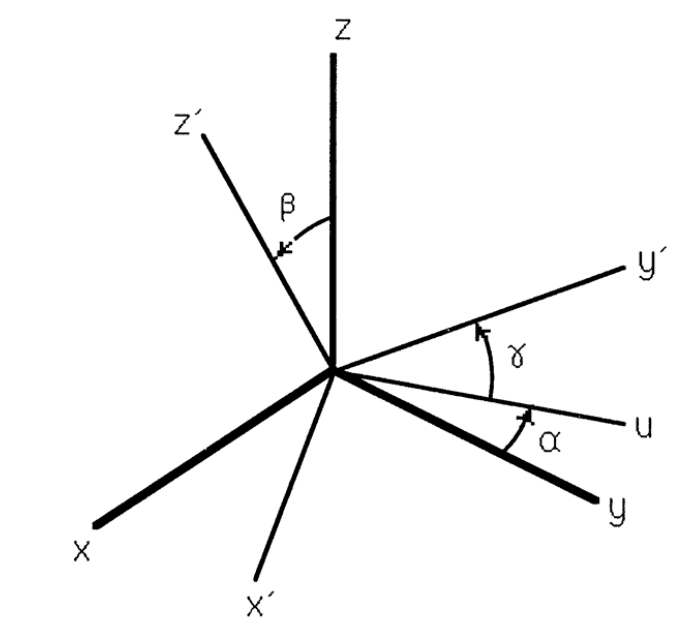
\includegraphics[height=4.5cm ,width=5cm]{QM/rotation.png}
	\caption{Euler angles}
\end{figure}
The net rotation is
\[\bm{R}(\alpha,\beta,\gamma) = \bm{R}_{z'}(\gamma) \bm{R}_{u}(\beta) \bm{R}_{z}(\alpha) = e^{-i\gamma J_{z'}} e^{-i\beta J_{u}} e^{-i\alpha J_{z}}\]
Since $J_u = \bm{R}_z(\alpha) J_y \bm{R}_z(-\alpha)$, we have $\bm{R}_u(\beta) = \bm{R}_z(\alpha) \bm{R}_y(\beta) \bm{R}_z(-\alpha)$. Similarly, we can obtain $\bm{R}_{z'}(\gamma) = \bm{R}_{u}(\beta) \bm{R}_z(\gamma) \bm{R}_u(-\beta)$. So, the rotation operator is
\[\bm{R}(\alpha,\beta,\gamma) = \bm{R}_{z}(\alpha) \bm{R}_{y}(\beta) \bm{R}_{z}(\gamma) = e^{-i\alpha J_{z}} e^{-i\beta J_{y}} e^{-i\gamma J_{z}}\]
The matrix representation of the rotation operator in the basis $|j,m\rangle$
\[\langle j',m' | \bm{R}(\alpha,\beta,\gamma) | j,m \rangle = \delta_{jj'} D_{m'm}^{(j)}(\alpha,\beta,\gamma)\]
gives rise to the rotation matrices,
\[D_{m'm}^{(j)}(\alpha,\beta,\gamma) = \langle j',m' | e^{-i\alpha J_{z}} e^{-i\beta J_{y}} e^{-i\gamma J_{z}} | j,m \rangle = e^{-i(\alpha m' + \gamma m)} d_{mm'}^{(j)}(\beta)\]
where
\[ d_{mm'}^{(j)}(\beta) = \langle j',m' | e^{-i\beta J_{y}} | j,m \rangle\]
For the case of $j = \frac{1}{2}$, we have $J_y = \frac{1}{2}\sigma_y$ and $\sigma_y^2 = I$. We can obtain
\[d^{(1/2)}(\beta) = \left[ \begin{matrix} \cos \frac{\beta}{2} & -\sin \frac{\beta}{2} \\ \cos \frac{\beta}{2}& \sin \frac{\beta}{2}\end{matrix} \right] \]
Notice that this matrix is periodic in $\beta$ with period $4\pi$, but it changes sign when $2\pi$ is added to $\beta$. This double-valuedness under rotation by $2\pi$ is a characteristic of the full rotation matrix whenever $j$ is a half odd-integer. The matrix is single-valued under rotation by $2\pi$ whenever $j$ is an integer.\\ \\
The operator for a rotation through $2\pi$ about an axis
along the unit vector $\bm{n}$ is $\bm{R}_n(2\pi) = e^{-2\pi i\bm{n}\cdot\bm{J}}$. Its effect on the standard angular momentum eigenvectors is
\[\bm{R}_n(2\pi) = (-1)^{2j}|j,m\rangle \]
We assume a rotation through $2\pi$ as a trivial operation that leaves everything unchanged, i.e. all dynamical variables are invariant under $2\pi$ rotation:
\[\bm{R}(2\pi) A \bm{R}^{-1}(2\pi) = A\]
where $A$ may represent any physical observable. \\
the operator $\bm{R}_{2\pi}$ divides the vector space into two subspaces. A typical vector in the first subspace,
denoted as $|+\rangle$, has the property $\bm{R}(2\pi)|+\rangle = |+\rangle$, whereas a typical vector in the second subspace, denoted as $|-\rangle$, has the property $\bm{R}(2\pi)|-\rangle = -|-\rangle$. Now, if $A$ represents any physical observable, we have $\langle + | \bm{R}(2\pi) A| - \rangle = \langle + | A\bm{R}(2\pi)| - \rangle$, leading to 
\[\langle + | A | - \rangle = 0\] 
No physical observable can have nonvanishing matrix elements between states with integer angular momentum and states with half odd-integer angular momentum. This fact forms the basis of a superselection rule: There is no observable distinction among the state vectors of the form\\
\[|\Psi_{\omega}\rangle = |+\rangle + e^{i\omega}|-\rangle\]
for different values of the phase $\omega$.

\section{Addition of angular momentum}
Let us consider a two-component system, each component of which has angular momentum degrees of freedom. Basis vectors for the composite system can be formed from the basis vectors of the components by taking all binary products of a vector from each set
\[|j_1,j_2,m_1,m_2\rangle = |j_1,m_1\rangle ^{(1)} |j_2,m_2\rangle ^{(2)}\]
These vectors are common eigenvectors of the four commutative operators $\bm{J}^{(1)}\cdot\bm{J}^{(1)}$, $\bm{J}^{(2)}\cdot\bm{J}^{(2)}$, $\bm{J}_z^{(1)}$, and $\bm{J}_z^{(2)}$.
It is often desirable to form eigenvectors of the total angular momentum operators, $\bm{J}\cdot\bm{J}$ and $\bm{J}_z$, where the total angular momentum vector operator is
\[\bm{J} = \bm{J}^{(1)}\otimes\bm{1} + \bm{1}\otimes\bm{J}^{(2)}\]
This is useful when the system is invariant under rotation as a whole, but not under rotation of the two components separately. 
The eigenvectors of $\bm{J}\cdot\bm{J}$ and $\bm{J}_z$ may be denoted as $|\alpha, J, M \rangle$. It is easy to verify that the four operators $\bm{J}^{(1)}\cdot\bm{J}^{(1)}$, $\bm{J}^{(2)}\cdot\bm{J}^{(2)}$, $\bm{J}\cdot\bm{J}$ and $\bm{J}_z$ are mutually commutative, and hence they possess a complete set of common eigenvectors. 
Since the set of product vectors and the new set of total angular momentum eigenvectors are both eigenvectors of $\bm{J}^{(1)}\cdot\bm{J}^{(1)}$ and $\bm{J}^{(2)}\cdot\bm{J}^{(2)}$, the eigenvalues $j_1$ and $j_2$ will be constant in both sets. Therefore
we may confine our attention to the vector space of dimension $(2j_1+1)(2j_2+1)$ that is spanned by product vectors with fixed values of $j_1$ and $j_2$.\\
Now the $2J+1$ vectors $|\alpha, J, M \rangle$, with $M$ in the range $-J \leq M \leq J$, span an irreducible subspace.
Therefore if the vector $|\alpha, J, M \rangle$, for a particular value of $M$, can be constructed in the space under consideration, then so can the entire set of $2J+1$
such vectors with $M$ in the range $-J \leq M \leq J$.
For a particular value of $J$, it might be possible to construct one such set of vectors, two or more linearly independent sets, or none at all. \\
Let $N(J)$ denote the number of independent sets that can be constructed. Let $n(M)$ be the degree of degeneracy, in this space, of the eigenvalue $M$ . The relation between these two quantities is
\[n(M) = \sum_{J \geq |M|} N(J)\]
and hence
\[N(J) = n(J) - n(J+1)\]
The product vectors $|j_1,m_1\rangle |j_2,m_2\rangle$ are eigenvectors of the operator $\bm{J}_z$, with eigenvalue $m_1+m_2$, and the degree of degeneracy $n(M)$ is equal to the number of pairs $(m_1,m_2)$ such that $M=m_1+m_2$.
\begin{figure}[!h]
	\centering
	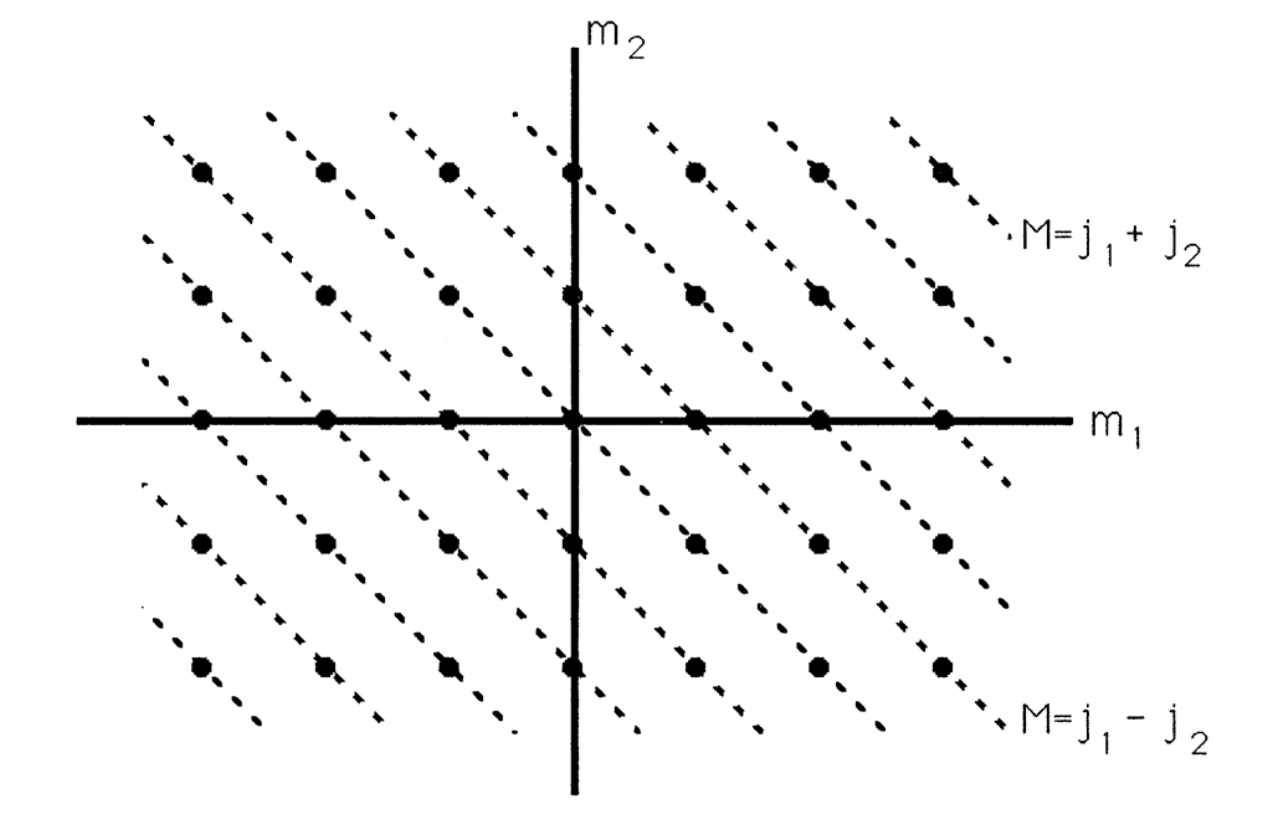
\includegraphics[height=4.14cm ,width=6.4cm]{QM/angular_momentum.png}
	\caption{Possible values of $M=m_1+m_2$ , illustrated for $j_1=3$, $j_2=2$}
\end{figure}
Therefore,
\[n(M)=\begin{cases} 0 \quad |M| > j_1 + j_2\\ j_1+j_2+1-|M|\quad |j_1-j_2| \leq M \leq |j_1+j_2|\\ 2j_{min}+1 \quad 0 \leq |M|\leq |j_1-j_2|\end{cases} \]
It then follows that
\[N(J)=\begin{cases} 1 \quad |j_1-j_2| \leq J \leq |j_1+j_2|\\ 0 \quad \mbox{otherwise}\end{cases} \]
It has turned out that $N(J)$ is never greater that $1$, and so the vectors $|\alpha, J, M \rangle$ can be uniquely labeled by the eigenvalues of the four operators $\bm{J}^{(1)}\cdot\bm{J}^{(1)}$, $\bm{J}^{(2)}\cdot\bm{J}^{(2)}$, $\bm{J}\cdot\bm{J}$ and $\bm{J}_z$. Henceforth these total angular momentum
eigenvectors will be denoted as $|j_1,j_2,J,M\rangle$. And we have the unitarity transformation 
\[|j_1,j_2,J,M\rangle = \sum_{m_1,m_2} |j_1,j_2,m_1,m_2\rangle \langle j_1,j_2,m_1,m_2 | j_1,j_2,J,M\rangle\]
The coefficients of this transformation are called the Clebsch–Gordan coefficients, denoted as $(j_1,j_2,m_1,m_2|J,M)$. We fix the phase of $|j_1, j_2, J, M\rangle$ by requiring that $(j_1,j_2,m_1,m_2|J,M)$ be real and positive. The CG coefficient vanishes unless the following conditions are satisfied:
\begin{itemize}
\item $m_1+m_2=M$
\item $|j_1-j_2| \leq J \leq |j_1+j_2|$
\item $j_1+j_2+J =$ an integer
\end{itemize}
It is possible to calculate the values of the CG coefficients by successive application of the raising or lowering operator to
\[|j_1,j_2,J,M\rangle = \sum_{m_1,m_2} |j_1,j_2,m_1,m_2\rangle \langle j_1,j_2,m_1,m_2 | j_1,j_2,J,M\rangle\]
The details of the calculation can be found in section 7.7 of \emph{Quantum mechanics - a modern development(Leslie E. Ballentine)}.And we have \href{https://en.wikipedia.org/wiki/Table_of_Clebsch-Gordan_coefficients}{Table of CG coefficients} and \href{http://www.wolframalpha.com/input/?i=CG+coefficient}{Calculator of CG coefficients} on the internet. A special case of angular momentum addition is spin–orbit coupling of spin $\frac{1}{2}$ particles, and we list the corresponding CG coefficients $(l,\frac{1}{2}, M-m_s, m_s|J,M)$ here:
\begin{table}[!th]
\begin{tabular}{|c|c|c|}
\hline
 & $J=l+\frac{1}{2}$ & $J=l-\frac{1}{2}$ \\
 \hline
 $m_s = \frac{1}{2}$ & $\left[ \frac{l+M+\frac{1}{2}}{2l+1}\right ]^{\frac{1}{2}} $ & $-\left[ \frac{l-M+\frac{1}{2}}{2l+1}\right ]^{\frac{1}{2}} $ \\
 \hline
 $m_s = -\frac{1}{2}$ & $\left[ \frac{l-M+\frac{1}{2}}{2l+1}\right ]^{\frac{1}{2}} $ & $\left[ \frac{l+M+\frac{1}{2}}{2l+1}\right ]^{\frac{1}{2}} $ \\
\hline
\end{tabular}
\caption{Spin-Orbit coupling}
\end{table}
\subsubsection{Magnetic moment}
The magnetic moment operator for an atom has the form
\[\bm{\mu} = \frac{-e}{2m_e c} (g_L\bm{L} + g_s \bm{S})\]
The parameters $g_L$ and $g_S$ have approximately the
values $g_L = 1$ and $g_S = 2$. The former is an generalization of the magnetic moment we calculated in classical electrodynamics for a system of charged particles. The latter will be discussed in quantum field theory. We define the effective Lande factor as
\[\langle \tau,J,M' | \bm{\mu} | \tau,J,M \rangle = \frac{-e}{2m_e c} g_{eff} \langle J,M' | \bm{J} | J,M \rangle\]
So, we have
\[g_{eff} = \frac{\langle \tau,J,M | g_L\bm{L}\cdot\bm{J} + g_s \bm{S}\cdot\bm{J} | \tau,J,M \rangle}{J(J+1)} = 1 + \frac{J(J+1)- L(L+1) + S(S+1)}{2J(J+1)}\]
A formal discussion can be found in section 7.8 of \emph{Quantum mechanics - a modern development(Leslie E. Ballentine)}.

\section{Spherical potential well}
The stationary states of a particle in the spherical potential well are determined by
\[-\frac{1}{2M}\nabla^2 \Psi  + W(r) \Psi = E\Psi \]
In spherical coordinates, 
\[\nabla^2 = \frac{1}{r^2} \frac{\partial}{\partial r} \left [ r^2\frac{\partial}{\partial r} \right ] + \frac{1}{r^2\sin\theta} \frac{\partial}{\partial \theta} \left [\sin\theta \frac{\partial}{\partial \theta} \right ] + \frac{1}{r^2\sin^2\theta} \frac{\partial^2}{\partial\phi^2}\]
So, the eigenvalue equation becomes
\[-\frac{1}{2M} \frac{1}{r^2} \frac{\partial}{\partial r} \left [ r^2\frac{\partial \Psi}{\partial r}\right ]  + \frac{L^2}{2Mr^2} \Psi + W(r)\Psi = E\Psi\]
Suppose the eigenfunctions have the factored form
\[\Psi(r,\theta,\phi) = Y_l^m(\theta,\phi) \frac{u(r)}{r}\]
The radial function then satisfies the equation
\[-\frac{1}{2M} \frac{d^2 u(r)}{dr^2} + \left[ \frac{l(l+1)}{2Mr^2} + W(r)\right]u(r) = Eu(r)\]
The radial function must satisfy the boundary condition $u(0) = 0$ since $\Psi(r,\theta,\phi)$ would otherwise have an $r^{-1}$ singularity at the origin. The normalization $\langle \Psi | \Psi \rangle = 1$ implies that
\[\int_0^{\infty} = |u(r)|^2 dr = 1\]

\subsubsection{The hydrogen atom}
The hydrogen atom is a two-particle system consisting of an electron and a proton. The Hamiltonian is
\[H = \frac{P_e^2}{2M_e} + \frac{P_p^2}{2M_p} - \frac{e^2}{4\pi|\bm{Q}_e-\bm{Q}_p|}\]
We take as independent variables the center of mass and relative coordinates of the particles
\[\bm{Q}_c = \frac{M_e\bm{Q}_e + M_p\bm{Q}_p}{M_e+M_p} \quad \bm{Q}_r = \bm{Q}_e-\bm{Q}_p\]
The corresponding momentum operators are
\[\bm{P}_c = \bm{P}_e + \bm{P}_p \quad \bm{P}_r = \frac{M_p\bm{P}_e-M_e\bm{P}_p}{M_e + M_p}\]
We can verify that
\[[Q_{c\alpha},P_{c\beta}] = [Q_{r\alpha},P_{r\beta}] = i\delta_{\alpha\beta} \quad [Q_{c\alpha},P_{r\beta}] = [Q_{r\alpha},P_{c\beta}] = 0\]
The Hamiltonian becomes
\[H = \frac{P_c^2}{2(M_e+M_p)} + \frac{p_r^2}{2\mu} - \frac{e^2}{4\pi|\bm{Q}_r|}\]
where $\mu$ is called the reduced mass, and is defined by $\mu \equiv \frac{M_eM_p}{M_e+M_p}$.
The center of mass behaves as a free particle, and its
motion is not coupled to the relative coordinate. We shall confine our attention to the internal degrees of freedom described by the relative coordinate $\bm{Q}_r$. The energy eigenvalue equation in coordinate representation is
\[-\frac{1}{2\mu}\nabla^2 \Psi(\bm{r})  -\frac{e^2}{4\pi r} \Psi(\bm{r}) = E\Psi(\bm{r})\]
Suppose $\Psi(r,\theta,\phi) = Y_l^m(\theta,\phi) \frac{u(r)}{r}$, we have
\[-\frac{1}{2\mu} \frac{d^2 u(r)}{dr^2} + \left[ \frac{l(l+1)}{2\mu r^2} - \frac{e^2}{4\pi r}\right]u(r) = Eu(r)\]
Define
\[\rho \equiv \alpha r \quad \alpha \equiv \sqrt{8\mu|E|} \quad \lambda \equiv \frac{e^2}{4\pi} \sqrt{\frac{\mu}{2|E|}}\]
we have
\[\frac{d^2 u}{d\rho^2} + \left[ -\frac{1}{4} + \frac{\lambda}{\rho} - \frac{l(l+1)}{\rho^2} \right] u = 0\]
As $\rho \to \infty$, we have $u \sim e^{-\rho/2}$. And as $\rho \to 0$, we have $u \sim \rho^{l+1}$. So, we can suppose
\[u(\rho) = \rho^{l+1} e^{-\rho/2} v(\rho)\]
And we can get
\[\rho \frac{d^2 v}{d\rho^2} + (2l+2-\rho)\frac{dv}{d\rho} + (\lambda-l-1)v = 0\]
It is the so-called \href{http://mathworld.wolfram.com/ConfluentHypergeometricDifferentialEquation.html}{Confluent Hypergeometric Differential Equation}.
When $\lambda - 1- l = n_r$, we have regular solutions. Solutions are \href{https://en.wikipedia.org/wiki/Laguerre_polynomials#Generalized_Laguerre_polynomials}{Associated Laguerre Polynomial}, and will be denoted as $L_{n-l-1}^{2l+1}(\rho) (n=n_r+l+1)$. The energy levels are
\[E_n = -\frac{\mu e^4}{32\pi^2 n^2}\]
The degeneracy of an eigenvalue $E_n$ is
\[\sum_{l=0}^{n-1} (2l+1) = n^2\]
\begin{note}
The degeneracy of an energy level of a hydrogen atom is greater than this by a factor of $4$, which arises from the two-fold orientational degeneracies of the electron and proton spin states. This four-fold degeneracy is modified by the hyperfine interaction between the magnetic moments of the electron and the proton.
\end{note}
The orthonormal energy eigenfunctions for the hydrogen atom are
\[\Psi_{nlm}(r,\theta,\phi) =  \left[ \frac{4(n-l-1)!}{(na_0)^3 n[(n+l)!]^3} \right]^{\frac{1}{2}} \rho^l L_{n-l-1}^{2l+1}(\rho) e^{-\rho/2} Y_l^m (\theta,\phi)\]
where $\rho = \alpha r = \frac{2r}{na_0}$, and $a_0 \equiv \frac{4\pi}{\mu e^2}$ is a characteristic length for the
atom, known as the Bohr radius.The ground state wave
function is
\[\Psi_{000} = (\pi a_0^3)^{-\frac{1}{2}} e^{-\frac{r}{a_0}}\]
A measure of the spatial extent of the bound states of hydrogen is given by the averages of various powers of the distance $r$.
\begin{eqnarray}
\langle r \rangle &=& n^2a_0 \left \{ 1 + \frac{1}{2} \left [ 1 - \frac{l(l+1)}{n^2} \right] \right\} \nonumber \\
\langle r^2 \rangle &=& n^4a_0^2 \left \{ 1 + \frac{3}{2} \left [ 1 - \frac{l(l+1)-1/3}{n^2} \right] \right\} \nonumber \\
\langle \frac{1}{r} \rangle &=& \frac{1}{n^2 a_0} \nonumber
\end{eqnarray}

\chapter{Quantum-mechanical Particles and Classical Electromagnetic Field}
\section{Charged Particle in EM field}
In classical electrodynamics, if the velocity of the charged particle is much smaller than that of light, then the Hamiltonian of charged particles in a given EM field is
\[H = \frac{(\bm{\pi}-e\bm{A})^2}{2m} + e\phi\]
In corresponding quantum theory, we will suppose the Hamiltonian operator to be
\[H = \frac{[\bm{P}-e\bm{A}(\bm{X})]^2}{2M} + e\phi(\bm{X})\]
The corresponding field operators are
\[\bm{E} = -\nabla\phi - \frac{\partial \bm{A}}{\partial t} \quad \bm{B} = \bm{\nabla}\times\bm{A}\]\\
In Heisenberg picture, we have
\[\frac{d\bm{X}}{dt} = -i[\bm{X},H] = \frac{1}{M}(\bm{P}-e\bm{A})\]
Define kinetic momentum $\bm{K}$ by
\[\bm{K} = \bm{P}-e\bm{A}\]
We have
\[[K_i,K_j] = ie(\partial_i A_j-\partial_j A_i) = ie\epsilon_{ijk}B_k\]
So
\[M \frac{d^2\bm{X}}{dt^2} = -i[\bm{K},H] + \frac{\partial \bm{K}}{\partial t} = e \left[ \bm{E}+ \frac{1}{2} \left( \frac{d\bm{X}}{dt} \times \bm{B} - \bm{B}\times\frac{d\bm{X}}{dt} \right) \right]\]\\
In coordinate representation of Schrödinger picture, we have
\[\frac{1}{2M} \left[ -i\bm{\nabla}-e\bm{A} \right] \cdot \left[ -i\bm{\nabla}-e\bm{A} \right] \psi(\bm{x},t) + e\phi(\bm{x})\psi(\bm{x},t) = i \frac{\partial \psi(\bm{x},t)}{\partial t}\]
Define probability current $\bm{j}$ as
\[\bm{j} \equiv \frac{1}{M} \mathrm{Im}(\psi^{*}\bm{\nabla}\psi) - \frac{e}{M}\bm{A}|\psi|^2\]
we can verify that
\[\bm{\nabla}\cdot\bm{j} + \frac{\partial \rho}{\partial t} = 0\]\\
Transformation
\[\phi \to \phi - \frac{\partial \Lambda}{\partial t} \quad \bm{A} \to \bm{A} + \bm{\nabla}\Lambda\]
will leave $\bm{E}$ and $\bm{B}$ unchanged. The transformation is called gauged transformation. In classical electrodynamics, gauge transformation will not change the trajectory of particles, (which is the only thing we can observed in experiment). In quantum theory, suppose the state vector $|\psi\rangle$ will transform as 
\[|\psi(t)\rangle \to O(t)|\psi(t)\rangle\]
where $O(t)$ is an unitary operator. If the Schrödinger equation is always satisfied, we can derive that
\[H'O - OH = i\frac{\partial O}{\partial t}\]
where $H'$ is the Hamiltonian operator after gauge transformation. Generally, we have
\[O(t) = \exp \left[ ie\Lambda(\bm{X},t)\right]\]
And so
\[O^{-1} \bm{X} O = \bm{X} \quad O^{-1} \bm{P} O = \bm{P} + e\bm{\nabla}\Lambda \quad O^{-1}(\bm{P}-e\bm{A}')O = \bm{P} - e\bm{A}\]
So, the expectation value of $\bm{X}$ and $\bm{K}$ is invariant under gauge transformation. We can also verify that $\bm{j}$ is also invariant under gauge transformation.
A special case is that
\[\phi \to \phi+\phi_0(t) \quad \bm{A} \to \bm{A}\]
In this case, we have
\[O(t) = \exp \left[ -i \int_{t_0}^{t} dt' e\phi_0(t') \right]\]
If $\phi_0$ is a constant, then
\[O(t) = \exp \left[ -ie\phi_0(t-t_0) \right]\]

\section{Charged particle in a magnetic field}
\subsection{Motion in a uniform static magnetic field} 
Suppose that the magnetic field be of magnitude $B$ in the $z$ direction. The Hamiltonian $H = H_{xy}+H_z$ with $H_{xy} = \frac{K_x^2+K_y^2}{2M}$ and $H_z = \frac{P_z^2}{2M}$. Since $B_x = B_y = 0$ , then $P_z$ commutes with $P_x$ and $P_y$. Hence the operators $H_{xy}$ and $H_z$ are commutative, and every eigenvalue of $H$ is just
the sum of an eigenvalue of $H_{xy}$ and an eigenvalue of $H_z$. \\
Define
\[Q' \equiv \frac{K_x}{\gamma} \quad P' \equiv \frac{K_y}{\gamma} \quad \gamma \equiv \sqrt{|eB|} \]
Then we have
\[H_{xy} = \frac{1}{2} \frac{|eB|}{M}(Q'^2+P'^2) \mbox{  with  } [Q',P'] = i \mbox{  or  }-i\]
therefore the eigenvalues of $H_{xy}$ must be equal to $(n+\frac{1}{2})\frac{|eB|}{M}$, where $n$ is any non-negative integer.\\
The spectrum of $K_z$ can be shown to be gauge-invariant.
Because the magnetic field is uniform and in the $z$ direction, it is possible to choose the vector potential such that $A_z = 0$. Therefore the spectrum of $K_z$ is
continuous from $-\infty$ to $\infty$, like that of $P_z$.\\
Thus the energy eigenvalues for a charged particle in a uniform static magnetic field $B$ are
\[E_n(p_z) = \frac{(n+\frac{1}{2})|eB|}{M} + \frac{p_z^2}{2M}\]
The motion parallel to the magnetic field is not coupled to the transverse motion, and is unaffected by the field. The classical motion in the plane perpendicular to the field is
in a circular orbit with angular frequency $\omega_c = \frac{eB}{M}$, and it is well known that periodic motions correspond to discrete energy levels whose separation is $\omega_c$.\\ \\
Now let us choose the vector potential to be $A_x=-yB$,$A_y=A_z=0$. The Hamiltonian now becomes
\[H = \frac{(P_x+yeB)^2 + P_y^2 + P_z^2}{2M}\]
$P_x$ and $P_z$ commute with $H$, so it is possible to construct a complete set of common eigenvectors of $H$, $P_x$ and $P_z$. In coordinate representation, the eigenvalue equation now takes the form
\[-\frac{1}{2M}\nabla^2 \psi - \frac{ieB}{M}y\frac{\partial}{\partial x}\psi + \frac{e^2B^2}{2M}y^2\psi = E\psi\]
Substitute
\[\psi(x,y,z) = \exp(ik_xx+ik_zz)\phi(y)\]
The equation then takes the form
\[-\frac{1}{2M} \frac{d^2\phi(y)}{dy^2} + \left[ \frac{M\omega_c^2}{2}(y-y_0)^2-E' \right]\phi(y) = 0\]
where $\omega_c = \frac{eB}{M}$ is the classical cyclotron frequency, and $E'=E-\frac{k_z^2}{2M}$ is the energy associated with motion in the $xy$ plane. This is just the energy eigenvalue equation for a simple harmonic oscillator with angular frequency $\omega = |\omega_c|$, whose eigenvalues are $E' = (n+1/2)\omega$. Thus the energies for the charged particle in the magnetic field must be $E = (n+1/2)|\omega_c|+\frac{k_z^2}{2M}$. Apart from a normalization constant, the eigenfunction will be
\[\psi = \exp(ik_xx+ik_zz) H_n[\alpha(y-y_0)]\exp[-\frac{1}{2}\alpha^2 (y-y_0)^2]\]
with $\alpha = \sqrt{M\omega} = \sqrt{|eB|}$, and $y_0 = - \frac{k_x}{eB}$.\\
For fixed $n$ and $k_z$, the energy eigenvalue is highly degenerate. For convenience, we assume that the system is confined to a rectangle of dimension $D_x\times D_y$ and subject to periodic boundary conditions. The allowed
values of $k_x$ are $k_x = \frac{2\pi n_x}{D_x}$, with $n_x = 0,\pm1,\cdots$.The orbit center coordinate $y_0 = -\frac{2\pi n_x}{D_xeB}$ must lie in the range $[0,D_y]$. In the limit as $D_x$ and $D_y$ become large, we may ignore problems associated with orbits lying near the boundary, since they will be a negligible fraction of the total. In this limit the number of degenerate states corresponding to fixed $n$ and $k_z$ will be $\frac{D_xD_y |eB|}{2\pi}$.

\subsection{The Aharonov-Bohm effect}
A long solenoid is placed perpendicular to the plane of the figure, so that a magnetic field can be created inside the solenoid while the region external to the solenoid remains field-free. The solenoid is located in the unilluminated shadow region so that no particles will reach it, and moreover it may be surrounded by a cylindrical shield that is impenetrable to the charged particles. Nevertheless it can be shown that the interference pattern depends upon the magnetic flux through the cylinder.\\
\begin{figure}[!h]
	\centering
	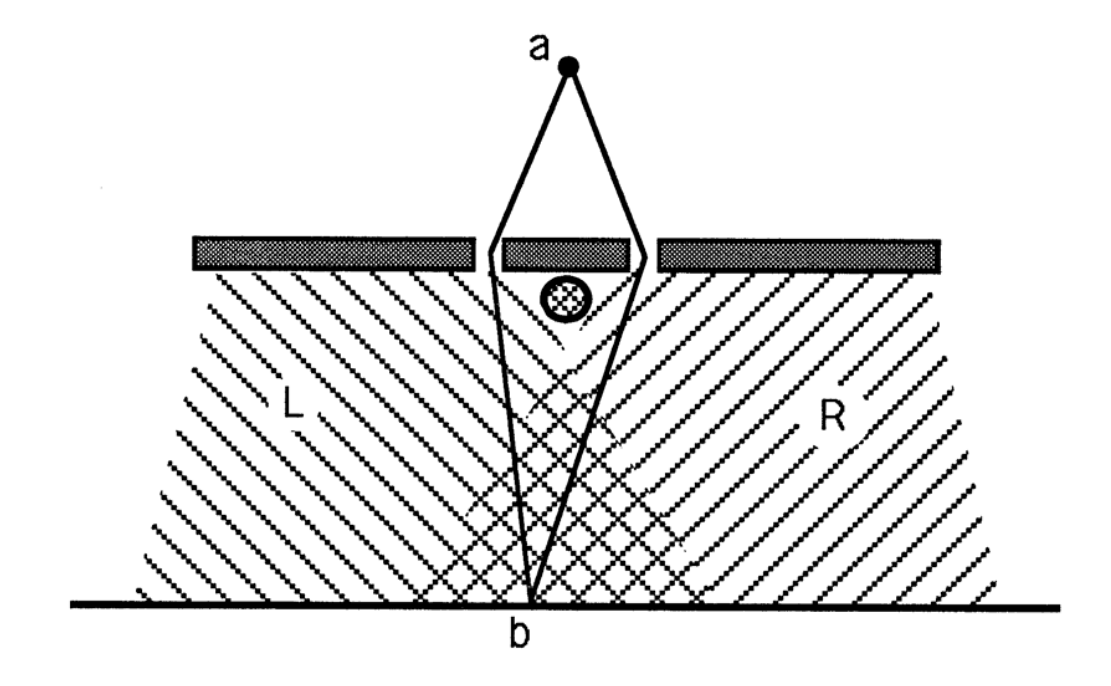
\includegraphics[height=4cm ,width=6.5cm]{QM/AB_effect.png}
	\caption{The Aharonov–Bohm experiment}
\end{figure}\\
Let $\Psi^{(0)}(\bm{x},t)$ be the solution of the Schrödinger equation and boundary conditions of this problem for the case in which the vector potential is everywhere zero. Now let us consider the case in which the magnetic field is non-zero inside the cylinder but zero outside of it. The vector potential $\bm{A}$ will not vanish everywhere in the exterior region, even though $\bm{B}=\bm{\nabla}\times\bm{A}=0$
outside of the cylinder. This follows by applying Stokes's theorem to any path surrounding the cylinder
\[\oint \bm{A}\cdot d\bm{x} = \int\int (\bm{\nabla}\times\bm{A})\cdot d\bm{S} = \int\int \bm{B}\cdot d\bm{S} = \Phi\]
If the flux through the cylinder is not zero, then the vector potential must be nonzero on every path that encloses the cylinder. However in any simply connected region outside of the cylinder, it is possible to express the vector potential as the gradient of a scalar, from the zero potential solution by means of a gauge transformation, $\Psi = \Psi^{(0)}\exp(ie\Lambda)$.\\
In region $L$, which contains the slit on the left, the wave function can be written as $\Psi_L = \Psi_L\exp(ie\Lambda_1)$, where $\Psi_L$ is the zero potential solution in region $L$, and $\Lambda_1(\bm{x},t) = \int \bm{A}\cdot d\bm{x}$, with the integral taken along a path within region L. A similar form can be written for the wave function in the region R, which contains the slit on the right. \\
At the point b, in the overlap of regions L and R, the wave function is a superposition of contributions from both slits. Hence we have
\[\Psi(\bm{b}) = \Psi_L\exp(ie\Lambda_1) + \Psi_R\exp(ie\Lambda_2)\]
The interference pattern depends $\exp(ie(\Lambda1-\Lambda_2)) = \exp(ie\Phi)$. 
Therefore the interference pattern is sensitive to the magnetic flux inside of the cylinder, even though the particles never pass through the region in which the magnetic field is nonzero. 
The AB effect is a topological effect, in that the effect depends on the flux encircled by the paths available to the particle, even though the paths may never approach the region of the flux. \\
At last, we conclude that in quantum theory, the potentials themselves are physically significant; however, they are subject to the requirement that all observable effects be invariant under gauge transformations.

\subsection{The Zeeman effect}
The Zeeman effect refers to the effect of a uniform magnetic field on atomic states and energy levels.
The Hamiltonian for an electron in the atom is
\[H = \frac{(\bm{P}+e\bm{A})^2}{2M} + W(r) = \frac{P^2}{2M} + \frac{e}{M}\bm{A}\cdot\bm{P} + \frac{e^2A^2}{2M} + W(r)\]
where the mass of the electron is $M$, and its charge is $-e$. We have used the simplification $\bm{P}\cdot\bm{A} = \bm{A}\cdot\bm{P}$, which is valid if $\bm{\nabla}\cdot\bm{A}=0$. 
We shall take vector potential to be $\bm{A}(\bm{X}) = \frac{1}{2}\bm{B}\times\bm{X}$. It then follows that
\[\bm{A}\cdot\bm{P} = \frac{1}{2}(\bm{B}\times\bm{X})\cdot\bm{P} = \frac{1}{2}(\bm{X}\times\bm{P})\cdot\bm{B} = \frac{1}{2} \bm{B}\cdot\bm{L}\]
For weak magnetic fields it is convenient to write this Hamiltonian in the form
\[H = H_a + \frac{e}{2M} \bm{B}\cdot\bm{L} + \frac{e^2}{8M}(\bm{B}\times\bm{X})^2\]
where $H_a = \frac{P^2}{2M} + W(r)$ is the Hamiltonian of the free atom.
If we neglect the last term of $H$, which is of the second order in the magnetic field, and choose the magnetic field to lie along the z axis, then eigenfunctions $\Psi_{nlm}$ of $H_a$ will also be an eigenfunction of $H$. To the first order in the magnetic field, the atomic energy levels will be displaced by an amount
\[E^{(1)} = \frac{eB}{2M}m\]
The degeneracy of the $2l+1$ fold multiplet of fixed $n$ and $l$, due to the spherical symmetry of the atom, is broken by the magnetic field.
\begin{note}
There is also a magnetic dipole moment associated with the spin, $\bm{\mu}_{S} = -\frac{e}{M}\bm{S}$, and so in practice one must also add the spin term $-\bm{\mu}_{S} \cdot \bm{B}$ to the Hamiltonian.
\end{note}
For strong magnetic fields the term in the Hamiltonian that is proportional to $B^2$ becomes important. The details of the discussion can be found in section 11.5 of \emph{Quantum mechanics - a modern development(Leslie E. Ballentine)}.

\chapter{Discrete Symmetries}
\section{Space inversion}
The space inversion transformation is $\bm{x} \to -\bm{x}$. The corresponding operator on state vector space is usually called the parity operator. It will be denoted by $P$. By definition, the parity operator reverses the signs of the position operator and the momentum operator
\[P^{-1}\bm{X}P = -\bm{X} \quad P^{-1}\bm{P}P = -\bm{P}\]
It follows that the orbital angular momentum, $\bm{L} = \bm{X}\times\bm{P}$, is unchanged by the parity transformation. This property is extended, by definition, to any angular momentum operator,
\[P^{-1}\bm{J}P = \bm{J}\]
We can verify that $P$ must be linear by applying space inversion to the commutation relation $[X_i,P_i] = i$. Therefore the parity operator is a unitary operator rather than an anti-unitary operator. Since two consecutive space inversions produce no change at all, it follows that the states described by $|\psi\rangle$ and by $P^2|\psi\rangle$ must be the same. Thus the
operator $P^2$ can differ from the identity operator by at most a phase factor. This phase factor is left arbitrary. It is most convenient to choose that phase factor to be unity, and hence we have
\[P = P^{-1} = P^{\dagger}\]
Further more, we can derive that
\[P|\bm{x}\rangle = |-\bm{x}\rangle\]
So the effect of $P$ on a wave function is
\[P\psi(\bm{x}) \equiv \langle \bm{x} | P | \psi\rangle = \langle -\bm{x} | \psi\rangle = \psi(-\bm{x})\]
From the fact the $P^2=1$, it follows that $P$ has eigenvalues $\pm 1$. Any even function, $\psi_e(\bm{x}) = \psi_e(-\bm{x})$, is an eigenfunction on $P$ with eigenvalue $1$, and any odd function, $\psi_o(\bm{x}) = -\psi_o(-\bm{x})$, is an eigenfunction of $P$ with eigenvalue $-1$.
A function corresponding to parity $+1$ is also said to be of even parity, and a function corresponding to parity $-1$ is said to be of odd parity.\\ \\
\textbf{Example}\\
Under space inversion, $\bm{x} \to -\bm{x}$, the spherical harmonic undergoes the transformation
\[Y_l^m(\theta,\phi) \to Y_l^m(\pi-\theta,\phi+\pi) = (-1)^l Y_l^m(\theta,\phi)\]
Hence the single particle orbital angular momentum eigenvector $|l,m\rangle$ is also an eigenvector of parity, with parity $(-1)^l$.\\
A total orbital angular momentum eigenvector for a two-
electron atom is of the form
\[|l_1,l_2,L,M\rangle = \sum_{m_1,m_2}  \langle l_1,l_2,m_1,m_2 | l_1,l_2,L,M\rangle |l_1,m_1\rangle \otimes |l_2,m_2\rangle\]
It is apparent that
\[P|l_1,l_2,L,M\rangle = (-1)^{l_1+l_2}|l_1,l_2,L,M\rangle\]
and that $(-1)^{l_1+l_2} \neq (-1)^{L}$ . Thus we see that, in general, the parity of an angular momentum state is not determined by its total angular momentum.\\ \\
If the parity operator $P$ commutes with the Hamiltonian $H$, then parity eigenvalue $\pm 1$ is a conserved quantity. In that case an even parity state can never acquire an odd parity component, and an odd parity state can never acquire an even parity component. \\
If $|\psi(t)\rangle$ is a physical process of the system with Hamiltonian $H$, then we have Schrödinger equation 
\[H|\psi\rangle = i\frac{\partial |\psi\rangle }{\partial t}\]
If $PH = HP$, we can verify that
\[H P|\psi\rangle = i\frac{\partial P |\psi\rangle }{\partial t}\]
So, the space inversion of $|\psi(t)\rangle$, $P|\psi(t)\rangle$, can also be a possible physical process of the system.\\
Experiments have shown that parity in $\beta$ decay is not conserved.

\section{Time reversal}
The effect of the time reversal operator $T$ is to reverse the linear and angular momentum while leaving the position unchanged. Thus we require, by definition,
\[T^{-1}\bm{X}T = \bm{X} \quad T^{-1}\bm{P}T = -\bm{P} \quad T^{-1}\bm{J}T = -\bm{J}\]
We can verify that $T$ must be anti-linear by applying space inversion to the commutation relation $[X_i,P_i] = i$. Therefore the parity operator is a anti-unitary operator.\\
The time evolution of a system satisfied Schrödinger equation
\[H|\psi(t)\rangle = i\frac{\partial |\psi(t)\rangle }{\partial t}\]
Suppose that $TH=HT$, we can derive that
\[HT|\psi(t)\rangle = -i\frac{\partial T|\psi(t)\rangle }{\partial t}\]
i.e.
\[HT|\psi(-t)\rangle = i\frac{\partial T|\psi(-t)\rangle }{\partial t}\]
$T|\psi(-t)\rangle$ is also a possible physical process of the system.\\ \\
In coordinate representation the Schrödinger equation takes the form
\[ \left[ -\frac{1}{2M}\nabla^2 + W(\bm{x}) \right] \psi(\bm{x},t) = i\frac{\partial \psi(\bm{x},t)}{\partial t}\]
Its complex conjugate is
\[ \left[ -\frac{1}{2M}\nabla^2 + W^*(\bm{x}) \right] \psi^*(\bm{x},t) = -i\frac{\partial \psi^*(\bm{x},t)}{\partial t}\]
The condition for the Hamiltonian to be invariant under complex conjugation is that the potential be real: $W=W^*$. In that case it is apparent that if $\psi(\bm{x},t)$ is a solution then so is  $\psi^*(\bm{x},t)$. This suggests that we may identify the time reversal operator with the complex conjugation operator in this representation,
\[T = K_0\]
where, by definition, $K_0\psi(\bm{x},t) = \psi^*(\bm{x},t)$. In this case $T$ is its own inverse. 
The formal expression for an arbitrary vector in coordinate representation is $|\psi\rangle = \int \psi(\bm{x})|\bm{x}\rangle d^3 \bm{x}$, where the basis vector $|\bm{x}\rangle$ is an eigenvector of the position operator. Since $T$ is equal to the complex conjugation operator, its effect is simply $T|\psi\rangle = \int \psi^*(\bm{x})|\bm{x}\rangle d^3 \bm{x}$, with $T|\bm{x}\rangle = |\bm{x}\rangle$.\\ \\
In momentum representation, an arbitrary vector can be written as
\[|\psi\rangle = \int \psi(\bm{p})|\bm{p}\rangle d^3 \bm{p}\]
Since
\[T|\bm{p}\rangle = \int \langle \bm{x} | \bm{p}\rangle^* |
\bm{x}\rangle d^3 \bm{x} = |-\bm{p}\rangle\]
so we have
\[T|\psi\rangle = \int \psi^*(\bm{p})|-\bm{p}\rangle d^3 \bm{p} = \int \psi^*(\bm{-p})|\bm{p}\rangle d^3 \bm{p}\]\\ 
The time reversal operator must reverse the angular momentum. For spin operator, we have
\[T^{-1}\bm{S}T = -\bm{S}\]
In the standard representation of the spin operators, $S_x$ and $S_z$ are real, while $S_y$ is imaginary. The time reversal operator $T$ cannot be equal to the complex conjugation operator $K_0$ in this representation, since the effect of the latter is
\[K_0S_xK_0 = S_x \quad K_0S_yK_0 = -S_y \quad K_0S_zK_0 = S_z\]
Let us write the time reversal operator as $T=YK_0$, where $Y$ is a linear operator. $Y$ must have the following properties:
\[Y^{-1}S_xY = -S_x \quad Y^{-1}S_yY = S_y \quad Y^{-1}S_zY = -S_z\]
And $Y$ must operate only on the spin degrees of freedom. A reasonable choice is that $Y = e^{-i\pi S_y}$, whose effect is
to rotate spin (and only spin) through the angle $\pi$ about the $y$ axis. Therefore the explicit form of the time reversal in this representation is
\[T = e^{-i\pi S_y}K_0\]\\
Two successive applications of the time reversal transformation, must leave the physical situation unchanged. Therefore
\[T^2|\Psi\rangle = c|\Psi\rangle\]
where $|c|=1$. And we have
\[T^2(T|\Psi\rangle) = T(T^2|\Psi\rangle) = T(c|\Psi\rangle) = c^* T|\Psi\rangle\]
so 
\[T^2(|\Psi\rangle + T|\Psi\rangle) = c|\Psi\rangle + c^* T|\Psi\rangle = c'(|\Psi\rangle + T|\Psi\rangle)\]
And we can determine that $c' = c^* = c$. Thus we must have $c = \pm 1$, i.e.
\[T^2|\Psi\rangle = \pm |\Psi\rangle\]
In the particularly representation, we have
\[T^2 = e^{-i\pi S_y}K_0 e^{-i\pi S_y}K_0 = e^{-i2\pi S_y}\]
This may equivalently be written as
\[T^2 = e^{-i2\pi J_y}\]
since $e^{-i2\pi L_y} = I$. So we have an identity
\[T^2 = R(2\pi)\]

\subsubsection{Kramer's theorem}
Let us consider the energy eigenvalue equation, $H|\Psi\rangle = E|\Psi\rangle$, for a time-reversal-invariant Hamiltonian, $TH=HT$. 
Then $HT|\Psi\rangle =  TH|\Psi\rangle = ET|\Psi\rangle$, and so
both $|\Psi\rangle$ and $T|\Psi\rangle$ are eigenvectors with energy eigenvalue $E$. 
There are two possibilities: 
(a) $|\Psi\rangle$and $T|\Psi\rangle$ are linearly dependent, and so describe the same state.
(b) $|\Psi\rangle$and $T|\Psi\rangle$ are linearly independent,
and so describe two degenerate states.\\
Suppose that (a) is true, in which case we must have $T|\Psi\rangle = a|\Psi\rangle$ with $|a|=1$. A second application of T yields $T^2|\Psi\rangle = |\Psi\rangle$. 
So for those states that satisfy $T^2|\Psi\rangle = -|\Psi\rangle$ it is necessarily true that $|\Psi\rangle$and $T|\Psi\rangle$ are linearly independent, degenerate states. This result is known as Kramer's theorem: any
system for which $T^2|\Psi\rangle = -|\Psi\rangle$ has only degenerate energy levels.

\chapter{Approximation method}
\section{Time independent perturbation theory}
\section{Time dependent perturbation theory}
\section{Atomic Radiation}
\section{The classical limit}

\chapter{Many body problem}
\section{Identical particles}
\section{Non-relativistic quantum field theory}

\chapter{Scattering theory}
\section{Lippmann–Schwinger equation}
Imagine a particle coming in and getting scattered by a short-ranged potential $V(x)$ located around the origin $x \sim 0$. The time-independent Schr\"{o}dinger equation is simply
\[(H_0 + V)|\psi\rangle = E |\psi\rangle\]
Here, $H_0 = \frac{p^2}{2m}$ is the free-particle Hamiltonian operator. We can write the solution as
\[|\psi^{(\pm)}\rangle = \frac{1}{E-H_0 \pm i\epsilon}V|\psi^{(\pm)}\rangle + |\phi\rangle\]
Here, $H_0 |\phi\rangle = E |\phi\rangle$. In coordinate representation,
\[\psi^{(\pm)}(\mathbf{x}) = \phi(\mathbf{x}) + \int d^3x' \langle \mathbf{x} | \frac{1}{E-H_0 \pm i\epsilon} | \mathbf{x}' \rangle V(\mathbf{x}') \psi^{(\pm)}(\mathbf{x}')\]
Here, $\phi(\mathbf{x}) = \frac{e^{i\mathbf{k}\cdot\mathbf{x}}}{(2\pi)^{\frac{3}{2}}}$. Define the Green function as
\[G_{\pm}(\mathbf{x},\mathbf{x}') \equiv \frac{1}{2m} \langle \mathbf{x} | \frac{1}{E-H_0 \pm i\epsilon} | \mathbf{x}' \rangle\]
We can derive that
\[G_{\pm}(\mathbf{x},\mathbf{x}') = -\frac{1}{4\pi} \frac{e^{\pm ik|\mathbf{x}-\mathbf{x}'|}}{|\mathbf{x}-\mathbf{x}'|}\]
where $k = \sqrt{2mE}$. And it is easy to show that
\[(\nabla^2 + k^2)G_{\pm}(\mathbf{x},\mathbf{x}') = \delta(\mathbf{x}-\mathbf{x}')\]
So, we have
\[\psi^{(\pm)}(\mathbf{x}) = \frac{e^{i\mathbf{k}\cdot\mathbf{x}}}{(2\pi)^{\frac{3}{2}}} - 2m \int d^3x' \frac{1}{4\pi} \frac{e^{\pm ik|\mathbf{x}-\mathbf{x}'|}}{|\mathbf{x}-\mathbf{x}'|} V(\mathbf{x}') \psi^{(\pm)}(\mathbf{x}')\]
We now can interpret $\psi^{+}(\mathbf{x})$ as a superposition of incident plane wave and scattered wave which propagate from scatterer to outside region. From now on, we will denote it as $\psi(\mathbf{x})$.

The experiment is done typically by placing the detector far away from the scatterer $|\mathbf{x}| \ll a$ where $a$ is the "size" of the scatterer. The integration over $\mathbf{x}'$, on the other hand, is limited within the "size" of the scatterer because of the $V(\mathbf{x}')$ factor. Therefore, we are in the situation $|\mathbf{x}| \ll |\mathbf{x}'|$, and hence can use the approximation
\[|\mathbf{x}-\mathbf{x}'| \approx |\mathbf{x}| - \frac{\mathbf{x}' \cdot \mathbf{x}}{|\mathbf{x}|}\]
Under this limit,
\[\psi(\mathbf{x}) = \frac{e^{i\mathbf{k}\cdot\mathbf{x}}}{(2\pi)^{\frac{3}{2}}} - 2m \frac{e^{ikr}}{4\pi r} \int d^3x' e^{-\mathbf{k}' \cdot \mathbf{x}'} V(\mathbf{x}') \psi(\mathbf{x}')\]
Here, $r = |\mathbf{x}|$ and $\mathbf{k}' = k \frac{\mathbf{x}}{r}$. It is customary to write this equation in the form
\[\psi(\mathbf{x}) = \frac{1}{(2\pi)^{\frac{3}{2}}}\left( e^{i\mathbf{k}\cdot\mathbf{x}} +  f(\mathbf{k},\mathbf{k}') \frac{e^{ikr}}{r} \right) \]
Here,
\[f(\mathbf{k},\mathbf{k}') \equiv - \frac{m}{2\pi} (2\pi)^3  \langle \mathbf{k}'| V | \psi\rangle \]
Recall the definition of cross section
\[\sigma \equiv \frac{\mbox{Number of Events}}{\mbox{Time} \times \mbox{Incident Flux}}\]
So, the differential cross section for particles being scattered into the solid angle is
\[d\sigma = \frac{|\mathbf{j}_{\mathrm{scatt}}| r^2 d\Omega}{|\mathbf{j}_{\mathrm{inc}}|} = |f(\mathbf{k},\mathbf{k}')|^2 d\Omega\]

In a more realistic situation, we should use wave packets to describe the scattering process. The basic picture is a free wave packet approaches the scattering center. After a long time, we have both the original wave packet moving in the original direction plus a spherical wave front that moves outward. The details can be found in the section 3 of the lecture notes 
\href{http://hitoshi.berkeley.edu/221B/index.html}{\emph{Scattering Theory I (Hitoshi Murayama)}}.

Furthermore, if we require that the normalization of the wave function should always satisfy $\int dx^3 |\psi(\mathbf{x})|^2$ for any $t$, as guaranteed by the unitarity of time evolution operator. This requirement leads to a special requirement on the scattered wave, and hence $f(\mathbf{k},\mathbf{k}')$, from witch we can derive the optical theorem.

\begin{newthem}[Optical theorem]
\[\mathrm{Im} f(\theta = 0) = \frac{k\sigma_{\mathrm{tot}}}{4\pi}\]
where
\[f(\theta = 0) \equiv f(\mathbf{k},\mathbf{k}),\]
the setting of $\mathbf{k} \equiv \mathbf{k}'$ imposes scattering in the forward direction, and
\[\sigma_{\mathrm{tot}} = \int \frac{d\sigma}{d\Omega} d\Omega\]
\end{newthem}
The meaning of this theorem is clear. Because the scattered wave takes the probability away to different directions, the total probability for the particle to go to the forward direction (unscattered) should decrease. This decrease is caused by the interference between the unscattered and scattered waves and hence is proportional to $f(0)$. On the other hand, the amount of decrease in the forward direction should equal the total probability at other directions, which is proportional to the total cross section. The proof can be found in the section 4 of the lecture notes \href{http://hitoshi.berkeley.edu/221B/index.html}{\emph{Scattering Theory I (Hitoshi Murayama)}}.

\section{Born approximation}
If $|\psi\rangle = |\phi\rangle + O(V)$ is close to $|\phi\rangle$, we can solve the Lippmanmn-Schwinger equation by perturbation theory. The lowest order approximation in $V$ is
\[|\psi\rangle = \frac{1}{E-H_0 + i\epsilon} V|\phi\rangle + |\phi\rangle\]
This is called Born approximation. In coordinate representation,
\[f^{(1)}(\mathbf{k},\mathbf{k}') = - \frac{m}{2\pi} \int d^3x V(\mathbf{x}) e^{i\mathbf{q}\cdot\mathbf{x}}\]
Here, $\mathbf{q} = |\mathbf{k} - \mathbf{k}'|$. If the potential is central, we can derive that
\[f^{(1)}(\mathbf{k},\mathbf{k}') = - \frac{2m}{q} \int_0^{\infty} dr \: r V(r) \sin(qr)\]

\subsubsection{Yukawa potential}
\[V = \frac{\alpha}{r}  e^{-\mu r}\]
So, we can derive
\[f(\theta) = - \frac{2m\alpha}{q^2 + \mu^2}\]
Different cross section is therefore given by
\[\frac{d\sigma}{d\Omega} = (2m\alpha)^2 \frac{1}{[2k^2(1-\cos\theta) + \mu^2]^2}\]
The total cross section is obtained by integrating over $d\Omega$,
\[\sigma = (2m\alpha)^2 \frac{4\pi}{4k^2\mu^2 + \mu^4}\]

\subsubsection{Coulomb potential}
\[V = \frac{\alpha}{r}\]
Take the limit $\mu \to 0$, we can get
\[f(\theta) = - \frac{2m\alpha}{q^2}\]
Different cross section is given by
\[\frac{d\sigma}{d\Omega} = (\frac{\alpha}{4E})^2 \frac{1}{\sin^4{\frac{\theta}{2}}}\]
The total cross section diverges. The divergence is in the $\cos\theta$ integral when $\theta \to 0$. In other words, the divergence occurs for the small momentum transfer $q \to 0$, which corresponds to large distances.
The reason why the total cross section diverges is because the Coulomb potential is actually a long-range force. No matter how far the incident particles are from the charge, there is always an effect on the motion of the particles and they get scattered.

\subsubsection{Form factor}
\noindent
If the source of Coulomb potential has an distribution $\rho_N(\mathbf{x})$, then
\[V(\mathbf{x}) = \int d^3x \frac{\alpha}{|\mathbf{x}-\mathbf{x}'|} \rho(\mathbf{x}')\]
Note that the potential is mathematically a convolution of the Coulomb potential and the probability density. Since the first Born amplitude is nothing but the Fourier transform of the potential, the convolution becomes a product of Fourier transforms, one for the Coulomb potential and the other for the probability density. So
\[f(\theta) = f(\theta)_{\mathrm{pointlike}} F(q)\]
Here,
\[F(q) \equiv \int d^3x \rho_N(\mathbf{x}) e^{i \mathbf{q} \cdot \mathbf{x}},\]
being called form factor.

\subsubsection{Born expansion}
\noindent
Define T-matrix by
\[V | \psi \rangle = T |\phi\rangle\]
Using the definition of the T-matrix, we find
\[f(\mathbf{k},\mathbf{k}') = - \frac{m}{2\pi} (2\pi)^3  \langle \mathbf{k}'| T | \mathbf{k}\rangle \]
Using the Lippmann–Schwinger equation and multiplying the
both sides by $V$ from left, we find
\[ T |\phi\rangle = V \frac{1}{E-H_0 + i\epsilon}T|\phi\rangle + V|\phi\rangle\]
A formal solution to the T-matrix is
\[T = \frac{1}{1-V\frac{1}{E-H_0 + i\epsilon}}V\]
By Taylor expanding this operator in geometric series, we find
\[T = V + V \frac{1}{E-H_0 + i\epsilon} V + V \frac{1}{E-H_0 + i\epsilon} V \frac{1}{E-H_0 + i\epsilon} V + \cdots\]
So,
\[|\psi\rangle = \left( 1 +  \frac{1}{E-H_0 + i\epsilon} V +  \frac{1}{E-H_0 + i\epsilon} V \frac{1}{E-H_0 + i\epsilon} V + \cdots \right) | \phi \rangle\]
The first term is the wave which did not get scattered.
The second term is the wave that gets scattered at a point in the potential and then propagates outwards by the propagator. 
In the third term, the wave gets scattered at a point in the potential, propagates for a while, and gets scattered again at another point in the potential, and propagates outwards. 
In the $n+1$-th term, there are $n$ times scattering of the wave before it propagates outwards.

\section{Partial wave analysis}
\subsubsection{Partial wave expansion}
When the potential is \textbf{central}, angular momentum is conserved due to Noether's theorem. Therefore, we can expand the wave function in the eigenstates of the angular momentum. Obtained waves with definite angular momenta are called partial waves. We can solve the scattering problem for each partial wave separately, and then in the end put them together to obtain the full scattering amplitude.
The plane wave can be expanded as follows.
\[e^{ikz} = \sum_{l=0}^{\infty}(2l+1)i^l j_l(kr) P_l(\cos \theta)\]
Here, $j_l(kr)$ is spherical Bessel functions of first kind. The asymptotic behaviour of $j_l(kr)$ at large $r$ can be written as
\[j_l(kr) \sim \frac{\sin(kr-\frac{l\pi}{2})}{kr}\]
so,
\[e^{ikz} \sim \frac{1}{2ikr} \sum_{l=0}^{\infty} (2l+1) (e^{ikr} - (-1)^l e^{-ikr})P_l(\cos \theta)\]
Meanwhile, the $f$ factor can be expanded as
\[f(\theta) = \sum_{l=0}^{\infty} f_l (2l+1)P_l(\cos \theta)\]

\subsubsection{Optical theorem constraint}
\noindent
The cross section can be represented by expansion coefficient of $f$ factor as
\[\sigma = 4\pi \sum_l (2l+1)|f_l|^2\]
On the other hand, 
\[\mathrm{Im} f(0) = \sum_l (2l+1) \mathrm{Im} f_l\]
From optical theorem we can derive that
\[|f_l|^2 = \frac{1}{k} \mathrm{Im} f_l\]
This constraint can be rewritten as
\[|1+2ikf_l|^2 = 1\]
So we can define a phase $\delta_l$ as 
\[1+2ikf_l = e^{i\delta_l}\]
or equivalently,
\[f_l = \frac{1}{k} e^{i\delta_l} \sin(\delta_l)\]

\subsubsection{Phase shifts}
\noindent
We can derive the asymptotic behaviour of the wave function as
\[\psi(\mathbf{x}) \sim \frac{1}{2ikr} \sum_{l} (2l+1)P_l(\cos \theta) [e^{ikr}e^{2i\delta_l} - (-1)^l e^{-ikr}]\]
Compare it to the case of the plane wave without scattering. What this equation says is that the wave converging on the scatterer
has the well-defined phase factor $-(-1)^l$, the same as in the case without scattering. On the other hand, the wave that emerges from the scatterer has an additional phase factor $e^{2i\delta_l}$. All what scattering did is to shift the phase of the emerging wave by $2\delta_l$. The reason why this is merely a phase factor is
the conservation of probability. What converged to the origin must come out with the same strength. But this shift in the phase causes the interference among all partial waves different from the case without the phase shifts, and the result is not a plane wave but contains the scattered wave.\\
In terms of the phase shifts, the cross section is given by
\[\sigma = \frac{4\pi}{k^2} \sum_l (2l+1) \sin^2\delta_l\]
Actual calculation of phase shifts is basically to solve the Schr\"{o}dinger equation for each partial waves,
\[\left[-\frac{1}{r}\frac{d^2}{dr^2}r+\frac{l(l+1)}{r^2}+2mV(r)\right]R_l(r) = k^2 R_l(r)\]
After solving the equation, we take the asymptotic limit $r \to \infty$, and write $R_l(r)$ as a linear combination of $j_l(kr)\cos \delta_l + n_l(kr) \sin \delta_l $. The relative coefficients of $j_l$ and $n_l$ determines the phase shift $\delta_l$, and hence the cross section.
\end{document}
\part{Quantum Field Theory}
\chapter{From classical field to quantum field}
\section{Motivation}
\noindent
The state of the field is described by an element $|\psi\rangle$ in Hilbert space. The measurement of the field is described by an operator field $\phi_a(\bm{x})$. The mean value of the measurement of the field is described by Erenfest's theorem
\[\frac{d\langle \psi| \phi_a(\bm{x}) | \psi \rangle}{dt} = -i \langle \psi | [\phi_a(\bm{x}),H_S] | \psi \rangle\]
If $[\phi_a(\bm{x}),H_S]_Q = i[\phi_a(\bm{x}),H_S]_C$, we can reproduce the classical field theory as an average effect of quantum field theory. We also note that the commutation relation here $[A,B] = AB - BA$ obeys the same operation laws as the Poisson bracket in classical field theory. So, what we need here is
\begin{enumerate}
\item the canonical quantization
\[[\phi_a(\bm{x}),\phi_b(\bm{y})] = 0 \quad [\pi^a(\bm{x}),\pi^b(\bm{y})] = 0 \quad [\phi_a(\bm{x}),\pi^b(\bm{y})] = i \delta_a^b \delta(\bm{x}-\bm{y}) \]
\item the same definition of $\mathcal{L}$,$\pi^a$ and $H$ as those in corresponding classical theory.
\end{enumerate}
In Heisenberg picture, we define
\[A_H \equiv U^{-1}(t,t_0) A_S U(t,t_0)\]
Especially,
\[\phi_a(x) \equiv U^{-1}(t,t_0) \phi_a(\bm{x}) U(t,t_0)\]
\[\pi^a(x) \equiv U^{-1}(t,t_0) \pi^a(\bm{x}) U(t,t_0)\]
If $A = f(\phi_a(\bm{x}),\pi^a(\bm{x}),t)$, then we have $A_H = f(\phi_a(x),\pi^a(x),t)$. \\
The canonical quantization can be generalized to the field operator in any time
\[[\phi_a(\bm{x},t),\phi_b(\bm{y},t)] = 0 \quad [\pi^a(\bm{x},t),\pi^b(\bm{y},t)] = 0 \quad [\phi_a(\bm{x},t),\pi^b(\bm{y},t)] = i \delta_a^b \delta(\bm{x}-\bm{y}) \]
The dynamics of the field can be describe by Heisenberg equation
\[\frac{d\phi_a(x)}{dt} = -i[\phi_a(x),H_H]\]
\[\frac{d\pi^a(x)}{dt} = -i[\pi^a(x),H_H]\]
whose form will be equivalent to the classical field equation.

\section{Lorentz invariance in quantum field theory}
\[| \bar{\psi}\rangle = U(\Lambda)| \psi\rangle\]
Scalar fields:
\[\langle \bar{\psi} | \phi(x) | \bar{\psi}\rangle = \langle \psi | \phi(\Lambda^{-1}x) | \psi\rangle\]
\[U^{-1}(\Lambda) \phi(x) U(\Lambda) = \phi(\Lambda^{-1}x)\]
Vector fields:
\[\langle \bar{\psi} | A^{\mu}(x) | \bar{\psi}\rangle = \langle \psi | \Lambda^{\mu}_{\phantom{\mu}\nu} A^{\nu}(\Lambda^{-1}x) | \psi\rangle\]
\[U^{-1}(\Lambda) A^{\mu}(x) U(\Lambda) = \Lambda^{\mu}_{\phantom{\mu}\nu} A^{\nu}(\Lambda^{-1}x)\]
Lorentz invariance means Lagrangian must be a scalar, or more loosely, action must be invariant under Lorentz transformation.

\section{Momentum}
\noindent
The definition of momentum is the same as that in classical theory:
\[T^{\mu \nu} \equiv -\frac{\partial \mathcal{L}}{\partial(\partial_{\mu}\phi_a)} \partial^{\nu} \phi_a + \eta^{\mu \nu} \mathcal{L} \quad \partial_{\mu} T^{\mu \nu} = 0\]
and
\[P^{\mu} \equiv \int T^{0 \mu} d^3 x \quad \frac{d P^{\mu}}{dt} = 0\]
\[P^{0} = H, \quad P^{i} = \int -\pi^a \partial^i \phi_a d^3 x\]
We can get the commutation relation
\begin{eqnarray}
\left[\phi_a,P^{\mu}\right] &=& -i\partial^{\mu} \phi_a \nonumber \\
\left[\pi^a,P^{\mu}\right] &=& -i\partial^{\mu} \pi^a \nonumber \\
\left[P^{\mu},P^{\nu}\right] &=& 0 \nonumber 
\end{eqnarray}
We define the translation operator $T(s)$ by
\[T^{-1}(s) \phi_a(x) T(s) = \phi_a(x-s)\]
then we can derive that
\[T(\epsilon) = 1 - i\epsilon_{\mu} P^{\mu} \quad T(s) = e^{-iP^{\mu}s_{\mu}}\]


\section{Angular Momentum}
\noindent
The definition of angular momentum is the same as that in classical theory:
\[M^{\mu \nu \rho} \equiv x^{\nu}T^{\mu \rho} - x^{\rho} T^{\mu \nu} - \frac{\partial \mathcal{L}}{\partial (\partial_{\mu}\phi_a)}(\Sigma^{\nu \rho})_{a}^{\phantom{a}b}\phi_b\]
and 
\[M^{\nu \rho} \equiv \int M^{0 \nu \rho} d^3 x \quad \frac{dM^{\nu \rho}}{dt} = 0\]
\[M^{\mu \nu} = \int (x^{\mu}T^{0\nu}-x^{\nu}T^{0\mu}-\pi^a(\Sigma^{\mu \nu})_{a}^{\phantom{a}b}\phi_b) d^3 x\]
We also define that
\[M_{L}^{\mu \nu} \equiv \int (x^{\mu}T^{0\nu}-x^{\nu}T^{0\mu}) d^3 x \quad M_S^{\mu \nu} \equiv\int (-\pi^a(\Sigma^{\mu \nu})_{a}^{\phantom{a}b}\phi_b) d^3 x\]
\[(L^{\mu \nu})_a^{\phantom{a}b} \equiv -i(x^{\mu}\partial^{\nu}-x^{\nu}\partial^{\mu})\delta_a^{\phantom{a}b} \quad (S^{\mu \nu})_a^{\phantom{a}b} \equiv -i(\Sigma^{\mu \nu})_a^{\phantom{a}b}\]
We can get the commutation relation
\[M^{\mu \nu} = M_L^{\mu \nu} + M_S^{\mu \nu}\]
\[[\phi_a,M_L^{\mu \nu}] = (L^{\mu \nu})_a^{\phantom{a}b} \phi_b \quad [\phi_a,M_S^{\mu \nu}] = (S^{\mu \nu})_a^{\phantom{a}b} \phi_b\]
\[[\pi^a,M_L^{\mu \nu}] = (L^{\mu \nu})_b^{\phantom{b}a}\pi^{b}  \quad [\pi^a,M_S^{\mu \nu}] = - (S^{\mu \nu})_b^{\phantom{b}a} \pi^b \]
\[[M^{\mu \nu},M^{\rho \sigma}] = i(-\eta^{\nu \rho}M^{\mu \sigma} + \eta^{\sigma \mu}M^{\rho \nu} + \eta^{\mu \rho}M^{\nu \sigma} - \eta^{\sigma \nu}M^{\rho \mu})\] \\
We again define $J_i \equiv \frac{1}{2} \epsilon_{ijk} M^{jk}$ and $K_i \equiv M^{i0}$, the communication relation can be written as
\begin{eqnarray}
\left[J_i,J_j\right] &=& i\epsilon_{ijk}J_k \nonumber \\
\left[J_i,K_j\right] &=& i\epsilon_{ijk}K_k \nonumber \\
\left[K_i,K_j\right] &=& -i\epsilon_{ijk}J_k \nonumber
\end{eqnarray} \\
Further more,
\[[P^{\mu},M^{\rho \sigma}] = i(\eta^{\mu \sigma}P^{\mu} - \eta^{\mu \rho}P^{\sigma})\]
\begin{eqnarray}
\left[J_i,H\right] &=& 0 \nonumber \\
\left[J_i,P_j\right] &=& i\epsilon_{ijk}P_k \nonumber \\
\left[K_i,H\right] &=& iP_i \nonumber \\
\left[K_i,P_j\right] &=& i\delta_{ij}H \nonumber
\end{eqnarray}
At last, we also define $L_i \equiv \frac{1}{2} \epsilon_{ijk} M_L^{jk}$ and $S_i \equiv \frac{1}{2} \epsilon_{ijk} M_S^{jk}$. So
\begin{eqnarray}
\left[L_i,S_j\right] &=& 0 \nonumber \\
\left[S_i,P_j\right] &=& 0 \nonumber \\
\left[L_i,P_j\right] &=& i\epsilon_{ijk}P_k \nonumber
\end{eqnarray}
We define the rotation operator $U(\Lambda)$ by
\[U^{-1}(\Lambda) \phi_a(x) U(\Lambda) = \mathcal{S}_{a}^{\phantom{a}b}\phi_b(\Lambda^{-1}x)\]
where
\[\mathcal{S}_{a}^{\phantom{a}b} = \delta_{a}^{\phantom{a}b}+\frac{i}{2} \delta \omega_{\alpha \beta} (S^{\alpha \beta})_{a}^{\phantom{a}b} \]
We can derive that
\[U(1+\delta \omega) = 1 + \frac{i}{2} \delta \omega_{\mu \nu} M^{\mu \nu} \quad U(\Lambda) = e^{\frac{i}{2} \theta_{\mu \nu} M^{\mu \nu}}\]
\[U^{-1}(\Lambda) P^{\mu} U(\Lambda) = \Lambda^{\mu}_{\phantom{\mu}\nu} P^{\nu}\]
\[U^{-1}(\Lambda) M^{\mu \nu} U(\Lambda) = \Lambda^{\mu}_{\phantom{\mu}\rho} \Lambda^{\nu}_{\phantom{\nu}\sigma}M^{\rho \sigma}\]

\section{Anticommutation relation}
\noindent
We define the anticommutation relation of operators as $\{A,B\} \equiv AB + BA$. Suppose that the field operator and its canonical momentum operator has the following anticommutation relation
\[\{\phi_a(\bm{x},t),\phi_b(\bm{y},t)\} = 0 \quad \{\pi^a(\bm{x},t),\pi^b(\bm{y},t)\} = 0 \quad \{\phi_a(\bm{x},t),\pi^b(\bm{y},t)\} = i \delta_a^b \delta(\bm{x}-\bm{y}) \]
If the operator $A$ composes of the terms like $\pi^a \mathcal{E}_a^{\phantom{a}b} \phi_b$, we can show that the value of $[\phi_a,A]$ and $[\pi^a,A]$ is the same as those in the theory quantized with commutation relation. It is easy to verify that the operator $P^i$ and $M_S^{\mu \nu}$ has the required form. The form of $H$ is determined by the specific theory. As we can see later, the Hamiltonian of Dirac field  has the required form. When it is quantized with anticommutation relation, the commutation relation between field operator and momentum, angular momentum discussed in previous section will be hold automatically. 

\chapter{Spin 0 Fields}
\section{Klein-Gordon fields}
\subsubsection{Lagrangian}
\[\mathcal{L} = -\frac{1}{2} \partial^{\mu} \phi \partial_{\mu} \phi -\frac{1}{2}m^2 \phi^2 + \Omega_0\]
\subsubsection{Field equation}
\[(\partial^{\mu} \partial_{\mu} - m^2) \phi = 0\]
\subsubsection{Hamiltonian}
\[\pi = \dot{\phi}\]
\[\mathcal{H} = \frac{1}{2} \pi^2 + \frac{1}{2} (\nabla \phi)^2 + \frac{1}{2} m^2 \phi^2-\Omega_0\]
\[H = \int \mathcal{H} d^3 x\]
\subsubsection{Momentum and angular momentum}
\[T^{\mu \nu} = \partial^{\mu} \phi \partial^{\nu} \phi - \eta^{\mu \nu}(\frac{1}{2}\partial^{\mu}\phi \partial_{\mu} \phi + \frac{1}{2}m^2 \phi^2 -\Omega_0)\]
\[P^0 = H \quad P^i = \int -\pi \nabla^i \phi d^3 x\]
\[J_k = \int - \pi \epsilon_{ijk} x^{j} \nabla^{k} \phi d^3 x\]

\section{Canonical quantization Formulation}
\subsubsection{Canonical quantization}
\begin{eqnarray}
\left[\phi(\bm{x},t),\phi(\bm{y},t)\right] &=& 0 \nonumber \\
\left[\pi(\bm{x},t),\pi(\bm{y},t)\right] &=& 0 \nonumber \\
\left[\phi(\bm{x},t),\pi(\bm{y},t)\right] &=& i \delta(\bm{x}-\bm{y}) \nonumber
\end{eqnarray}
\subsubsection{Fourier expansion}
\[\phi(\bm{x},t) = \int \widetilde{dk} \left[ a(\bm{k})e^{ikx} + a^{\dagger}(\bm{k})e^{-ikx} \right]\]
\[\pi(\bm{x},t) = -i \int  \widetilde{dk} \omega \left[ a(\bm{k})e^{ikx} - a^{\dagger}(\bm{k})e^{-ikx} \right]\]
Here, $k^2 = \bm{k}^2 - \omega^2 = -m^2$, $kx = \bm{k}\cdot \bm{x} - \omega t$, $\widetilde{dk} = \frac{d^3}{(2\pi)^2 2\omega}$
\[a(\bm{k}) = \int d^3 x e^{-ikx}(i\pi+\omega \phi)\]
\[a^{\dagger}(\bm{k}) = \int d^3 x e^{ikx}(-i\pi+\omega \phi)\]
\begin{eqnarray}
\left[a(\bm{p}),a(\bm{q})\right] &=& 0 \nonumber \\
\left[a^{\dagger}(\bm{p}),a^{\dagger}(\bm{q})\right] &=& 0 \nonumber \\
\left[a(\bm{p}),a^{\dagger}(\bm{q})\right] &=& (2\pi)^3 2\omega \delta(\bm{p}-\bm{q}) \nonumber
\end{eqnarray}
\subsubsection{Operator represented by $a$ and $a^{\dagger}$}
\[H=\int \widetilde{dk}\, \omega\, a^{\dagger}(\bm{k})a(\bm{k}) + (\mathcal{E}_0 - \Omega_0)V \quad \mathcal{E}_0 = \frac{1}{2}(2\pi)^{-3}\int d^3 k \,\omega\]
\[P^{i}=\int \widetilde{dk}\, k^{i}\, a^{\dagger}(\bm{k})a(\bm{k}) \]
\subsubsection{Particles}
\[[H,a(\bm{k})] = -\omega a(\bm{k}) \quad [H,a^{\dagger}(\bm{k})] = \omega a^{\dagger}(\bm{k})\]
\[[P^i,a(\bm{k})] = -k^i a(\bm{k}) \quad [P^i,a^{\dagger}(\bm{k})] = k^i a^{\dagger}(\bm{k})\]
Let $|p\rangle = a^{\dagger}(\bm{p})|0\rangle $,so
\[H |p\rangle = \omega_p|p\rangle \quad P^i |p\rangle = p^i|p\rangle\]
So, we interpret the state $|\bm{p}\rangle$ as the momentum eigenstate of a single particle of mass $m$. We can also show that 
$J_i|\bm{p} = 0\rangle = 0$, so the particle carries no internal angular momentum.
\subsubsection{Causality}
\noindent
The amplitude for a particle to propagate from $y$ to $x$ is $\langle 0 | \phi(x) \phi(y) | 0 \rangle$, denoted by $D(x-y)$.
\[D(x-y) = \int \widetilde{dk} e^{ik(x-y)}\]
\[[\phi(x),\phi(y)] = D(x-y) -D(y-x)\]
If $x-y$ is space-like, a continuous Lorentz transformation can take $(x-y)$ to $-(x-y)$. So $[\phi(x),\phi(y)] =0$ for space-like $x-y$. A measurement performed at one point can not affect a measurement at another point whose separation is space-like.
\subsubsection{The Klein-Gordon propagator}
\[D_R(x-y) \equiv \theta(x^0-y^0) \langle 0 | \phi(x) \phi(y) | 0 \rangle = \int \frac{d^4 p}{(2\pi)^4} \frac{-i}{p^2+m^2} e^{ip(x-y)}\]
\begin{figure}[!h]
\centering
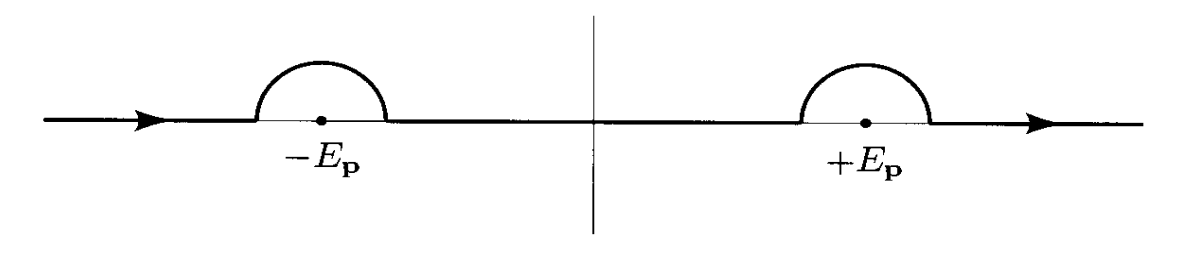
\includegraphics[height=3cm ,width=14cm]{QFT/R_Green.png}
\caption{Retarded Green Function}
\end{figure}
\[(\partial^2-m^2) D_R(x-y) = i \delta(x-y)\]
\[D_F(x-y) \equiv \langle 0 | T\phi(x) \phi(y) | 0 \rangle = \int \frac{d^4 p}{(2\pi)^4} \frac{-i}{p^2+m^2-i\epsilon} e^{ip(x-y)}\]
Here, $T$ stands for time ordering, placing all operators evaluated at later times to the left.
\begin{figure}[!h]
\centering
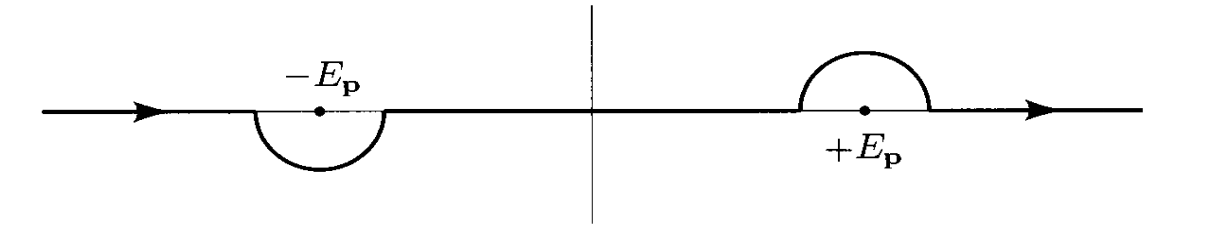
\includegraphics[height=3cm ,width=14cm]{QFT/F_Green.png}
\caption{Feynman Green Function}
\end{figure}

\section{Perturbation theory for canonical quantization}
\[\mathcal{L} = -\frac{1}{2}\partial_{\mu} \phi \partial^{\mu} \phi -\frac{1}{2}m_0^2 \phi^2 -\frac{\lambda_0}{4!}\phi^4\]
\[H = H_0 + H_{int} \quad H_{int} = \int d^3 x \frac{\lambda_0^4}{4!} \phi^4 (\bm{x})\]
\subsection{Perturbation expansion of correlation functions}
\begin{note}
The ground state of the interaction field theory is denoted by $| \Omega \rangle$, the ground state of the free field theory is denoted by $| 0 \rangle$. The zero of energy is defined by $H_0 | 0 \rangle =0$ and $E_0 = \langle \Omega | H | \Omega \rangle$.
\end{note}
\[\phi(t_0,\bm{x}) = \int \frac{d^3p}{(2\pi)^3}( a(\bm{p})e^{i\bm{p}\cdot\bm{x}} + a^{\dagger}(\bm{p})e^{-i\bm{p}\cdot\bm{x}})\]
\[\phi(t,\bm{x}) = e^{iH(t-t_0)} \phi(t_0,\bm{x}) e^{-iH(t-t_0)}\]
\[\phi_I(t,\bm{x}) \equiv e^{iH_0(t-t_0)} \phi(t_0,\bm{x}) e^{-iH_0(t-t_0)}\]
\[H_I(x) = \int d^3x \frac{\lambda_0^4}{4!} \phi_I^4\]
The perturbation expansion of correlation functions is
\[\langle \Omega | T \{ \phi(x) \phi(y) \} | \Omega \rangle = \lim_{T \to \infty(1-i\epsilon)} \frac{\langle 0 | T \left\{ \phi_I(x) \phi_I(y) \mathrm{exp} \left[ -i \int_{-T}^{T} dt H_I \right]\right\} | 0 \rangle}{\langle 0 | T \left\{ \mathrm{exp} \left[ -i \int_{-T}^{T} dt H_I \right]\right\} | 0 \rangle}\]
The proof can be found in chapter 4.2 of \emph{An introduction to quantum field theory (M.E.Peskin \& D.V.Schroeder)}
\begin{newthem}[Wick's theorem]
\[T \left\{ \phi(x_1) \phi(x_2) \cdots \phi(x_n)\right\} = N \left\{ \phi(x_1) \phi(x_2) \cdots \phi(x_n) + \mbox{ all possible contractions }\right\} \]
Normal order : all the $a$'s are to the right of all the $a^{\dagger}$.
\end{newthem}
\noindent
The proof can be found in chapter 4.3 of \emph{An introduction to quantum field theory (M.E.Peskin \& D.V.Schroeder)}
\begin{example}
\begin{eqnarray}
\langle 0 | T \left\{ \phi_I(x_1) \phi_I(x_2) \phi_I(x_3) \phi_I(x_4)\right\}| 0 \rangle &=& D_F(x_1-x_2)D_F(x_3-x_4) \nonumber \\
&+& D_F(x_1-x_3)D_F(x_2-x_4) \nonumber \\
&+& D_F(x_1-x_4)D_F(x_2-x_3) \nonumber
\end{eqnarray}
\end{example}

\subsection{Feynman diagram}
Expand $\langle 0 | T \left\{ \phi_I(x) \phi_I(y) \mathrm{exp} \left[ -i \int_{-T}^{T} dt H_I \right]\right\} | 0 \rangle$ to the first order of $\lambda_0$
\begin{eqnarray}
& &\langle 0 | T \left\{ \phi_I(x) \phi_I(y) \frac{-i\lambda_0}{4!} \int dz^4 \phi_I(z) \phi_I(z) \phi_I(z) \phi_I(z) \right\} | 0 \rangle \nonumber \\
&=& 3 \cdot (\frac{-i\lambda_0}{4!}) D_F(x-y) \int d^4 z D_F(z-z) D_F(z-z) \nonumber \\
&+& 12 \cdot (\frac{-i\lambda_0}{4!}) \int d^4 z  D_F(x-z) D_F(y-z) D_F(z-z) \nonumber
\end{eqnarray}
It can be represented by the so called Feynman diagram.
\begin{figure}[!h]
\centering
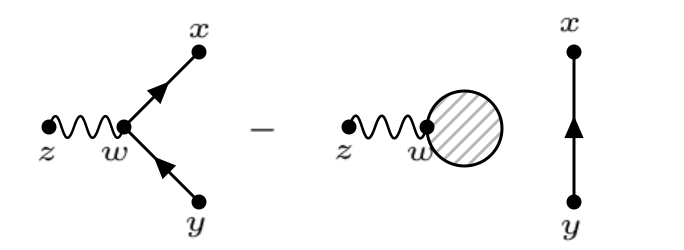
\includegraphics[height=1.5cm ,width=10cm]{QFT/FD1.png}
\caption{Feynman diagram representation of perturbation expansion}
\end{figure}
\\
The symmetry factor of the first diagram is $S = \frac{4!}{3} = 8$.
The symmetry factor of the second diagram is $S = \frac{4!}{12} = 2$.
The Feynman rules for $\phi^4$ theory are:
\begin{enumerate}
\item For each propagator, $P = D_F(x-y)$
\item For each vertex, $V = (-i\lambda_0)\int d^4z$
\item For each external point, $E=1$
\item Divided by the symmetry factor
\end{enumerate}
At last, we can prove that
\[\langle \Omega | T \{ \phi_I(x_1) \phi_I(x_2) \cdots \phi_I(x_n) \} | \Omega \rangle = \mbox{ sum of all E-connected diagrams with n external points}\]
Here, the "E-disconnected" means disconnected from all external points", being called "vacuum bubbles". They vacuum bubbles in $\langle 0 | T \left\{ \phi_I(x_1) \phi_I(x_2) \cdots \phi_I(x_n) \mathrm{exp} \left[ -i \int_{-T}^{T} dt H_I \right]\right\} | 0 \rangle$ are all cancelled by the $\langle 0 | T \left\{ \mathrm{exp} \left[ -i \int_{-T}^{T} dt H_I \right]\right\} | 0 \rangle$.

\section{Path integral formulation}
\subsection{Basic formulation}
\noindent
Recall the path integrals formulation in quantum mechanics, we have
\[\langle \phi_b(\bm{x}) | e^{-iHT} | \phi_a(\bm{x}) \rangle = \int \mathcal{D}\phi \mathcal{D}\pi  \mathrm{exp} \left[ i\int_0^T d^4x (\pi\dot{\phi} - \frac{1}{2}\pi^2 - \frac{1}{2}(\nabla \phi)^2 -V(\phi))\right]\]
Here, $\langle \phi_b(\bm{x}) |$ is the eigenstate of $\phi_S(\bm{x})=\phi_H(\bm{x},0)$ with eigenvalue $\phi_b(\bm{x})$ at time $t=T$,$| \phi_a(\bm{x}) \rangle$ is the eigenstate of $\phi_S(\bm{x})$ with eigenvalue $\phi_a(\bm{x})$ at time $t=0$.\\
Since the exponential is quadratic in $\pi$, we can complete the square and evaluate the $\mathcal{D}(\pi)$ integral to obtain
\[\langle \phi_b(\bm{x}) | e^{-iHT} | \phi_a(\bm{x}) \rangle = \int \mathcal{D}\phi  \mathrm{exp} \left[ i\int_0^T d^4x \mathcal{L} \right]\]
Now we can abandon the Hamiltonian formalism and take the the equation above to define the Hamiltonian dynamics.
\begin{note}
We emphasize that in this subsection, $\phi_H$ denotes the Heisenberg picture of field whose value is operators,$\phi_S$ denotes the Schr\"{o}dinger picture of field, $\phi(x)$ is classical field whose value is ordinary number.
\end{note}

\subsubsection{Correlation function}
\[\langle \Omega | T \phi_H(x_1) \phi_H(x_2)| \Omega \rangle = \lim_{T \to \infty(1-i\epsilon)} \frac{\int \mathcal{D}\phi \phi(x_1)\phi(x_2) \mathrm{exp} \left[ i\int_T^T d^4x \mathcal{L} \right]}{\int \mathcal{D} \phi \mathrm{exp} \left[ i\int_T^T d^4x \mathcal{L} \right]}\]
The proof can be found in chapter 9.2 of \emph{An introduction to quantum field theory (M.E.Peskin \& D.V.Schroeder)}.

\subsubsection{Functional derivatives and the generating functional}
\noindent
We define the generating functional as
\[Z[J] \equiv \int \mathcal{D} \phi \mathrm{exp} \left[ i\int d^4x \mathcal{L} + J(x)\phi(x) \right]\]
We can prove that
\[\langle \Omega | T \phi_H(x_1) \cdots \phi_H(x_n) | \Omega \rangle = \frac{1}{Z_0} \left( -i\frac{\delta}{\delta J(x_1)} \right)\cdots \left( -i\frac{\delta}{\delta J(x_n)} \right) Z[J]|_{J=0}\]
Here, $Z_0 \equiv Z[J=0]$.

\subsection{Free field theory}
\noindent
In Klein-Gordon field theory,
\[\int d^4x [\mathcal{L}_0(\phi)+J\phi] = \int d^4x [\frac{1}{2}\phi (\partial^2 -m^2+i\epsilon)\phi + J\phi]\]
Define
\[\phi'(x) \equiv \phi(x) + \int d^4y (-iD_F(x-y)) J(y) \]
Recall that $(\partial^2-m^2)D_F(x-y) = i\delta(x-y)$, we can derive that
\[\int d^4x [\mathcal{L}_0+J\phi] = \int d^4x [\frac{1}{2}\phi' (\partial^2 -m^2+i\epsilon)\phi'] - \int d^4x d^4y \frac{1}{2} J(x)[-iD_F(x-y)]J(y)\]
After integration, we can know that
\[Z[J] = Z_0 \mathrm{exp} [-\frac{1}{2} \int d^4x d^4y J(x)D_F(x-y)J(y)]\]
So,
\[\langle 0 | T \phi_H(x_1) \phi_H(x_2) | 0 \rangle =  - \frac{\delta}{\delta J(x_1)} \frac{\delta}{\delta J(x_2)} \mathrm{exp} [-\frac{1}{2} \int d^4x d^4y J(x)D_F(x-y)J(y)]|_{J=0} = D_F(x_1-x_2)\]

\section{Perturbation theory for path integral quantization}
\begin{eqnarray}
\mathcal{L} &=& -\frac{1}{2}\partial_{\mu} \phi \partial^{\mu} \phi -\frac{1}{2}m_0^2 \phi^2 -\frac{\lambda_0}{4!}\phi^4 \nonumber \\
\mathcal{L} &=& \mathcal{L}_0 + \mathcal{L}_1 \quad \mathcal{L}_1 =- \frac{\lambda_0}{4!} \phi^4 (\bm{x}) \nonumber \\
Z[J] &=& \int \mathcal{D}\phi e^{i\int d^4x [\mathcal{L}_0 + \mathcal{L}_1 + J\phi]} \nonumber \\
&=& e^{i\int d^4y \mathcal{L}_1(\frac{1}{i} \frac{\delta}{\delta J(y)})} \int \mathcal{D}\phi e^{i\int d^4x [\mathcal{L}_0 + J\phi]} \nonumber \\
&\propto & e^{i\int d^4x \mathcal{L}_1(\frac{1}{i} \frac{\delta}{\delta J(x)})} \mathrm{exp} [-\frac{1}{2} \int d^4y d^4z J(y)D_F(y-z)J(z)] \nonumber \\
& =& \sum_{V=0}^{\infty} \frac{1}{V!} [ \frac{-i\lambda_0}{4!} \int d^4x (\frac{1}{i} \frac{\delta}{\delta J(x)})^4]^V \times \sum_{P=0}^{\infty} \frac{1}{P!} [-\frac{1}{2} \int d^4y d^4z J(y)D_F(y-z)J(z)]^P \nonumber
\end{eqnarray}
If we focus on a term with particular values of V and P, then
the number of surviving sources (after we take all the functional derivatives) is $E = 2P-4V$. The $4V$ functional derivatives can act on the 2P sources in $\frac{(2P)!}{(2P-4V)!}$ different combinations. However, many of the resulting expressions are algebraically identical.\\ \\
To organize them, we introduce Feynman diagrams similar to that in perturbation theory of canonical quantization. In these diagrams, a line segment stands for a propagator $D_F(x-y)$, a filled circle at one end of a line segment for a source $i\int d^4x J(x)$, and a vertex joining four line segments for $-i\lambda_0 \int d^4 z$.\\ \\
For each diagram, we can assign a symmetry factor $S_P$ similar to that in perturbation theory for canonical quantization. Due to the fact that some external sources are identical here, usually $S_P \neq S_C$. But when calculating the correlation function, the exchange of the order of functional derivatives to identical sources can eliminate the difference.\\ \\
We can demonstrate that
\[Z[J] \propto \mathrm{exp}(\sum_I C_I)\]
Here, $C_I$ stands for a particular connected diagram, including its symmetry factor. We define $W[J]$ as
\[Z[J] \equiv Z_0 \mathrm{exp}(-iW[J])\]
As, $W[0]=0$, we know
\[-iW[J] = \sum_{I \neq \{0\}} C_I\]
The notation $I\neq \{0\}$ means that the vacuum diagrams are omitted from the sum.\\
The detailed discussion can be found in chapter 9 of \emph{Quantum field theory (M. Srednicki)}.

\section{LSZ reduction formula}
\subsection{Field strength renormalization}
\noindent
The completeness relation:
\[\bm{1} = |\Omega\rangle\langle\Omega| +  \sum_{\lambda} \int \frac{d^3p}{(2\pi)^3} \frac{1}{2E_{\bm{p}}} |\lambda_{\bm{p}}\rangle\langle\lambda_{\bm{p}}|\]
Here, $E_{\bm{p}} = \sqrt{m_{\lambda}^2 + \bm{p}^2}$\\
\begin{figure}[!h]
\centering
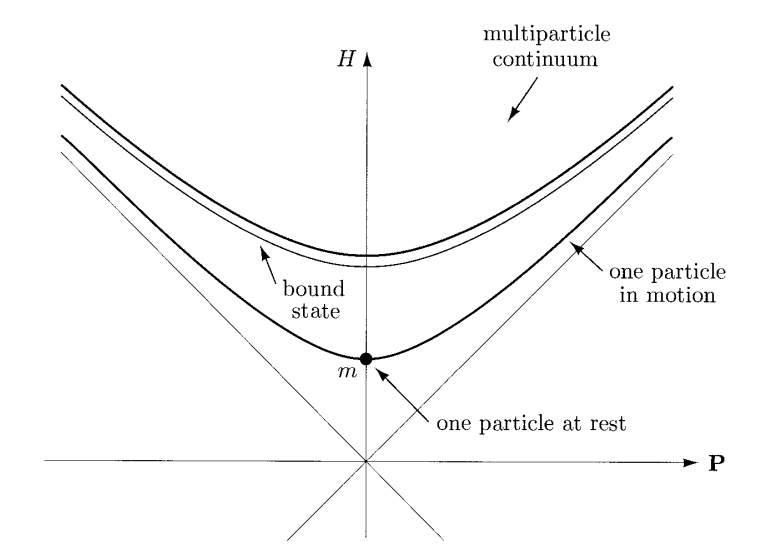
\includegraphics[height=7cm ,width=12cm]{QFT/FSR1.png}
\caption{Particle's energy-momentum relation}
\end{figure}
\\
Assume for now $x^0 > y^0$ and define $\langle \Omega | \phi(x) \phi(y) | \Omega \rangle_{C} = \langle \Omega | \phi(x) \phi(y) | \Omega \rangle - \langle \Omega | \phi(x)| \Omega \rangle \langle | \Omega \phi(y) | \Omega \rangle$ as connected two point function. (The term $\langle \Omega | \phi(x)| \Omega \rangle \langle | \Omega \phi(y) | \Omega \rangle$ is usually zero by symmetry; for higher spin fields, it is zero by Lorentz invariance.) The connected two point function is
\[\langle \Omega | \phi(x) \phi(y) | \Omega \rangle_{C} = \sum_{\lambda} \int \frac{d^3p}{(2\pi)^3} \frac{1}{2E_{\bm{p}}} \langle \Omega | \phi(x) |\lambda_{\bm{p}}\rangle\langle\lambda_{\bm{p}}| \phi(y) | \Omega \rangle\]
It can be verified that
\[\langle \Omega | \phi(x) |\lambda_{\bm{p}}\rangle = \langle \langle \Omega | \phi(0) | \lambda_0 \rangle e^{ipx} |_{p^0 = E_{\bm{p}}}\]
So,
\[\langle \Omega | \phi(x) \phi(y) | \Omega \rangle_C = \sum_{\lambda} \int \frac{d^4p}{(2\pi)^4} \frac{-i}{p^2 + m_{\lambda}^2 -i\epsilon} e^{ip(x-y)} |\langle \Omega | \phi(0) | \lambda_0 \rangle|^2\]
Analogous expressions hold for the case $y^0 > x^0$, and both cases can be summarized as
\[\langle \Omega | T \phi(x) \phi(y) | \Omega \rangle_C = \int_0^{\infty} \frac{dM^2}{2\pi} \rho(M^2) D_F(x-y;M^2)\]
and 
\[\rho(M^2) = \sum_{\lambda} (2\pi) \delta(M^2-m^2)|\langle \Omega | \phi(0) | \lambda_0 \rangle|^2 \]
\begin{figure}[!h]
\centering
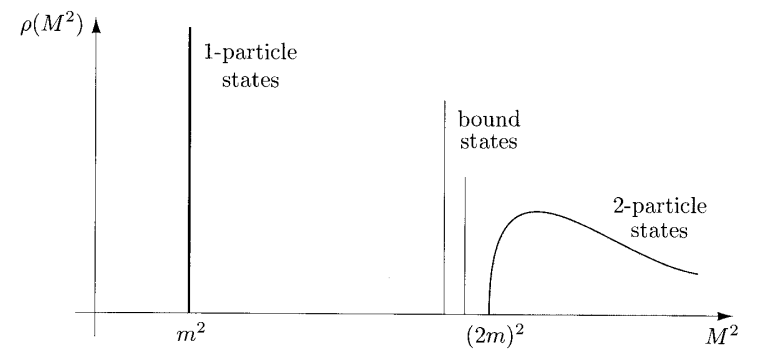
\includegraphics[height=5cm ,width=12cm]{QFT/FSR2.png}
\caption{The structure of the spectral density function $\rho(M^2)$}
\end{figure}\\
The one-particle state contribute an isolated delta function to the spectral density function, so
\[\rho(M^2) = 2\pi \delta (M^2 -m^2) \cdot Z + \mbox{ (nothing else until $M^2 > \sim (2m)^2$) }\]
$Z = |\langle \Omega | \phi(0) | \lambda_0 \rangle|^2$ is called field-strength renormalization. $m$ is the physical mass of a single particle of the $\phi$ boson. The Fourier transformation of the two point function is
\begin{eqnarray}
&\phantom{=}& \int d^4x e^{-ipx} \langle \Omega | T \phi(x) \phi(0) | \Omega \rangle_C \nonumber \\  
&=& \int_{0}^{\infty} \frac{dM^2}{2\pi} \rho(M^2) \frac{-i}{p^2+M^2-i\epsilon} = \frac{-iZ}{p^2+m^2-i\epsilon} +  \int_{\sim 4m^2}^{\infty} \frac{dM^2}{2\pi} \rho(M^2) \frac{-i}{p^2+M^2-i\epsilon} \nonumber
\end{eqnarray}
\begin{figure}[!h]
\centering
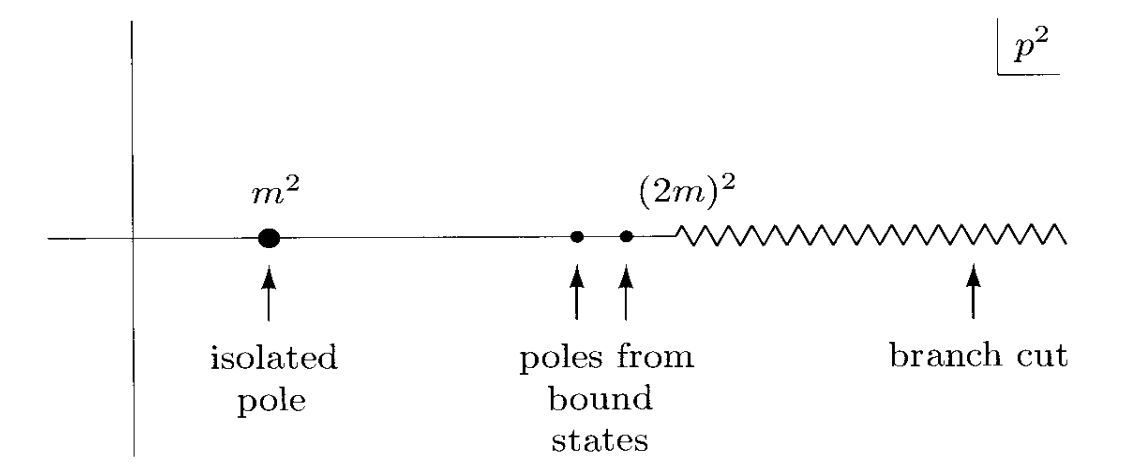
\includegraphics[height=4cm ,width=12cm]{QFT/FSR3.png}
\caption{The structure of the two point function in Fourier space}
\end{figure}
\vspace{80pt}
\subsection{LSZ reduction formula}
\begin{newthem}[LSZ reduction formula]
\begin{eqnarray}
&& \quad \prod_1^n \int d^4 x_i e^{-ip_ix_i} \prod_1^m d^4 y_j e^{ik_jy_j} \langle \Omega | T \{\phi(x_1) \cdots \phi(x_n) \phi(y_1) \cdots \phi(y_m)\} | \Omega \rangle \nonumber \\
&& \underset{ p_i^0 \to E_{\bm{p}_i}\, k_i^0 \to E_{\bm{k}_i}}{\sim}  \left( \prod_1^n \frac{-\sqrt{Z} i}{p_i^2 + m^2 -i\epsilon} \right) \left( \prod_1^m \frac{-\sqrt{Z} i}{k_i^2 + m^2 -i\epsilon} \right) \langle \bm{p}_1 \cdots \bm{p}_n | S | \bm{k}_1 \cdots \bm{k}_m \rangle \nonumber
\end{eqnarray}
\end{newthem}
\noindent
The $\sim$ means the two sides of the expression share the same singular structure around $p_i^0 \to E_{\bm{p}_i}$, $k_i^0 \to E_{\bm{k}_i}$.
The proof can be found in chapter 7.2 of \emph{An introduction to quantum field theory (M.E.Peskin \& D.V.Schroeder)}.
To express the formula above in the language of Feynman diagrams, we consider the S-matrix element for 2-particle $\to$ 2-particle for example. Note the disconnected diagram should be disregarded because they do not have the singularity structure with a product of four poles indicated by on the right side of the LSZ reduction formula. So, the exact four point function
\[\prod_1^2 \int d^4 x_i e^{-ip_ix_i} \prod_1^2 d^4 y_i e^{ik_jy_j} \langle \omega | T \{\phi(x_1)\phi(x_2)\phi(y_1) \phi(y_2)\} | \Omega \rangle \]
has the general form showed as below.
\begin{figure}[!h]
\centering
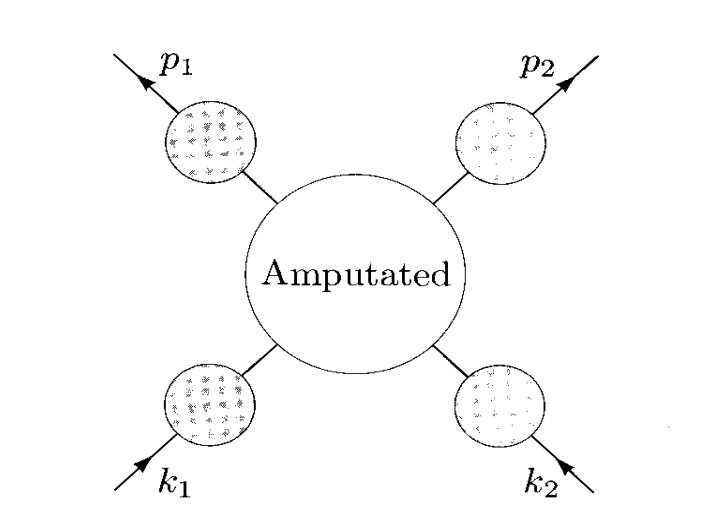
\includegraphics[height=3cm ,width=3.75cm]{QFT/LSZ1.png}
\caption{Amputated Feynman diagram}
\end{figure}\\
\begin{note}
One-particle-irreducible, or 1PI for short, refers to diagrams that is still connected after one line is cut
\end{note}
\noindent
We can sum up the corrections to each external leg. Let $-iM^2(p^2)$ denote the sum of all 1PI insertions into the scalar propagator:
\begin{figure}[!h]
\centering
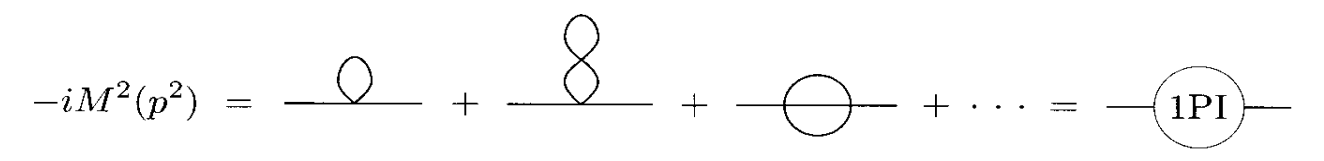
\includegraphics[height=2cm ,width=15cm]{QFT/LSZ2.png}
\caption{Diagram representation of 1PI propagator}
\end{figure}\\
Then the exact propagator can be written as a geometric series in
Figure 2.9.
\begin{figure}[!h]
\centering
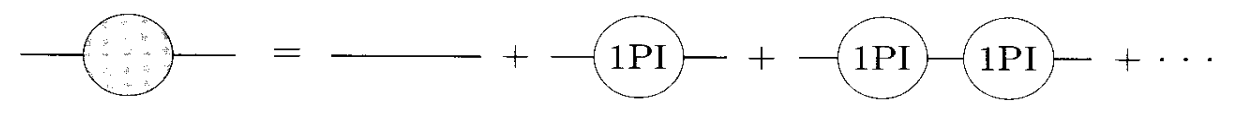
\includegraphics[height=1.5cm ,width=15cm]{QFT/LSZ3.png}
\caption{Diagram representation of exact propagator}
\end{figure}\\
The result is $\frac{-i}{p^2 + m_0^2 + M^2}$. If we expand each resummed propagator about the physical particle pole, we see that each external leg of the four-point amplitude contributes
\[\frac{-i}{p^2 + m_0^2 + M^2} \underset{p^0 \to E_{\bm{p}}}{\sim} \frac{-iZ}{p^2+m^2} + \mbox{ (regular) }\]
Thus, the sum of diagrams contains a product of four point poles:
\[\frac{-iZ}{p_1^2 + m^2} \frac{-iZ}{p_2^2 + m^2} \frac{-iZ}{k_1^2 + m^2} \frac{-iZ}{k_2^2 + m^2}\]
So, the S matrix element can be represented by 
\begin{figure}[!h]
\centering
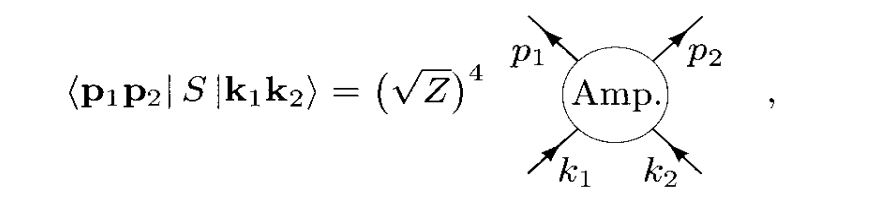
\includegraphics[height=3cm ,width=12cm]{QFT/LSZ4.png}
\caption{Feynman diagram representation of LSZ reduction formula}
\end{figure}\\
It is easy to be generalized to the more complicated scattering cases. After Fourier transforming the n-point function to momentum space and cutting off the external legs, the Feynman rules for S-matrix element can be stated as follows:
\begin{enumerate}
\item For each propagator, $P = \frac{-i}{p^2 + m_0^2 -i\epsilon}$;
\item For each vertex, $V = -i\lambda_0$;
\item For each external point, $E=1$;
\item Impose momentum conservation at each vertex;
\item Integrate over each undetermined loop momentum: $\int \frac{d^4p}{(2\pi)^4}$;
\item Divided by the symmetry factor;
\item Multiply the total momentum conservation factor $(2\pi)^4 \delta(\sum p_f - \sum p_i)$ 
\end{enumerate}
We can write $\langle f | S | i \rangle = i \mathcal{M} (2\pi)^4 \delta(\sum p_f - \sum p_i)$ for convenience.

\section{Renormalization}
\noindent
Renormalization, the procedure in quantum field theory by which divergent parts of a calculation, leading to nonsensical infinite results, are absorbed by redefinition into a few measurable quantities, so yielding finite answers.

\subsection{Counting of ultraviolet divergence}
\noindent
Consider a pure scalar theory in $d$ dimensions with a $\phi^n$ interaction term
\[\mathcal{L} = -\frac{1}{2} \partial^{\mu} \phi \partial_{\mu} \phi -\frac{1}{2}m^2 \phi^2 - \frac{\lambda}{n!}\phi^n\]
Let $N$ be the number of external lines in the diagram, $P$ the number of propagators, $V$ the number of vertices. The number of the loops in the diagram is $L=P-V+1$.  There are $n$ lines meeting at each vertex, so $nV = 2P+N$. Loosely speaking, each loop has an integral $d^d p$, each propagator has a factor $p^{-2}$, so the superficial degrees of divergence is
\[D = dL - 2P = d + [n(\frac{d-2}{2})-d)]V - (\frac{d-2}{2})N\]
According the superficial degrees of divergence of the diagram. These three possible types of ultraviolet behaviour of quantum field theories. We will refer to them as follows

\begin{enumerate}
\item Super-renormalizable theory: Only a finite number of Feynman diagrams superficially diverge.
\item renormalizable theory: Only a finite number of amplitudes superficially diverge; however, divergences
occur at all orders in perturbation theory. 
\item Non-renormalizable theory: All amplitudes are divergent at a sufficiently high order in perturbation
theory.
\end{enumerate}

So, for $\phi^4$ theory in four dimension, $D = 4 - N$. It is a renormalizable theory. For $\phi^3$ theory in four dimension, $D = 4 - V -N$. It is a super-renormalizable theory. For $\phi^6$ theory in four dimension, $D = 4 + 2V -N$. It is a Non-renormalizable theory. \\ \\
The superficial degrees of freedom can also be derived from dimensional analysis. The dimension of $\lambda$ is $d - \frac{n(d-2)}{2}$. Now consider an arbitrary diagram with $N$ external lines. One way that such a diagram could arise is from an interaction term $\eta \phi^N$ in the Lagrangian. The dimension of $\eta$ would then be $d - \frac{N(d-2)}{2}$, and therefore we conclude that any (amputated) diagram with $N$ external lines has dimension $d - \frac{N(d-2)}{2}$. In our theory with only the $\lambda \phi^n$ vertex, if the diagram has $V$ vertices, its divergent part is proportional to $\lambda^V \Lambda^D$, where $\Lambda$ is a high momentum cut-off and $D$ is the superficial degree of divergence.  Applying dimensional analysis, we find
\[d - \frac{N(d-2)}{2} = V[d - \frac{n(d-2)}{2}] + D\]
Note that the quantity that multiplies $V$ in this expression is just the dimension of the coupling constant $\lambda$. Thus we can characterize the three degrees of renormalizability in a second way:

\begin{enumerate}
\item Super-renormalizable: Coupling constant has positive mass dimension.
\item  renormalizable: Coupling constant is dimensionless.
\item  Non-renormalizable: Coupling constant has negative mass dimension.
\end{enumerate}

\subsection{Renormalized perturbation theory}
The Lagrangian of $\phi^4$ theory is 
\[\mathcal{L} = -\frac{1}{2} \partial^{\mu} \phi \partial_{\mu} \phi -\frac{1}{2}m_0^2 \phi^2 - \frac{\lambda_0}{4!}\phi^4\]

We write $m_0$ and $\lambda_0$, to emphasize that these are the bare values of the mass and coupling constant, not the values measured in experiments.
Since the theory is invariant under $\phi \to -\phi$, all amplitudes with an odd number of external legs vanish. The only divergent amplitudes are therefore
\begin{figure}[!h]
\centering
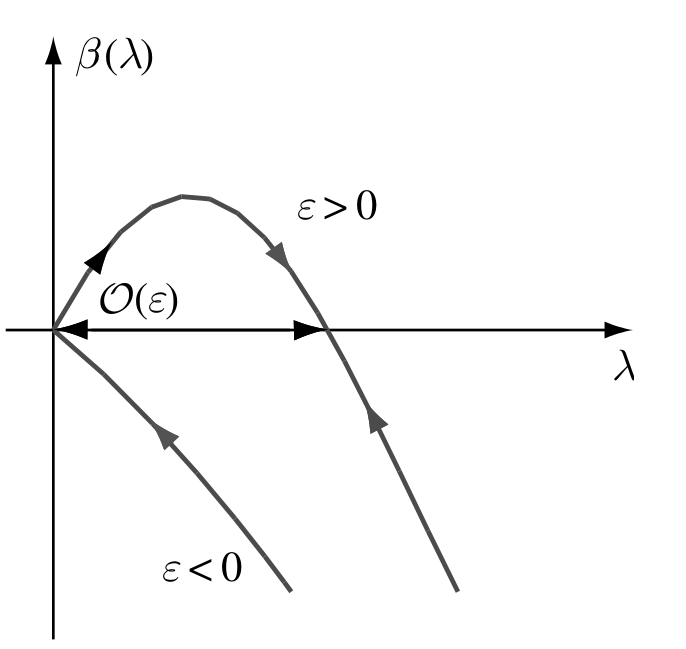
\includegraphics[height=4cm ,width=9cm]{QFT/RG1.png}
\caption{Divergence of $\phi^4$ theory}
\end{figure}

Ignoring the vacuum diagram, these amplitudes contain three infinite constants. Our goal is to absorb these constants into the three unobservable parameters of the theory: the bare mass, the bare coupling constant, and the field strength. To accomplish this goal, it is convenient to reformulate the perturbation expansion so that these unobservable quantities do not appear
explicitly in the Feynman rules. Recall that the exact two-point function has the form
\[\int d^4x \langle \Omega | \phi(x) \phi(0) | \Omega \rangle e^{-ipx} = \frac{-iZ}{p^2+m^2} + \mbox{ terms regular at } p^2 = m^2\]
We can eliminate the $Z$ from this equation by rescaling the field:
$\phi = Z^{\frac{1}{2}} \phi_r$
We also define
\[\delta_Z = Z -1 \quad \delta_m = Zm_0^2 - m^2 \quad \delta_{\lambda} = \lambda_0 Z^2 - \lambda\]
Then the Lagrangian becomes
\[\mathcal{L} = -\frac{1}{2} \partial^{\mu} \phi_r \partial_{\mu} \phi_r -\frac{1}{2}m^2 \phi_r^2 - \frac{\lambda}{4!}\phi_r^4 -\frac{1}{2} \delta_Z \partial^{\mu} \phi_r \partial_{\mu} \phi_r -\frac{1}{2}\delta_m \phi_r^2 - \frac{\delta \lambda}{4!}\phi_r^4\]
The last three terms, known as counter-terms, have absorbed the infinite but unobservable shifts between the bare parameters and the physical parameters.We give precise definitions of the physical mass and coupling constant as Figure 2.12.\\
\begin{figure}[!h]
\centering
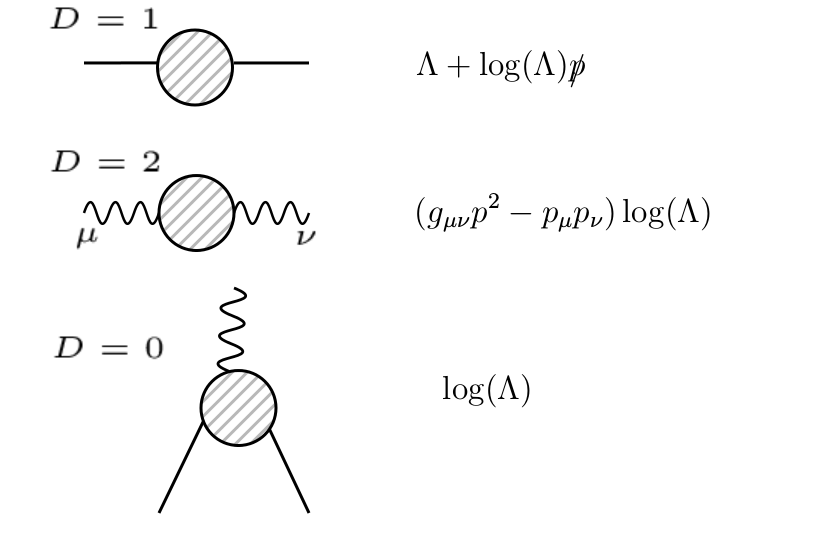
\includegraphics[height=3cm ,width=11cm]{QFT/RG2.png}
\caption{Renormalization condition}
\end{figure}

The renormalization scheme here is called on-shell (OS) scheme. Other renormalization scheme would be introduced later.
These equations are called renormalization conditions.
Our new Lagrangian gives a new set of Feynman rules as Figure 2.13.
\begin{figure}[!h]
\centering
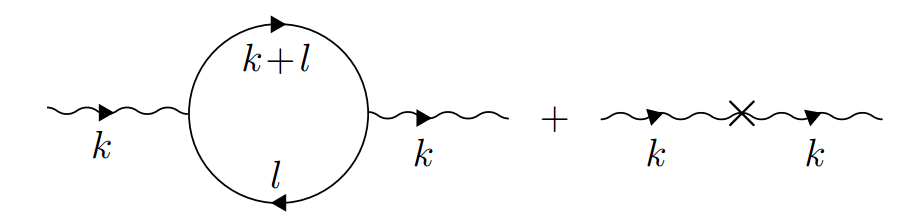
\includegraphics[height=6cm ,width=9cm]{QFT/RG3.png}
\caption{Feynman rules for renormalized perturbation theory}
\end{figure}

We can use these new Feynman rules to compute any amplitude in $\phi^4$ theory. The procedure is as follows. Compute the desired amplitude as the sum of all possible diagrams created from the propagator and vertices shown above. The loop integrals in the diagrams will often diverge, so one must introduce a regulator. The result of this computation will be a function of the three unknown parameters $\delta_Z$, $\delta_m$, and $\delta_{\lambda}$. Adjust ( or "renormalise") these three parameters as necessary to maintain the renormalization conditions. After this adjustment, the expression for the amplitude should be finite and independent of the regulator.

This procedure, using Feynman rules with counter-terms, is known as renormalized perturbation theory. 

\subsubsection{Mandelstam variable}
In theoretical physics, the \href{https://en.wikipedia.org/wiki/Mandelstam_variables}{\textbf{Mandelstam variable}}  are numerical quantities that encode the energy, momentum, and angles of particles in a scattering process in a Lorentz-invariant fashion. They are used for scattering processes of two particles to two particles. 
The Mandelstam variables $s$, $t$, $u$ are then defined by
\begin{eqnarray}
s=-(p_{1}+p_{2})^{2}=-(p_{3}+p_{4})^{2} \nonumber \\
t=-(p_{1}-p_{3})^{2}=-(p_{2}-p_{4})^{2} \nonumber \\
u=-(p_{1}-p_{4})^{2}=-(p_{2}-p_{3})^{2} \nonumber
\end{eqnarray}

Where $p_1$ and $p_2$ are the four-momenta of the incoming particles and $p_3$ and $p_4$ are the four-momenta of the outgoing particles.
$s$ is also known as the square of the center-of-mass energy (invariant mass) and $t$ is also known as the square of the four-momentum transfer.\\
We can verify that
\[s+t+u = m_1^2 + m_3^2 + m_3^2 +m_4^2\]

\subsection{Techniques for renormalization}
\subsubsection{Feynman's formula}
\begin{newthem}[Feynman's formula]
\[ \frac{1}{A_1 \cdots A_n} = \int dF_n (x_1A_1+ \cdots +x_nA_n)^{-n}\]
where the integration measure over the Feynman parameters $x_i$ is
\[\int dF_n = (n-1)! \int_0^1 dx_1 \cdots dx_n \delta(x_1+\cdots+x_n-1)\]
This measure is normalized so that
\[\int dF_n = 1\]
A generalization of Feynman's formula is
\[ \frac{1}{A_1^{\alpha_1} \cdots A_n^{\alpha_n}} = \frac{\Gamma(\sum_i \alpha_i)}{\prod_i \Gamma(\alpha_i)} \frac{1}{(n-1)!}\int dF_n \frac{\prod_i x_i^{\alpha_i-1}}{(\sum_i x_i A_i)^{\sum_i \alpha_i}}\]
\end{newthem}
\begin{figure}[!h]
\centering
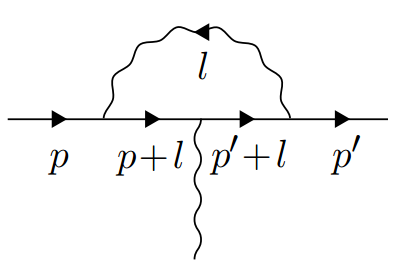
\includegraphics[height=5cm ,width=8cm]{QFT/RG5.png}
\caption{Wick rotation}
\end{figure}

\subsubsection{Wick rotation}
For an integral $\int d^d q f(q^2-i\epsilon)$, if the integrand vanishes fast enough as $|q_0| \to \infty$, we can rotate this contour clockwise by $\frac{\pi}{2}$, so that it runs from $-i\infty$ to $i\infty$. In making this Wick rotation, the contour does not pass over any poles. (The $i\epsilon$ are needed to make this statement unambiguous.) Thus the value of the integral is unchanged. It is now convenient to define a Euclidean d-dimensional vector $\bar{q}$ via $q^0 = i \bar{q}_d$ and $q_j = \bar{q}_j$; then $q^2 = \bar{q}^2$, where
\[\bar{q}^2 = \bar{q}_1^2 + \cdots + \bar{q}_d^2\]
Also, $d^dq = id^d \bar{q}$.Therefore, in general,
\[\int d^d q f(q^2-i\epsilon) = i \int d^d\bar{q} f(\bar{q}^2)\]

\subsubsection{Dimensional regularization}
Dimensional regularization is a method for regularizing integrals in the evaluation of Feynman diagrams. For example, if one wishes to evaluate a loop integral which is logarithmically divergent in four dimensions, like
\[\int {\frac {d^{d}p}{(2\pi )^{d}}}{\frac {1}{\left(p^{2}+m^{2}\right)^{2}}}\]

One first rewrites the integral in some way so that the number of variables integrated over does not depend on d, and then we formally vary the parameter $d$, to include non-integral values like $d=4-\epsilon$.
\[\int _{0}^{\infty }{\frac {dp}{(2\pi )^{4-\varepsilon }}}{\frac {2\pi ^{(4-\varepsilon )/2}}{\Gamma \left({\frac {4-\varepsilon }{2}}\right)}}{\frac {p^{3-\varepsilon }}{\left(p^{2}+m^{2}\right)^{2}}}={\frac {2^{\varepsilon -4}\pi ^{{\frac {\varepsilon }{2}}-1}}{\sin({\frac {\pi \varepsilon }{2}})\Gamma (1-{\frac {\varepsilon }{2}})}}m^{-\varepsilon }={\frac {1}{8\pi ^{2}\varepsilon }}-{\frac {1}{16\pi ^{2}}}\left(\ln {\frac {m^{2}}{4\pi }}+\gamma \right)+{\mathcal {O}}(\varepsilon )\]
There is a useful formula for calculating the integral
\[\int \frac{d^d \bar{q}}{(2\pi)^{d}} \frac{(\bar{q}^2)^a}{(\bar{q}^2+D)^b} = \frac{\Gamma(b-a-\frac{1}{2}d) \Gamma(a+\frac{1}{2}d)}{(4\pi)^{d/2} \Gamma(b) \Gamma(\frac{1}{2}d)} D^{-(b-a-d/2)}\]
If $a=0$, then the formula will be
\[\int \frac{d^d \bar{q}}{(2\pi)^{d}} \frac{1}{(\bar{q}^2+D)^b} = \frac{\Gamma(b-\frac{1}{2}d)}{(4\pi)^{d/2} \Gamma(b)} D^{-(b-d/2)}\]

\subsection{One loop structure of $\phi^4$ theory}
First consider the basic two-particle scattering amplitude,
\begin{figure}[!h]
\centering
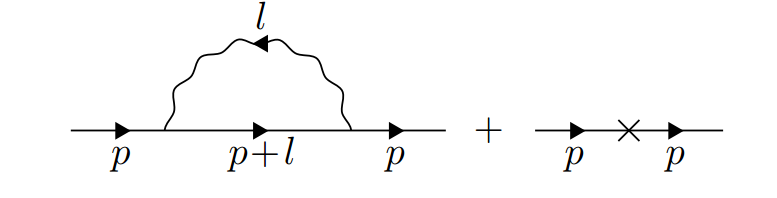
\includegraphics[height=3cm ,width=11cm]{QFT/RG4.png}
\caption{Feynman diagram representation of two-particle scattering to one loop}
\end{figure}
If we define $p = p_1 + p_2$, then the second diagram of Figure 2.15 is
\[\frac{(-i\lambda)^2}{2} \int \frac{d^4k}{(2\pi)^4} \frac{-i}{k^2+m^2} \frac{-i}{(k+m)^2+m^2} \equiv (-i\lambda)^2 iV(-p^2)\]
So the entire amplitude is therefore
\[i\mathcal{M} = -i\lambda + (-i\lambda)^2 [iV(s) + iV(t) iV(u)] -i\delta_{\lambda} + \mathcal{O}(\lambda^3)\]
To keep $\lambda$ dimensionless in dimensional regularization, we can make the transformation $\lambda \to \lambda \tilde{\mu}^{\epsilon}$. Here, $\mu$ is an arbitrary number with mass dimension 1 and $\epsilon \equiv 4-d$. 

We can calculate that
\[V(-p^2) = -\frac{1}{32\pi^2} \int_0^1 (\frac{2}{\epsilon} + \ln(\frac{\mu^2}{D(-p^2)}))\]
where $\mu \equiv  \sqrt{4\pi} e^{-\gamma/2} \tilde{\mu}$, $D(-p^2) = x(1-x)p^2+m^2$

The renormalization condition implies that
\[\delta_{\lambda} = -\lambda^2[V(4m^2)+2V(0)] + \mathcal{O}(\lambda^3)\]
So,
\[i\mathcal{M} = -i\lambda -\frac{i\lambda^2}{32\pi^2} \int_0^1 dx \left[\ln(\frac{D(s)}{D(4m^2)}) +\ln(\frac{D(t)}{D(0)})+\ln(\frac{D(u)}{D(0)})\right] + \mathcal{O}(\lambda^3)\]
To determine $\delta_Z$ and $\delta_m$ we must compute the two-point function. Define $-iM(p^2)$ as the sum of all one-particle-irreducible insertions into the propagator.The full two-point function is given by
\[\frac{-i}{p^2 + m^2 + M^2}\]
The renormalization conditions require that the pole in this full propagator occur at $p^2=-m^2$ and have residue $1$. These two conditions are equivalent, respectively, to
\[M^2(p^2)|_{p^2=-m^2} = 0 \quad \frac{d}{dp^2} M^2(p^2)|_{p^2=-m^2} =0\]
We can calculate that
\[-iM^2(p^2) = \frac{i\lambda}{32\pi^2}(\frac{2}{\epsilon} + \ln(\frac{\mu^2}{m^2})+1)m^2 -i(p^2\delta_Z + \delta_m)\]
So, to the order of $\lambda$, 
\[\delta_Z=\mathcal{O}(\lambda^2) \quad \delta_m = \frac{\lambda}{32\pi^2}(\frac{2}{\epsilon} + \ln(\frac{\mu^2}{m^2})+1)m^2 + \mathcal{O}(\lambda^2) \quad M^2(p^2) =\mathcal{O}(\lambda^2)\]

The detailed calculation can be found in chapter 10.2 of \emph{An introduction to quantum field theory (M.E.Peskin \& D.V.Schroeder)} and will be eliminated here.

\subsubsection{Perturbation theory to all orders}
We begin by summing all one-particle irreducible diagrams with two
external lines; this gives us the self-energy. We next sum all 1PI
diagrams with four external lines; this gives us the four-point vertex function $V_4(k_1, k_2, k_3, k_4)$. Order by order in $\lambda$, we must adjust the value of the lagrangian coefficients $\delta_Z$, $\delta_m$, and $\delta_{\lambda}$ to maintain the conditions $M^2(-m^2) = 0$, $\frac{dM^2}{dp^2}(-m^2) = 0$, and $V_4(s=4m^2) =0$. 

Next we will construct the n-point vertex functions $V_n$ with $4 < n \leq E$, where $E$ is the number of external lines in the process of interest. We compute these using a skeleton expansion. This means that we draw all the contributing 1PI diagrams, but omit diagrams that include either propagator or three-point vertex corrections. That is, we include only diagrams that are not only 1PI, but also 2PI and 3PI: they remain connected when any one, two, or three lines are cut. (Cutting three lines may isolate a single treelevel vertex, but nothing more complicated.) Then we take the propagators and vertices in these diagrams to be given by the exact propagator $\frac{-i}{p^2+m^2+M^2(p^2)}$ and vertex $V_4(k_1,k_2,k_3,k_4)$, rather than by the tree-level propagator and vertex. We then sum these skeleton diagrams to get $V_n$ for $4 < n \leq E$. Order by order in $\lambda$, this procedure is
equivalent to computing $V_n$ by summing the usual set of contributing 1PI diagrams.

Next we draw all tree-level diagrams that contribute to the process of interest (which has $E$ external lines), including not only four-point vertices, but also n-point vertices. Then we evaluate these diagrams using the exact propagator for internal lines, and the exact 1PI vertices $V_n$; external lines are assigned a factor of one. We sum these tree diagrams to get the scattering amplitude. Order by order in $\lambda$, this procedure is equivalent to computing the scattering amplitude by summing the usual set of contributing diagrams.

Thus we now know how to compute an arbitrary scattering amplitude
to arbitrarily high order. The procedure is the same in any quantum field theory; only the form of the propagators and vertices change, depending on the spins of the fields.


\subsection{Modified minimal-subtraction scheme}
The Lagrangian of $\phi^4$ theory is
\[\mathcal{L} = -\frac{1}{2} \partial^{\mu} \phi \partial_{\mu} \phi -\frac{1}{2}m^2 \phi^2 - \frac{\lambda}{4!}\phi^4 -\frac{1}{2} \delta_Z \partial^{\mu} \phi \partial_{\mu} \phi -\frac{1}{2}\delta_m \phi_r - \frac{\delta \lambda}{4!}\phi^4\]

For minimal-subtraction scheme, we do not demand that $m$ be the physics mass of the field and $\phi$  create a normalized one-particle state. The physical meaning of $\lambda$ is not expressed directly as well. Instead we choose $\delta_Z$, $\delta_m$ and $\delta_{\lambda}$ to cancel the infinities, and nothing more;
we say that $\delta_Z$, $\delta_m$ and $\delta_{\lambda}$ have no finite parts. It is called the modified minimal-subtraction or $\mathrm{\overline{MS}}$ scheme. ("modified" because we introduced $\mu$ via  $\lambda \to \lambda \tilde{\mu}^{\epsilon}$, with $\mu \equiv  \sqrt{4\pi} e^{-\gamma/2} \tilde{\mu}$; had we set $\mu = \tilde{\mu}$ instead, the scheme would be just plain minimal subtraction or MS.)

For loop corrections to propagator,
\[\delta_Z=\mathcal{O}(\lambda^2) \quad \delta_m = \left[ \frac{\lambda}{16\pi^2} + \mathcal{O}(\lambda^2) \right]\frac{1}{\epsilon}m^2 \quad M^2(p^2) = \frac{\lambda}{32\pi^2}( \ln(\frac{m^2}{\mu^2})-1)m^2 + \mathcal{O}(\lambda^2)\]

Firstly, in the $\mathrm{\overline{MS}}$ scheme, the propagator will no longer have a pole at $k^2=-m^2$. The pole will be somewhere else. However, by definition, the actual physical mass $m_{ph}$ of the particle is determined by the location of this pole: $k^2 = -m_{ph}^2$. Thus, the Lagrangian parameter $m$ is no longer the same as $m_{ph}$. The relation of $m$ and $m_{ph}$ is 
\[m_{ph}^2 = M^2(-m_{ph}^2) + m^2\]
To the lowest order, 
\[m_{ph}^2 = \left[1+\frac{\lambda}{32\pi^2}( \ln(\frac{m^2}{\mu^2})-1)\right] m^2\]
Because $m_{ph}$ is a independent of $\mu$, according to $\frac{d}{d\mu} m_{ph} = 0$, it can be derived that
\[\frac{dm}{d\ln \mu} = \left[\frac{\lambda}{32\pi^2}+\mathcal{O}(\lambda^2)\right] m\]
Furthermore, the residue of this pole is no longer one. Let us call the residue $R$. So, in the LSZ formula, we get a net factor of $\sqrt{R}$ for each external line when using the $\mathrm{\overline{MS}}$ scheme. And in $\phi^4$ theory,
\[R = 1 + \mathcal{O}(\lambda^2)\]
For loop corrections to vertex,
\[\delta_{\lambda} = \left[\frac{3\lambda^2}{16\pi^2} + \mathcal{O}(\lambda^3)\right]\frac{1}{\epsilon}\]
\[i\mathcal{M} = -i\lambda -\frac{i\lambda^2}{32\pi^2} \int_0^1 dx \left[\ln(\frac{D(s)}{\mu^2}) +\ln(\frac{D(t)}{\mu^2})+\ln(\frac{D(u)}{\mu^2})\right] + \mathcal{O}(\lambda^3)\]

\subsection{The renormalization group}
\noindent
The Lagrangian of $\phi^4$ theory is 
\[\mathcal{L} = -\frac{1}{2} \partial^{\mu} \phi_0 \partial_{\mu} \phi_0 -\frac{1}{2}m_0^2 \phi_0^2 - \frac{\lambda_0}{4!}\phi_0^4\]
It can be written as
\[\mathcal{L} = -\frac{1}{2}Z_{\phi} \partial^{\mu} \phi \partial_{\mu} \phi -\frac{1}{2}Z_{m}m^2 \phi^2 - Z_{\lambda} \mu^{\epsilon}\frac{\lambda}{4!}\phi^4\]
So, 
\[\phi_0 = Z_{\phi}^{1/2}\phi \quad m_0 = Z_{\phi}^{-1/2} Z_{m}^{1/2}m \quad \lambda = Z_{\phi}^{-2} Z_{\lambda} \lambda \tilde{\mu}^{\epsilon}\]
After using dimensional regularization, the infinities coming from loop integrals take the form of inverse powers of $\epsilon$. In the  $\mathrm{\overline{MS}}$ renormalization scheme, we choose the Zs to cancel off these powers of $1/\epsilon$, and nothing more. Therefore the Zs can be written as
\begin{eqnarray}
Z_{\phi} = 1 + \sum_{n=1}^{\infty} \frac{a_n(\lambda)}{\epsilon^n} \nonumber \\
Z_{m} = 1 + \sum_{n=1}^{\infty} \frac{b_n(\lambda)}{\epsilon^n} \nonumber \\
Z_{\lambda} = 1 + \sum_{n=1}^{\infty} \frac{c_n(\lambda)}{\epsilon^n} \nonumber 
\end{eqnarray}
In $\phi^4$ theory, $a_1 = \mathcal{O}(\lambda^2)$, $b_1 = \frac{\lambda}{16\pi^2} +  \mathcal{O}(\lambda^2)$,$c_1 = \frac{3\lambda}{16\pi^2} + \mathcal{O}(\lambda^2)$\\
Remember that bare fields and parameters must be independent of $\mu$.Define
\[G(\lambda,\epsilon) \equiv \ln(Z_{\phi}^{-2} Z_{\lambda}) = \sum_{n=1}^{\infty} \frac{G_n(\lambda)}{\epsilon^n}\]
We can calculate $G_1 = c_1 - 2a_1 = \frac{3\lambda}{16\pi^2} + \mathcal{O}(\lambda^2)$.
As $\ln \lambda_0 = G + \ln \lambda + \epsilon \ln \tilde{\mu} $. From the independence of $\lambda_0$, we can derive
\[\left ( 1 + \frac{\lambda G'_1}{\epsilon} + \cdots \right) \frac{d\lambda}{d\ln \mu} + \epsilon \lambda = 0\]
In a renormalizable theory, we should have
\[\frac{d\lambda}{d\ln\mu} = -\epsilon\lambda + \beta(\lambda)\]
So
\[\beta(\lambda) = \lambda^2 G'_1(\lambda)\]
In $\phi^4$ theory, we have $\beta(\lambda) = \frac{3\lambda^2}{16\pi^2} + \mathcal{O}(\lambda^3)$.Define
\[M(\lambda,\epsilon) \equiv \ln(Z_{m}^{1/2} Z_{\phi}^{-1/2}) = \sum_{n=1}^{\infty} \frac{M_n(\lambda)}{\epsilon^n}\]
We can calculate $M_1 = \frac{1}{2}b_1 - \frac{1}{2}a_1 = \frac{\lambda}{32\pi^2} + \mathcal{O}(\lambda^2)$.
As $\ln m_0 = M + \ln m $, define the anomalous dimension of the mass
\[\gamma_m(\lambda) \equiv \frac{1}{m} \frac{dm}{d \ln \mu}\]
From the independence of $m_0$, we can derive
\[\gamma_m(\lambda) = \lambda M'_1\]
In $\phi^4$ theory, we have $\gamma_m(\lambda) = \frac{\lambda}{32\pi^2} + \mathcal{O}(\lambda^2)$. We can expand $\ln Z_{\phi}$ as
\[\ln Z_{\phi} = \frac{a_1}{\epsilon} + \frac{a_2-\frac{1}{2}a_1^2}{\epsilon^2}\]
Define the anomalous dimension of the field
\[\gamma_{\phi}(\lambda) = \frac{1}{2} \frac{d\ln Z_{\phi}}{d \ln \mu}\]
We can derive
\[\gamma_{\phi}(\lambda) = -\frac{1}{2}\lambda a'_1\]
In $\phi^4$ theory, we have $\gamma_m(\lambda) = \mathcal{O}(\lambda^2)$.
\subsubsection{Callen-Symanzik equation}
\[G^{(n)}(x_1,\cdots,x_n) \equiv \langle \Omega | T \phi(x_1) \cdots \phi(x_n) | \Omega \rangle_C \]
As $G^{(n)}_0 = Z_{\phi}^{n/2} G^{(n)}$, from the independence of bare Green's function, we have
\[\left( \frac{\partial}{\partial \ln \mu} + \beta(\lambda)  \frac{\partial}{\partial \lambda} + \gamma_m(\lambda) m  \frac{\partial}{\partial m} + n \gamma_{\phi}(\lambda)\right)G^{n}(x_1,\cdots,x_n;\lambda,m,\mu) = 0\]

\section{Spontaneous symmetry breaking}
\subsection{Effective action}
\[Z[J] = e^{-iE[J]} = \int \mathcal{D} \phi \exp\left[ i\int d^4x (\mathcal{L}[\phi] + J \phi) \right]\]
Define 
\[\phi_{\mathrm{cl}} (x) \equiv \langle \Omega | \phi(x) | \Omega \rangle_{J}\]
So, we can derive
\[\frac{\delta}{\delta J(x)} E[J] = - \phi_{\mathrm{cl}}(x)\]
Define
\[\Gamma[\phi_{\mathrm{cl}}] \equiv -E[J] - \int d^4y J(y) \phi_{\mathrm{cl}}(y)\]
We can verify that
\[\frac{\delta}{\delta \phi_{\mathrm{cl}}(x)} \Gamma[\phi_{\mathrm{cl}}] = -J(x)\]
If the external source is set to zero, the effective action satisfy the equation
\[\frac{\delta}{\delta \phi_{\mathrm{cl}}(x)} \Gamma[\phi_{\mathrm{cl}}] = 0\]

The solution to this equation are the values of $\langle \phi(x) \rangle$ in the stable quantum states of the theory. For a translational-invariant vacuum state, we will find a solution in which $\phi_{\mathrm{cl}}$ is independent of $x$. 
For the field theory that the possible vacuum states are invariant under translations and Lorentz transformations, for each possible vacuum states, the corresponding solution $\phi_{\mathrm{cl}}$ will be a constant, independent of $x$.
If $T$ is the time extent of the region and $V$ is its three dimensional volume, we can write
\[\Gamma[\phi_{\mathrm{cl}}] = -(VT) \cdot V_{\mathrm{eff}}(\phi_{\mathrm{cl}})\]

The coefficient $V_{\mathrm{eff}}$ is called effective potential. The condition that $\Gamma[\phi_{\mathrm{cl}}]$ has an extreme then reduces to the simple equation
\[\frac{\partial}{\partial \phi_{\mathrm{cl}}} V_{\mathrm{eff}}(\phi_{\mathrm{cl}}) = 0\] 

A system with spontaneously broken symmetry will have several minimum of $V_{\mathrm{eff}}$, all with the same energy by virtue of the symmetry. The choice of one among these vacuum is the spontaneous symmetry breaking.

\subsection{Computation of the effective action}
\noindent
Decompose the Lagrangian into a piece depending on renormalized parameters and one containing the counter-terms
\[\mathcal{L} = \mathcal{L}_1 + \delta \mathcal{L}\]
Define $J_1$ by
\[\frac{\delta \mathcal{L}_1}{\delta \phi} |_{\phi = \phi_{\mathrm{cl}}} + J_1(x) = 0\]
Define $\delta J$ by
\[J(x) = J_1(x) + \delta J(x)\]
So, we have
\[e^{-iE[J]} = \int \mathcal{D}\phi e^{i\int d^4x (\mathcal{L}_1 + J_1\phi)} e^{i\int d^4x (\delta \mathcal{L} + \delta J \phi)}\]
Replace $\phi$ by $\phi_{\mathrm{cl}}+\eta$,
\begin{eqnarray}
\int d^4x \, (\mathcal{L}_1 + J_1\phi) &=& \int d^4x \, (\mathcal{L}_1[\phi_{\mathrm{cl}}] + J_1\phi_{\mathrm{cl}}) + \int d^4x \, \eta(x) \left( \frac{\delta \mathcal{L}_1}{\delta \phi} + J_1 \right) \nonumber \\
&+& \frac{1}{2} \int d^4x \, d^4y \, \eta(x) \eta(y) \frac{\delta^2 \mathcal{L}_1}{\delta \phi(x) \delta \phi(y)} \nonumber \\
&+& \frac{1}{3!} \int d^4x \, d^4y \, d^4z \, \eta(x) \eta(y) \eta(z) \frac{\delta^3 \mathcal{L}_1}{\delta \phi(x) \delta \phi(y) \delta \phi(z)} + \cdots \nonumber
\end{eqnarray}
The term linear in $\eta$ vanishes by definition of $J_1$.  Keeping only the term up to quadratic order in $\eta$ and still neglecting the counter-terms, we have a pure Gaussian integral, which can be evaluated in terms of a functional determinant:
\begin{eqnarray}
&&\int \mathcal{D}\eta \exp \left[ i \left( \int ( \mathcal{L}_1 [\phi_{\mathrm{cl}}] + J_1\phi_{\mathrm{cl}} ) +  \frac{1}{2} \int \eta \frac{\delta^2 \mathcal{L}_1}{\delta \phi \delta \phi} \eta \right) \right] \nonumber \\
&=& \exp \left[ i \int ( \mathcal{L}_1 [\phi_{\mathrm{cl}}] + J_1\phi_{\mathrm{cl}} )\right] \left( \det \left[  \frac{\delta^2 \mathcal{L}_1}{\delta \phi \delta \phi} \right] \right) ^{-\frac{1}{2}} \nonumber
\end{eqnarray}
Finally, put back the effects of the counter-term Lagrangian,writing it as
\[(\delta \mathcal{L}[\phi_{\mathrm{cl}}] + \delta J \phi_{\mathrm{cl}} ) + ( \delta \mathcal{L}[\phi_{\mathrm{cl}} + \eta] - \delta\mathcal{L} [\phi_{\mathrm{cl}}] + \delta J \eta)\]
Define
\[\mathcal{L}_2 = \left(\frac{1}{3!} \int d^4x \, d^4y \, d^4z \, \eta(x) \eta(y) \eta(z) \frac{\delta^3 \mathcal{L}_1}{\delta \phi(x) \delta \phi(y) \delta \phi(z)} + \cdots \right) + ( \delta \mathcal{L}[\phi_{\mathrm{cl}} + \eta] - \delta\mathcal{L} [\phi_{\mathrm{cl}}] + \delta J \eta)\]
So
\[e^{-iE[J]} = \exp \left[ i \int ( \mathcal{L}_1 [\phi_{\mathrm{cl}}] + J_1\phi_{\mathrm{cl}} + \delta \mathcal{L}[\phi_{\mathrm{cl}}] + \delta J \phi_{\mathrm{cl}} )\right] e^{i\int \mathcal{L}_2(\frac{1}{i} \frac{\delta}{\delta I})} \int \mathcal{D}\eta e^{i\int \left(\frac{1}{2} \eta \frac{\delta^2 \mathcal{L}_1}{\delta \phi \delta \phi} \eta + I\eta \right)}\]
Therefore, define propagator as
\[D_F \equiv i \left( \frac{\delta^2 \mathcal{L}_1}{\delta \phi \delta \phi}\right)^{-1}\]
We have
\[e^{-iE[J]} = \exp \left[ i \int ( \mathcal{L}_1 [\phi_{\mathrm{cl}}] + J_1\phi_{\mathrm{cl}} + \delta \mathcal{L}[\phi_{\mathrm{cl}}] + \delta J \phi_{\mathrm{cl}} )\right] \left( \det \left[  \frac{\delta^2 \mathcal{L}_1}{\delta \phi \delta \phi} \right] \right) ^{-\frac{1}{2}} e^{i\int \mathcal{L}_2(\frac{1}{i} \frac{\delta}{\delta I})} \int \mathcal{D}\eta e^{i\int \left(-\frac{1}{2} I D_F I \right)} |_{I=0}\]
Similar to the procedure in the perturbation theory for path integral quantization, we can get a perturbation expansion for $iE[J]$ using connected Feynman diagram,
\[-iE[J] = i \int ( \mathcal{L}_1 [\phi_{\mathrm{cl}}] + J_1\phi_{\mathrm{cl}} + \delta \mathcal{L}[\phi_{\mathrm{cl}}] + \delta J \phi_{\mathrm{cl}} ) - \frac{1}{2} \log \det \left[  \frac{\delta^2 \mathcal{L}_1}{\delta \phi \delta \phi} \right] + \mbox{ connected diagrams }\]
From this equation, $\Gamma$ follows directly:
\[\Gamma[\phi_{\mathrm{cl}}] = \int d^4x \mathcal{L}_1[\phi_{\mathrm{cl}}] + \frac{i}{2} \log \det \left[  \frac{\delta^2 \mathcal{L}_1}{\delta \phi \delta \phi} \right] -i \mbox{ connected diagrams} + \int d^4x \delta\mathcal{L}[\phi_{\mathrm{cl}}]\]

Notice that there are no terms remaining that depend explicitly on $J$; thus, $\Gamma$ is expressed as a function of $\phi_{\mathrm{cl}}$ , as it should be. The Feynman diagrams contributing to $\Gamma[\phi_{\mathrm{cl}}]$ have no external lines, and the simplest ones turn out to have two loops. The lowest-order quantum correction to $\Gamma$ is given by the
functional determinant.

The last term provides a set of counter-terms that can be used
to satisfy the renormalization conditions on $\Gamma$ and, in the process, to cancel divergences that appear in the evaluation of the functional determinant and the diagrams. The renormalization conditions will determine all of the counter-terms in $\delta \mathcal{L}$. However, the formalism we have constructed contains a new counter-term $\delta J$. That coefficient is determined by  $\langle \eta \rangle = 0$. In practice, we will satisfy this condition by simply ignoring any one-particle-irreducible one-point diagram, since any such diagram will be cancelled by adjustment of $\delta J$. 

\subsection{The effective action as a generating functional}
\noindent
$E[J]$ is called the generating of connected correlation functions,
\[\frac{\delta^n E[J]}{\delta J(x_1) \cdots \delta J(x_n)} = i^{n+1} \langle \phi(x_1) \cdots \phi(x_n) \rangle_{\mbox{conn}}\]
The effective action $\Gamma[\phi_{\mathrm{cl}}]$ is the generating functional of one-particle-irreducible correlation functional,
\[\frac{\delta \Gamma[\phi_{\mathrm{cl}}]}{\delta \phi_{\mathrm{cl}}(x)}  = 0\]
\[\frac{\delta^2 \Gamma[\phi_{\mathrm{cl}}]}{\delta \phi_{\mathrm{cl}}(x) \delta \phi_{\mathrm{cl}}(y)}  = iD^{-1}(x,y)\]
Here, $D(x,y) = \langle \phi(x) \phi(y) \rangle_{\mbox{conn}}$. When $n \geq 3$,
\[\frac{\delta^n \Gamma[\phi_{\mathrm{cl}}]}{\delta \phi_{\mathrm{cl}}(x_1) \cdots \delta \phi_{\mathrm{cl}}(x_n)} = -i \langle \phi(x_1) \cdots \phi(x_n) \rangle_{\mbox{1PI}}\]
The proof of statements above can be found in chapter 10.2 of \emph{An introduction to quantum field theory (M.E.Peskin \& D.V.Schroeder)}\\ \\
The chapter 21 of \emph{Quantum field theory (M. Srednicki)} gives an constructive way to define the effective action. 
\[\Gamma[\phi] \equiv \frac{1}{2} \int \frac{d^d k}{(2\pi)^d} \tilde{\phi}(-k)(-k^2 - m^2 - M^2(k^2))\tilde{\phi}(k) + \frac{1}{n!} \int \frac{d^d k_1}{(2\pi)^d} \cdots \frac{d^d k_n}{(2\pi)^d} (2\pi)^d \delta(k_1+\cdots+k_n) V_n(k_1,\cdots,k_n) \tilde{\phi}(k_1) \cdots \tilde{\phi}(k_n)\]
Here $\tilde{\phi}(k) = \int d^dx e^{-ikx} \phi(x)$, and $iV_n(k_1,\cdots,k_n)$ equals the value of 1PI Feynman diagram in momentum space. The effective action has the property that the tree-level Feynman diagrams it generates give the complete scattering amplitude of the original theory. The author also proved that this definition is equivalent to the definition from \emph{An introduction to quantum field theory (M.E.Peskin \& D.V.Schroeder)}.
  
\subsection{Renormalization and symmetry}
Consider first the computation of the effective potential for constant classical fields, in a field theory with an arbitrary number of fields $\phi^i$. The effective potential has mass dimension $4$, so we expect that $V_{\mathrm{eff}}(\phi_{\mathrm{cl}})$ will have divergent terms up to $\Lambda^4$. To understand these divergences,
expand $V_{\mathrm{eff}}(\phi_{\mathrm{cl}})$ in a Taylor series:
\[V_{\mathrm{eff}}(\phi_{\mathrm{cl}}) = A_0 + A_2^{ij}\phi_{\mathrm{cl}}^i \phi_{\mathrm{cl}}^j + A_4^{ijkl} \phi_{\mathrm{cl}}^i \phi_{\mathrm{cl}}^j \phi_{\mathrm{cl}}^k \phi_{\mathrm{cl}}^l + \cdots\]

In theories without a symmetry of $\phi \to \phi$, there might also be terms linear and cubic in $\phi^i$; we omit these for simplicity. The coefficients $A_0$, $A_2$, $A_4$ have mass dimension, respectively, $4$, $2$, and $0$; thus we expect them to contain $\Lambda^4$, $\Lambda^2$, and $\log \Lambda$ divergences, respectively. The power-counting analysis predicts that all higher terms in the Taylor series expansion should be finite.

The constant term $A_0$ is independent of $\phi_{\mathrm{cl}}$; it has no physical significance. However, the divergences in $A_2$ and $A_4$ appear in physical quantities, since these coefficients enter the inverse propagator and the irreducible four-point function and therefore appear in the computation of S-matrix elements. There is one further coefficient in the effective action that has non-negative mass dimension by power counting; this is the coefficient of the term quadratic in $\partial_{\mu} \phi_{\mathrm{cl}}$, which appears when the effective action is evaluated for a non-constant background field:
\[\Delta \Gamma [\phi_{\mathrm{cl}}] = \int d^4x B_2^{ij} \partial_{\mu} \phi_{\mathrm{cl}}^i \partial^{\mu} \phi_{\mathrm{cl}}^j\]
All other coefficients in the Taylor expansion of the effective action in powers of $\phi_{\mathrm{cl}}$ are finite by power counting.

We can now argue that the counter-terms of the original Lagrangian suffice to remove the divergences that might appear in the computation of $\Gamma[\phi_{\mathrm{cl}}]$. The argument proceeds in two steps. We first use the BPHZ theorem to argue that the divergences of Green's functions can be removed by adjusting a set of counter-terms corresponding to the possible operators that can be added to the Lagrangian with coefficients of mass dimension greater than or equal to zero. The coefficients of these counter-terms are in 1-to-1 correspondence with the coefficients $A_2$, $A_4$, and $B_2$ of the effective action. Next, we use the fact that the effective action is manifestly invariant to the original Symmetry group of the model. This is true even if the vacuum state of the model has spontaneous symmetry breaking, since the method we presented for computing the effective action is manifestly invariant to the original symmetry of the Lagrangian. Combining these two results, we conclude that the effective action can always be made finite by adjusting the set of counter-terms that are invariant to the original symmetry of the theory, even if this symmetry is spontaneously broken.

\subsection{Goldstone's theorem}
\begin{newthem}[Goldstone's theorem]
Goldstone's theorem examines a generic continuous symmetry which is spontaneously broken; i.e., its currents are conserved, but the ground state is not invariant under the action of the corresponding charges. Then, necessarily, new massless (or light, if the symmetry is not exact) scalar particles appear in the spectrum of possible excitations. There is one scalar particle - called a Nambu-Goldstone boson — for each generator of the symmetry that is broken, i.e., that does not preserve the ground state.
\end{newthem}

A general continuous symmetry transformation has the form
\[\phi^a \to \phi^a + \alpha \Delta^a (\phi)\]
where $\alpha$ is an infinitesimal parameter and $\Delta^a$ is some function of all the $\phi$'s. Specialize to constant fields; then the derivative terms in $\mathcal{L}$ vanish and the potential alone must be invariant. This condition can be written
\[V(\phi^a) = V(\phi^a + \alpha \Delta^a (\phi)) \quad \mbox{or} \quad \Delta^a(\phi) \frac{\partial}{\partial \phi^a} V(\phi) = 0\]\\

The effective potential $V_{\mathrm{eff}}$ encapsulates the full solution to the theory, including all orders of quantum corrections. At the same time, it satisfies the general properties of the classical potential: It is invariant to the symmetries of the theory, and its minimum gives the vacuum expectation value of $\phi_{\mathrm{cl}}$. So
\[\Delta^a(\phi) \frac{\partial}{\partial \phi^a} V_{\mathrm{eff}}(\phi) = 0\]
Now differentiate with respect to $\phi^b$, and set $\phi = \phi_{\mathrm{cl}}$
\[0 = \left( \frac{\partial \Delta^a}{\partial \phi^b} \right)_{\phi_{\mathrm{cl}}} \left( \frac{\partial V_{\mathrm{eff}}}{\partial \phi^a}\right)_{\phi_{\mathrm{cl}}} + \Delta^a(\phi_{\mathrm{cl}}) \left( \frac{\partial^2}{\partial \phi^a \partial \phi^b}V_{\mathrm{eff}}\right)_{\phi_{\mathrm{cl}}}\]
The first term vanishes since $\phi_{\mathrm{cl}}$ is a minimum of $V_{\mathrm{eff}}$, so the second term must also vanish. If the transformation leaves $\phi_{\mathrm{cl}}$ unchanged (i.e., if the symmetry is respected by the ground state), then $\Delta^a(\phi_{\mathrm{cl}})=0$ and this relation is trivial. A spontaneously broken symmetry is precisely one for which $\Delta^a(\phi_{\mathrm{cl}}) \neq 0$; in this
case $\Delta^a(\phi_{\mathrm{cl}})$ is the vector with eigenvalue zero.\\

We now argue that the presence of such a zero eigenvalue implies the existence of a massless scalar particle. Effective action's second functional derivative is the inverse propagator
\[i\tilde{D}_{ij}^{-1}(p^2) = \int d^4x e^{-ip(x-y)} \frac{\delta \Gamma}{\delta \phi^i \delta \phi^j}(x,y)\]
A particle of mass $m$ corresponds to a zero eigenvalue of this matrix equation at $p^2 = - m^2$. Now set $p=0$. This implies that we differentiate $\Gamma[\phi_{\mathrm{cl}}]$ with respect to constant fields. Thus, we can replace $\Gamma[\phi_{\mathrm{cl}}]$ by its value with constant
classical fields, which is just the effective potential. We find that the quantum field theory contains a scalar particle of zero mass when the matrix of second derivatives,
\[\frac{\partial^2}{\partial \phi^i_{\mathrm{cl}} \partial \phi^j_{\mathrm{cl}}}V_{\mathrm{eff}}\]
has a zero eigenvalue. This completes the proof of Goldstone's theorem. 

\section{Linear sigma model}
\[\mathcal{L} = -\frac{1}{2} \partial_{\mu} \phi^i \partial^{\mu}\phi^i + \frac{1}{2} \mu^2 (\phi^i)^2 - \frac{\lambda}{4} [(\phi^i)]\]
The Lagrangian is invariant under the symmetry
\[\phi^i \to R^{ij} \phi^j\]
for any $N \times N$ orthogonal group in $N$ dimensions, also called the N-dimensional orthogonal group or simply $O(N)$.


\section{Cross section and the S-matrix}
\noindent
Recall the definition of cross section
\[\sigma \equiv \frac{\mbox{Number of Events}}{\mbox{Time} \times \mbox{Incident Flux}}\]
Consider a  $2 \to n$ process:
\[p_1 + p_2 \to \{p_j\}\]
Suppose the volume of the space in which the scattering process takes place is $V$, the duration of the scattering process is $T$. 
So, the incident flux is
\[\Phi = \frac{|\bm{v}_1-\bm{v}_2|}{V},\]
and the number of events is
\[N = \frac{|\langle i | S | f \rangle|^2}{|\langle i | i \rangle||\langle f | f \rangle|} d\Pi .\]
Here, $d\Pi$ is the region of final state momenta at which we are looking
\[d\Pi = \prod_j \frac{V}{(2\pi)^3} d^3 p_j\]
Recall that
\[\delta^{(3)}(0) = \frac{V}{(2\pi)^3} \quad \delta^{(4)}(0) = \frac{VT}{(2\pi)^4} \quad \langle p | p \rangle = (2\pi)^3 2\omega \delta^{(3)}(0)\]
We can calculate that
\[|\langle i | S | f \rangle|^2 = |\mathcal{M}|^2 VT (2\pi)^4 \delta(\sum p_j - p_1 - p_2) \quad \langle i | i \rangle = (2E_1V) (2E_2V) \quad \langle f | f \rangle = \prod_j (2E_jV)\]
At last, putting everything together, we have
\[d\sigma = \frac{1}{(2E_1)(2E_2)|\bm{v}_1-\bm{v}_2|} |\mathcal{M}|^2 d\Pi_{\mathrm{LIPS}}\]
where,
\[d\Pi_{\mathrm{LIPS}} = \prod_j \frac{d^3p_j}{(2\pi)^3} \frac{1}{2E_j} (2\pi)^4 \delta(\sum p_j - p_1 - p_2)\]
is called the Lorentz-invariant phase space (LIPS). \\
All the factors of $V$ and $T$ have dropped out, so now it is trivial to take $V \to \infty$ and $T \to \infty$. 

\subsubsection{Decay rates}
\noindent
The definition of decay rates is
\[\Gamma \equiv \frac{\mbox{Number of Events}}{\mbox{Time}}\]
Consider a  $1 \to n$ process:
\[p_1 \to \{p_j\}\]
We can derive the decay rates by the similar method,
\[d\Gamma = \frac{1}{2E_1} |\mathcal{M}|^2 d\Pi_{\mathrm{LIPS}} \]
\chapter{Spin 1/2 Field}
\section{Representation of the Lorentz group}
\noindent
Recall the rotation of the field
\[U^{-1}(\Lambda) \phi_a(x) U(\Lambda) = \mathcal{S}_{a}^{\phantom{a}b}\phi_b(\Lambda^{-1}x)\]
For infinitesimal rotation,
\[\mathcal{S}_{a}^{\phantom{a}b} = \delta_{a}^{\phantom{a}b}+\frac{i}{2} \delta \omega_{\alpha \beta} (S^{\alpha \beta})_{a}^{\phantom{a}b} \]
The matrix $S^{\alpha \beta}$ satisfy the following commutation relation
\[[S^{\mu \nu},S^{\rho \sigma}]= -\eta^{\nu \rho}S^{\mu \sigma} + \eta^{\sigma \mu}S^{\rho \nu} + \eta^{\mu \rho}S^{\nu \sigma} - \eta^{\sigma \nu}S^{\rho \mu}\]
Define $C_i \equiv \frac{1}{2}\epsilon_{ijk}S^{jk}$,$D_i \equiv S^{i0}$, so we can get
\[[C_i,C_j] = i\epsilon_{ijk}C_k \quad [C_i,D_j] = i\epsilon_{ijk}D_k \quad [D_i,D_j] = -i\epsilon_{ijk}C_k\]
We further define $N_i \equiv \frac{1}{2}(C_i-iD_i)$ and $N^{\dagger}_i \equiv \frac{1}{2}(C_i + i D_i)$, then the commutation relation will be
\[[N_i,N_j] = i\epsilon_{ijk}N_k \quad [N^{\dagger}_i,N^{\dagger}_j] = i\epsilon_{ijk}N^{\dagger}_k \quad [N_i,N^{\dagger}_j] = 0\]

We see that we have two different $SU(2)$ Lie algebras that are exchanged by hermitian conjugation. As we just discussed, a representation of the $SU(2)$ Lie algebra is specified by an integer or half integer; we therefore conclude that a representation of the Lie algebra of the Lorentz group in four spacetime dimensions is specified by two integers or half-integers $n$ and $n'$.

We will label these representations as $(2n+1, 2n'+1)$; the number of components of a representation is then $(2n+1)(2n'+1)$. Different components within a representation can also be labeled by their angular momentum representations. We have $C_i = N_i + N^{\dagger}_i$. Thus, deducing the allowed values of $j$ given $n$ and $n'$ becomes a standard problem in the addition of angular momenta. The general result is that the allowed values of $j$ are $|n-n'|,|n-n'|+1,\cdots, n+n'$, and each of these values appears exactly once.


\section{Spin–statistics theorem}
\begin{newthem}[Spin–statistics theorem]
States with identical particles of integer spin are symmetric under the interchange of the particles, while states with identical particles of half-integer spin are antisymmetric under the interchange of the particles. \\
This is equivalent to the statement that the creation and annihilation operators for integer spin particles satisfy canonical commutation relations, while creation and annihilation operators for halfinteger spin particles satisfy canonical anticommutation relations. \\
Particles quantized with canonical commutation relations are called bosons, and satisfy Bose–Einstein statistics, and particles quantized with canonical anticommutation relations are called fermions, and satisfy Fermi–Dirac statistics.
\end{newthem}
Roughly speaking,  one way to interchange two particles is to rotate them around their midpoint by $\pi$. For a particle of spin $s$, this rotation will introduce a phase factor of $e^{i\pi s}$. Thus, a two-particle state with identical particles both of spin $s$ will pick up a factor of $e^{i2\pi s}$. For s a half-integer, this will give a factor of $-1$; for $s$ an integer, it will give a factor of $+1$. So, the creation and annihilation operators for integer spin particles satisfy canonical commutation relations, while creation and annihilation operators for halfinteger spin particles satisfy canonical anticommutation relations. The detailed proof can be found in chapter 12.1 and 12.2 from \emph{Quantum Field Theory and the Standard Model (Matthew D. Schwartz)}.

\section{Spinor field}
Consider a left-handed spinor field $\psi_a(x)$, also known as a left-handed Weyl field, which is in the $(2,1)$ representation of the Lie algebra of the Lorentz group. Here the index a is a left-handed spinor index that takes on two possible values. Under a Lorentz transformation, we have
\[U(\Lambda)^{-1} \psi_a(x) U(\Lambda) = L_a^{\phantom{a}b}(\Lambda) \psi_b(\Lambda^{-1}x)\]
For an infinitesimal transformation, we can write
\[L_a^{\phantom{a}b}(1+\delta \omega) = \delta_a^{\phantom{a}b} + \frac{i}{2} \delta \omega_{\mu \nu} (S_L^{\mu \nu})_a^{\phantom{a}b}\]
$n=1, \quad n'=0$  implies that
\[(S_L^{i j}) = \frac{1}{2}\epsilon^{ijk}\sigma_k \quad  (S_L^{k 0}) = \frac{1}{2}i\sigma_k\]
where $\sigma_k$ is Pauli matrix.
Then the infinitesimal transformation can be written as
\[L(1+\delta \omega) = I - \frac{i}{2} \theta_i \sigma_i - \beta_i \sigma_i\]

Recall that hermitian conjugation swaps the two $SU(2)$ Lie
algebras that comprise the Lie algebra of the Lorentz group.
Therefore, the hermitian conjugate of a field in the $(2,1)$ representation should be a field in the $(1,2)$ representation; such a field is called a right-handed spinor field or a right-handed Weyl field. We will distinguish the indices of the $(1,2)$ representation from those of the $(2,1)$ representation by putting dots over them. Thus, we write
\[[\psi_a(x)]^{\dagger} = \psi^{\dagger}_{\dot{a}}(x)\]
Under a Lorentz transformation, we have
\[U(\Lambda)^{-1} \psi^{\dagger}_{\dot{a}}(x) U(\Lambda) = R_a^{\phantom{a}b}(\Lambda) \psi^{\dagger}_{\dot{b}}(x)(\Lambda^{-1}x)\]
For an infinitesimal transformation, we can write
\[R_{\dot{a}}^{\phantom{a}\dot{b}}(1+\delta \omega) = \delta_{\dot{a}}^{\phantom{a}\dot{b}} + \frac{i}{2} \delta \omega_{\mu \nu} (S_R^{\mu \nu})_{\dot{a}}^{\phantom{a}\dot{b}}\]
We can prove that
\[(S_R^{\mu \nu})_{\dot{a}}^{\phantom{a}\dot{b}} = -[(S_L^{\mu \nu})_a^{\phantom{a}b}]^*\]

\noindent
Define
\[\epsilon_{ab} \equiv \left[ \begin{matrix} 0& -1\\ 1& 0\end{matrix} \right] \]
Group theory can show that
\[L_a^{\phantom{a}c}(\Lambda) L_b^{\phantom{b}d}(\Lambda) \epsilon_{cd} = \epsilon
_{ab}\]
which means that $\epsilon_{ab}$ is an invariant symbol of the Lorentz group: it does not change under a Lorentz transformation that acts on all of its indices. The inverse matrix of $\epsilon_{ab}$ is
\[\epsilon^{ab} \equiv \left[ \begin{matrix} 0& 1\\ -1& 0\end{matrix} \right] \]
So,
\[\epsilon_{ab}\epsilon^{bc} = \delta_a^{\phantom{a}c} \quad \epsilon^{ab}\epsilon_{bc} = \delta^a_{\phantom{a}c}\]
We can use $\epsilon_{ab}$ and and its inverse $\epsilon^{ab}$ to raise and lower left-handed spinor indices, 
\[\psi^a(x) \equiv \epsilon^{ab} \psi_b(x)\]
We also notice the minus sign when we contract indices,
\[\psi^a \chi_a = -\psi_a \chi^a\]
And we can verify the following equations,
\[-L^a_{\phantom{a}b} L_a^{\phantom{a}c} = \delta^c_b \]
\[\psi_a(x) = \epsilon_{ab} \psi^b(x)\]
\[L^a_{\phantom{a}c}(\Lambda) L^b_{\phantom{b}d}(\Lambda) \epsilon^{cd} = \epsilon
^{ab}\]
\[U(\Lambda)^{-1} \psi^a(x) U(\Lambda) = -L^a_{\phantom{a}b}(\Lambda) \psi^b(\Lambda^{-1}x)\]
In right handed representation; we can also deduce the existence of an invariant symbol $\epsilon_{\dot{a}\dot{b}}$. The value of $\epsilon_{\dot{a}\dot{b}}$ is the same as that of $\epsilon_{ab}$.\\
Define
\[\sigma^{\mu}_{a\dot{a}} \equiv (I,\vec{\sigma})\]
It is an invariant symbol of the group $(2,1) \otimes (1,2) \otimes (2,2)$

The properties of invariance symbol can be used to derive the following equations. The detailed derivation can be found in chapter 35 from \emph{Quantum Field Theory (Mark Srednicki)}.

\begin{newprop}
\begin{enumerate}
\item 
\[\sigma^{\mu}_{a\dot{a}} \sigma_{\mu b\dot{b}} = -2\epsilon_{ab} \epsilon_{\dot{a}\dot{b}}\]
\[\epsilon^{ab}\epsilon^{\dot{a}\dot{b}} \sigma^{\mu}_{a\dot{a}} \sigma^{\nu}_{b\dot{b}} = -2\eta^{\mu\nu}\]
\item \[(S_L^{\mu\nu})_{ab} = (S_L^{\mu\nu})_{ba}\]
\[(S_R^{\mu\nu})_{\dot{a}\dot{b}} = (S_R^{\mu\nu})_{\dot{b}\dot{a}}\]
\item Define
\[\overline{\sigma}^{\mu \dot{a} a} \equiv \epsilon^{ab} \epsilon^{\dot{a}\dot{b}} \sigma^{\mu}_{b\dot{b}}\]
Numerically,
\[\overline{\sigma}^{\mu \dot{a} a} = (I , -\vec{\sigma})\]
So,
\begin{eqnarray}
(S_L^{\mu\nu})_a^{\phantom{a}b} &=& + \frac{i}{4} (\sigma^{\mu} \overline{\sigma}^{\nu} - \sigma^{\nu} \overline{\sigma}^{\mu})_a^{\phantom{a}b} \nonumber \\
(S_R^{\mu\nu})^{\dot{a}}_{\phantom{\dot{a}} \dot{b}} &=& - \frac{i}{4}(\overline{\sigma}^{\mu}\sigma^{\nu} - \overline{\sigma}^{\nu} \sigma^{\mu})^{\dot{a}}_{\phantom{\dot{a}} \dot{b}} \nonumber
\end{eqnarray}
\end{enumerate}
\end{newprop}
We adopt the following convention: a missing pair of contracted,
undotted indices is understood to be written as $\phantom{1}^c_{\phantom{c}c}$, and a missing pair of
contracted, dotted indices is understood to be written as $\phantom{1}_{\dot{c}}^{\phantom{c}\dot{c}}$. Thus, if $\chi$ and
$\psi$ are two left-handed Weyl fields, we have
\[\chi \psi = \chi^{a}\psi_{a} \quad \chi^{\dagger} \psi_{\dagger} = \chi^{\dagger}_{\dot{a}} \psi^{\dagger \dot{a}}\]
We expect Weyl fields to describe spin-one-half particles, and (by the spinstatistics theorem) these particles must be fermions. Therefore the corresponding fields must anticommute, rather than commute. That is, we should have
\[\chi_a(x) \psi_b(y) = - \psi_b(x) \chi_a(x)\]
Thus, we can get
\[\chi\psi = \psi\chi\]
Using the above convention, we can derive
\begin{newprop}
\begin{enumerate}
\item \[(\chi\psi)^{\dagger} = \psi^{\dagger}\chi^{\dagger}\]
\item \[[\psi^{\dagger} \overline{\sigma}^{\mu} \chi]^{\dagger} = \chi^{\dagger} \overline{\sigma}^{\mu} \psi\]
\end{enumerate}
\end{newprop}

\section{Lagrangians for spinor fields}
\subsubsection{Weyl field}
\[\mathcal{L} = i \psi^{\dagger} \overline{\sigma}^{\mu} \partial_{\mu} \psi - \frac{1}{2}m \psi \psi - \frac{1}{2}m \psi^{\dagger} \psi^{\dagger}\]
\begin{note}
\[(i \psi^{\dagger} \overline{\sigma}^{\mu} \partial_{\mu} \psi)^{\dagger} = i \psi^{\dagger} \overline{\sigma}^{\mu} \partial_{\mu} \psi -i \partial_{\mu}(i \psi^{\dagger} \overline{\sigma}^{\mu} \psi)\]
The second term is a total divergence, and vanishes (with suitable boundary conditions on the fields at infinity) when we integrate it over $d^4 x$ to get the action $S$. Thus $i \psi^{\dagger} \overline{\sigma}^{\mu} \partial_{\mu} \psi$  has the hermiticity properties necessary for a term in $\mathcal{L}$.
\end{note}
\noindent
We can derive the equation of motion from Hamilton principle,
\[-i\overline{\sigma}^{\mu} \partial_{\mu} \psi + m \psi^{\dagger} = 0\]
\[-i\sigma^{\mu} \partial_{\mu} \psi^{\dagger} + m \psi = 0\]
Define gamma matrix as
\[\gamma^{\mu} \equiv \left[ \begin{matrix} 0& \sigma^{\mu}_{a\dot{c}}\\ \overline{\sigma}^{\mu\dot{a}c}& 0\end{matrix} \right] \]
We can prove that
\[\{\gamma^{\mu},\gamma^{\nu}\} = -2\eta^{\mu\nu}\]
Define a four-component Majorana field as
\[\Psi \equiv \left[ \begin{matrix} \psi_c \\ \psi^{\dagger \dot{c}}\end{matrix} \right] \]
The equation of motion can be written as
\[(-i\gamma^{\mu}\partial_{\mu}+m)\Psi=0\]

\subsubsection{Dirac field}
\[\mathcal{L} = i \chi^{\dagger} \overline{\sigma}^{\mu} \partial_{\mu} \chi + i \xi^{\dagger} \overline{\sigma}^{\mu} \partial_{\mu} \xi- \frac{1}{2}m \chi\xi - \frac{1}{2}m \xi^{\dagger} \chi^{\dagger}\]
It is invariant under
\[\chi \to e^{-i\alpha}\chi \quad \xi \to e^{i\alpha}\xi\]
Define a four-component Dirac field
\[\Psi \equiv \left[ \begin{matrix} \chi_a \\ \xi^{\dagger \dot{a}}\end{matrix} \right] \]
So we take the hermitian conjugate of $\Psi$ to get
\[\Psi^{\dagger} = (\chi^{\dagger}_{\dot{a}}, \xi^{a})\]
Introduce the matrix
\[\beta \equiv \left[ \begin{matrix} 0& \delta^{\dot{a}}_{\phantom{a}\dot{c}}\\ \delta_a^{\phantom{a}c}& 0\end{matrix} \right]\]
Given $\beta$, we define
\[\overline{\Psi} \equiv (\xi^{a},\chi^{\dagger}_{\dot{a}})\]
Detailed calculation shows that
\[\overline{\Psi} \gamma^{\mu} \partial_{\mu} \Psi =  \chi^{\dagger} \overline{\sigma}^{\mu} \partial_{\mu} \chi +  \xi^{\dagger} \overline{\sigma}^{\mu} \partial_{\mu} \xi + \partial_{\mu}( \xi^{\dagger} \sigma^{\mu} \xi)\]
So, the Lagrangian can be written as
\[\mathcal{L} = i\overline{\Psi} \gamma^{\mu} \partial_{\mu} \Psi - m\overline{\Psi}\Psi\]
It is invariant under the $U(1)$ transformation
\[\Psi \to e^{-i\alpha}\Psi \quad \overline{\Psi} \to e^{i\alpha}\overline{\Psi}\]
The corresponding Noether current is
\[j^{\mu} = \overline{\Psi}\gamma^{\mu}\Psi = \chi^{\dagger} \overline{\sigma}^{\mu}  \chi -  \xi^{\dagger} \overline{\sigma}^{\mu} \xi\]
The equation of motion is
\[(-i\gamma^{\mu}\partial_{\mu}+m)\Psi=0\]

\subsubsection{Charge conjugation}
\noindent
Charge conjugation simply exchanges $\xi$ and $\chi$. We can define a unitary charge conjugation operator C that implements this,
\[C^{-1}\xi_a(x)C = \chi_a(x)\]
\[C^{-1}\chi_a(x)C = \xi_a(x)\]
We then have $C^{-1}\mathcal{L}(x)C = \mathcal{L}(x)$.\\
Introduce the charge conjugation matrix
\[\mathcal{C} \equiv \left[ \begin{matrix} \varepsilon_{ab}& \\ & \varepsilon ^{\dot{a}\dot{b}}\end{matrix} \right]\]
Take the transpose of $\Psi$
\[\overline{\Psi}^T = \left[ \begin{matrix} \xi^a\\ \chi_{\dot{a}}^{\dagger}\end{matrix} \right] \]
Define the charge conjugate of $\Psi$,
\[\Psi^C \equiv \mathcal{C}\overline{\Psi}^T = \left[ \begin{matrix} \xi_a\\ \chi^{\dagger \dot{a}}\end{matrix} \right] \]
We therefore have
\[C^{-1}\Psi(x)C = \Psi^C(x)\]
for a Dirac field.\\
The charge conjugation matrix has a number of useful properties.
\[\mathcal{C}^T = \mathcal{C}^{\dagger} = \mathcal{C}^{-1} = -\mathcal{C}\]
\[\mathcal{C}^{-1} \gamma^{\mu} \mathcal{C} = - (\gamma^{\mu})^T\]
Now let us return to the Majorana field. It is obvious that a Majorana field is its own charge conjugate, that is, $\Psi^C = \Psi$. This condition is analogous to the condition $\phi^{\dagger} = \phi$ that is satisfied by a real scalar field. A Dirac field, with its $U(1)$ symmetry, is analogous to a complex scalar field, while a Majorana field, which has no $U(1)$ symmetry, is analogous to a real scalar field.\\
For a Majorana field, we have $\overline{\Psi} = \Psi^T \mathcal{C}$. Then the Lagrangian can be written as
\[\mathcal{L} = \frac{i}{2} \Psi^T \mathcal{C} \gamma^{\mu} \partial_{\mu} \Psi - \frac{1}{2}m \Psi^T \mathcal{C} \Psi\]

\subsubsection{Projection matrix}
\noindent
We can also recover the Weyl components of a Dirac or Majorana field by means of a suitable projection matrix. Define
\[\gamma^5 \equiv \left[ \begin{matrix} -\delta_a^{\phantom{a}c}& 0\\ 0& \delta^{\dot{a}}_{\phantom{a}\dot{c}}\end{matrix} \right]\]
Then we can define left and right projection matrices
\[P_L \equiv \frac{1}{2}(1-\gamma^5) = \left[ \begin{matrix} \delta_a^{\phantom{a}c}& 0\\ 0& 0\end{matrix} \right]\]
\[P_R \equiv \frac{1}{2}(1+\gamma^5) = \left[ \begin{matrix} 0& 0\\ 0& \delta^{\dot{a}}_{\phantom{a}\dot{c}}\end{matrix} \right]\]
The matrix $\gamma^5$ can also be expressed as
\[\gamma^5 = i \gamma^0 \gamma^1 \gamma^2 \gamma^3 = \frac{i}{24} \epsilon_{\mu \nu \rho \sigma}\gamma^{\mu} \gamma^{\nu} \gamma^{\rho} \gamma^{\sigma}\]
The $\gamma^5$ has the following properties,
\[(\gamma^5)^{\dagger} = \gamma^5\]
\[(\gamma^5)^2 = 1\]
\[\{\gamma^5,\gamma^{\mu}\} = 0\]

\subsubsection{The behavior of a Dirac field under
a Lorentz transformation}
\noindent
Define
\[S^{\mu \nu} \equiv \left[ \begin{matrix} (S_L^{\mu\nu})_a^{\phantom{a}b}& 0\\ 0& -(S_R^{\mu\nu})^{\dot{a}}_{\phantom{\dot{a}} \dot{b}}\end{matrix} \right] = \frac{i}{4}[\gamma^{\mu},\gamma^{\nu}] \]
Numerically, we have
\[S^{i0} = \frac{i}{2} \left[ \begin{matrix} \sigma ^{i}& \\ & -\sigma ^{i}\end{matrix} \right] \quad S^{ij} = \frac{1}{2} \epsilon_{ijk} \left[ \begin{matrix} \sigma ^{k}& \\ & \sigma ^{k}\end{matrix} \right] \]
Then, for either a Dirac or Majorana field $\Psi$, we can write
\[U(\Lambda)^{-1} \Psi(x) U(\Lambda) = D(\Lambda) \Psi(\Lambda^{-1}x)\]
where, for an infinitesimal transformation,
\[D(1+\delta \omega) = I + \frac{i}{2} \delta \omega_{\mu \nu} S^{\mu \nu}\]
So the $D(\Lambda)$ can be written as
\[D = \left[ \begin{matrix} L_a^{\phantom{a}b}& 0\\ 0& -R^{\dot{a}}_{\phantom{\dot{a}} \dot{b}}\end{matrix} \right]  \]
We can verify that
\[U(\Lambda)^{-1} \overline{\Psi}(x) U(\Lambda) = \overline{\Psi}(\Lambda^{-1}x)[D(\Lambda)]^{-1} \]
From the identity
\[\sigma^{\mu}_{a\dot{a}} = L_a^{\phantom{a}b} R_{\dot{a}}^{\phantom{\dot{a}} \dot{b}} \Lambda^{\mu}_{\phantom{\mu} \nu} \sigma^{\nu}_{b\dot{b}} \quad \overline{\sigma}^{\mu \dot{a} a} = L^a_{\phantom{a}b} R^{\dot{a}}_{\phantom{\dot{a}} \dot{b}} \Lambda^{\mu}_{\phantom{\mu} \nu} \overline{\sigma}^{\nu\dot{b}b}\]
We have
\[L^a_{\phantom{a}b} R^{\dot{a}}_{\phantom{\dot{a}} \dot{b}} \sigma^{\mu}_{a\dot{a}} =  \Lambda^{\mu}_{\phantom{\mu} \nu} \sigma^{\nu}_{b\dot{b}} \quad L_a^{\phantom{a}b} R_{\dot{a}}^{\phantom{\dot{a}} \dot{b}} \overline{\sigma}^{\mu \dot{a} a} =  \Lambda^{\mu}_{\phantom{\mu} \nu} \overline{\sigma}^{\nu\dot{b}b}\]
So we can verify that
\[D^{-1} \gamma^{\mu} D = \Lambda^{\mu}_{\phantom{\mu} \nu} \gamma^{\nu}\]
Recall the commutation relation of $M^{\mu \nu}$ and $P^{\mu}$, we have
\[[\gamma^{\mu},S^{\rho \sigma}] = i(\eta^{\mu \sigma}\gamma^{\mu} - \eta^{\mu \rho}\gamma^{\sigma})\]
We also have
\[[\gamma^5,S^{\mu \nu}] = 0\]
which means that
\[D^{-1} \gamma^{5} D =  \gamma^{5}\]

\section{Canonical quantization of Dirac field}
\subsubsection{Canonical momentum and Hamiltonian}
\[\Pi \equiv \frac{\partial \mathcal{L}}{\partial(\partial_0 \Psi)} = i \overline{\Psi}\gamma^0 = i \Psi^{\dagger} \quad (\overline{\Psi} = -i \Pi \gamma^0 \quad \Psi^{\dagger} = -i \Pi)\]
\[\mathcal{H} = -\Pi (\vec{\alpha} \cdot \vec{\nabla} + i \beta m)\Psi \quad (\alpha_i = \gamma^0 \gamma^i \quad \beta = \gamma_0)\]
\[H = \int \mathcal{H} d^3x\]
\subsubsection{Momentum and angular momentum}
\[T^{\mu \nu} = i \overline{\Psi} \left[ \eta^{\mu \nu} \gamma^{\rho} \partial_{\rho} - \gamma^{\mu} \partial^{\nu} \right]\Psi -m \eta^{\mu \nu} \overline{\Psi}\Psi\]
\[P^0 = H \quad P^i = -\int \Pi \nabla^i \Phi \: d^3x\]
\[J_i = -\epsilon_{ijk} \int \Pi( x^j \nabla^k + \frac{i}{2} S^{jk}) \Psi  \: d^3x \]
Define $\Sigma_i \equiv \frac{1}{2} \epsilon_{ijk} S^{jk}$, so
\[\Sigma_i = \frac{1}{2}\left[ \begin{matrix} \sigma^i & \\ & \sigma^i \end{matrix} \right] \]
The above equation can be written as
\[\vec{J} = - \int \Pi( \vec{x} \times \vec{\nabla} + i \vec{\Sigma}) \Psi \: d^3x \]
\subsubsection{Canonical quantization}
\[\{\Psi_a(\bm{x},t),\Psi_b(\bm{x},t)\} = 0\]
\[\{\Psi_a(\bm{x},t),\Pi^b(\bm{y},t)\} = i\delta^b_a \delta(\bm{x}-\bm{y})\]
\[\{\Psi_a(\bm{x},t),\Psi^{\dagger b}(\bm{y},t)\} = \delta^b_a \delta(\bm{x}-\bm{y})\]
\subsubsection{Solution of Dirac equation}
\[\Psi(x) = \sum_{s = \pm} \int \widetilde{dp} \left[ b_s(\bm{p})u_s(\bm{p}) e^{ipx} + d^{\dagger}_s(\bm{p})v_s(\bm{p}) e^{-ipx}\right]\]
Here, we introduce the Feynman slash: given any four-vector $a^{\mu}$, we define
\[\slashed{a} \equiv a_{\mu} \gamma^{\mu}\]
The Dirac equation implies that
\[(\slashed{p}+m)u(\bm{p}) = 0\]
\[(-\slashed{p}+m)v(\bm{p}) = 0\]
Each of these equations has two solutions, which we label via $s=+$ and $s=-$. For $m \neq 0$, we can go to the rest frame, $\bm{p} = 0$. We will then distinguish the two solutions by the eigenvalue of the spin matrix $\Sigma_3$. Specifically, we will require
\[\Sigma_3 u_{\pm}(\bm{0}) = \pm \frac{1}{2} u_{\pm}(\bm{0})\]
\[\Sigma_3 v_{\pm}(\bm{0}) = \mp \frac{1}{2} v_{\pm}(\bm{0})\]
The solutions are
\[u_{+}(\bm{0}) = \sqrt{m} \left( \begin{matrix} 1\\ 0\\ 1 \\ 0\end{matrix} \right) \quad u_{-}(\bm{0}) = \sqrt{m} \left( \begin{matrix} 0\\ 1\\ 0 \\ 1\end{matrix} \right) \]
\[v_{+}(\bm{0}) = \sqrt{m} \left( \begin{matrix} 0\\ 1\\ 0 \\ -1\end{matrix} \right) \quad u_{-}(\bm{0}) = \sqrt{m} \left( \begin{matrix} -1\\ 0\\ 1 \\ 0\end{matrix} \right) \]
For later use we also compute the barred spinors
\[\overline{u}_s(\bm{p}) \equiv u^{\dagger}_s(\bm{p})\beta \quad \overline{v}_s(\bm{p}) \equiv v^{\dagger}_s(\bm{p})\beta \quad (\beta = \gamma^0)\]
We get
\[\overline{u}_{+}(\bm{0}) = \sqrt{m} (1,0,1,0)\]
\[\overline{u}_{-}(\bm{0}) = \sqrt{m} (0,1,0,1)\]
\[\overline{v}_{+}(\bm{0}) = \sqrt{m} (0,-1,0,1)\]
\[\overline{v}_{-}(\bm{0}) = \sqrt{m} (1,0,-1,0)\]
We can now find the spinors corresponding to an arbitrary three-momentum $\bm{p}$ by applying to $u_s(\bm{0})$ and $v_s(\bm{0})$ the matrix $D(\Lambda)$ that corresponds to an
appropriate boost. This is given by
\[D(\Lambda) = \exp(i\eta \hat{\bm{p}} \cdot \bm{D})\]
where $\hat{\bm{p}}$ is a unit vector in the $\bm{p}$ direction, $D^i = \frac{i}{4}[\gamma^i,\gamma^0] = \frac{i}{2} \gamma^i \gamma^0$ is the boost matrix, and $\eta$ is the rapidity. Thus we have
\[u_s(\bm{p}) = \exp(i\eta \hat{\bm{p}} \cdot \bm{D}) u_s(\bm{0})\]
\[v_s(\bm{p}) = \exp(i\eta \hat{\bm{p}} \cdot \bm{D}) v_s(\bm{0})\]
We also have
\[\overline{u}_s(\bm{p}) = \overline{u}_s(\bm{0}) \exp(-i\eta \hat{\bm{p}} \cdot \bm{D}) \]
\[\overline{v}_s(\bm{p}) = \overline{v}_s(\bm{0}) \exp(-i\eta \hat{\bm{p}} \cdot \bm{D}) \]
This follows from $\overline{K}^j = K^j$, where, for any general combination of gamma matrices,
\[\overline{A} \equiv \beta A^{\dagger} \beta\]
In particular, it turns out that
\[\gamma^{\mu} \quad S^{\mu \nu} \quad i\gamma^5  \quad \gamma^{\mu}\gamma^5 \quad i\gamma^5 S^{\mu \nu}\]
all satisfy $\overline{A} = A$
The barred spinors satisfy the equations
\[\overline{u}_s(\bm{p})(\slashed{p}+m)=0 \quad \overline{v}_s(\bm{p})(-\slashed{p}+m)=0\]
\begin{newprop}
\begin{enumerate}
\item \[\overline{u}_{s'}(\bm{p}) u_s(\bm{p}) = 2m\delta_{ss'}\]
\[\overline{v}_{s'}(\bm{p}) v_s(\bm{p}) = -2m\delta_{ss'}\]
\[\overline{u}_{s'}(\bm{p}) v_s(\bm{p}) = 0\]
\[\overline{v}_{s'}(\bm{p}) u_s(\bm{p}) = 0\]
\item 
\[2m \overline{u}_{s'}(\bm{p}') \gamma^{\mu} u_s(\bm{p}) =  \overline{u}_{s'} [(p'+p)^{\mu} -2i S^{\mu \nu}(p'-p)_{\nu}]u_s(\bm{p})\]
\[-2m \overline{v}_{s'}(\bm{p}') \gamma^{\mu} v_s(\bm{p}) =  \overline{v}_{s'} [(p'+p)^{\mu} -2i S^{\mu \nu}(p'-p)_{\nu}]v_s(\bm{p})\]
\item   \[\overline{u}_{s'}(\bm{p}) \gamma^{\mu} u_s(\bm{p}) = 2p^{\mu} \delta_{ss'}\]
\[\overline{v}_{s'}(\bm{p}) \gamma^{\mu} v_s(\bm{p}) = 2p^{\mu} \delta_{ss'}\]
\[\overline{u}_{s'}(\bm{p}) \gamma^{0} v_s(-\bm{p}) = 0\]
\[\overline{v}_{s'}(\bm{p}) \gamma^{0} u_s(-\bm{p}) = 0\]
\item \[\sum_{s=\pm} u_s(\bm{p}) \overline{u}_s(\bm{p}) = - \slashed{p}+m \]
\[\sum_{s=\pm} v_s(\bm{p}) \overline{v}_s(\bm{p}) = - \slashed{p}-m \]
\item \[u_s(\bm{p}) \overline{u}_s(\bm{p}) =\frac{1}{2}(1-s\gamma^5\slashed{z})(-\slashed{p}+m)\]
 \[v_s(\bm{p}) \overline{v}_s(\bm{p}) =\frac{1}{2}(1-s\gamma^5\slashed{z})(-\slashed{p}-m)\]
Here, $z^{\mu}$ is the boost of the vector $(0,0,0,1)$ from the frame with $\bm{p}'=0$ to the frame with $\bm{p}'=\bm{p}$.  
\end{enumerate}
The proof can be found in chapter 38 from \emph{Quantum field theory (Mark Srednicki)}
\end{newprop}
It is interesting to consider the extreme relativistic limit of this formula. Let us take the three-momentum to be in the z direction, so that it is parallel to the spin-quantization axis. The component of the spin in the direction of the three-momentum is called the helicity. A fermion with helicity $+1/2$ is said to be right-handed, and a fermion with helicity $-1/2$ is said to be
left-handed. For rapidity $\eta$, we have
\[\frac{p^{\mu}}{m} = (\cosh \eta, 0, 0, \sinh \eta) \quad z^{\mu} = (\sinh \eta, 0, 0, \cosh \eta)\]
In the limit of large $\eta$,
\[z^{\mu} = \frac{p^{\mu}}{m} + \mathcal{O}(e^{-\eta})\]
Then the equations $3.3.5$ can be written as
\[u_s(\bm{p}) \overline{u}_s(\bm{p})  \to \frac{1}{2}(1+s\gamma^5)(-\slashed{p})\]
\[v_s(\bm{p}) \overline{v}_s(\bm{p})  \to \frac{1}{2}(1-s\gamma^5)(-\slashed{p})\]
So, we can see the spinor corresponding to a right-handed fermion  is $u_+(\bm{p})$ for a b-type particle and $v_-{\bm{p}}$ for a d-type particle.  The spinor corresponding to a left-handed fermion  is $u_-(\bm{p})$ for a b-type particle and $v_+{\bm{p}}$ for a d-type particle.\\ \\
Note that $\beta u_s(\bm{0}) = + u_s(\bm{0})$ and $\beta v_s(\bm{0}) = -v_s(\bm{0})$. Also, $\beta D^j = - D^j \beta$. We then have
\[u_s(-\bm{p}) = \beta u_s(\bm{p}) \quad v_s(-\bm{p}) = -\beta v_s(\bm{p})\]
For charge conjugation matrix, note that that $\mathcal{C} \overline{u}^T_s(\bm{0}) = v_s(\bm{0})$, $\mathcal{C} \overline{v}^T_s(\bm{0}) = v_s(\bm{0})$, and $\mathcal{C}^{-1} D^j \mathcal{C} = - (D^j)^T$, we have
\[\mathcal{C} \overline{u}^T_s(\bm{p}) = v_s(\bm{p}) \quad \mathcal{C} \overline{v}^T_s(\bm{p}) = u_s(\bm{p})\]
Taking the complex conjugate of the above equation, we have
\[u^*_s(\bm{p}) = \mathcal{C}\beta v_s(\bm{p}) \quad v^*_s(\bm{p}) = \mathcal{C}\beta u_s(\bm{p})\]
Note that $\gamma^5 u_{s}(\bm{0}) = +s v_{-s}(\bm{0})$ and $\gamma^5 v_{s}(\bm{0}) = -s u_{-s}(\bm{0})$, and that $\gamma^5 D^j = D^j \gamma^5$, we have
\[\gamma^5 u_{s}(\bm{p}) = +s v_{-s}(\bm{p}) \quad \gamma^5 v_{s}(\bm{p}) = -s u_{-s}(\bm{p})\]
Combine the above equations, we can derive
\[u^*_{-s}(\bm{p}) = -s\mathcal{C}\gamma^5 u_s(\bm{p}) \quad v^*_{-s}(\bm{p}) = -s\mathcal{C}\gamma^5 v_s(\bm{p})\]

\subsubsection{Fourier expansion}
\[\Psi(x) = \sum_{s = \pm} \int \widetilde{dp} \left[ b_s(\bm{p})u_s(\bm{p}) e^{ipx} + d^{\dagger}_s(\bm{p})v_s(\bm{p}) e^{-ipx}\right]\]
\[\Pi(x) = i\sum_{s = \pm} \int \widetilde{dp} \left[ b^{\dagger}_s(\bm{p})u^{\dagger}_s(\bm{p}) e^{-ipx} + d_s(\bm{p})v^{\dagger}_s(\bm{p}) e^{+ipx}\right]\]
\[b_s(\bm{p}) = \int d^3x e^{-ipx} \overline{u}_s(\bm{p}) \gamma^0 \Psi(x)\]
\[b^{\dagger}_s(\bm{p}) = \int d^3x e^{ipx} \overline{\Psi}(x) \gamma^0 u_s(\bm{p})\]
\[d_s(\bm{p}) = \int d^3x e^{-ipx} \overline{\Psi}(x) \gamma^0 v_s(\bm{p})\]
\[d^{\dagger}_s(\bm{p}) = \int d^3x e^{ipx} \overline{v}_s(\bm{p}) \gamma^0 \Psi(x)\]
We can get the anticommutation relation in terms of $b,b^{\dagger},d,d^{\dagger}$. The only non-vanishing terms are
\[\{b_s(\bm{p}),b^{\dagger}_{s'}(\bm{p}')\} = (2\pi)^3 \delta^3(\bm{p}-\bm{p}')2\omega \delta_{ss'}\]
\[\{d_s(\bm{p}),d^{\dagger}_{s'}(\bm{p}')\} = (2\pi)^3 \delta^3(\bm{p}-\bm{p}')2\omega \delta_{ss'}\]

\subsubsection{Operator represented by $b,b^{\dagger},d,d^{\dagger}$}
\noindent
Define
\[N^{+}(\bm{p},s) = b^{\dagger}_s(\bm{p}) b_s(\bm{p}) \quad N^{-}(\bm{p},s) = d^{\dagger}_s(\bm{p}) d_s(\bm{p})\]
So we can derive
\[ H = \sum_{s=\pm} \int \widetilde{dp} \: \omega \left[ N^{+}(\bm{p},s) + N^{-}(\bm{p},s)\right] - 4\mathcal{E}_0V\]
\[ P^i = \sum_{s=\pm} \int \widetilde{dp} \: p^i \left[ N^{+}(\bm{p},s) + N^{-}(\bm{p},s)\right] \]
\[S_3 = \sum_{s=\pm} \int \widetilde{dp} \: \frac{s}{2} \left[ N^{+}(\bm{p},s) + N^{-}(\bm{p},s)\right]\]
\[Q = \sum_{s=\pm} \int \widetilde{dp} \: \left[ N^{+}(\bm{p},s) - N^{-}(\bm{p},s)\right]\]

\subsubsection{Causality}
\noindent
Firstly, we derive the anticommutation relation for field operators at any space-time.
\[\{\overline{\Psi}_{a}(x),\Psi_{b}(y)\} = (i\slashed{\partial}_x + m)_{ab} i\Delta(x-y)\]
Here,
\[i\Delta(x-y) = \int \widetilde{dp} \: [e^{ip(x-y)} - e^{-ip(x-y)}]\]
For $(x-y)^2 > 0$ the anti-commutators vanish, because $\Delta(x-y)$ also vanishes. 
We then can verify that
\[[\overline{\Psi}_{a}(x)\Psi_{b}(x),\overline{\Psi}_{c}(y)\Psi_{d}(y)] = 0\]
for $(x-y)^2 > 0$.\\
In this way the microscopic causality is satisfied for the physical observables, such as the charge density or the momentum density.

\subsubsection{The Dirac propagator}
\[\langle 0 | \Psi_a(x)\overline{\Psi}_b(y)|0\rangle = (i\slashed{\partial}_x+m)_{ab} \int \widetilde{dp} \: e^{ip(x-y)}\]
\[\langle 0 | \overline{\Psi}_b(y) \Psi_a(x)|0\rangle = -(i\slashed{\partial}_x+m)_{ab} \int \widetilde{dp} \: e^{ip(y-x)}\]
Define retarded green function as
\[S_{R}(x-y)_{ab} \equiv \theta(x^0-y^0) \langle 0 | \{\Psi_a(x)\overline{\Psi}_b(y)\}|0\rangle\]
It is easy to verify that
\[S_{R}(x-y) = (i\slashed{\partial}_x+m) D_R(x-y) = \int \frac{d^4p}{(2\pi)^4} \frac{i(\slashed{p}-m)}{p^2+m^2} e^{ip(x-y)}\]
and
\[(i\slashed{\partial}_x-m) S_R(x-y) = i\delta(x-y) \cdot \bm{1}_{4\times 4}\]
Now, we  define  the time ordered product for fermion fields
\[T \eta(x) \eta(y) \equiv \theta(x^0-y^0)\eta(x)\eta(y) - \theta(y^0-x^0)\eta(y)\eta(x)\]
So,
\[S_F(x-y) \equiv \langle 0 | T \Psi(x)\overline{\Psi}(y)|0\rangle =  \int \frac{d^4p}{(2\pi)^4} \frac{i(\slashed{p}-m)}{p^2+m^2 - i\epsilon} e^{ip(x-y)}\]
It is easy to verify that
\[\langle 0 | T \overline{\Psi}_a(x) \Psi_b(y)|0\rangle = - \langle 0 | T \Psi_b(y) \overline{\Psi}_a(x)|0\rangle = -S_F(y-x)_{ba}\]

\section{Parity,time reversal and charge conjugation}
\subsubsection{Parity}
\noindent
We assume that
\[P^{-1} b_s(\bm{p})P = \eta_b b_s(\bm{-p})\]
\[P^{-1} d_s(\bm{p})P = \eta_d d_s(\bm{-p})\]
Here, $\eta_b$ and $\eta_d$ is the phase factor. Then, we can verify that
\[P^{-1} \bm{P} P = -\bm{P} \quad P^{-1} \bm{S} P =  \bm{S}\]
So a parity transformation reverse the three momentum while leaving the spin direction unchanged. Further more, we have
\[P^{-1}\Psi(x)P = \sum_{s=\pm} \int \widetilde{dp} \: \left [ \eta_b b_s(\bm{p})\beta u_s(\bm{p})e^{ip\mathcal{P}x} - \eta_d^* d^{\dagger}_s(\bm{p}) \beta v_s(\bm{p})e^{-ip\mathcal{P}x} \right ]\]
where,$\mathcal{P}^{\mu}_{\phantom{\mu}\nu} = \mathrm{diag}(1,-1,-1,-1)$.
So, we should demand that $\eta_b = -\eta^*_d$. And we can get
\[P^{-1}\Psi(x)P = \eta_b \beta \Psi(\mathcal{P}x) \quad P^{-1}\overline{\Psi}(x)P = \eta^*_b  \overline{\Psi}(\mathcal{P}x)\beta \]
Generally, we have
\[P^{-1} (\overline{\Psi} A \Psi) P = \overline{\Psi}(\beta A \beta)\Psi\]

\subsubsection{Time reversal}
Note in quantum mechanics, we have shown that time reversal operator is antiunitary. Firstly, we assume that
\[T^{-1} b_s(\bm{p}) T = \zeta_{b,s} b_{-s}(-\bm{p})\]
\[T^{-1} d_s(\bm{p}) T = \zeta_{d,s} d_{-s}(-\bm{p})\]
Then we can verify that
\[T^{-1} \bm{P} T = -\bm{P} \quad T^{-1} \bm{S} T = - \bm{S}\]
So a parity transformation reverse the three momentum and the spin direction. Further more, we have
\[T^{-1}\Psi(x)T = \sum_{s=\pm} \int \widetilde{dp} \: -s \mathcal{C} \gamma^5 \left [ \zeta_{b,-s} b_s(\bm{p}) u_s(\bm{p})e^{ip\mathcal{T}x} + \zeta_{d,-s}^* d^{\dagger}_s(\bm{p}) \beta v_s(\bm{p})e^{-ip\mathcal{T}x} \right ]\]
where,$\mathcal{T}^{\mu}_{\phantom{\mu}\nu} = \mathrm{diag}(-1,1,1,1)$. So, we should demand that $\zeta_{s,b} = s \zeta$ and $\zeta_{s,d} = s \zeta^*$. And we can get
\[T^{-1}\Psi(x)T = \zeta \mathcal{C} \gamma^5 \Psi(\mathcal{T}x) \quad T^{-1}\overline{\Psi}(x)T = \zeta^*  \overline{\Psi}(\mathcal{T}x)\gamma^5 \mathcal{C}^{-1} \]
Generally, we have
\[T^{-1} (\overline{\Psi} A \Psi) T = \overline{\Psi}(\gamma^5 \mathcal{C}^{-1} A \mathcal{C} \gamma^5)\Psi\]

\subsubsection{Charge conjugation}
\noindent
We have already shown that
\[C^{-1}\Psi(x)C = \mathcal{C} \overline{\Psi}^T(x) \quad C^{-1}\overline{\Psi}(x)C = \Psi^T(x)\mathcal{C}\]
Generally, we have
\[C^{-1}(\overline{\Psi} A \Psi )C = \overline{\Psi} (\mathcal{C}^{-1} A^T \mathcal{C})\Psi\]

\subsubsection{Summary}
The transformation properties of the various fermion bilinears under $C$,$P$ and $T$ are summarized in the table below. Here we use the shorthand $(-1)^{\mu} \equiv = 1$ for $\mu =0$ and $(-1)^{\mu} \equiv = -1$ for $\mu=1,2,3$.
\begin{figure}[!h]
\centering
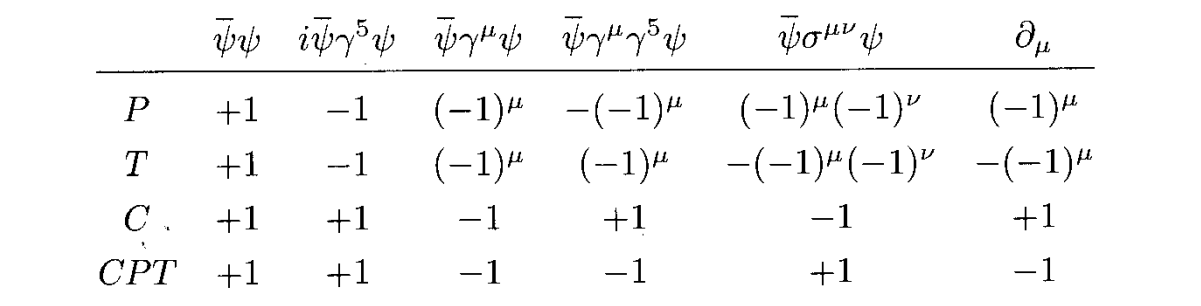
\includegraphics[height=3cm ,width=12cm]{QFT/CPT.png}
\caption{Transformation of fermion bilinears under CPT}
\end{figure}\\
\begin{newthem}[CPT theorem]
Any hermitian combination of any set of fields (scalar, vector, Dirac, Majorana) and their derivatives that is a Lorentz scalar (and so carries no indices) is even under $CPT$. Since the lagrangian must be formed out of such combinations, we
have $\mathcal{L}(x) \to \mathcal{L}(-x)$ under $CPT$, and so the action $S = \int d^4x \mathcal{L}$ is invariant.
\end{newthem}

\section{Perturbation theory for canonical quantization}
\noindent
We use Yukawa theory as an example.
\[\mathcal{L} = -\frac{1}{2}\partial_{\mu} \phi \partial^{\mu} \phi -\frac{1}{2}M_0^2 \phi^2 + i\overline{\Psi} \gamma^{\mu} \partial_{\mu} \Psi - m_0\overline{\Psi}\Psi -g_0 \overline{\Psi}\Psi\phi\]
\[H = H_0 + H_{int} \quad H_{int} = \int d^3 x \: g_0 \overline{\Psi}\Psi\phi \]
Similar to $\phi^4$ theory, the perturbation expansion of correlation functions is
\[\langle \Omega | T \{\Psi(x) \overline{\Psi}(y) \phi(z) \} | \Omega \rangle = \lim_{T \to \infty(1-i\epsilon)} \frac{\langle 0 | T \left\{ \Psi_I(x) \overline{\Psi}_I(y) \phi_I(z) \mathrm{exp} \left[ -i \int_{-T}^{T} dt H_I \right]\right\} | 0 \rangle}{\langle 0 | T \left\{ \mathrm{exp} \left[ -i \int_{-T}^{T} dt H_I \right]\right\} | 0 \rangle}\]
Before we state the Wick's theorem, we must note the following conventions:
\begin{enumerate}
\item  The time-ordered product picks up one minus sign for each
interchange of operators that is necessary to put the fields in time order.
\item The normal-ordered product picks up one minus sign for each
interchange of operators that is necessary to put the fields in normal order.
\item Define contractions under the normal-ordering symbol to include minus signs for operator interchanges.
\end{enumerate}
With these conventions, Wick's theorem takes the same form as before:
\[T \left\{ \Psi_I(x_1) \overline{\Psi}_I(x_2)  \Psi_I(x_3) \cdots \right\} = N \left\{\Psi_I(x_1) \overline{\Psi}_I(x_2)  \Psi_I(x_3) \cdots + \mbox{ all possible contractions }\right\} \]
\begin{example}
\begin{eqnarray}
\langle 0 | T \left\{ \Psi_{Ia}(x_1) \overline{\Psi}_{Ib}(x_2) \Psi_{Ic}(x_3) \overline{\Psi}_{Id}(x_4)\right\}| 0 \rangle &=& S_F(x_1-x_2)_{ab}S_F(x_3-x_4)_{cd} \nonumber \\
&-& S_F(x_1-x_4)_{ad}S_F(x_3-x_2)_{cb} \nonumber
\end{eqnarray}
\end{example}
Then we can derive the Feynman rule for Yukawa theory. 
Expand
\[\langle 0 | T \left\{ \Psi_{Ia}(x) \overline{\Psi}_{Ib}(y) \phi_I(z) \mathrm{exp} \left[ -i \int_{-T}^{T} dt H_I \right]\right\} | 0 \rangle\] 
to the first order of $g_0$
\begin{eqnarray}
& &\langle 0 | T \left\{ \Psi_{Ia}(x) \overline{\Psi}_{Ib}(y) \phi_I(z) (-i g_0) \int dw^4 \overline{\Psi}_I(w) \Psi_I(w) \phi_I(w) \right\} | 0 \rangle \nonumber \\
&=& -(-ig_0) S_F(x-y)_{ab} \int d^4 w D_F(z-w) \mathrm{Tr}[S_F(w-w)] \nonumber \\
&+&  (-ig_0) \int d^4 w  [S_F(x-w) S_F(w-y)]_{ab} D_F(w-z) \nonumber
\end{eqnarray}
It can be represented by the so called Feynman diagram.
\begin{figure}[!h]
\centering
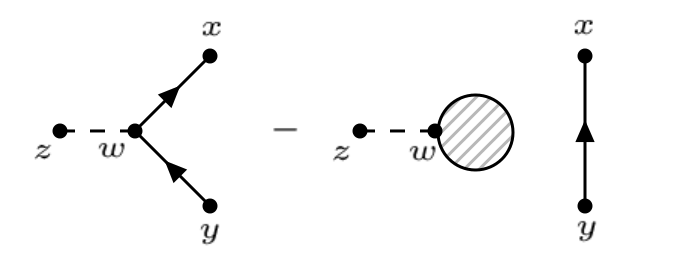
\includegraphics[height=2.6cm ,width=6.8cm]{QFT/FFD1.png}
\caption{Feynman diagram representation of perturbation expansion}
\end{figure}\\
The Feynman rules for Yukama theory are:
\begin{enumerate}
\item For each Fermion propagator from $y$ to $x$, $P = S_F(x-y)$
\item For each scalar propagator, $P = D_F(x-y)$
\item For each vertex, $V = (-ig_0)\int d^4w$
\item For each external point, $E=1$
\item Divided by the symmetry factor
\end{enumerate}

\section{Path integral quantization}
\subsection{Grassmann numbers}
\subsubsection{Formal definition}
Grassmann numbers are individual elements or points of the exterior algebra generated by a set of $n$ Grassmann variables or Grassmann directions or supercharges $\{\theta _{i}\}$ with $n$ possibly being infinite.

The Grassman variables are the basis vectors of a vector space (of dimension n) They form an algebra over a field, with the field usually being taken to be the complex numbers, although one could contemplate other fields, such as the reals. The algebra is a unital algebra, and the generators are anti-commuting:
\[\theta _{i}\theta _{j}=-\theta _{j}\theta _{i}\]
Since the $\theta _{i}$ form a vector space over the complex numbers, it is trivial that they commute with the complex numbers; this is by definition. That is, for complex x, one has
\[\theta _{i}x=x\theta _{i}\]
The squares of the generators vanish:
\[\theta_i \theta_i = -\theta_i \theta_i\]
In other words, a Grassmann variable is a non-zero square-root of zero.

Let V denote this n-dimensional vector space of Grassman variables. Note that it is independent of the choice of basis. The corresponding exterior algebra is defined as
\[\Lambda =\mathbb {C} \oplus V\oplus \left(V\wedge V\right)\oplus \left(V\wedge V\wedge V\right)\oplus \cdots\]
where $\wedge$ is the exterior product and $\oplus$ is the direct sum. The individual elements of this algebra are then called Grassman numbers. It is standard to completely omit the wedge symbol $\wedge$ when writing a Grassman number; it is used here only to clearly illustrate how the exterior algebra is built up out of the Grassman variables. Thus, a completely general Grassman number can be written as
\[z=\sum _{k=0}^{\infty }\sum _{i_{1},i_{2},\cdots ,i_{k}}c_{i_{1}i_{2}\cdots i_{k}}\theta _{i_{1}}\theta _{i_{2}}\cdots \theta _{i_{k}}\]
where the c's are complex numbers, or, equivalently, $c_{i_{1}i_{2}\cdots i_{k}}$ is a complex-valued, completely antisymmetric tensor of rank $k$. Again, the $\theta _{i}$ can be clearly seen here to be playing the role of a basis vector of a vector space.

Observe that the Grassmann algebra generated by $n$ linearly independent Grassmann variables has dimension $2n$; this follows from the binomial theorem applied to the above sum, and the fact that the $n+1$-fold product of variables must vanish, by the anti-commutation relations, above. In other words, for $n$ variables, the sum terminates
\[\Lambda =\mathbb {C} \oplus \Lambda ^{1}V\oplus \Lambda ^{2}V\oplus \cdots \oplus \Lambda ^{n}V\]
where $\Lambda ^{k}V$ is the k-fold alternating product. The dimension of  $\Lambda ^{k}V$ is given by $n$ choose $k$, the binomial coefficient. The special case of $n=1$ is called a dual number, and was introduced by William Clifford in 1873.

\subsubsection{Integral over Grassmann number}
\noindent
Single Variable:
\[\int d\theta (A + B\theta) \equiv B\]
Multi-variable:
\[\int d\theta d\eta \; \eta \theta \equiv 1\]
Complex Grassmann number:
\[(\theta \eta)^* \equiv \eta^* \theta^* = -\theta^* \eta^*\]
\[\int d\theta^* d\theta \; \theta \theta^* \equiv 1\]
Gaussian integral over a complex Grassmann number:
\[\int d\theta^* d\theta e^{-\theta^* b \theta} = b\]
\[\int d\theta^* d\theta \; \theta \theta^* e^{-\theta^* b \theta}  = 1\]
Unitary transformation:\\
If $\theta'_i = U_{ij}\theta_j$ and $U$ is unitary matrix, then we can derive
\[\prod_i \theta'_i = (\det U) (\prod_i \theta_i)\]
In a general integral
\[(\prod_i \int d\theta^*_i d\theta) f(\theta)\]
the only term of $f(\theta)$ that survives has exactly one factor of each $\theta_i$ and $\theta^*_i$; it is proportional to $(\prod_i \theta_i)(\prod_i \theta^*_i)$. If we replace $\theta$ by $U\theta$, this term acquires a factor of $\det U \det U^* = 1$, so the integral is unchanged under the unitary transformation.\\ \\
Gaussian integral over multiple complex Grassmann numbers:
\[(\prod_i \int d\theta^*_i d\theta) e^{-\theta^* B_{ij}\theta_j} = \det B\]
\[(\prod_i \int d\theta^*_i d\theta) \theta_k \theta^*_l e^{-\theta^* B_{ij}\theta_j} =B^{-1}_{kl} \det B\]

\subsection{Path integral formulation for free Dirac field}
A Grassmann field is a function of space-time whose values are Grassmann numbers. The classical Dirac field being used to evaluate path integral is a Grassmann field. The correlation function is given by
\[\langle \Omega | T \Psi_H(x_1) \overline{\Psi}_H(x_2)| \Omega \rangle = \lim_{T \to \infty(1-i\epsilon)} \frac{\int \mathcal{D}\overline{\Psi} \mathcal{D}\Psi \; \mathrm{exp} \left[ i\int_{-T}^T d^4x \overline{\Psi}(i\slashed{\partial}-m)\Psi \right] \Psi(x_1) \overline{\Psi}(x_2)}{\int \mathcal{D}\overline{\Psi} \mathcal{D}\Psi \; \mathrm{exp} \left[ i\int_{-T}^T d^4x \overline{\Psi}(i\slashed{\partial}-m)\Psi \right]}\]
The generating function is 
\[Z[\overline{\eta},\eta] = \int \mathcal{D}\overline{\Psi} \mathcal{D}\Psi \; \mathrm{exp} \left[ i\int d^4x \overline{\Psi}(i\slashed{\partial}-m)\Psi + \overline{\eta}\Psi + \overline{\Psi}\eta \right]\]
Here, $\eta(x)$ is a Grassmann-valued source field. 
Define
\[\Psi'(x) \equiv \Psi(x) - i \int d^4y S_F(x-y)\eta(y)\]
Then we can derive that
\[\overline{\Psi}'(x) \equiv \overline{\Psi}(x) - i \int d^4y \overline{\eta}(y)S_F(y-x)\]
Recall that
\[(i\slashed{\partial}_x-m)S_F(x-y) = i\delta(x-y)\]
and
\[S_F(y-x)(i \slashed{\partial}_x+m) = -i\delta(x-y)\]
we can derive that
\[\int d^4x \overline{\Psi}(i\slashed{\partial}-m)\Psi + \overline{\eta}\Psi + \overline{\Psi}\eta = \int d^4x \overline{\Psi}'(i\slashed{\partial}-m)\Psi' + i \int d^4x d^4y \overline{\eta}(x)S_F(x-y)\eta(y) \]
After integration, we have
\[Z[\overline{\eta},\eta] = Z_0 \mathrm{exp} \left[ -\int d^4x d^4y \; \overline{\eta}(x)S_F(x-y)\eta(y) \right]\]
If we adopt the convention that
\[\frac{d}{d\eta} \theta \eta = - \frac{d}{d\eta} \eta \theta = - \theta\]
the two point correlation functions are
\[\langle 0 | T \Psi_H(x_1) \overline{\Psi}_H(x_2)| 0 \rangle = Z_0^{-1} \left(-i \frac{\delta}{\delta \overline{\eta}(x_1)} \right) \left(i \frac{\delta}{\delta \eta(x_2)} \right) Z[\overline{\eta},\eta]|_{\overline{\eta},\eta=0} = S_F(x_1-x_2) \]

\subsection{Perturbation theory for path integral quantization}
\noindent
We use Yukawa theory as an example.
\begin{eqnarray}
\mathcal{L} &=& -\frac{1}{2}\partial_{\mu} \phi \partial^{\mu} \phi -\frac{1}{2}M_0^2 \phi^2 + i\overline{\Psi} \gamma^{\mu} \partial_{\mu} \Psi - m_0\overline{\Psi}\Psi -g_0 \overline{\Psi}\Psi\phi \nonumber \\
\mathcal{L} &=& \mathcal{L}_0 + \mathcal{L}_1 \quad \mathcal{L}_1 =- g_0\overline{\Psi}\Psi\phi \nonumber \\
Z[J] &=& \int \mathcal{D}\phi \mathcal{D}\overline{\Psi} \mathcal{D}\Psi e^{i\int d^4x [\mathcal{L}_0 + \mathcal{L}_1 + J\phi + \overline{\eta}\Psi \overline{\Psi}\eta]} \nonumber \\
&=& e^{i\int d^4x \mathcal{L}_1(\frac{1}{i} \frac{\delta}{\delta J(x)},\frac{1}{i}\frac{\delta}{\delta \overline{\eta}(x)},-\frac{1}{i}\frac{\delta}{\delta \eta(x)})} \int \mathcal{D}\phi \mathcal{D}\overline{\Psi} \mathcal{D}\Psi e^{i\int d^4y [\mathcal{L}_0 + J\phi]} \nonumber \\
&\propto & e^{i\int d^4x \mathcal{L}_1(\frac{1}{i} \frac{\delta}{\delta J(x)},\frac{1}{i}\frac{\delta}{\delta \overline{\eta}(x)},-\frac{1}{i}\frac{\delta}{\delta \eta(x)})} \mathrm{exp} [- \int d^4y d^4z  \frac{1}{2} J(y)D_F(y-z)J(z) + \overline{\eta}(y)S_F(y-z)\eta(z)] \nonumber \\
& =& \sum_{V=0}^{\infty} \frac{1}{V!} [-ig_0 \int d^4x (\frac{1}{i} \frac{\delta}{\delta J(x)} \cdot \frac{1}{i}\frac{\delta}{\delta \overline{\eta}(x)} \cdot -\frac{1}{i}\frac{\delta}{\delta \eta(x)})]^V \nonumber \\
&\times & \sum_{P_1=0}^{\infty} \frac{1}{P_1!} [-\frac{1}{2} \int d^4y_1 d^4z_1 J(y_1)D_F(y_1-z_1)J(z_1)]^{P_1} \nonumber \\
&\times &  \sum_{P_2=0}^{\infty} \frac{1}{P_2!} [-\int d^4y_2 d^4z_2 \overline{\eta}(y_2)S_F(y_2-z_2)\eta(z_2)]^{P_2} \nonumber
\end{eqnarray}
If we focus on a term with particular values of $V$, $P_1$ and $P_2$, then the number of surviving scalar sources is $E_1 = 2P_1-V$, the number of surviving fermion sources is $E_2 = 2P_2-2V$.
We can introduce Feynman diagrams as in the $\phi^4$ theory. In these diagrams, a dashed line segment stands for a scalar propagator $D_F(x-y)$, a line with an arrow pointing from $y$ to $x$ for a fermion propagator $S_F(x-y)$, a filled circle at one end of a dashed line segment for a scalar source $i\int d^4x J(x)$, a filled circle at the start of a line with an arrow for a fermion source $i\int d^4x \eta(x)$, a filled circle at the end of a line with an arrow for a anti-fermion source $i\int d^4x \overline{\eta}(x)$, a vertex joining three line segments for $-ig_0\int d^4x$.

\section{LSZ reduction formula}
\noindent
Similarly to the scalar field theory, we can derive the structure of the exact propagator of Dirac fermions in interaction theory.
\[\int d^4x \; e^{-ipx} \langle \Omega | T \Psi(x) \overline{\Psi}(0) | \Omega \rangle_C = \frac{iZ_2(\slashed{p}-m)}{p^2+m^2-i\epsilon} + \cdots \]
We eliminate the terms contributing none isolate poles for $p^2$. Here, $m$ is the exact mass of the fermions. The constant $Z_2$ is the probability for the quantum field to create or annihilate an exact one-particle eigenstate of $H$:
\[\langle \Omega | \Psi(0) | p,s \rangle = \sqrt{Z_2} u^s(p)\]
The LSZ reduction formula for fermions would take the form as \\ \\
\begin{newthem}[LSZ reduction formula]
\begin{eqnarray}
&\phantom{=}& \langle \bm{p}_1 \cdots \bm{p}_n \;
\overline{\bm{p}}_1 \cdots \overline{\bm{p}}_{\overline{n}} \;
| S | \;
\bm{k}_1 \cdots \bm{k}_m \;
\overline{\bm{k}}_1 \cdots \overline{\bm{k}}_{\overline{n}} \rangle 
\nonumber \\
&=& \quad \prod_1^n \int d^4 x_i e^{-i p_ix_i }
\prod_1^{\overline{n}} \int d^4 \overline{x}_i e^{-i \overline{p}_i\overline{x}_i }
\prod_1^m \int d^4 y_j e^{ik_jy_j}
\prod_1^{\overline{m}} d^4 \overline{y}_i e^{i\overline{k}_j\overline{y}_j}
\nonumber \\
&\times & [\overline{u}_{s_1}(\bm{p}_1)(\slashed{p}_1+m)] \cdots [\overline{u}_{s_n}(\bm{p}_n)(\slashed{p}_n+m)]
\nonumber \\
&\times & [\overline{v}_{\overline{r}_1}(\overline{\bm{k}}_1)(\overline{\slashed{k}}_1 - m)] \cdots [\overline{v}_{\overline{r}_{\overline{m}}}(\overline{\bm{k}}_{\overline{m}})(\overline{\slashed{k}}_{\overline{m}} - m)]
\nonumber \\
&\times & \langle \Omega | T \{\Psi(x_1) \cdots \Psi(x_n)
\overline{\Psi}(\overline{x}_1) \cdots \overline{\Psi}(\overline{x}_{\overline{n}}) 
\overline{\Psi}(y_1) \cdots \overline{\Psi}(y_m)
\Psi(\overline{y}_1) \cdots \Psi(\overline{y}_{\overline{m}})\} 
| \Omega \rangle 
\nonumber \\
&\times & [(\slashed{k}_1+m) u_{r_1}(\bm{k}_1)] \cdots [(\slashed{k}_m+m)u_{r_m}(\bm{k}_m)] \nonumber \\
&\times & [(\overline{\slashed{p}}_1 - m) v_{\overline{s}_1}(\overline{\bm{p}}_1)] \cdots [(\overline{\slashed{p}}_{\overline{n}} - m) v_{\overline{s}_{\overline{n}}}(\overline{\bm{p}}_{\overline{n}})] \nonumber \\
&\times & \left( \frac{i}{\sqrt{Z}_2} \right) ^{m+\overline{m}+n+\overline{n}} \nonumber
\end{eqnarray}
\end{newthem}
From this equation, we can see that the scattering amplitude would vanish unless $n+\overline{m} = \overline{n} + m$, which implies the conservation of $Q$. The term $e^{ipx}$ will impose the condition of momentum conservation, and the the term $\slashed{p}\pm m$ will remove the external legs. \\
Finally, we list the Feymann rules of Yukawa theory in momentum space as follows:
\begin{enumerate}
\item For each incoming electron, draw a solid line with an arrow pointed towards the vertex, and label it with the electron's four-momentum, $k_i$.
\item For each outgoing electron, draw a solid line with an arrow pointed away from the vertex, and label it with the electron's four-momentum, $p_i$.
\item For each incoming positron, draw a solid line with an arrow pointed away from the vertex, and label it with minus the positron's four-momentum, $-\bar{k}_i$.
\item For each outgoing positron, draw a solid line with an arrow pointed towards the vertex, and label it with minus the positron's four-momentum, $-\bar{p}_i$.
\item For each incoming scalar, draw a dashed line with an arrow pointed towards the vertex, and label it with the scalar's four-momentum, $q_i$.
\item For each outgoing scalar, draw a dashed line with an arrow pointed away from the vertex, and label it with the scalar's four-momentum, $q'_i$.
\item The only allowed vertex joins two solid lines, one with an arrow pointing towards it and one with an arrow pointing away from it, and one dashed line (whose arrow can point in either direction). Using this vertex, join up all the external lines, including extra internal lines as needed. In this way, draw all possible diagrams that are topologically inequivalent.
\item Assign each internal line its own four-momentum. Think of the four-momenta as flowing along the arrows, and conserve four-momentum at each vertex. For a tree diagram, this fixes the momenta on all the internal lines.
\item The value of a diagram consists of the following factors:
\begin{itemize}
\item for each incoming or outgoing scalar, $1$;
\item for each incoming electron, $u_{r}(\bm{k})$;
\item for each outgoing electron, $\overline{u}_{s}(\bm{p})$;
\item for each incoming positron, $\overline{v}_{\overline{r}}(\overline{\bm{k}})$;
\item for each outgoing positron, $v_{\overline{s}}(\overline{\bm{p}})$;
\item for each vertex, $-ig_0$;
\item for each internal scalar, $\frac{-i}{p^2+M^2-i\epsilon}$;
\item for each internal fermion, $\frac{i(\slashed{p}-m)}{p^2+m^2-i\epsilon}$
\end{itemize}
\item Spinor indices are contracted by starting at one end of a fermion line: specifically, the end that has the arrow pointing away from the vertex. The factor associated with the external line is either $\bar{u}$ or $\bar{v}$. Go along the complete fermion line, following the arrows backwards, and write down (in order from left to right) the factors associated with the vertices and propagators that you encounter. The last factor is either a $u$ or $v$. Repeat this procedure for the other fermion lines, if any.
\item The overall sign of a tree diagram is determined by drawing all contributing diagrams in a standard form: all fermion lines horizontal, with their arrows pointing from left to right, and with the left endpoints labeled in the same fixed order (from top to bottom); if the ordering of the labels on the right endpoints of the fermion lines in a given diagram is an even (odd) permutation of an arbitrarily chosen fixed ordering, then the sign of that diagram is positive (negative).
\item Each closed fermion loop contributes an extra minus sign.
\item Value of $i\mathcal{M}$ is given by a sum over the values of the contributing diagrams.
\item $\langle f | S | i \rangle = i\mathcal{M}\delta(\sum p_f -\sum p_i)$
\end{enumerate}

\section{Renormalization}
\noindent
The full Lagrangian of Yukawa theory is
\[\mathcal{L} = -\frac{1}{2}\partial_{\mu} \phi \partial^{\mu} \phi -\frac{1}{2}M_0^2 \phi^2 + i\overline{\Psi} \gamma^{\mu} \partial_{\mu} \Psi - m_0\overline{\Psi}\Psi - a_0\phi -\frac{1}{3!}b_0\phi^3 -\frac{1}{4!}c_0 \phi^4 -g_0 \overline{\Psi}\Psi\phi\]
Suppose the number of external lines of scalar is $N_1$, the number of external lines of fermions is $N_2$, the number of scalar propagator (after amputation) is $P_1$, the number of fermion propagator is $P_2$, the number of vertex is $V_a$,$V_b$,$V_c$ and $V_g$. So we know the number of loops is
\[L = P_1+P_2-V_a -V_b-V_c-V_g+1\]
We also know that
\[V_a + 3V_b + 4V_c + V_g = 2P_1 + N_1  \quad 2V_g = 2P_2 + N_2\]
So, the superficial divergence is 
\[D = 4L - 2P_1 - P_2 = 4 -N_1 - \frac{3}{2}N_2 - 3V_a - V_b\]
So, Yukawa theory is a renormalizable theory. Only a finite number of amplitudes superficially diverge; however, divergences occur at all orders in perturbation theory. The only divergent amplitudes (except vacuum energy) are therefore
\begin{figure}[!h]
\centering
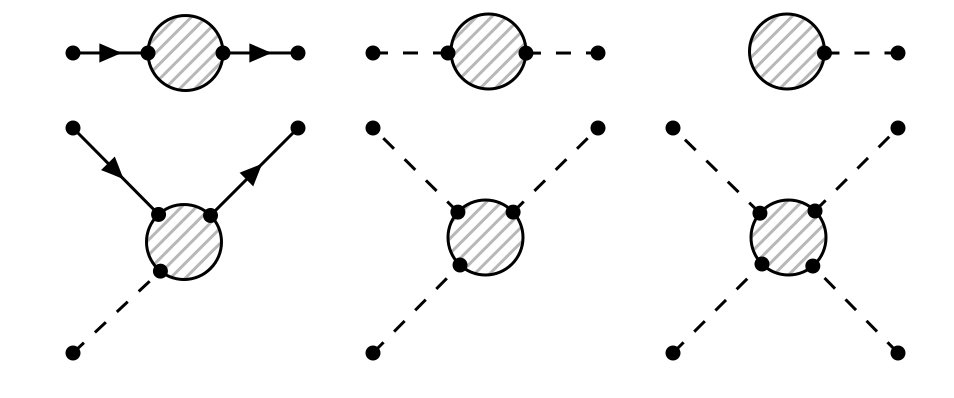
\includegraphics[height=4cm ,width=9.5cm]{QFT/DRG1.png}
\caption{Divergence of Yukawa theory}
\end{figure}\\
There are six kinds of divergent diagrams, including two propagators. So, we can use eight counter terms to absorb all the infinities order by order. The Lagrangian can be written as
\[\mathcal{L} = \mathcal{L}_1 + \mathcal{L}_{ct}\]
Here,
\[\mathcal{L}_1 = -\frac{1}{2}\partial_{\mu} \phi_r \partial^{\mu} \phi_r -\frac{1}{2}M^2 \phi_r^2 + i\overline{\Psi}_r \gamma^{\mu} \partial_{\mu} \Psi_r - m \overline{\Psi}_r \Psi_r - a\phi_r- \frac{1}{3!}b\phi_r^3 -\frac{1}{4!}c \phi_r^4 -g \overline{\Psi}_r\Psi_r\phi_r \]
\[\mathcal{L}_{ct} = -\frac{1}{2}\delta_{Z_1}\partial_{\mu} \phi_r \partial^{\mu} \phi_r -\frac{1}{2}\delta_M \phi_r^2 + i\delta_{Z_2}\overline{\Psi}_r \gamma^{\mu} \partial_{\mu} \Psi_r - \delta_m \overline{\Psi}_r \Psi_r - \delta_a\phi_r- \frac{1}{3!}\delta_b\phi_r^3 -\frac{1}{4!}\delta_c \phi_r^4 -\delta_g \overline{\Psi}_r\Psi_r\phi_r \]
\[\phi = \sqrt{Z_1}\phi_r \quad \Phi  = \sqrt{Z_2}\Phi_r \quad \delta_{Z_1} = Z_1 - 1 \quad \delta_{Z_2} = Z_2 - 1 \quad \delta_M = Z_1 M_0^2 - M^2\]
\[\delta_m = Z_2 m_0^2 - m^2 \quad \delta_a = \sqrt{Z_1}a_0 - a \quad \delta_b = \sqrt[3]{Z_1} b_0 - b \quad \delta_c= Z_1^2 c_0 - c \quad \delta_g = \sqrt{Z_1}Z_2 g_0 - g\]

The Feymann rules for most counter terms will be similar to those in $\phi^4$ theory. We only need to notice that the vertex value of the term  $i\delta_{Z_2}\overline{\Psi}_r \gamma^{\mu} \partial_{\mu} \Psi_r - \delta_m \overline{\Psi}_r \Psi_r $ is
\[-i(\delta_{Z_2} \slashed{p} + \delta m)\]

Then we can use either on-shell renormolization scheme or $\overline{MS}$ renormalization scheme to get renormalization conditions. 
We would mention the diagram representation of exact fermion propagator. If we denote the sum of all 1PI diagrams with two external fermion lines as $-i\Sigma$, then the full propagator will take the form as
\[\frac{-i}{\slashed{p}+m+\Sigma(\slashed{p})}\]
The on-shell renormolization scheme condition implies that
\[\Sigma(\slashed{p})_{\slashed{p}=-m} = 0 \quad \left(\frac{d\Sigma}{d\slashed{p}}\right)_{\slashed{p} = -m} = 0\]

We can adjust the counter terms as necessary to maintain the renormalization conditions. After this adjustment, the expression for the amplitude should be finite and independent of the regulator.

The one loop structure of Yukawa theory is somewhat complicated and will not be discussed here. The chapter 51 and 52 from \emph{Quantum Field Theory (Mark Srednicki)} will discussed the one loop structure and beta function of a modified Yukawa theory.
\chapter{Vector Field}
\section{Vector field}
Consider a vector field $A^{\mu}(x)$. Here the index $\mu$ is a vector index that takes on four possible values. Under a Lorentz transformation, we have
\[U(\Lambda)^{-1} A^{\mu}(x) U(\Lambda) = \Lambda^{\mu}_{\phantom{\mu}\nu} A^{\nu}(\Lambda^{-1}x)\]
For an infinitesimal transformation, we can write
\[\delta^{\mu}_{\phantom{\mu}\nu}+\delta \omega ^{\mu}_{\phantom{\mu}\nu} = \delta^{\mu}_{\phantom{\mu}\nu} + \frac{i}{2} \delta \omega_{\rho \sigma} (S_V^{\rho \sigma})^{\mu}_{\phantom{\mu}\nu}\]
Here
\[(S_V^{\rho \sigma})^{\mu}_{\phantom{\mu}\nu} = -i(\eta^{\rho \mu}\delta ^{\sigma}_{\phantom{\sigma}\nu} - \eta^{\sigma \mu}\delta^{\rho}_{\phantom{\rho}\nu})\]
It is obvious that $A^{\dagger \mu}$ is also a vector field. 
We know that $\eta^{\mu \nu}$ is invariant under Lorentz transformation, i.e.
\[\Lambda^{\mu}_{\phantom{\mu}\rho} \Lambda^{\nu}_{\phantom{\mu}\sigma} \eta^{\rho \sigma} = \eta^{\mu \nu} \]
We can use $\eta^{\mu \nu}$ and and its inverse $\eta_{\mu\nu}$ to raise and lower vector indices of the vector field,
\[A_{\mu} \equiv \eta_{\mu \nu} A^{\nu}\]
And we can verify the following equations
\[\Lambda^{\mu}_{\phantom{\mu}\nu} \Lambda_{\mu}^{\phantom{\mu}\rho} = \delta^{\rho}_{\nu} \]
\[A^{\mu}(x) = \eta^{\mu \nu} A_{\nu}(x)\]
\[\Lambda_{\mu}^{\phantom{\mu}\rho} \Lambda_{\nu}^{\phantom{\nu}\sigma} \eta_{\rho \sigma} = \eta_{\mu \nu}\]
\[U(\Lambda)^{-1} A_{\mu}(x) U(\Lambda) = \Lambda_{\mu}^{\phantom{\mu}\nu} A_{\nu}(\Lambda^{-1}x)\]
Define $C_i \equiv \frac{1}{2}\epsilon_{ijk}S_V^{jk}$,$D_i \equiv S_V^{i0}$. For example, we have
\[(C_3)_{\mu}^{\phantom{\mu}\nu} = \left(\begin{array}{rrrr}
0 & 0 & 0 & 0 \\
0 & 0 & -i & 0 \\
0 & i & 0 & 0 \\
0 & 0 & 0 & 0
\end{array}\right)\]
The eigenvectors of $C_3$ are
\[\left[\left(-1, \left[\left(0,\,1,\,-i,\,0\right)\right], 1\right),
\left(1, \left[\left(0,\,1,\,i,\,0\right)\right], 1\right), \left(0,
\left[\left(1,\,0,\,0,\,0\right), \left(0,\,0,\,0,\,1\right)\right],
2\right)\right]\]
We further define $N_i \equiv \frac{1}{2}(C_i-iD_i)$ and $N^{\dagger}_i \equiv \frac{1}{2}(C_i + i D_i)$. For example, we have
\[(N_1)_{\mu}^{\phantom{\mu}\nu} = \left(\begin{array}{rrrr}
0 & -\frac{1}{2} & 0 & 0 \\
-\frac{1}{2} & 0 & 0 & 0 \\
0 & 0 & 0 & -\frac{1}{2} i \\
0 & 0 & \frac{1}{2} i & 0
\end{array}\right)\]
The eigenvectors of $N_1$ are
\[\left[\left(-\frac{1}{2}, \left[\left(1,\,1,\,0,\,0\right),
\left(0,\,0,\,1,\,-i\right)\right], 2\right), \left(\frac{1}{2},
\left[\left(1,\,-1,\,0,\,0\right), \left(0,\,0,\,1,\,i\right)\right],
2\right)\right]\]
And we can conclude that vector is in the $(2,2)$ representation of the Lie algebra of the Lorentz group.

\section{Electromagnetic field and gauge invariance}
\noindent
The Lagrangian of EM field is
\[\mathcal{L} = -\frac{1}{4}F_{\mu\nu}F^{\mu\nu}\]
Here,
\[F_{\mu\nu} = \partial_{\mu} A_{\nu} - \partial_{\nu} A_{\mu} \quad \mbox{and} \quad A^{\mu} = (\phi,\bm{A})\]
So,
\[F_{0i} = \dot{A}^i + \nabla_i \phi \equiv -E^i \quad \mbox{and} \quad F_{ij} = \nabla_i A^j - \nabla_j A^i \equiv \epsilon_{ijk}B^k\]
We can derive the equation of motion of the EM field by variation method,
\[\partial_{\mu}F^{\mu \nu} = 0\]
It can be rewritten in terms of $\bm{E}$ and $\bm{B}$, i.e. Maxwell equations:
\begin{eqnarray}
&\phantom{=}&\bm{\nabla} \cdot \bm{E} = 0 \quad \frac{\partial \bm{E}}{\partial t} = \bm{\nabla} \times \bm{B} \nonumber \\
&\phantom{=}& \bm{\nabla} \cdot \bm{B} = 0  \quad \frac{\partial \bm{B}}{\partial t} = - \bm{\nabla} \times \bm{E}\nonumber
\end{eqnarray}

The massless vector field $A_{\mu}$ has 4 components, which would naively seem to tell us that the gauge field has 4 degrees of freedom.But there are two related comments which will ensure that quantizing the gauge field $A_{\mu}$ gives rise to 2 degrees of freedom, rather than 4.
\begin{itemize}
\item The field $A_0$ has no kinetic term $\dot{A_0}$ in the Lagrangian: it is not dynamical. This means that if we are given some initial data $A_i$ and $\dot{A_i}$ at a time $t_0$, then the field $A_0$ is fully determined by the equation of motion $\bm{\nabla} \cdot \bm{E} = 0$,which, expanding out,
reads
\[\nabla^2 A_0 = \bm{\nabla} \cdot \frac{\partial \bm{A}}{\partial t}\]
So $A_0$ is not independent: we don't get to specify $A_0$ on the initial time slice.
\item If we transform the EM field as
\[A_{\mu} \to A_{\mu} + \partial_{\mu}\lambda(x) \]
we can derive that
\[F_{\mu\nu} \to F_{\mu \nu} \quad \mathcal{L} \to \mathcal{L}\]
The seemed infinite number of symmetries, one for each function $\lambda(x)$, is to be viewed as a redundancy in our description. That is, two states related by a gauge symmetry are to be identified: they are the same physical state. One way to see that this interpretation is necessary is to notice that Maxwell’s equations are not sufficient to specify the evolution of $A_{\mu}$.The equations read,
\[(\eta_{\mu\nu} \partial^2 - \partial_{\mu} \partial_{\nu}) A^{\nu} = 0\]
But the operator $(\eta_{\mu\nu} \partial^2 - \partial_{\mu} \partial_{\nu})$ is not invertible: it annihilates any function of
the form $\partial_{\mu} \lambda$. This means that given any initial data, we have no way to uniquely determine $A_{\mu}$ at a later time since we can't distinguish between $A_{\mu}$ and $A_{\mu} + \partial_{\mu} \lambda$. This would be problematic if we thought that $A_{\mu}$ is a physical object. However, if we're happy to identify $A_{\mu}$ and $A_{\mu} + \partial_{\mu} \lambda$ as corresponding to the same physical state, then our problems disappear. 
\end{itemize}

The picture that emerges for the theory of electromagnetism is of an enlarged phase space, foliated by gauge orbits. All states that lie along a given gauge orbit can be reached by a gauge transformation and are identified. To make progress, we pick a representative from each gauge orbit. It doesn't matter which representative we pick after all, they're all physically equivalent. But we should make sure that we pick a "good" gauge, in which we cut the orbits. Here we'll look at two different gauges:
\begin{itemize}
\item Coulomb Gauge: $\bm{\nabla} \cdot \bm{A} = 0$\\
We can make use of the residual gauge transformations in Lorentz gauge to pick $\bm{\nabla} \cdot \dot{\bm{A}} = 0$. We
have as a consequence $A_0 = 0$. Coulomb gauge is sometimes called radiation gauge.
\item Lorentz Gauge: $\partial^{\mu} A_{\mu} = 0$\\
In fact this condition doesn't pick a unique representative from the gauge orbit. We're always free to make further gauge transformations with $\partial^{\mu}\partial_{\mu} \lambda = 0$, which also has non-trivial solutions. As the name suggests, the Lorentz gauge has the advantage that it is Lorentz invariant.
\end{itemize}

\section{Canonical quantization of EM field}
\subsection{Canonical quantization in Coulomb gauge}

\subsubsection{Canonical momentum and Hamiltonian}
\[\pi^0 = \frac{\partial \mathcal{L}}{\partial \dot{A_0}} = 0 \quad  \pi^{i} = \frac{\partial \mathcal{L}}{\partial(\partial_0 A_i)} = \dot{A}^i + \nabla_i \phi = -E^i\]
\[\mathcal{H} = \frac{1}{2}(\bm{\pi}^2 + \bm{B}^2) + (\bm{\pi} \cdot \bm{\nabla}) A_0\]
Integration by parts can give
\[H = \int d^3x \frac{1}{2}(\bm{\pi}^2 + \bm{B}^2)\]

\subsubsection{Momentum and angular momentum}
\[P^0 = H \quad \vec{P} = \int - \bm{\pi} \vec{\nabla} \bm{A} d^3x\]
\[\vec{J} = - \int \bm{\pi} (\vec{x}\times \vec{\nabla} + i \vec{C})\bm{A} \; d^3x \quad \vec{S} = -i \int \bm{\pi} \vec{C} \bm{A} \; d^3x\]

\subsubsection{Canonical quantization}
\noindent
In Coulomb gauge, we have
\[A_0 = \pi^0 = 0 \quad \pi^i = \dot{A}^i \]
Three pairs of $A_i$ and $\pi^i$ are not independent from each other. They must satisfy the constraint equations
\[\nabla \cdot \bm{A} = 0 \quad \nabla \cdot \bm{\pi} = 0\]
A reasonable quantization condition can be written as
\[[A_i(\bm{x},t),A_j(\bm{x}',t)] = 0 \quad [\pi^i(\bm{x},t),\pi^j(\bm{x}',t)] = 0\]
\[[A_i(\bm{x},t),\pi^j(\bm{x}',t)] = i \left( \delta^{j}_i - \frac{\partial_i \partial^j}{\nabla^2} \right) \delta(\bm{x}-\bm{x}') \equiv i \int \frac{d^3k}{(2\pi)^3} \; (\delta^j_i - \frac{k_ik^j}{\bm{k}^2})e^{i\bm{k}\cdot(\bm{x}-\bm{x}')}\]
In this case, we can verify that
\[\dot{A}_i = -i[A_i(\bm{x},t),H] = \pi_i (\bm{x},t)\]
\[\dot{\pi}^i = -i[\pi^i(\bm{x},t),H] = \nabla^2 A^i(\bm{x},t)\]
It is constant with the field equation we derive from Euler-Lagrange equation.

\subsubsection{Fourier expansion}
\[\bm{A}(x) = \sum_{r = \pm} \int \widetilde{dp} [a_{r}(\bm{p}) \bm{\epsilon}_r(\bm{p})e^{ipx} + a^{\dagger}_{r}(\bm{p}) \bm{\epsilon}^*_r(\bm{p})e^{-ipx}]\]
And we can derive from constraint condition that
\[\bm{\epsilon} \cdot \bm{p} = 0\]
We will choose $\bm{\epsilon}$ to satisfy that
\[\bm{\epsilon}_r \cdot \bm{\epsilon}^*_s = \delta_{rs}\]
So, the completeness relation for the polarization vectors is
\[\sum_{r=\pm} \epsilon_r^i(\bm{p}) \epsilon_r^{*j}(\bm{p}) = \delta^{ij} - \frac{p^ip^j}{|\bm{p}|^2}\]
\begin{example}
If $\bm{p} = (0,0,p)$, we usually choose 
\[\bm{\epsilon}_{+} = \frac{1}{\sqrt{2}}(1,i,0) \quad \bm{\epsilon}_{-} = \frac{1}{\sqrt{2}}(1,-i,0) \]
$\bm{\epsilon}_{+}$ corresponds to left-handed rotation and it is the eigenvectors of the space-part of $C_3$ with eigenvalue $+1$. $\bm{\epsilon}_{-}$ corresponds to right-handed rotation and it is eigenvector of the space-part of $C_3$ with eigenvalue $- 1$.
\end{example}
\noindent
We can further derive from above discussion that
\[\bm{\pi}(x) = -i \sum_{r = \pm} \int \widetilde{dp} \omega [a_{r}(\bm{p}) \bm{\epsilon}_r(\bm{p})e^{ipx} - a^{\dagger}_{r}(\bm{p}) \bm{\epsilon}^*_r(\bm{p})e^{-ipx}]\]
\[a_r(\bm{p}) = \bm{\epsilon}^*_r \int d^3x e^{-ikx}(i\bm{\pi}+\omega\bm{A})\]
\[a^{\dagger}_r(\bm{p}) = \bm{\epsilon}_r \int d^3x e^{ikx}(-i\bm{\pi}+\omega\bm{A})\]
\[[a_r(\bm{p}),a_{r'}(\bm{p'})] = 0 \quad [a^{\dagger}_r(\bm{p}),a^{\dagger}_{r'}(\bm{p'})] = 0 \quad [a_r(\bm{p}),a^{\dagger}_{r'}(\bm{p'})] = (2\pi)^3 2\omega \delta_{rr'} \delta(\bm{p} - \bm{p}')\]

\subsubsection{Operator represented by $a$ and $a^{\dagger}$}
\noindent
Define that
\[N(\bm{p},r) \equiv a^{\dagger}_{r}(\bm{p}) a_r(\bm{p})\]
So, we can derive
\[H = \sum_{r = \pm} \int \widetilde{dp} \; \omega N(\bm{p},r) + 2\mathcal{E}_0V\]
\[\vec{P} = \sum_{r = \pm} \int \widetilde{dp} \; \vec{p} N(\bm{p},r) \]
\[\vec{S} = \sum_{r,s = \pm} \int \widetilde{dp} \; \frac{1}{2}(\bm{\epsilon}^*_{s} \vec{C}\bm{\epsilon}_{r} - \bm{\epsilon}_{r} \vec{C}\bm{\epsilon}^*_{s}) a^{\dagger}_{s}(\bm{p}) a_r(\bm{p})\]
From above equation, we can say that $a^{\dagger}_r(\bm{p})$ create an photon with energy $\omega$, momentum $\bm{p}$ and spin angular momentum along the direction of momentum $r$.

\subsubsection{Propagator}
\[G_{ij} \equiv \langle 0 |T A_i(x) A_j(y) | 0 \rangle = \int \frac{d^4p}{(2\pi)^4} \frac{-i}{p^2-i\epsilon} \left(\delta_{ij} - \frac{p_ip_j}{|\bm{p}|^2}\right) e^{ip(x-y)}\]

\subsection{Canonical quantization in Lorentz gauge}
\subsubsection{Undefined metric formalism}
\noindent
Modify the Maxwell Lagrangian introducing a new term
\[\mathcal{L} = -\frac{1}{4} F_{\mu\nu}F^{\mu\nu} - \frac{1}{2\xi} (\partial_{\mu} A^{\mu})^2\]
The equations of motion are now
\[\partial^2 A_{\mu} - (1-\frac{1}{\xi})\partial^{\mu}(\partial \cdot A) = 0\]
Canonical momentums are
\[\pi^0 = \frac{1}{\xi} \partial \cdot A = \frac{1}{\xi}(-\dot{A}_0 + \partial_i A^i) \quad \pi^i = \dot{A}^i + \nabla^i A^0 = -E^i\]
Hamiltonian is
\[\mathcal{H} = \frac{1}{2}(\bm{\pi}^2 + \bm{B}^2 - \xi \pi^0 \pi^0) + (\bm{\pi} \cdot \bm{\nabla}) A_0 + \pi^0 (\bm{\nabla} \cdot \bm{A})\]
\[H =  \int \left[ \frac{1}{2}(\bm{\pi}^2 + \bm{B}^2 - \xi \pi^0 \pi^0) -A_0(\bm{\nabla} \cdot \bm{\pi}) + \pi^0 (\bm{\nabla} \cdot \bm{A}) \right] d^3x \]
We remark that the above Lagrangian and the equations of motion, reduce to Maxwell theory in the gauge $\partial \cdot A = 0$. This why we say that our choice corresponds to a class of Lorenz gauges with parameter $\xi$. With this abuse of language (in fact we are not setting $\partial \cdot A = 0$, otherwise the problems would come back) the value of $\xi=1$ is known as the Feynman gauge and $\xi=0$ as the Landau gauge. From now on we will take the case of the so-called Feynman gauge, where $\xi=1$. Then the equation of motion coincide with the Maxwell theory in the Lorenz gauge. In Feymann gauge,the canonical quantization conditions can be written as
\[[A_{\mu}(\bm{x},t),A_{\nu}(\bm{x}',t)] = 0 \quad [\pi^{\mu}(\bm{x},t),\pi^{\nu}(\bm{x}',t)] = 0 \quad [A_{\mu}(\bm{x},t),\pi^{\nu}(\bm{x}',t)] = i\delta^{\nu}_{\mu} \delta(\bm{x}-\bm{x}')\]
we can also derive that
\[[\dot{A}_{\mu}(\bm{x},t),\dot{A}_{\nu}(\bm{x}',t)] = 0 \quad [A_{\mu}(\bm{x},t),\dot{A}_{\nu}(\bm{x}',t)] = i\eta_{\mu\nu} \delta(\bm{x}-\bm{x}')\]

\subsubsection{Fourier expansion}
\[A(x) = \sum_{\lambda=0}^{3} \int \widetilde{dp} [a_{\lambda}(\bm{p}) \epsilon_{\lambda}(\bm{p})e^{ipx} + a^{\dagger}_{\lambda}(\bm{p}) \epsilon^*_{\lambda}(\bm{p})e^{-ipx}]\]
where $\epsilon_{\lambda \mu}$ are a set of four independent 4-vectors.  We will now make a choice for these 4-vectors. We choose $\epsilon_{1\mu}$ and $\epsilon_{2\mu}$ orthogonal to $k^{\mu}$ and $n^{\mu}$, such that
\[\epsilon_{\lambda \mu} \epsilon^{*\mu}_{\lambda} = \delta_{\lambda \lambda'} \quad \lambda,\lambda' = 1,2\]
After, we choose $\epsilon_{3\mu}$ in the plane $(k^{\mu},n^{\mu})$ and perpendicular to $n^{\mu}$ such that
\[\epsilon_{3\mu} n^{\mu} = 0 \quad \epsilon_{3\mu} \epsilon^{*\mu}_{3} = 1\]
Finally we choose $\epsilon_{0\mu} = n_{\mu}$. The vectors $\epsilon_{1\mu}$ and $\epsilon_{2\mu}$ are called transverse polarizations, while $\epsilon_{3\mu}$ and $\epsilon_{0\mu}$ longitudinal and scalar polarizations, respectively.\\
In general we can show that
\[\epsilon_{\lambda} \cdot \epsilon^*_{\lambda'} = \eta_{\lambda \lambda'} \quad \eta^{\lambda \lambda'} \epsilon_{\lambda \mu} \epsilon^*_{\lambda' \nu} = \eta_{\mu \nu} \]
We can further derive from above discussion that
\[\dot{A}(x) = -i \sum_{\lambda=0}^{3} \int \widetilde{dp} \omega [a_{\lambda}(\bm{p}) \epsilon_{\lambda}(\bm{p})e^{ipx} - a^{\dagger}_{\lambda}(\bm{p}) \epsilon^*_{\lambda}(\bm{p})e^{-ipx}]\]
\[ a_{\lambda}(\bm{p}) =  \eta_{\lambda \lambda'} \epsilon^*_{\lambda'} \cdot \int d^3x e^{-ipx}(i\dot{A}+\omega A)\]
\[ a^{\dagger}_{\lambda}(\bm{p}) =  \eta_{\lambda \lambda'} \epsilon_{\lambda'} \cdot \int d^3x e^{ipx}(-i\dot{A}+\omega A)\]
\[[a_{\lambda}(\bm{p}),a_{\lambda'}(\bm{p'})] = 0 \quad [a^{\dagger}_{\lambda}(\bm{p}),a^{\dagger}_{\lambda'}(\bm{p'})] = 0 \quad [a_{\lambda}(\bm{p}),a^{\dagger}_{\lambda'}(\bm{p'})] = (2\pi)^3 2\omega \eta_{\lambda \lambda'} \delta(\bm{p} - \bm{p}')\]

\subsubsection{Indefinite metric problem}
We Introduce the vacuum state defined by
\[a_{\lambda}(\bm{p}) | 0 \rangle = 0\]
To see the problem with the sign we construct the one-particle state with scalar polarization, that is
\[|1\rangle = \int \widetilde{dp} a^{\dagger}_{0}(\bm{p})|0\rangle
\]
and calculate its norm
\[\langle 1 | 1 \rangle = -\langle 0 | 0 \rangle \int \widetilde{dp} |f(p)|^2\]
The state $| 1 \rangle$ has a negative norm.

To solve this problem we note that we are not working anymore with the classical Maxwell theory because we modified the Lagrangian. What we would like to do is to impose the condition $\partial \cdot A = 0$, but that is impossible as an equation for operators. We can, however, require that condition on a weaker form, as a condition only to be verified by the physical states.

More specifically, we require that the part of $\partial \cdot A$ that contains the annihilation operator (positive frequencies) annihilates the physical states,
\[\partial^{\mu} A^{+}_{\mu} | \psi \rangle = 0\]
The states $| \psi \rangle$ can be written in the form
\[| \psi \rangle = | \psi_T \rangle | \phi \rangle\]
where $| \psi_T \rangle$  is obtained from the vacuum with creation operators with transverse polarization and $| \phi \rangle$ with scalar and longitudinal polarization.

$\partial^{\mu} A^{+}_{\mu}$ contains only scalar and longitudinal polarizations
\[\partial^{\mu} A^{+}_{\mu} = i\sum_{\lambda=0,3} \int \widetilde{dp} a_{\lambda}(\bm{p}) (p \cdot \epsilon_{\lambda}(\bm{p}) ) e^{ipx} \]
Therefore the previous condition becomes
\[i\sum_{\lambda=0,3} (p \cdot \epsilon_{\lambda}(\bm{p})) a_{\lambda}(\bm{p})  | \phi \rangle = 0\]
The condition is equivalent to,
\[(a_{0}(\bm{p}) - a_{3}(\bm{p})) | \phi \rangle = 0\]
We can construct $| \phi \rangle$ as a linear combination of states $| \phi \rangle$ with $n$ scalar or longitudinal photons:
\[| \phi \rangle = C_0 | \phi_0 \rangle + C_1 | \phi \rangle + \cdots \quad \mbox{Here,} | \phi_0 \rangle \equiv | 0 \rangle\]
The states $|\phi_n\rangle$ are eigenstates of the operator number for scalar or longitudinal photons
\[N' | \phi_n \rangle = n | \phi_n \rangle\]
where,
\[N' = \int \widetilde{dp} [a^{\dagger}_{3}(\bm{p})a_{3}(\bm{p})-a^{\dagger}_{0}(\bm{p})a_{0}(\bm{p})] \]
Then
\[n \langle \phi_n | \phi_n \rangle = \langle \phi_n |N'| \phi_n \rangle = 0\]
This means that
\[\langle \phi_n | \phi_n \rangle = \delta_{n0}\]
that is, for $n \neq 0$, the state $| \phi_n \rangle$ has zero norm. We have then for the general state $| \phi \rangle$,
\[\langle \phi | \phi \rangle = |C_0|^2 \geq 0\]
and the coefficients $C_i(i=1,2,\cdots)$ are arbitrary.

\subsubsection{Operator represented by $a$ and $a^{\dagger}$}
\noindent
Define that
\[N'(\bm{p}) \equiv a^{\dagger}_{3}(\bm{p})a_{3}(\bm{p})-a^{\dagger}_{0}(\bm{p})a_{0}(\bm{p})\]
\[N(\bm{p},1) \equiv a^{\dagger}_{1}(\bm{p}) a_{1}(\bm{p}) \quad N(\bm{p},2) \equiv a^{\dagger}_{2}(\bm{p}) a_{2}(\bm{p}) \quad N_T(\bm{p}) \equiv N(\bm{p},1) + N(\bm{p},2)\]
We have that
\[\langle \psi | N'(\bm{p}) | \psi\rangle = 0 \quad \langle \psi | N_T(\bm{p}) | \psi\rangle = \langle \psi_T | N_T(\bm{p}) | \psi_T\rangle\]
We can derive
\[ H = \int \widetilde{dp} \; \omega [N'(\bm{p}) + N_T(\bm{p})] + 2\mathcal{E}_0V\]
\[ \vec{P} = \int \widetilde{dp} \; \vec{p} [N'(\bm{p}) + N_T(\bm{p})]\]

So, the arbitrariness of $C_i(i=1,2,\cdots)$ does not affect the physical observables. Only the physical transverse polarizations
contribute to the result. Two states that differ only in their timelike and longitudinal photon content, $|\phi_n\rangle$ with $n \geq 1$ are said to be physically equivalent. We can think of the gauge symmetry of the classical theory as descending to the Hilbert space of the quantum theory.

It is important to note that although for the average values of the physical observables only the transverse polarizations contribute, the scalar and longitudinal polarizations are necessary for the consistency of the theory. In particular they show up when we consider complete sums over the intermediate states.

\subsubsection{Propagator}
\[G_{\mu\nu} \equiv \langle 0 |T A_{\mu}(x) A_{\nu}(y) | 0 \rangle = \int \frac{d^4p}{(2\pi)^4} \frac{-i\eta_{\mu\nu}}{p^2-i\epsilon}  e^{ip(x-y)}\]
It is easy to verify that $G_{\mu\nu}(x-y)$ is the Green's function of the equation of motion, that for $\xi=1$ is the wave equation, that is
\[\partial^2 G_{\mu\nu} = i\eta_{\mu\nu}\delta(x-y)\]
For the general case, $\xi \neq 0$, the equal times commutation relations are more complicated. And the propagator will be
\[G_{\mu\nu}  = \int \frac{d^4p}{(2\pi)^4} \left[\frac{-i\eta_{\mu\nu}}{p^2-i\epsilon} + i(1-\xi)\frac{k_{\mu}k_{\nu}}{(k^2-i\epsilon)^2}\right] e^{ip(x-y)}\]

\end{document}